% !TeX root = main.tex

\documentclass[openright,twoside,headsepline,bibliography=totoc]{scrbook}
% The document is a book with a few options:
%   openright: a new chapter is always on the right page
%   twoside: left and right margins are inverted for even and odd pages

% Packages and some options, commands definitions
\usepackage{amssymb,amsmath}
\usepackage{ifxetex,ifluatex}
\usepackage{fix-cm}
\usepackage{microtype}  % better justifications, amongst others
\usepackage{longtable,booktabs}

% Make hyperref silent, it's always complaining for tokens like \beta
\usepackage{silence}

\usepackage[unicode=true,pdfa]{hyperref}
\hypersetup{breaklinks=true,
            pdfauthor={Maël Le Garrec},
            pdftitle={LHC Effective Model for Optics Corrections},
            colorlinks=true,
            citecolor=blue,
            urlcolor=blue,
            linkcolor=black,
            pdfborder={0 0 0}}
\usepackage[capitalise]{cleveref}
\usepackage[english]{babel}

% == FONTS
\usepackage{calligra}  % font for quote page
%\usepackage{libertinust1math}
\usepackage{libertine}  % font for the whole document
\usepackage[libertine]{newtxmath}
%\usepackage{lmodern}  % font based on Computer Modern for the whole doc
% ==


\usepackage{wasysym}
\usepackage{enumitem}  % to define new lists
\usepackage{tikz}  % for drawing figures by code
\usepackage{siunitx}
\usepackage{graphicx}
\usepackage{caption}
\usepackage{ragged2e}
\usepackage{atveryend}
%\usepackage{subfigure} (???)
\usepackage{subcaption}
\usepackage{pgf}  % fileformat for the flipbook
\usepackage{xcolor,soul}
\usepackage{lscape}  % landscape
\usepackage{changepage}
\usepackage[nonumberlist,acronyms,nogroupskip]{glossaries}
\usepackage{glossary-longbooktabs}
\usepackage{setspace}
\usepackage[english]{babel}
\usepackage{float}
%\usepackage[subfigure]{tocloft}
\usepackage{titletoc}
\usepackage{etoc}  % local tables of content
\usepackage{imakeidx}
\usepackage{lipsum}
\usepackage{geometry}
\usepackage[automark]{scrlayer-scrpage} % for headers and footers
\usepackage{scrhack}  % to remove some warnings
\usepackage{blindtext}
%\usepackage{unicode-math} % Setup an unicode font for regular typing and for maths  // clashes with OverBrace from nicematrix
\usepackage{amsmath}
\usepackage{mathtools}  % for some functions, like DeclarePairedDelimiter
\usepackage{svg}
\usepackage{wrapfig}
\usepackage{nicematrix}
\usepackage{arydshln}  % dashed lines in tables
\usepackage[
  height={2cm},
  topthumbmargin={auto},
  bottomthumbmargin={auto},
  eventxtindent={4mm},
  oddtxtexdent={2.5mm}]{thumbs}  % markers on the side to show the chapter
\usepackage[%
  backend=bibtex        % biber or bibtex
%,style=authoryear      % Alphabeticalsch
 ,style=numeric-comp    % numerical-compressed
 ,sorting=none          % no sorting
 ,sortcites=true        % some other example options ...
 ,block=none
 ,indexing=false
 ,citereset=none
 ,isbn=false
 ,url=true
 ,doi=true              % prints doi
 ,natbib=true           % if you need natbib functions
]{biblatex}
\AtEveryBibitem{%  % in the bibliography
    \clearlist{language}%  % remove language from citations
    \clearfield{urlyear}%  % to remove the "visited on"
    \clearfield{urlmonth}%
    \clearfield{urlday}%
    \clearfield{day}%  % only print the year
    \clearfield{month}%
    \clearfield{endday}%
    \clearfield{endmonth}%
    \clearfield{note}%  % information about the PDF, like size and number of pages
    \clearfield{pages}%  % which pages in the book
}
\AtEveryCitekey{%  % for \fullcite
    \clearlist{language}%
    \clearfield{urlyear}%
    \clearfield{urlmonth}%
    \clearfield{day}%
    \clearfield{month}%
    \clearfield{endday}%
    \clearfield{endmonth}%
    \clearfield{note}%
    \clearfield{pages}%
}
\addbibresource{library.bib}  % better than \bibliography
\addbibresource{manual-library.bib}  % manually added references
\usepackage{csquotes}  % Changes the quotestyle depending on the language, useful for bibliography

% Flipbook
\usepackage{chapters/_latex/flipbook}
% Footer with the flipbook and pagemarks
\rofoot*{% Odd pages footer aligned to right
  \flipbookframe[1][1]{../flipbook/frames/frame_}[pgf][0.2]%
    % start frame
    % speed of the animation per page
    % scale
  \parbox{30pt}{%
    \raggedleft%
    \pagemark%
  }%
}
\lefoot*{% Even pages footer aligned to left
  \parbox{30pt}{%
    \raggedright%
    \pagemark%
  }%
  \flipbookframe[1][1]{../flipbook/frames/frame_}[pgf][0.2]%
} 


% To have big numbers at the start of each chapter
%\definecolor{gray75}{gray}{0.75}
%\newcommand{\hsp}{\hspace{0pt}}
%\titleformat{\chapter}[hang]
%    {\flushright\fontseries{b}\fontsize{80}{100}\selectfont}
%    {\fontseries{b}\fontsize{100}{130}\selectfont \textcolor{gray75}\thechapter\hsp}
%    {0pt}
%    {\\ \Huge\bfseries}[]
%
%% Same but un-numbered
%\titleformat{name=\chapter, numberless}[hang]
%    {\flushright\fontseries{b}\fontsize{80}{100}\selectfont}
%    {\fontseries{b}\fontsize{100}{130}\selectfont \textcolor{gray75}\hsp}
%    {0pt}
%{\\ \Huge\bfseries}[]
%
%% And now the other titles
%\titleformat{\section}
%{\normalfont\Large\bfseries}{\thesection}{1em}{}
%\titleformat{\subsection}
%{\normalfont\large\bfseries}{\thesubsection}{1em}{}
%\titleformat{\subsubsection}
%{\normalfont\normalsize\bfseries}{\thesubsubsection}{1em}{}
%\titleformat{\paragraph}[runin]
%{\normalfont\normalsize\bfseries}{\theparagraph}{1em}{}
%\titleformat{\subparagraph}[runin]
%{\normalfont\normalsize\bfseries}{\thesubparagraph}{1em}{}



% ===========================================================================
%                            SOME OPTIONS
% ===========================================================================

% Set the geometry of the pages
% For a twoside book like this one, `left` and `right` mean respectively `inner` and `outer`
% The numbers are based on the "Canon des Ateliers", https://etnadji.fr/rsc/canon/calcul.php
% https://www.alain.les-hurtig.org/varia/empagement.html
%
% tête = top, pied = bottom, petit fond = left, grand fond = right
%
\geometry{a4paper, top=2.625cm, left=2.1cm, right=3.15cm, bottom=3.675cm, includehead, includefoot}
%\geometry{b5paper, top=2.2cm, left=1.76cm, right=2.64cm, bottom=3.08cm, includehead, includefoot} % courant
%\geometry{b5paper, top=2.935cm, left=2.348cm, right=3.522cm, bottom=4.109cm, includehead, includefoot} % luxe
%\geometry{paperheight=235mm, paperwidth=165mm,   % printhub.eu "B5" paper
%          top=20.625mm, bottom=28.875mm, left=16.5mm, right=24.75mm,
%          includehead, includefoot} % courant

% Vertical space before chapters
\RedeclareSectionCommand[beforeskip=5pt,
afterskip=2cm]{chapter}

% Factor spacing between lines
\linespread{1.1}

\numberwithin{equation}{chapter}
\numberwithin{table}{chapter}
\numberwithin{figure}{chapter}
\newcommand*\diff{\mathop{}\!\mathrm{d}}

% Set some lengths
\setlength{\parindent}{12pt}
\setlength{\parskip}{6pt plus 2pt minus 1pt}
\setlength{\emergencystretch}{3em}  % prevent overfull lines
\setcounter{secnumdepth}{2}  %  set up to which point a sub[..]subsection is numbered

\urlstyle{same}  % don't use monospace font for urls

% Make the captions closer to table, figures, etC.
%\setlength{\belowcaptionskip}{-5pt}
%\setlength{\abovecaptionskip}{-5pt}

% Define some colors
\definecolor{thumb_color}{HTML}{D9D9D9}

% LaTeX will stretch the page to fit vertically on the whole page as part of the "book" style
% This prevents it
%\raggedbottom

% ===========================================================================
%                            SOME COMMANDS
% ===========================================================================

% Create a \tightlight command for itemize environments to have the bullet points closer together
\providecommand{\tightlist}{%
  \setlength{\itemsep}{0pt}\setlength{\parskip}{0pt}}

% Command to create highlights easily in colors
\DeclareRobustCommand{\hlcyan}[1]{{\sethlcolor{cyan}\hl{#1}}}

% Display a table of contents for the current chapter
\newcommand{\chaptertoc}[1][Contents]{%
  % Set the indent so it's a bit tighter and looks better
  %\setlength{\cftsecindent}{0.2cm}
  %\setlength{\cftsubsecindent}{0.8cm}
  %\setlength{\cftsubsubsecindent}{1.4cm}

  %\etocmulticolstyle{\addsec*{#1\\\rule{\textwidth}{0.4pt}}}%
  \setcounter{tocdepth}{3}

  % Reduce the spacing between the list items
  %\addsec*{\rule{\textwidth}{0.4pt}}
  \begin{spacing}{0.1}
    \localtableofcontents%
  \end{spacing}
}

% Define a wrapper for \addthumb, to add markers on the side
\newcommand{\thumbforchapter}{\addthumb{Chapter \thechapter}{\Large{\thechapter}}{black}{thumb_color}}
% Same but with letters for the appendices
\newcommand{\thumbforappendix}{\addthumb{Chapter \thechapter}{\Large{\thechapter}}{black}{thumb_color}}

% When using align from amsmath, each line is numbered
% This allows to use align* and the manually number the last equation
\newcommand\numberthis{\addtocounter{equation}{1}\tag{\theequation}}

% Some commands to display text in color
% To do in red
\newcommand*{\todo}[1]{{\bfseries\color{red}#1}}
% To be reviewed in orange
\newcommand*{\review}[1]{{\bfseries\color{orange}#1}}
% OK in green
\newcommand*{\done}[1]{{\bfseries\color{green}#1}}

% For commands floor and ceil to be easier to type
\DeclarePairedDelimiter\ceil{\lceil}{\rceil}
\DeclarePairedDelimiter\floor{\lfloor}{\rfloor}


% Nice looking chapters
%\renewcommand*{\chapterformat}{\thechapter}
%\renewcommand*{\raggedchapter}{\raggedleft}
%\setkomafont{chapter}{\LARGE}
%\setkomafont{chapterprefix}{\Huge}
%\newcommand*{\ChapterCase}[1]{#1}
%%\newcommand*{\ChapterCase}[1]{\MakeUppercase{#1}}%  ugly
%%\newcommand*{\ChapterCase}[1]{\MakeUppercase{\textls[75]{#1}}}% better
%\newsavebox\chapternumberbox
%\renewcommand*{\chapterlinesformat}[3]{% #1 = chapter command name
%                                       % #2 = number (or empty)
%                                       % #3 = text
%  \rule[-\dp\strutbox]{\linewidth}{.4pt}%
%  \sbox\chapternumberbox
%  {%
%    \makebox[0pt][l]{%
%      \hspace{-\linewidth}\hspace{.5em}%
%      \colorbox{black}{%
%        \parbox[c][1.5em][c]{1.5em}{%
%          \centering
%          \textcolor{white}{%
%            \usekomafont{chapterprefix}{%
%              \strut #2%
%            }%
%          }%
%          \par
%        }%
%      }%
%    }%
%  }%
%  \IfArgIsEmpty{#2}{%
%    \vphantom{\usebox\chapternumberbox}%
%  }{\usebox\chapternumberbox}%
%  \par
%  \ChapterCase{\strut\ignorespaces #3}%
%  \rule[.5em]{\linewidth}{.4pt}\par
%}

% =====================
%        Fonts
% =====================
% Font for the main title, chapter and sections titles
\newfontfamily{\chapterfont}{Tex Gyre Adventor}
\newfontfamily{\subtitlefont}{Tex Gyre Adventor}
% fontsize for the overall chapter's definition, sets the line reference size, etc.
\setkomafont{chapter}{\LARGE}
% fontsize for the number in the box
\setkomafont{chapterprefix}{\Huge}
% fonts for the sections, subsections etc
\setkomafont{section}{\chapterfont\Large\bfseries}
\setkomafont{subsection}{\chapterfont\large\bfseries}
\setkomafont{subsubsection}{\chapterfont\normalsize\bfseries}
\setkomafont{paragraph}{\chapterfont\small\bfseries}
\setkomafont{pagenumber}{\normalfont\chapterfont\small}
% fonts for the TOC
\setkomafont{disposition}{\normalfont\chapterfont}
\RedeclareSectionCommands[
  tocentryformat=\usekomafont{disposition}\bfseries,
  tocpagenumberformat=\usekomafont{disposition}\bfseries
]{chapter,section,subsection,subsubsection}
\RedeclareSectionCommands[
  tocentryformat=\usekomafont{disposition},
  tocpagenumberformat=\usekomafont{disposition}
]{section,subsection,subsubsection,paragraph,subparagraph}
\RedeclareSectionCommands[
  tocentryformat=\usekomafont{disposition},
  tocpagenumberformat=\usekomafont{disposition}
]{paragraph,subparagraph}
% Remove the dots and put the number right next to the text
% Not for chapters
\RedeclareSectionCommands[
  toclinefill=\hspace{1em}/\hspace{1em},  % set the distance between the text and page number
  tocpagenumberbox=\raggedleft,  % align the page number left, to have the same space before and after the /
  tocraggedpagenumber=true,  % unforce the pagenumber to be justified right
]{section,subsection,subsubsection,paragraph,subparagraph}




% ============================
%    Nice looking chapters
% ============================
\renewcommand*{\chapterformat}{\thechapter}
\renewcommand*{\raggedchapter}{\raggedleft}
\newcommand*{\ChapterCase}[1]{#1}
\newsavebox\chapternumberbox
\renewcommand*{\chapterlinesformat}[3]{% #1 = chapter command name
                                       % #2 = number (or empty)
                                       % #3 = text
  \begin{minipage}{\textwidth}
  % Line                                       
  \vspace{1pt}\rule{\linewidth}{1pt}% First rule
  \vspace{-18pt} % Small vertical space between the rules
  \rule{\linewidth}{1pt}% Second rule
  %\rule[-\dp\strutbox]{\linewidth}{.4pt}%
  %
  % Create the box
  \sbox\chapternumberbox
  {%
    \makebox[0pt][l]{%
      \hspace{-\linewidth}\hspace{2em}% spacing of the box from the left
      %
      \colorbox{black}{%
        \parbox[c][1.5em][c]{1.5em}{%
          \centering
          \textcolor{white}{%
            \usekomafont{chapterprefix}{%
              \vspace{-0.2em}%
              \strut #2%
            }%
          }%
          \par
        }%
      }%
    }%
  }%
  % And now place it, if the chapter is numbered
  \IfArgIsEmpty{#2}{%
    \vphantom{\usebox\chapternumberbox}%
  }{%
    \usebox\chapternumberbox%
    \par
  }%
  \vspace{0.5em}
  % Display the chapter's title
  %\hspace{2em}
  \begin{flushright}%
    \parbox{0.85\textwidth}{%
      \raggedright% deactivate wrapping, align to the left
      %\raggedleft% deactivate wrapping, align to the right
      \ChapterCase{%
          \strut\ignorespaces\chapterfont\fontsize{30pt}{30pt}\selectfont\bfseries #3%
      }%
    }%
  \end{flushright}%
  \par
  % Line
  \vspace{.5em}
  \rule[.5em]{\linewidth}{1.2pt}
  \par
  \end{minipage}
}

% Glossary entries
    % === Define the different glossaries
\newglossary*{nomenclature}{Nomenclature}
\newglossary*{symbols}{Symbols}

\makeglossaries


%==========================
%       Nomenclature
%==========================
\newglossaryentry{AC-Dipole}{
    type=nomenclature,
    name=AC-Dipole,
    description={
        Dipole magnet capable of generating variable oscillating fields. Used to increase the 
        transverse amplitude via forced oscillations for optics measurements.
    }
}
\newglossaryentry{Amplitude detuning}{
    type=nomenclature,
    name=Amplitude detuning,
    description={
        Tune shift dependent on the amplitude of transverse oscillations. Corrected via octupoles.
    }
}
\newglossaryentry{Chromatic Amplitude Detuning}{
    type=nomenclature,
    name=Chromatic Amplitude Detuning,
    description={
        Tune shift dependent on both the amplitude of transverse oscillations and the momentum
        offset. Corrected via decapoles.
    }
}
\newglossaryentry{Beta-beating}{
    type=nomenclature,
    name=Beta-beating,
    description={
        Relative difference of the beta function between measurement and model. Often expressed in 
        percents: $(\beta_{meas.} - \beta_{mdl})/\beta_{mdl.} \cdot 100$.
    }
}
\newglossaryentry{Beta-function}{
    type=nomenclature,
    name=Beta-function,
    description={
        Twiss parameter $\beta$ as a function of $s$, the longitudinal position. Related to the
        amplitude of transverse oscillations of the beam and its size.
    }
}
\newglossaryentry{Beam}{
    type=nomenclature,
    name=Beam,
    description={
        Short for "Particle beam". Beam 1 and Beam 2 refer to either of the two beams travelling in
        opposite directions in the LHC.
    }
}
\newglossaryentry{Drift}{
    type=nomenclature,
    name=Drift,
    description={
        Drift space, a field-free region.
    }
}
\newglossaryentry{Tune}{
    type=nomenclature,
    name=Tune,
    description={
        $Q$ -- Number of betatron oscillations per turn in a circular accelerator.
    }
}
\newglossaryentry{FeedDown}{
    type=nomenclature,
    name=Feed-down,
    description={
        Lower-order-like effects induced by a particle passing off-center through a multipole.
    }
}
\newglossaryentry{FeedUp}{
    type=nomenclature,
    name=Feed-up,
    description={
        Higher-order-like effects induced by a combination of multipoles.
    }
}
\newglossaryentry{Orbit}{
    type=nomenclature,
    name=Closed orbit,
    description={
        Path of the reference particle through the accelerator.
    }
}
\newglossaryentry{Laundau Octupole}{
    type=nomenclature,
    name=Laundau Octupole,
    description={
        Strong octupoles present in the LHC to introduce Landau Damping. The tune spread created via
        amplitude detuning helps damping the particles oscillations.
    }
}
\newglossaryentry{Crosstalk}{
    type=nomenclature,
    name=Crosstalk, 
    description={
        Unwanted magnetic interference between adjacent multipoles.
    }
}
\newglossaryentry{Chromaticity}{
    type=nomenclature,
    name=Chromaticity,
    description={
        Tune shift dependent on the momentum offset. Corrected via sextupoles to the first order.
    }
}
\newglossaryentry{Aperture}{
    type=nomenclature,
    name=Aperture,
    description={
        Physical aperture, i.e. are where the beam can pass, of an element in the accelerator.
    }
}
\newglossaryentry{Dynamic Aperture}{
    type=nomenclature,
    name=Dynamic Aperture,
    description={
        Maximum region in phase space where particle motion remains stable over time, beyond which
        particles may be lost.
    }
}
\newglossaryentry{Betatron coupling}{
    type=nomenclature,
    name=Coupling,
    description={
        Coupling of a particle's motion in the transverse planes. Corrected via skew quadrupoles.
    }
}
\newglossaryentry{MADX}{
    type=nomenclature,
    name=MAD-X,
    description={
        Current version of the Methodical Accelerator Design framework developed in BE-ABP. Used for
        beam dynamics simulations.
    }
}



%==========================
%         Acronyms
%==========================
\newacronym{lhc}{LHC}{
    Large Hadron Collider -- Largest and most powerful particle collider in the world.
}
\newacronym{bpm}{BPM}{
    Beam Position Monitor -- Intrumentation used to retrieve both position and intensity of 
    the beam via its induced electric field.
}
\newacronym{bbq}{BBQ}{
    Base Band Tune -- Precise tune measurement system consisting of a pick-up and filters.
}
\newacronym{ip}{IP}{
    Interaction Point -- Center of the straight arcs of the LHC. Beams collides in four of them
    where they cross (IP1, 2, 5, 8).
}
\newacronym{ir}{IR}{
    Interaction Region -- Vicinity of the interaction point. Often used interchangeably with "IP".
}
\newacronym{lsa}{LSA}{
    LHC Software Architecture -- Software used to operate the particle accelerators at CERN. Based
    on an online database to manage high and low level parameter settings.
}
\newacronym{md}{MD}{
    Machine Development -- Dedicated studies aimed at improving the accelerator parameters or
    testing new operational configurations.
}
\newacronym{omc}{OMC}{
    Optics Measurements and Corrections -- Name of the team dedicated to optics studies on the
    main CERN accelerators. Part of BE-ABP-LNO.
}
\newacronym{be}{BE}{
    Beams department -- Responsible for all aspects related to the production and delivery of
    particles, including beam physics, mechatronics, metrology, software development and operational
    management.
}
\newacronym{abp}{ABP}{
    Accelerators and Beam Physics group -- Responsible for studies and optimizations of beam
    dynamics over the complete CERN accelerator complex. Part of BE.
}
\newacronym{lno}{LNO}{
    Linear and Non-Linear Optics section -- In charge of optics studies for current and future
    accelerators at CERN. Part of BE-ABP.
}
\newacronym{rdt}{RDT}{
    Resonance Driving Term -- Coefficients related to the strength of a resonance.
}
\newacronym{RF}{RF}{
    Radio Frequency -- Shorthand for the acceleration system of the accelerator.
}
\newacronym{bch}{BCH}{
    Baker-Campbell-Hausdorff theorem -- Formula for the combination of exponentials in a Lie
    algebra, $e^X \cdot e^Y = e^Z$.
}
\newacronym{madx}{MAD-X}{
    Methodical Accelerator Design -- Current version of the framework developed in BE-ABP. Used for
    beam dynamics simulations.
}\newacronym{ptc}{PTC}{
    Polymorphic Tracking Code -- Framework used by MAD-X to perform calculations in the non-linear
    regime.
}


%==========================
%         Symbols
%==========================
\newglossaryentry{action}{
    type=symbols,
    name=$J_{x,y}$,
    description={
        Action -- Phase space coordinate in the Courant-Snyder normalization $[\text{m}]$.
    }
}
\newglossaryentry{beta-star}{
    type=symbols,
    name=$\beta^*$,
    description={
       $\beta$-function at a given IP $[\text{m}]$.
    }
}
\newglossaryentry{brho}{
    type=symbols,
    name={$B \rho$},
    description={
        Magnetic rigidity -- Quantifies a the ability of a field to deviate a particle $[\text{Tm}]$.
    }
}
\newglossaryentry{cminus}{
    type=symbols,
    name=$|C^-|$,
    description={
        Minimum tune separation -- Global quantification of the linear coupling.
    }
}
\newglossaryentry{Jn}{
    type=symbols,
    name={$J_n$},
    description={
        Skew magnetic field strength -- Skew field component of a multipole of order $n$, normalized
        to the magnetic rigidity $[\text{m}^{\text{-n}}]$.
    }
}
\newglossaryentry{Kn}{
    type=symbols,
    name=$K_n$,
    description={
        Normal magnetic field strength -- Normal field component of a multipole of order $n$,
        normalized to the magnetic rigidity $[\text{m}^{\text{-n}}]$.
    }
}
\newglossaryentry{DQ}{
    type=symbols,
    name=$Q^{(n)}$,
    description={
        Chromaticity of order $n$ -- Orders up to three are generally denoted $Q'$, $Q''$ and $Q'''$.
    }
}
\newglossaryentry{poissonBracket}{
    type=symbols,
    name=$[,]$,
    description={
        Poisson brackets operator -- Commonly used in accelerator physics as commutator in the Lie
        algebra.
    }
}
\newglossaryentry{momentumcompaction}{
    type=symbols,
    name=$\alpha_c$,
    description={
        Momentum compaction factor -- Characterizes the change of particles' path length with
        the momentum offset.
    }
}
\newglossaryentry{rdt_fjklm}{
    type=symbols,
    name=$\f_{jklm}$,
    description={
        Resonance Driving Term -- Specific term related to a multipole of order $n = j+k+l+m$.
    }
}
\newglossaryentry{delta}{
    type=symbols,
    name=$\delta$,
    description={
        Momentum offset -- Deviation of a particle's momentum relative to the reference one.
    }
}

% ===========================================================================

\begin{document}

% stfu hyperref
\WarningFilter{hyperref}{Token not allowed in a PDF string}


% =================================================
%           Stuff at the very beginning
% =================================================
\frontmatter  % use roman numerals here for pages
%\makeatletter
%    \def\clap#1{\hbox to 0pt{\hss #1\hss}}%
%    \def\ligne#1{%
%        \hbox to \hsize{%
%            \vbox{\centering #1}}}%
%    \def\haut#1#2#3{%
%        \hbox to \hsize{%
%            \rlap{\vtop{\raggedright #1}}%
%            \hss
%            \clap{\vtop{\centering #2}}%
%            \hss
%            \llap{\vtop{\raggedleft #3}}}}%
%    \def\bas#1#2#3{%
%        \hbox to \hsize{%
%            \rlap{\vbox{\raggedright #1}}%
%            \hss
%            \clap{\vbox{\centering #2}}%
%            \hss
%            \llap{\vbox{\raggedleft #3}}}}%
%    \def\maketitle{%
%        \thispagestyle{empty}\vbox to \vsize{%
%            \haut{}{\@blurb}{}
%            \vfill
%            \vspace{1cm}
%            \begin{flushleft}
%                \usefont{OT1}{ptm}{m}{n}
%                \huge \@title
%            \end{flushleft}
%            \par
%            \hrule height 4pt
%            \par
%            \begin{flushright}
%                \normalsize \@author
%                \par
%            \end{flushright}
%            \vspace{1cm}
%            \vfill
%            \vfill
%            \bas{}{\@location, \@date}{}
%        }%
%        \cleardoublepage
%    }
%    \def\date#1{\def\@date{#1}}
%    \def\author#1{\def\@author{#1}}
%    \def\title#1{\def\@title{#1}}
%    \def\location#1{\def\@location{#1}}
%    \def\blurb#1{\def\@blurb{#1}}
%    \date{\today}
%    \location{}\blurb{}
%\makeatother

\begin{titlepage}
    \makeatletter
    \def\subtitle#1{\def\@subtitle{#1}}
    \def\maketitle{%
        % Redefine the geometry of the page
        % That's the same of the rest of the document, without the includehead and footer
        % Right and left are also the same
        %\newgeometry{paperheight=235mm, paperwidth=165mm,
        %      top=20.625mm, bottom=28.875mm, left=16.5mm, right=16.5mm}
        \thispagestyle{empty} % remove numbering
        % 3 lines
        \noindent\rule[0.5em]{\textwidth}{1.5pt}\vspace{-22pt}
        \noindent\rule[0.5em]{\textwidth}{1.5pt}\vspace{-22pt}
        \noindent\rule[0.5em]{\textwidth}{1.5pt}
        \vspace{0.5cm}
        % Title
        \chapterfont\fontsize{33pt}{30pt}\selectfont%
        \begin{flushright}%
            \bfseries
            \MakeUppercase{
                \@title
            }%
        \end{flushright}
        % Small text
        \vspace{.1em}
        \subtitlefont\fontsize{11pt}{15pt}\selectfont%
        \begin{flushright}%
            Measurements and corrections of high-order non-linear optics
        \end{flushright}
        % Big vertical space
        \vfill
        % Author
        \chapterfont\fontsize{15pt}{0pt}\selectfont%
        \bfseries\noindent\scshape\@author
        % 2 rules
        \par
        \vspace{0.7em}
        \noindent\rule[0.5em]{\textwidth}{1.5pt}\vspace{-20pt}
        \noindent\rule[0.5em]{\textwidth}{1.5pt}
    }
    \makeatother
    
    \title{LHC Effective Model for Optics Corrections}
    \subtitle{Measurements and corrections of high-order non-linear optics}
    \author{Maël Le Garrec}
    
    \clearpage\maketitle
    \restoregeometry
\end{titlepage} % First page as well as german ones with dekan/etc.
%\chapter*{Temporary Plan}

\begin{itemize}
    \tightlist
    \item b5 studies
    \begin{itemize}
        \item DA simulations
        \begin{itemize}
            \item Knobs created via resp matrix
            \item Knobs tested via MADX with rdt tunes
            \item Same knob re-tested with OP tunes
            \item How is DA computed?
        \end{itemize}
    \end{itemize}
\end{itemize}  % That's just a todo list basically
\chapter{\review{Abstract}}

% That's so the extended summary does not feel too weird
\ifthenelse{\equal{\papersize}{A4}}{ % A4
    \newcommand{\fontsizeabstract}{12pt}
    \newcommand{\fontskipabstract}{14pt}
}{  % else, B5
    \newcommand{\fontsizeabstract}{11pt}
    \newcommand{\fontskipabstract}{11pt}

    \vspace{-0.5cm}
}

{
\fontsize{\fontsizeabstract}{\fontskipabstract}\selectfont

This thesis investigates the crucial role of higher-order magnetic fields and non-linear optics in
the stability and performance of particle accelerators, focusing on the Large Hadron Collider (LHC)
at CERN. The control of non-linear optics, which deals with the interaction of charged particle 
beams with complex magnetic fields such as sextupolar, octupolar, decapolar, and so on, is essential
for managing beam dynamics. The LHC, as the world's most powerful accelerator, provides a unique
opportunity to study these high-order effects, serving as a testbed for future accelerator designs.

These higher-order fields significantly affect the beam's dynamic aperture and lifetime, especially
at injection energy, where precise correction of magnetic field errors is required. Managing these
challenges is not only vital for optimizing LHC performance but also for guiding the design and
operation of next-generation machines.

A key contribution of this work is the development of correction methods for Resonance Driving Terms
(RDTs), a critical factor in beam lifetime and dynamic aperture limitations. New corrective
strategies for RDTs have led to notable improvements in beam lifetime and dynamic aperture at both
injection and top energy operation. This thesis also addresses the discrepancies observed between
experimental measurements and models of beam observables.

These findings highlight the importance of precise modeling and correction of non-linear magnetic
fields, offering insights that will benefit both the LHC and future high-energy particle
accelerators.
}
% =============================
%       Extended Summary
% =============================
\chapter{\review{Extended Summary}}


\ifthenelse{\equal{\papersize}{A4}}{ % A4
    \newcommand{\fontsizesummary}{12pt}
    \newcommand{\fontskipsummary}{14pt}
}{  % else, B5
    \newcommand{\fontsizesummary}{11pt}
    \newcommand{\fontskipsummary}{11pt}
}



{
% 5 pages is reeaally long, let's just add some spacing so it's easier for the reader to follow
\fontsize{\fontsizesummary}{\fontskipsummary}\selectfont

% Introduction
The Large Hadron Collider (LHC) at CERN, situated in a 27-kilometer tunnel beneath the Swiss-French
border, is the world's largest and most powerful particle accelerator. Its primary mission is to
recreate the conditions of the universe just moments after the Big Bang, enabling scientists to
explore the fundamental forces and particles that constitute the cosmos. This remarkable facility
accelerates protons and heavy ions to nearly the speed of light before colliding them with immense
energy, providing profound insights into the building blocks of matter and the fundamental
interactions that govern our universe. The LHC represents not only a monumental engineering
achievement but also a crucial tool for advancing our understanding of high-energy physics.
\\
\indent
Operating such a complex and powerful machine requires overcoming numerous technical challenges,
particularly in maintaining the precise control and stability of its particle beams. One significant
challenge lies in managing the effects of higher-order magnetic fields, which often arise from field
errors in the magnets used to guide and focus the particle beams. These field errors can profoundly
impact beam dynamics and its lifetime. Addressing these challenges is essential to ensuring that
the LHC operates effectively and continues to produce valuable scientific results. Furthermore,
non-linear optics control is crucial for the success of future accelerators like the HL-LHC and FCC,
which will increasingly rely on high-order non-linear optics corrections to achieve their
performance targets. The following extended summary synthesizes findings from three detailed studies
investigating various aspects of higher-order multipole effects and their implications on the LHC's
beam dynamics.


% Concepts
This thesis employs the Hamiltonian formalism to describe particle motion in the transverse planes
under the influence of various multipole fields. In non-linear lattices, the complexity of beam
dynamics increases significantly, necessitating the use of advanced mathematical tools such as Lie
Algebra and Poisson Brackets to accurately characterize non-linear effects. The study derives
explicit higher-order non-linear transfer maps and provides a comprehensive summary of multipole
combinations. These non-linearities in the lattice lead to complex phenomena such as high-oder 
chromaticity, amplitude detuning, chromatic amplitude detuning, and resonances driven by Resonance
Driving Terms (RDTs), all of which are thoroughly derived and supported by detailed measurement
techniques.
\\
\indent
Optics measurements are conducted using a wide range of techniques and software tools. Turn-by-turn
data acquisition via Beam Position Monitors (BPMs) is emphasized as a crucial method for evaluating
beam optics, where an AC-dipole excites the beam, and the resulting oscillations are analyzed using
Fourier transforms to extract tunes and identify resonances. Further treatment is done via the
oscillation amplitudes and the magnitude of spectral lines to retrieve linear and non-linear
observables such as the phase advance, beta function, dispersion, coupling, orbit, and RDTs.
Chromaticity measurements involve inducing momentum offsets by varying the RF frequency and
observing the corresponding tune shifts.
\\
\indent
To advance the understanding of high-order non-linear fields, new measurement and analysis methods
have been developed. One such tool, the Non-Linear Chromaticity GUI, simplifies the process of
analyzing and correcting chromaticity during operation. Additionally, a novel response matrix
approach has been introduced, enabling efficient direct corrections of Resonance Driving Terms
(RDTs) in the LHC. This marks a shift from empirical correction adjustments to a more quantitative
and systematic method. These techniques have proven effective in correcting several key observables,
as discussed throughout this thesis. The development of these methods has been crucial in reducing
commissioning time, enabling a greater focus on high-order multipoles, from octupoles to
decatetrapoles, some of which have never been studied before. These investigations were further
facilitated by improvements in the collimator sequence, allowing the exploration of a higher action
and momentum offsets. Additionally, enhancements in dynamic aperture, as presented in this thesis,
provided the required amplitudes to probe these higher-order effects more effectively.


% First Study
The first chapter explores the origins and consequences of skew octupolar fields within the LHC.
These fields significantly influence the dynamic aperture of the accelerator, a parameter
that defines the amplitudes within which the particle beam remains stable. Skew octupolar correctors
are installed around key detectors, such as ATLAS and CMS, to manage these fields and mitigate their
effects on beam stability. The study focuses on measuring these fields with optics designed for top
energy, at 6.8 TeV per particle. Corrections were performed using a response matrix based approach,
a different method than what was used a few years prior, marking a shift from empirical corrections
to a more quantitative and systematic approach for the first time in the LHC. 
This method effectively addresses skew octupolar RDTs using the available corrector magnets,
although its performance is limited by the absence of one corrector, which constrains the achievable
correction strength. Consequently, the RDTs of interest, $f_{1012}$ and $f_{1210}$, can either be
effectively corrected or maintained at a constant level depending on the corrector configuration.
\\
\indent
Additionally, the study investigates the unexpected influence of Landau octupoles on skew octupolar
RDTs at injection energy, at 450 GeV per particle. Landau octupoles, which are powerful magnets used
at injection energy to introduce multi-particle coherent instabilities damping through a tune
spread, generated a significant shift in skew octupolar RDTs during measurements under various
powering configurations. Skew octupolar resonances have previously been identified as a source of
emittance growth in the presence of electron clouds. The more intuitive explanation for the
generation of skew fields by normal multipoles had been the misalignments of these octupoles,
specifically roll errors. However, simulations indicate that octupole misalignments have minimal
impact on skew octupolar fields. Instead, transverse coupling has been identified as a crucial
factor. The combination of coupling and the strong powering of Landau octupoles at injection energy
is expected to be a major contributor to skew octupolar RDTs. Therefore, precise modeling of
coupling is essential for predicting the behavior of skew octupolar RDTs. Accurate modeling and
correction of skew octupolar fields in the LHC are essential to suppress resonances and improve both
the beam's dynamic stability and lifetime.


% Second Study
The second chapter focuses on decapolar fields in the LHC, particularly at injection energy. As the
FCC is expected to rely on precise control of decapolar fields, their accurate study in the LHC is
essential to increase confidence in its design and operational strategies.  Consequently, this study
addresses previously observed discrepancies between measurements and models related to third-order
chromaticity, a critical parameter that describes how particles with an energy deviation experience
different oscillation frequencies than the reference particle. Accurate control of chromaticity is
vital for maintaining beam stability. The introduction of previously unobserved observables, has
provided a clearer understanding of these discrepancies.  Among these observables are the bare
chromaticity, which represents the chromaticity of the machine without any correctors powered on to
observe the bare influence of field errors, and chromatic amplitude detuning, a detuning function of
both momentum deviations and oscillation amplitudes. Several approaches to measuring the same fields
help clarify the various contributions. The research reveals that the decay of the decapolar
component in the main dipoles is a significant factor contributing to these discrepancies. When the
LHC was designed, this decay was deemed too small to be significant and thus was not included in the
magnetic error tables used for simulation. However, as the machine's parameters are pushed further
each year and the effects of higher-order fields become better understood, it becomes clear that
accurate control and modeling of these fields are necessary.
\\
\indent
For the first time in the LHC, measurements and corrections of the decapolar Resonance Driving Term
$f_{1004}$ were carried out at injection energy. Corrections are based on a response matrix
approach, effectively implementing combined corrections of third-order chromaticity, chromatic
amplitude detuning, and RDT $f_{1004}$, leading to a 3\% improvement in beam lifetime.  Conversely,
deliberately degrading the RDT alone resulted in a 10\% decrease in beam lifetime, underscoring the
importance of this resonance corrections for stable beam operation. The study also explored how
sextupoles and octupoles interact to generate decapolar-like fields. It was found that sextupoles,
both alone and in combination with Landau octupoles, produce a substantial $f_{1004}$ decapolar RDT
when powered to small currents. Therefore, in an operational context, decapolar resonances, largely
generated by strong octupoles, would benefit from adapted corrections. These findings suggest that
further advancements in correction methods could lead to even greater improvements in beam
lifetime.

% Third Study
The third chapter investigates very-high-order fields in the LHC, specifically dodecapolar and
decatetrapolar fields. Using a newly implemented collimation setup and custom post-processing
techniques, this study successfully observed these higher-order fields. Studies were conducted to
estimate the effect of the non-linearity of the momentum compaction factor on the chromaticity
function during its computation from the RF frequency. The results indicate that while the momentum
compaction factor expansion shows a second order in the LHC, its effects on the resulting
chromaticity are negligible even at large momentum offsets. Several chromaticity measurements with
varying configurations of octupolar and decapolar corrections then revealed the presence of fourth
and fifth-order terms ($Q^{(4)}$ and $Q^{(5)}$). These measurements consistently identified these
higher-order terms with similar values, demonstrating their robustness. Additionally, it is
emphasized that accurately characterizing the lower-order terms requires good measurement of these
higher-order terms. The study identifies, through simulations, dodecapolar and decatetrapolar fields
as primary contributors to these higher-order effects, originating from field errors in the main
dipoles and quadrupoles. The LHC's field error model appears to be in relative agreement with the
measurements once the decay of decatetrapolar components is considered.
\\
\indent
For the first time at injection energy, the dodecapolar Resonance Driving Term $f_{0060}$ was
measured. This measurement shows clear repeatability, even when performed with different
configurations of octupolar and decapolar corrections. The measured values were found to be in good
agreement with the model. The research concludes that further investigations are needed to address
limitations in the measurement range of the chromaticity function and to refine estimates of
higher-order chromaticity terms. Additionally, studying the impact of lower-order multipoles on the
dodecapolar RDT and its effect on beam lifetime would be valuable for optimizing the LHC's
performance.

% SUPERKEKB
A EAJADE secondment at SuperKEKB during its February 2024 commissioning utilized optics
measurement techniques from CERN on the HER and LER rings. Linear optics measurements showed good
agreement with the Closed Orbit Distortion (COD) method, demonstrating repeatability over time. For
the first time, vertical plane measurements with an injection offset were conducted, yielding
promising results. The study extended to non-linear optics, including chromaticity and amplitude
detuning, revealing some discrepancies between measurements and model predictions, particularly
concerning potential unmodeled sources. Resonance Driving Terms (RDTs) were measured successfully
for the first time, although challenges remained due to factors like decoherence and damping.
Overall, the findings align with alternative KEK methods, indicating that CERN's techniques are
effective for enhancing understanding of SuperKEKB and future accelerators like the FCC-ee.


% Summary
In summary, the research detailed in these studies underscores the critical importance of
understanding and managing higher-order multipole effects in the LHC. Skew octupolar fields,
decapolar fields, and other higher-order fields have a significant impact on the beam's dynamic
aperture and lifetime. Developing and implementing advanced measurement techniques and correction
methods is essential for enhancing the understanding of non-linear optics. The insights gained from
these studies are crucial for optimizing the LHC's performance.
\\
\indent
As particle accelerators continue to evolve, the challenges associated with higher-order multipole
components will persist. Ongoing research in this field is vital for addressing these challenges and
ensuring that future accelerators achieve the precision required for new scientific discoveries. The
lessons learned from the LHC's experience with the complex interactions of multipole fields will
inform the design and operation of next-generation accelerators, such as the HL-LHC and FCC, which
will increasingly rely on precise non-linear optics control. These advancements will ensure that
these accelerators remain at the forefront of exploring fundamental questions about the universe.
\\
\indent
The work presented in these chapters represents a significant contribution to the field of
accelerator physics by offering practical solutions for current operational challenges and paving
the way for future advancements.

} % last empty line is important to get an implicit \par


% =============================
%       Zusammenfassung
% =============================
\chapter{\review{Zusammenfassung}}

{
\fontsize{\fontsizesummary}{\fontskipsummary}\selectfont


% Einführung
Der Large Hadron Collider (LHC) am CERN, der sich in einem 27 Kilometer langen Tunnel unter der Schweizer-französischen Grenze befindet, ist der größte und leistungsstärkste Teilchenbeschleuniger der Welt. Seine Hauptmission besteht darin, die Bedingungen des Universums kurz nach dem Urknall nachzubilden, wodurch Wissenschaftler die grundlegenden Kräfte und Teilchen untersuchen können, aus denen das Universum besteht. Diese bemerkenswerte Einrichtung beschleunigt Protonen und schwere Ionen nahezu auf Lichtgeschwindigkeit, bevor sie mit enormer Energie kollidiert werden, was tiefgreifende Einblicke in die Bausteine der Materie und die grundlegenden Wechselwirkungen, die unser Universum regieren, ermöglicht. Der LHC stellt nicht nur einen monumentalen technischen Erfolg dar, sondern ist auch ein entscheidendes Werkzeug für das Verständnis der Hochenergiephysik.
\\
\indent
Der Betrieb einer so komplexen und leistungsstarken Maschine erfordert das Überwinden zahlreicher technischer Herausforderungen, insbesondere bei der präzisen Kontrolle und Stabilität ihrer Teilchenstrahlen. Eine bedeutende Herausforderung besteht darin, die Auswirkungen höherer magnetischer Felder zu verwalten, die häufig durch Feldfehler in den Magneten entstehen, die zur Führung und Fokussierung der Teilchenstrahlen verwendet werden. Diese Feldfehler können die Strahldynamik und dessen Lebensdauer erheblich beeinflussen. Die Bewältigung dieser Herausforderungen ist entscheidend, um sicherzustellen, dass der LHC effektiv arbeitet und weiterhin wertvolle wissenschaftliche Ergebnisse liefert. Darüber hinaus ist die Kontrolle nicht-linearer Optik für den Erfolg zukünftiger Beschleuniger wie dem HL-LHC und FCC entscheidend, die zunehmend auf Korrekturen höherer nicht-linearer Optik angewiesen sein werden, um ihre Leistungsziele zu erreichen. Die folgende erweiterte Zusammenfassung synthetisiert die Ergebnisse von drei detaillierten Studien, die verschiedene Aspekte höherer multipolarer Effekte und deren Auswirkungen auf die Strahldynamik des LHC untersuchen.

% Konzepte
Diese Dissertation verwendet die Hamiltonsche Formulierung, um die Bewegung von Teilchen in den transversalen Ebenen unter dem Einfluss verschiedener multipolarer Felder zu beschreiben. In nicht-linearen Lattices erhöht sich die Komplexität der Strahldynamik erheblich, sodass der Einsatz fortgeschrittener mathematischer Werkzeuge wie Lie-Algebra und Poisson-Klammern erforderlich ist, um nicht-lineare Effekte genau zu charakterisieren. Die Studie leitet explizite höhere nicht-lineare Transferkarten ab und bietet eine umfassende Zusammenfassung multipolarer Kombinationen. Diese Nichtlinearitäten im Gitter führen zu komplexen Phänomenen wie höherer chromatischer Aberration, Amplitudendämpfung, chromatischer Amplitudendämpfung und Resonanzen, die durch Resonance Driving Terms (RDTs) hervorgerufen werden, die alle gründlich abgeleitet und durch detaillierte Messtechniken unterstützt werden.
\\
\indent
Optikmessungen werden mit einer Vielzahl von Techniken und Software-Tools durchgeführt. Die Datenerfassung „turn-by-turn“ über Strahlpositionsmonitore (BPMs) wird als entscheidende Methode zur Evaluierung der Strahloptik hervorgehoben, bei der ein AC-Dipol den Strahl anregt und die resultierenden Schwingungen mit Fourier-Transformationen analysiert werden, um die Tuningwerte zu extrahieren und Resonanzen zu identifizieren. Weitere Behandlungen erfolgen über die Schwingungsamplituden und die Größe der Spektrallinien, um lineare und nicht-lineare Observablen wie die Phasenverschiebung, die Beta-Funktion, die Dispersion, die Kopplung, die Bahn und die RDTs zu erhalten. Chromatisitätsmessungen beinhalten das Einführen von Impulsverschiebungen durch Variieren der RF-Frequenz und das Beobachten der entsprechenden Tuningverschiebungen.
\\
\indent
Um das Verständnis höherer nicht-linearer Felder zu erweitern, wurden neue Mess- und Analysemethoden entwickelt. Ein solches Werkzeug, die Non-Linear Chromaticity GUI, vereinfacht den Prozess der Analyse und Korrektur der Chromatik während des Betriebs. Darüber hinaus wurde ein neuartiger Antwortmatrixansatz eingeführt, der effiziente direkte Korrekturen von Resonance Driving Terms (RDTs) im LHC ermöglicht. Dies markiert einen Wechsel von empirischen Korrekturanpassungen zu einer quantitativeren und systematischeren Methode. Diese Techniken haben sich als effektiv erwiesen, um mehrere wichtige Observablen zu korrigieren, wie in dieser Dissertation besprochen wird. Die Entwicklung dieser Methoden war entscheidend, um die Inbetriebnahmezeit zu verkürzen und einen stärkeren Fokus auf höhere Multipole zu ermöglichen, von Oktupolen bis zu Dekatetrapolen, von denen einige nie zuvor untersucht wurden. Diese Untersuchungen wurden durch Verbesserungen in der Kollimatorsequenz weiter erleichtert, was die Erkundung höherer Aktionen und Impulsverschiebungen ermöglichte. Darüber hinaus boten die in dieser Dissertation präsentierten Verbesserungen der dynamischen Apertur die erforderlichen Amplituden, um diese höherwertigen Effekte effektiver zu untersuchen.

% Erste Studie
Das erste Kapitel untersucht die Ursprünge und Konsequenzen schiefer Oktupolfelder im LHC. Diese Felder beeinflussen erheblich die dynamische Apertur des Beschleunigers, ein Parameter, der die Amplituden definiert, innerhalb derer der Teilchenstrahl stabil bleibt. Schiefe Oktupolkorrektoren sind rund um wichtige Detektoren, wie ATLAS und CMS, installiert, um diese Felder zu verwalten und deren Auswirkungen auf die Strahlstabilität zu mindern. Die Studie konzentriert sich auf die Messung dieser Felder mit einer für die höchste Energie ausgelegten Optik bei 6,8 TeV pro Teilchen. Korrekturen wurden unter Verwendung eines Ansatzes basierend auf der Antwortmatrix durchgeführt, einer anderen Methode als die, die einige Jahre zuvor verwendet wurde, was einen Wechsel von empirischen Korrekturen zu einem quantitativeren und systematischeren Ansatz im LHC darstellt. 
Diese Methode adressiert effektiv schiefe Oktupol-RDTs unter Verwendung der verfügbaren Korrektormagneten, obwohl ihre Leistung durch das Fehlen eines Korrektors eingeschränkt ist, was die erreichbare Korrekturkraft einschränkt. Folglich können die von Interesse sind, $f_{1012}$ und $f_{1210}$, entweder effektiv korrigiert oder auf einem konstanten Niveau gehalten werden, abhängig von der Konfiguration des Korrektors.
\\
\indent
Darüber hinaus untersucht die Studie den unerwarteten Einfluss von Landau-Oktupolen auf schiefe Oktupol-RDTs bei Injektionsenergie von 450 GeV pro Teilchen. Landau-Oktupole, die bei Injektionsenergie verwendet werden, um kohärente Instabilitäten durch eine Tuningstreuung zu dämpfen, erzeugten während der Messungen unter verschiedenen Stromkonfigurationen eine signifikante Verschiebung in den schiefen Oktupol-RDTs. Schiefe Oktupol-Resonanzen wurden zuvor als Quelle für Emittanzwachstum in Anwesenheit von Elektronenwolken identifiziert. Die intuitivere Erklärung für die Erzeugung schiefer Felder durch normale Multipole war die Fehlausrichtung dieser Oktupole, insbesondere Rollfehler. Simulationen zeigen jedoch, dass die Fehlausrichtung von Oktupolen nur minimale Auswirkungen auf schiefe Oktupolfelder hat. Stattdessen wurde die transversale Kopplung als entscheidender Faktor identifiziert. Die Kombination aus Kopplung und der starken Stromversorgung von Landau-Oktupolen bei Injektionsenergie wird als wesentlicher Beitrag zu schiefen Oktupol-RDTs angesehen. Daher ist eine präzise Modellierung der Kopplung entscheidend, um das Verhalten der schiefen Oktupol-RDTs vorherzusagen. Die genaue Modellierung und Korrektur der schiefen Oktupolfelder im LHC sind entscheidend, um Resonanzen zu unterdrücken und sowohl die dynamische Stabilität als auch die Lebensdauer des Strahls zu verbessern.

% Zweite Studie
Das zweite Kapitel konzentriert sich auf Dekapolfelder im LHC, insbesondere bei Injektionsenergie. Da der FCC voraussichtlich auf eine präzise Kontrolle von Dekapolfeldern angewiesen ist, ist ihre genaue Untersuchung im LHC entscheidend, um das Vertrauen in sein Design und seine Betriebsstrategien zu erhöhen. Folglich befasst sich diese Studie mit zuvor beobachteten Diskrepanzen zwischen Messungen und Modellen, die sich auf die dritte chromatische Aberration beziehen, einen kritischen Parameter, der beschreibt, wie Teilchen mit einer Energiedifferenz unterschiedliche Schwingungsfrequenzen im Vergleich zum Referenzteilchen erfahren. Eine präzise Kontrolle der Chromatik ist für die Aufrechterhaltung der Strahlstabilität von entscheidender Bedeutung. Die Einführung zuvor unobservierter Observablen hat ein klareres Verständnis dieser Diskrepanzen ermöglicht. Zu diesen Observablen gehört die rohe Chromatik, die die Chromatik der Maschine darstellt, ohne dass Korrektoren eingeschaltet sind, um den rohen Einfluss von Feldfehlern zu beobachten, und die chromatische Amplitudendämpfung, eine Dämpfungsfunktion sowohl von Impulsabweichungen als auch von Schwingungsamplituden. Mehrere Ansätze zur Messung derselben Felder helfen, die verschiedenen Beiträge zu klären. Die Forschung zeigt, dass der Rückgang der dekafolaren Komponente in den Hauptdipolen ein wesentlicher Faktor ist, der zu diesen Diskrepanzen beiträgt. Als der LHC entworfen wurde, wurde dieser Rückgang als zu klein erachtet, um signifikant zu sein, und daher nicht in die für Simulationen verwendeten Tabellen der magnetischen Fehler aufgenommen. Da jedoch die Parameter der Maschine jedes Jahr weiter vorangetrieben werden und die Auswirkungen höherer Felder besser verstanden werden, wird klar, dass eine präzise Kontrolle und Modellierung dieser Felder notwendig sind.
\\
\indent
Erstmals im LHC wurden Messungen und Korrekturen des dekafolaren Resonance Driving Terms $f_{1004}$ bei Injektionsenergie durchgeführt. Korrekturen basieren auf einem Ansatz der Antwortmatrix, der effektiv kombinierte Korrekturen der dritten chromatischen Aberration, der chromatischen Amplitudendämpfung und des RDT $f_{1004}$ implementiert, was zu einer Verbesserung der Strahllebensdauer um 3\% führt. Umgekehrt führte eine absichtliche Verschlechterung des RDT allein zu einem Rückgang der Strahllebensdauer um 10\%, was die Bedeutung dieser Resonanzkorrekturen für einen stabilen Strahlbetrieb unterstreicht. Die Studie untersuchte auch, wie Sextupole und Oktupole interagieren, um dekafolarenähnliche Felder zu erzeugen. Es wurde festgestellt, dass Sextupole, sowohl allein als auch in Kombination mit Landau-Oktupolen, einen erheblichen $f_{1004}$ dekafolaren RDT erzeugen, wenn sie auf kleine Ströme betrieben werden. Daher würden im Betrieb dekafolare Resonanzen, die größtenteils durch starke Oktupole erzeugt werden, von angepassten Korrekturen profitieren. Diese Ergebnisse deuten darauf hin, dass weitere Fortschritte in den Korrekturmethoden zu noch größeren Verbesserungen der Strahllebensdauer führen könnten.

% Dritte Studie
Das dritte Kapitel untersucht sehr hochgradige Felder im LHC, insbesondere dodecapolare und dekatetrapolare Felder. Mithilfe einer neu implementierten Kollimationsanordnung und maßgeschneiderter Nachbearbeitungstechniken konnte diese Studie erfolgreich diese höhergradigen Felder beobachten. Es wurden Studien durchgeführt, um den Effekt der Nichtlinearität des Impulsverdichtungsfaktors auf die chromatische Funktion während ihrer Berechnung aus der RF-Frequenz zu schätzen. Die Ergebnisse zeigen, dass, obwohl die Erweiterung des Impulsverdichtungsfaktors im LHC zweiter Ordnung zeigt, seine Auswirkungen auf die resultierende Chromatik selbst bei großen Impulsverschiebungen vernachlässigbar sind. Mehrere Chromatisitätsmessungen mit variierenden Konfigurationen von oktupolarer und dekafolarer Korrektur ergaben dann das Vorhandensein von vierten und fünften Ordnungstermen ($Q^{(4)}$ und $Q^{(5)}$). Diese Messungen identifizierten diese höhergradigen Terme konsistent mit ähnlichen Werten und demonstrieren ihre Robustheit. Darüber hinaus wird betont, dass eine genaue Charakterisierung der niedergradigen Terme eine gute Messung dieser höhergradigen Terme erfordert. Die Studie identifiziert durch Simulationen dodecapolare und dekatetrapolare Felder als Hauptbeiträge zu diesen höhergradigen Effekten, die aus Feldfehlern in den Hauptdipolen und Quadrupolen stammen. Das Modell der Feldfehler des LHC scheint in relativer Übereinstimmung mit den Messungen zu sein, sobald der Rückgang der dekatetrapolaren Komponenten berücksichtigt wird.
\\
\indent
Erstmals bei Injektionsenergie wurde der dodecapolare Resonance Driving Term $f_{0060}$ gemessen. Diese Messung zeigt eine klare Wiederholbarkeit, selbst wenn sie mit unterschiedlichen Konfigurationen von oktupolarer und dekafolarer Korrektur durchgeführt wird. Die gemessenen Werte stimmten gut mit dem Modell überein. Die Forschung kommt zu dem Schluss, dass weitere Untersuchungen erforderlich sind, um Einschränkungen im Messbereich der chromatischen Funktion zu beheben und Schätzungen höhergradiger chromatischer Terme zu verfeinern. Darüber hinaus wäre es wertvoll, den Einfluss niedergradiger Multipole auf den dodecapolaren RDT und dessen Auswirkungen auf die Strahllebensdauer zu untersuchen, um die Leistung des LHC zu optimieren.

% SUPERKEKB
Ein EAJADE-Transfer bei SuperKEKB während der Inbetriebnahme im Februar 2024 nutzte Optikmesstechniken vom CERN an den HER- und LER-Ringen. Lineare Optikmessungen zeigten eine gute Übereinstimmung mit der Methode der geschlossenen Bahnverzerrung (COD) und demonstrierten die Wiederholbarkeit über die Zeit. Erstmals wurden vertikale Messungen im Plange mit einer Injektionsabweichung durchgeführt, die vielversprechende Ergebnisse erbrachten. Die Studie erstreckte sich auf nicht-lineare Optik, einschließlich Chromatik und Amplitudendämpfung, und zeigte einige Diskrepanzen zwischen Messungen und Modellvorhersagen, insbesondere hinsichtlich potenzieller nicht modellierter Quellen. Resonance Driving Terms (RDTs) wurden erstmals erfolgreich gemessen, obwohl Herausforderungen aufgrund von Faktoren wie Dekohärenz und Dämpfung blieben. Insgesamt stimmen die Ergebnisse mit alternativen KEK-Methoden überein, was darauf hindeutet, dass die Techniken des CERN effektiv sind, um das Verständnis von SuperKEKB und zukünftigen Beschleunigern wie dem FCC-ee zu verbessern.

% Zusammenfassung
Zusammenfassend verdeutlicht die in diesen Studien detaillierte Forschung die entscheidende Bedeutung des Verständnisses und der Verwaltung höhergradiger multipolarer Effekte im LHC. Schiefe Oktupolfelder, Dekapolfelder und andere höhergradige Felder haben einen erheblichen Einfluss auf die dynamische Apertur und die Lebensdauer des Strahls. Die Entwicklung und Implementierung fortschrittlicher Mess- und Korrekturtechniken sind entscheidend, um das Verständnis der nicht-linearen Optik zu verbessern. Die aus diesen Studien gewonnenen Erkenntnisse sind von entscheidender Bedeutung für die Optimierung der Leistung des LHC.
\\
\indent
Da Teilchenbeschleuniger weiterhin weiterentwickelt werden, werden die Herausforderungen im Zusammenhang mit höheren multipolaren Komponenten bestehen bleiben. Fortlaufende Forschung in diesem Bereich ist von entscheidender Bedeutung, um diese Herausforderungen zu bewältigen und sicherzustellen, dass zukünftige Beschleuniger die erforderliche Präzision für neue wissenschaftliche Entdeckungen erreichen. Die aus den Erfahrungen des LHC mit den komplexen Wechselwirkungen der multipolaren Felder gewonnenen Erkenntnisse werden das Design und den Betrieb zukünftiger Beschleuniger der nächsten Generation wie den HL-LHC und FCC informieren, die zunehmend auf eine präzise Kontrolle der nicht-linearen Optik angewiesen sein werden. Diese Fortschritte werden sicherstellen, dass diese Beschleuniger an der Spitze der Erforschung grundlegender Fragen zum Universum bleiben.
\\
\indent
Die in diesen Kapiteln präsentierte Arbeit stellt einen bedeutenden Beitrag zum Bereich der Beschleunigerphysik dar, indem sie praktische Lösungen für aktuelle Betriebsherausforderungen bietet und den Weg für zukünftige Fortschritte ebnet.


}  % Also includes zusammenfassung


% =================================================
%                Acknowledgements
% =================================================
% ===========================================================================
%                  Acknowledgements
% ===========================================================================
\chapter{Acknowledgements}  % Have the chapter un-numbered, but still showing up in the contents

\clearpage


\newcommand{\thesisquote}[2]{
  \thispagestyle{empty}
  \null\vfill
  \newlength\longest

  \settowidth\longest{\Huge text text text text text text text text ;}
  {
    \centering
    \parbox{\longest}{%
      \raggedright{\Huge%
      \calligra #1.\par\bigskip
      }   
      \raggedleft\large\MakeUppercase{#2}\par%
    }
  }

  \vfill\vfill
}

\thesisquote{Check yourself before you Shrek yourself}{Ice Cube ft. Shrek}
%\thesisquote{Failure is always an option}{Adam Savage}
%\thesisquote{All models are wrong, some are useful}{George Box}
%\thesisquote{Harder you fall, higher you bounce and maybe even into orbit}{worir4}
%\thesisquote{I have not failed. I've just found\\ 10,000 ways that won't work}{Thomas A. Edison}

\clearpage


% =================================================
%               Table of Contents
% =================================================
\setcounter{tocdepth}{2}  % set it back to 2 for the final version
\tableofcontents


% =================================================
%                    Glossary
% =================================================
\chapter{\todo{Glossary}}\label{glossary}

\renewcommand{\glossarysection}[2][]{}
\renewcommand{\glsnamefont}[1]{\chapterfont\small\textbf{#1}}
%\renewcommand*{\glspostdescription}{\vspace{-8pt}}
%\setglossarystyle{tree}
\glsnoexpandfields  % fixes any issues with commands inside definitions


% === Definitions
\section*{Nomenclature}\label{equipment}
\vspace{-30pt}
\glsaddall[types={nomenclature}]
\printglossary[type=nomenclature]


% === Acronyms
\section*{Acronyms}\label{acronyms}
\vspace{-30pt}
\glsaddall
\printglossary[type=\acronymtype]


% === Symbols
\section*{Symbols}\label{symbols}
\vspace{-30pt}
\glsaddall
\printglossary[type=symbols]


\newpage


% =================================================
%                    Chapters
% =================================================
\EnableChapterthumb
\mainmatter  % back to arabic numbers

% ----------------------------------
%           Introduction
% ----------------------------------
\chapter{Introduction}
\label{chapter:introduction}
\section{\review{Motivations}} 

The motivation for this PhD research arises from the necessity to address higher-order
non-linearities in the Large Hadron Collider (LHC). Nonlinear corrections are essential for the
stable operation of circular colliders like the LHC, as they play a critical role in suppressing
resonances, improving dynamic aperture, and enhancing beam lifetime. As the LHC continues to push
the boundaries of its operational parameters, the influence of higher-order magnetic field errors,
particularly those beyond octupoles, becomes increasingly significant, leading to potential
degradation in performance.

One specific challenge highlighted during the LHC's Run 2 is the observed discrepancy at injection
energy between the measured third-order chromaticity $Q'''$ and the predictions made by existing
models. The magnetic measurements of the LHC's magnets, conducted during its construction phase,
have served as the foundation for simulations, beam steering, and nonlinear correction computations.
However, this discrepancy suggests the presence of previously unaccounted-for field errors that are
not captured by the initial magnetic measurements. Identifying and addressing these unknown sources
of higher-order magnetic errors is crucial for improving the LHC's operational parameters,
particularly during beam injection, to ensure optimal performance and stability.

To tackle these challenges, this research is driven by the need to develop and refine methods for
measuring and characterizing higher-order non-linearities and understanding their impacts on beam
dynamics. A key motivation is also to explore and improve techniques for measuring and
characterizing higher-order magnetic fields, such as dodecapolar fields. These efforts are crucial
for accurately modeling the complex interactions within the LHC and for implementing effective
correction strategies that enhance the collider's performance. By advancing the understanding of
these higher-order effects, this research aims to contribute to the continued success of the LHC and
inform the design of future accelerators.
\section{\review{Thesis Outline}}

The thesis starts by giving the motivations for this thesis work, as well as its outline, in
\cref{chapter:introduction}. Key concepts of accelerator physics are presented in
\cref{chapter:background}. The CERN accelerator complex and the LHC are then detailed. Measurement
and correction techniques are presented in \cref{chapter:optics_meas}.

The first results chapter, \cref{chapter:skew_octupole_fields} examines the skew octupolar fields
which have been shown to limit the dynamic aperture, especially during beam excitation with the
AC-Dipole. A response matrix method was developed to correct skew octupolar Resonance Driving Terms
(RDTs) at top energy. The study also explores the influence of Landau octupoles on skew octupolar
RDTs at injection energy, revealing the importance of accurate coupling modeling in predicting these
effects.

The second chapter, \cref{chapter:decapoles}, delves into the decapolar fields at injection energy,
addressing discrepancies between measurements and model predictions of third-order chromaticity.
Through a series of novel measurements and simulations, including the introduction of chromatic
amplitude detuning, the research identifies the decay of the decapolar component in the main dipoles
as a key factor in these discrepancies. Corrective strategies were developed for decapolar RDTs,
leading to measurable improvements in beam lifetime and stability.

The third chapter, \cref{chapter:high_order_fields}, focuses on the measurement and analysis of
dodecapolar and decatetrapolar fields, using an tailored post-processing technique. The study
successfully measures higher-order chromaticity terms and dodecapolar RDTs, demonstrating their
significant contribution to the overall field errors in the LHC. The findings underscore the need
for further investigation into these higher-order fields and their impact on beam dynamics to
optimize the LHC's performance.

The final chapter, \cref{chapter:superkekb}, which serves as a supplementary section, explores the
application of optics measurement techniques employed at CERN to the SuperKEKB rings (HER and LER)
at KEK in Tsukuba, Japan. This study is the outcome of a one-month secondment as part of the EAJADE
collaboration.

Finally, conclusions for these studies are drawn in \cref{chapter:conclusions}.

% ----------------------------------
%         Physics Background
% ----------------------------------
\chapter{\review{Concepts of Accelerator Physics}}
\label{chapter:background}
% =================================
%      Particle Accelerators
% =================================
\section{\review{Particle Accelerators}}

Particle accelerators are a fairly recent development, driven by the particle physics
field~\cite{bryant_brief_1994}. The first accelerators, at the beginning of the 20th century, were
able to accelerate particles up to an energies of a few MeV via electric fields.

The Cockroft Walton generator was indeed powerful enough to split for the first time an atom in
1932~\cite{poole_cockcrofts_2007}, less than a 100 years ago. Its design used capacitors and diodes
to double the voltage at each stage, its main limitation being thus the breakdown voltage of the
capacitors. The Van de Graaff generator, created around the same years, was able to accelerate
particles up to tens of MeV. They are still in use today~\cite{lebois_rapport_2020} due to their
capability of producing a large variety of ion beams with energies ranging from hundreds of KeV to
hundreds of MeV in the \textit{Tandem} form~\cite{hinterberger_electrostatic_2006}.

Radiofrequency generators with alternating electric fields and drift tubes were first created by 
Rolf Wideröe in the late 1920s and are the beginning of the modern accelerator
technology~\cite{vretenar_radio_2011}.  Rapidly evolving, the accelerator particles went from a few
keV in linear accelerators to now TeV in circular accelerators, called synchrotrons.

While single beam synchrotrons can be used for fixed target experiments, only a fraction of the
energy is available on impact. Dual beam machines were more suitable for high energy physics
experiments. The first hadron collider, the ISR, was thus built at CERN in 1971 with an energy
of 62GeV, taking its beam from the Proton Synchrotron (PS)~\cite{philip_cerns_2011}. Several
colliders have been built in the past and several are now either in construction or their design
being studied.

Particle accelerators still nowadays are rapidly evolving. New acceleration and focusing techniques
are being developed while making the machines smaller. It is an exciting time for all fields that
might benefit from energetic particles, be it fundamental research, medical, industrial or security.


% =================================
%              CERN
% =================================

% --------------------------------
%          CERN Complex
% --------------------------------
\subsection{\review{The CERN Complex}}

CERN is a large laboratory, located on the border of France and Switzerland, near Geneva. Although
well known for the discoveries in particle physics, studies are also conducted amongst others on
medical applications, biology, radiation hardness or material science.
Several accelerators take place in the accelerator complex, as illustrated in
\cref{fig:introduction:cern_complex}. A large number of fixed target experiments exist, whose
beams are delivered by various accelerators depending on their needs. Those experiments are often
renewed~\footnote{Up to date information can be found on
\href{https://home.cern/science/experiments}{https://home.cern/science/experiments}.}.

The largest part of the CERN accelerator complex is the LHC. The LINAC4, PSB, PS and SPS
accelerators serve as pre-injectors to the LHC in priority from their other experiments.

\begin{figure}[!htb]
    \centering
    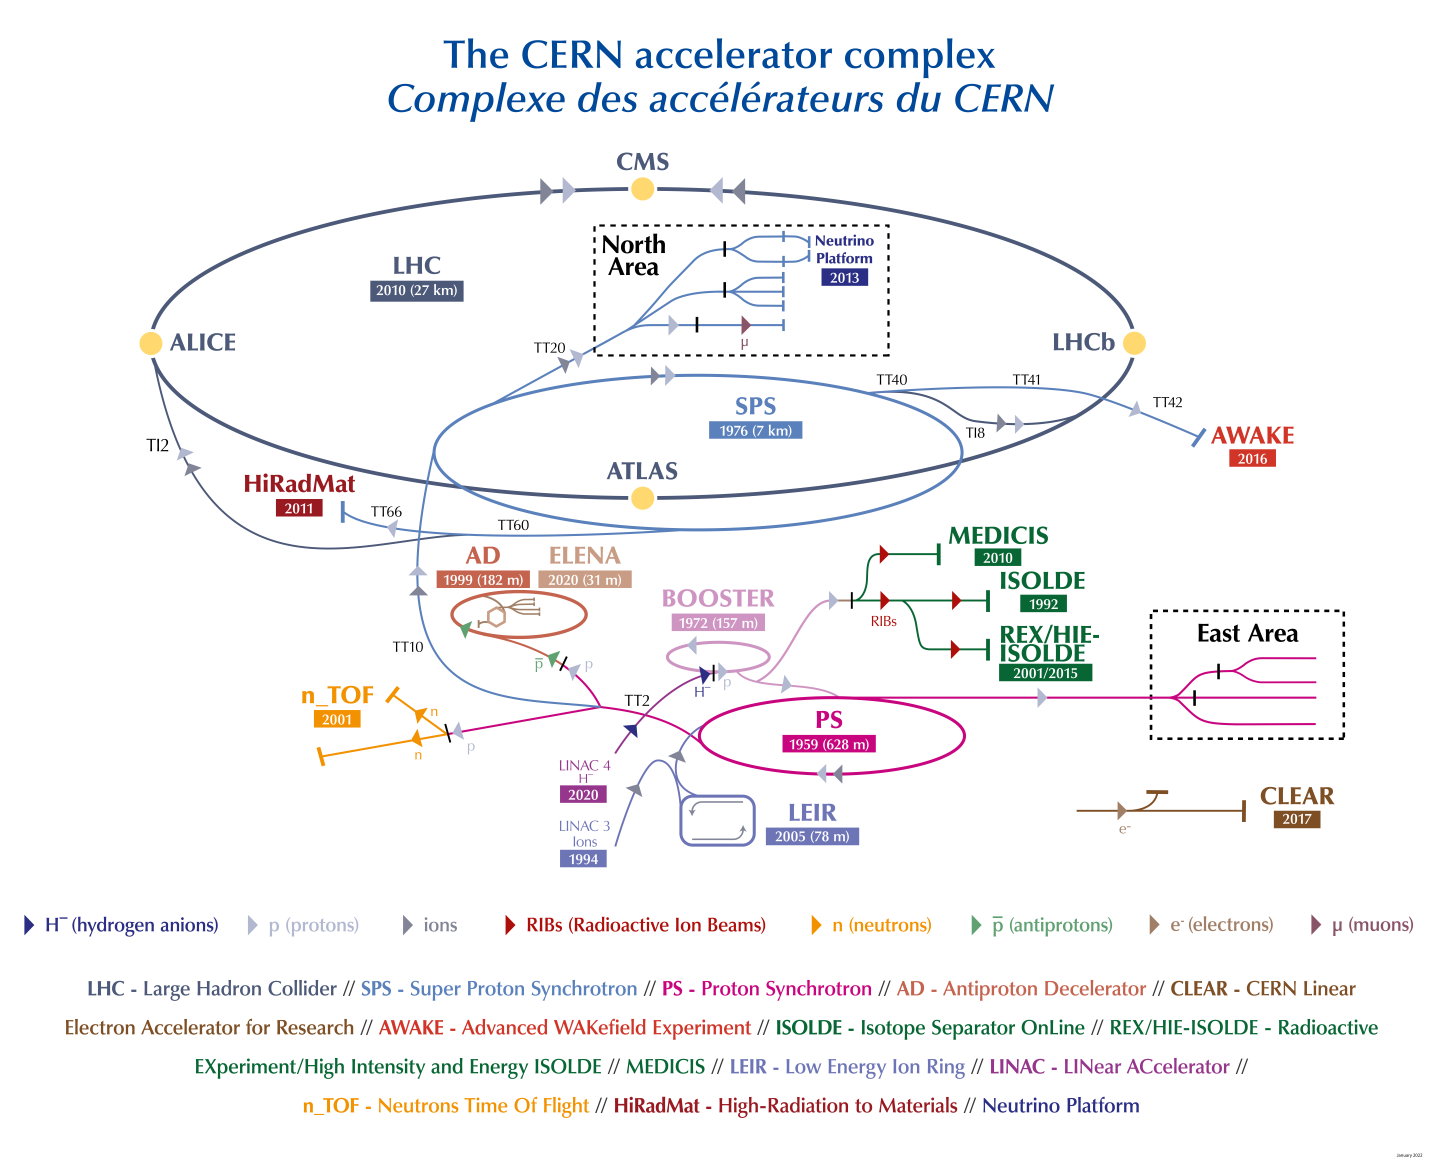
\includegraphics[width=1\textwidth]{images/cern_complex.png}
    \caption{Schematic illustration of the accelerator complex at CERN. Most accelerators are both
    used as injectors for the LHC or to provide beams to fixed target
    experiments~\cite{noauthor_cern_2022}.}
    \label{fig:introduction:cern_complex}
\end{figure}


% --------------------------------
%              LHC
% --------------------------------
\subsection{\review{The Large Hadron Collider}}

The Large Hadron Collider (LHC), is a circular particle accelerator primarily designed to collide
protons for fundamental particle physics research. It can, occasionally over the year, also collide
ions such as oxygen or lead for specifics studies. At the time of writing, in 2024, it holds several
records, such as being the largest and most powerful accelerator in the world, being near 27km long.
The LHC is composed of two beams pipes, being able to accelerate two particle beams from an
injection energy of $450$GeV to an energy of $6,800$GeV, before colliding them in four detectors:
ATLAS, CMS, Alice and LCHb.

Well publicized, the LHC is often depicted via its superconducting dipole magnets, housed in a blue
cryostat, aimed at cooling the coils. \cref{fig:3d_cut_dipole} shows a 3D cut of such magnets. The
LHC is in majority composed of those \textit{main} dipoles, as it holds $1,232$ of them, being each
about 14 meters long. Superconducting materials like Niobium-Titanium (NbTi) are utilized, as
conventional materials such as copper would melt under the current strain. There are indeed around
$12,000$ amperes supplied to generate the magnetic fields necessary for bending the trajectory of
the particles.
Those particles travel at nearly the speed of light (more precisely, $99.99999905\%$ of it),
effectively going around the tunnel about $11,200$ times per second.

\begin{figure}[!htb]
    \centering
    \includegraphics[width=0.8\textwidth]{chapters/01_Introduction/images/lhc_3D_cut.png}
    \caption{3D cut of a main LHC dipole~\cite{noauthor_cern_nodate}. Both beam pipes can be seen
    surrounded by the coils, strongly clamped by the yokes.}
    \label{fig:3d_cut_dipole}
\end{figure}


% -------------------------------
%   Straight Sections and Arcs
\subsubsection{Straight Sections and Arcs}

The LHC is not a perfect circle. It is indeed composed of four \textit{straight} sections, called
the \textit{Interaction Regions} (IPs) where detectors or specific instrumentation are placed. Connecting
those sections, the \textit{arcs} are where the majority of the magnets and their correctors are
located along with some instrument like beam position monitors.
\cref{fig:introduction:lhc_irs} shows the arcs as well as the purpose of each straight section,
housing either specific instrumentation or detectors.

\begin{figure}[!htb]
    \centering
    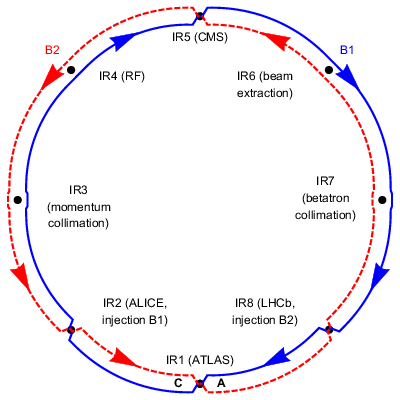
\includegraphics[width=0.5\textwidth]{./images/irs.png}
    \caption{Schematic of the LHC layout.}
    \label{fig:introduction:lhc_irs}
\end{figure}


% -------------------------------
%          Arc Cells
\subsubsection{Arc Cells}

Each arc is made up of 23 cells. Magnets are organized in a standard FoDo structure
(see \ref{section:courant_snyder}), as shows \cref{fig:introduction:lhc_arc_cell}.
\textit{Dipoles} are responsible for bending the trajectory of the particles. Their associated
correctors, the orbit correctors, mitigate any possible drift in path.
\textit{Quadrupoles} are used to control the beam size along the ring. Their effect is focusing in
one plane and defocusing in the other. Their associated correctors control the oscillations of the
beam (see tune, \ref{section:courant_snyder}) and possible field imperfections.
\textit{Sextupoles} correct chromaticity, being a misfocus from quadrupoles due to particles having
a different momentum than the reference particle.
\textit{Octupoles} are used to stabilize the beam by introducing Landau
Damping~\cite{gareyte_landau_1997}. The associated correctors correct higher order chromaticity
effects as well as amplitude dependant tune shifts.
\textit{Decapoles} correctors aim at correcting a even higher chromaticity order.

\begin{figure}[H]
    \centering
    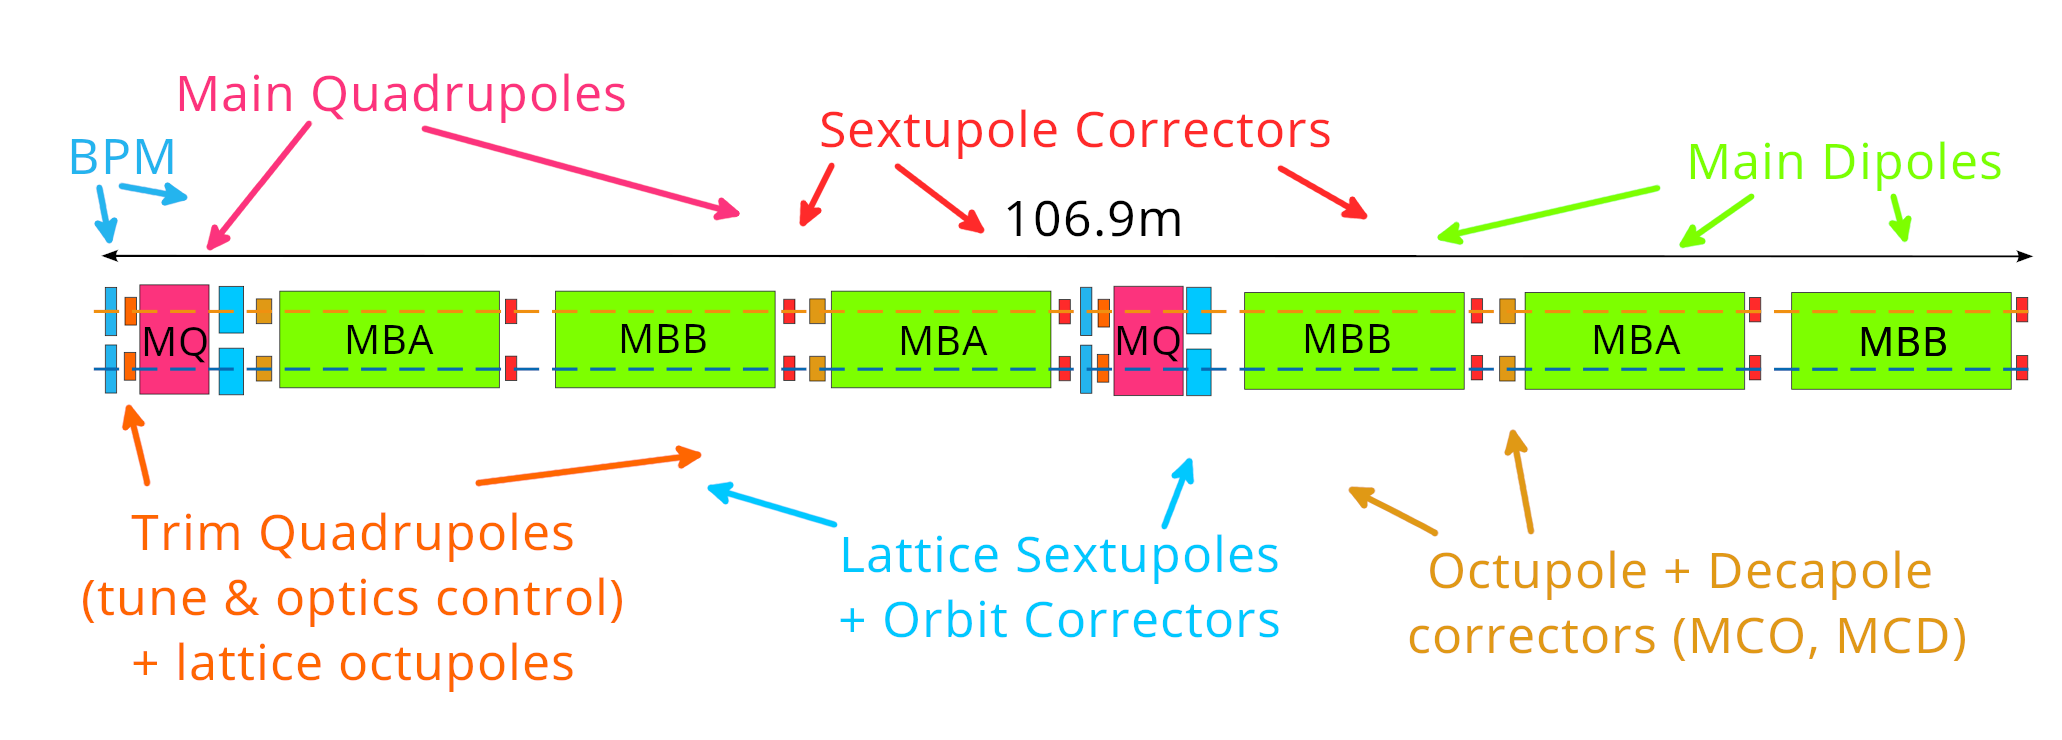
\includegraphics[width=1\textwidth]{./images/lhc_cell.png}
    \caption{Schematic of an LHC Arc cell~\cite{bruning_lhc_2004}.}
    \label{fig:introduction:lhc_arc_cell}
\end{figure}



% -------------------------------
%            Cycles
\subsubsection{\review{Cycles}}

During the operation of the LHC, the machine goes through several states. Those states of the
machine~\cite{wenniger_lhc_2019} have been defined for specific scenarios.

A common example is the operational cycle of the LHC, shown in \cref{fig:cern_complex:cycle}. The
magnets are first pre-cycled~\cite{bottura_pre-cycles_2010} without any beam circulating, to get
them back to a reproducible state. Their current is then increased to accept particles at the 
injection energy of 450GeV. In order to assess the good working condition of the machine, a probe
bunch of reduced intensity is first injected. The number of bunches and their intensity is then
ramped up to attain the desired scheme needed for collisions. This scheme varies throughout the year
depending on the demands of the experiments. The number of bunches and intensity can also be lowered
to keep the machine safe. A common scheme in 2024 is to inject about 2350 bunches with around
$10^{11}$ particles each for collisions.
Optics measurements, due to their destructive nature, typically use between one and three
\textit{pilot} bunches at a lower intensity of $10^{10}$.

The magnets current is them ramped along with the voltage injected in the RF system, to accelerate
particles to an energy of 6.8TeV. While doing so, the beam is squeezed in a first pass at the
Interaction Points. A second pass is done after the ramp is over, to reach a $\beta* = 30cm$ at the
ATLAS and CMS experiments to achieve a small beam size. Crossing-angles are then introduced to make
the beams colliding.

\begin{figure}[!htb]
    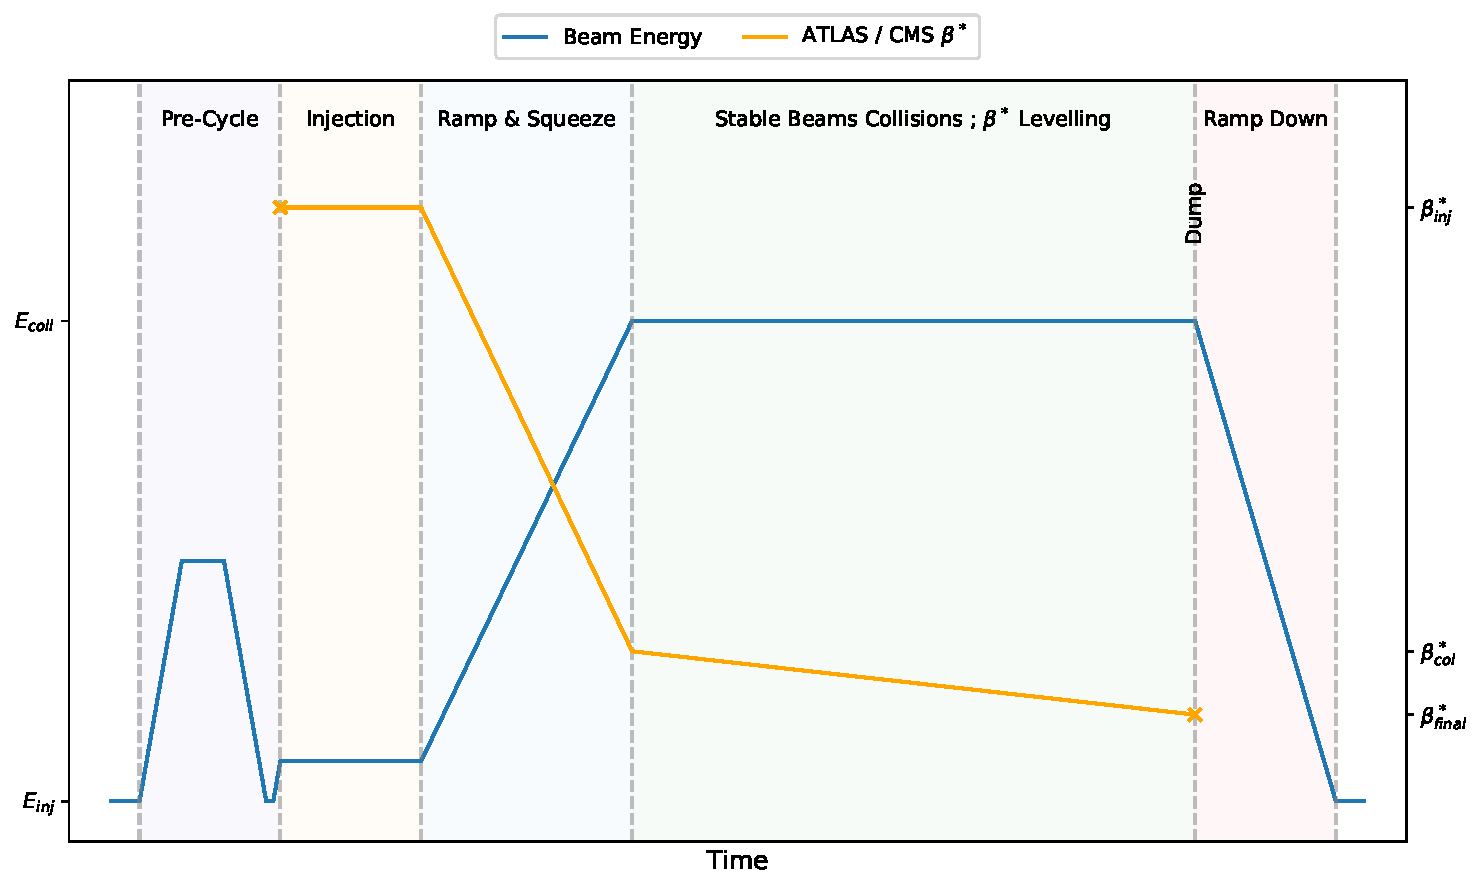
\includegraphics[width=\textwidth]{./images/lhc_cycle.pdf}
    \caption{Simplified illustration of a standard LHC cycle. Courtesy of Félix
    Soubelet~\cite{felix_soubelet_local_2023}.}
    \label{fig:cern_complex:cycle}
\end{figure}


% -------------------------------
%   Harmonics and Field Errors
\subsubsection{\review{Magnetic Fields}}

The magnetic fields of the LHC are created via the coils of the magnets. Real-life magnets never
have a single field as one would like. Instead, so called \textit{allowed harmonics} exist due to
the geometry of the coil. As such, the main dipoles of the LHC can exhibit fields similar to
sextupoles, decapoles, decatetrapoles and so on~\cite{deniau_magnetic_2009}. Manufacturing
imperfections also add fields errors outside of the scope of the allowed ones. Dipoles are indeed
found to generate octupolar field errors.

During the design of the LHC, the main dipoles have been identified to generate significant field
errors. Magnetic measurements of those various fields were thus taken and magnetic tables built
based on real-life magnets nowadays installed in the machine. Those magnetic tables, computed for
each LHC configuration by \textit{WISE}~\cite{p_hagen_wise_2006} are used by simulation softwares.
Predictions of field errors and compensating strength for the correctors is computed by the Field
Description for the LHC (\textit{FiDeL}, \cite{noauthor_fidel_2021}). FiDeL is used in the LHC
control system in operation to steer the beams.

%\begin{figure}[H]
    %\centering
    %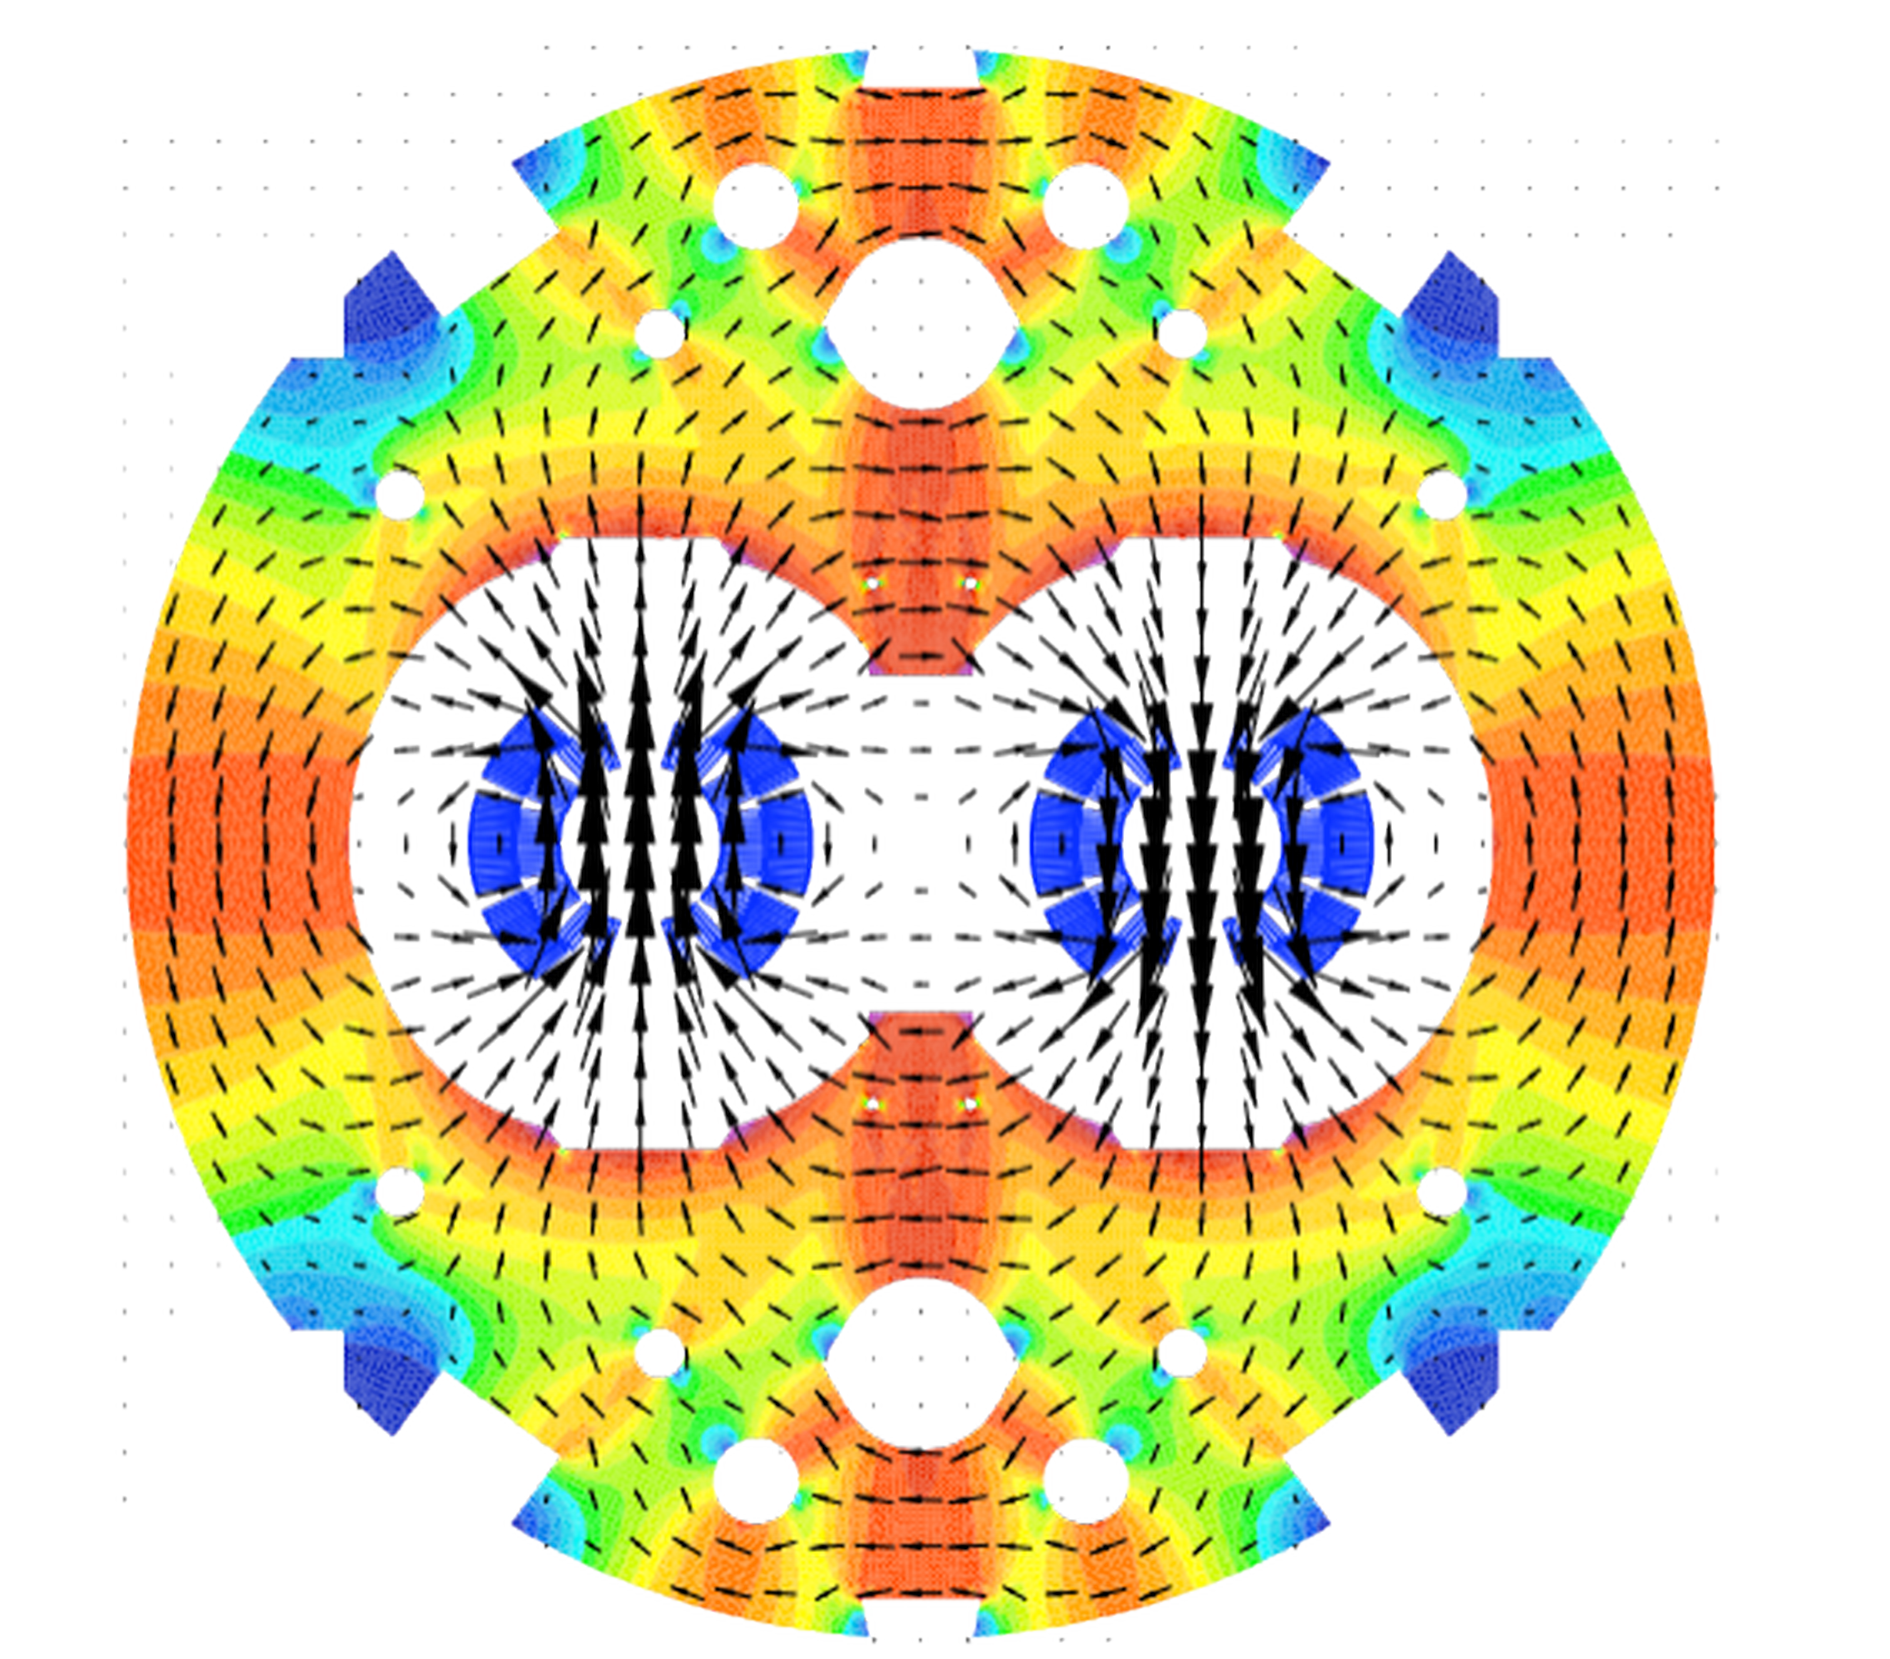
\includegraphics[width=0.5\textwidth]{./images/main_dipole_fields.png}
    %\caption{Magnetic field in a dipole magnet~\cite{deniau_magnetic_2009}.}
    %\label{fig:decapoles:magnetic_field_dipole}
%\end{figure}
\section{\review{Magnetic Fields}}

% ============================================
%                Nomenclature
% ============================================
\subsection{\review{Nomenclature}}

Several notations coexist to denote magnetic fields. In this thesis, the
\textit{European Convention}~\cite{dilly_corrections_2022} is used for field indices, as shown
in Tab.~\ref{tab:magnetic_fields:relation_indices}. MAD-X, and MAD-NG, however, use the
\textit{American Convention}.

\begin{table}[H]
    \centering
    \begin{tabular}{lccc}
    \toprule
        Multipole     &     Index        & Normalized Strength  &      MAD-X      \\
    \midrule                                                    
        Dipole        &     1            & $K_1$                &     0           \\
        Quadrupole    &     2            & $K_2 $               &     1           \\
        Sextupole     &     3            & $K_3 $               &     2           \\
        Octupole      &     4            & $K_4 $               &     3           \\
        Decapole      &     5            & $K_5 $               &     4           \\
        Dodecapole    &     6            & $K_6 $               &     5           \\
        Decatetrapole &     7            & $K_7 $               &     6           \\
        Decahexapole  &     8            & $K_8 $               &     7           \\
    \bottomrule
    \end{tabular}
    \caption{Relation between field indices and multipoles.}
    \label{tab:magnetic_fields:relation_indices}
  \end{table}

As such, unless explicitly stated, quantities such as the magnetic strength $b$ and normalized
strength $K$ will be expressed with this notation. 


% ============================================
%              Multipole Expansion
% ============================================
\subsection{\review{Multipole Expansion}}

A 2 dimension magnetic field in the planes \textit{x} and \textit{y} can be described as a sum of
the normal and skew field gradients $\mathcal{B}$ and $\mathcal{A}$ with multipoles of order $n$,
given by~\cite{wolf_engineering_2001}:
\begin{equation}
    B_y + iB_x = \sum_{n=1}^\infty \left(\mathcal{B}_n + i\mathcal{A}_n \right)  (x+iy)^{n-1}
\end{equation}

An ideal magnet would produce either a sole normal or skew field. However, this is not applicable 
to real-life magnets that are imperfect, due to design and manufacturing constraints.
Field errors are thus introduced, relative to the main field of the ideal 2N-pole magnet at a
reference radius $r_{ref}$~\cite{dilly_corrections_2022}, as shown in 
Eq.~\eqref{eq:magnetic_field:relative_errors}. The coefficients of the normal and skew relative 
field errors, referred to as $a_n$ and $b_n$, are dimensionless but often given in \textit{units}
of $10^{-4}$.

\begin{equation}
    B_y + iB_x = 
        \begin{cases}
            \mathcal{B}_N \cdot \sum_{n+1}^\infty (b_n + ia_n) \left(\frac{x+iy}{r_{ref}}\right)^{n-1}\text{, for normal magnets}\\
            \mathcal{A}_N \cdot \sum_{n+1}^\infty (b_n + ia_n) \left(\frac{x+iy}{r_{ref}}\right)^{n-1}\text{, for skew magnets}
        \end{cases}
    \label{eq:magnetic_field:relative_errors}
\end{equation}


The normal and skew field components of order $n$ for an imperfect 2N-pole magnet is thus given by
the following equation:

\begin{equation}
    \begin{aligned}
        \mathcal{B}_n &= \mathcal{B}_N \cdot \frac{b_n}{r_{ref}^{n-1}}, \\
        \mathcal{A}_n &= \mathcal{A}_N \cdot \frac{a_n}{r_{ref}^{n-1}}.
    \end{aligned}
\end{equation}

The unit of the field is relative to the multipole order $n$: $[\text{Tm}^{1-n}]$.


% ============================================
%              Normalization
% ============================================
\subsection{\review{Beam Rigidity and Normalization}}

\subsubsection{\review{Beam Rigidity}}

The beam rigidity refers to the resistance of a particle moving through the accelerator to the
bending applied by the magnetic fields. It is derived from the Laurentz force~\cite{dilly_corrections_2022}
and relates the magnetic field $B$, the radius of curvature $\rho$ to the momentum $p$ and charge $q$
of the particle:

\begin{equation}
    B \rho = \frac{p}{q}
    \label{eq:magnetic_fields_beam_rigidity}
\end{equation}

It is of interest when designing an accelerator to set the maximum field as well as the required
radius of curvature for a specific momentum and particle.
An interesting metric of an accelerator is also its \textit{filling factor}, or percentage of
dipoles in the machine. It can be calculated via the radius of curvature: $f = \rho / r$. A low 
filling factors means more space for other magnets, collimators, beam instrumentation, etc.

\subsubsection{\review{Field Normalization}}

The Beam Rigidity is also used as a way to normalize magnetic field strengths in particle
accelerators where the momentum of the particle changes (i.e. acceleration).
Normalized Normal and Skew components $K_n$ and $J_n$ are given by~\cite{wolf_engineering_2001}:

\begin{equation}
    \begin{aligned}
        K_n =  \frac{q}{p} &(n-1)! \mathcal{B}_n, \\ 
        J_n =  \frac{q}{p} &(n-1)! \mathcal{A}_n.
    \end{aligned}
    \label{eq:magnetic_fields_normalized}
\end{equation}



% ============================================
%            Hamiltonian Dynamics
% ============================================
\subsection{\review{Hamiltonian}}

The Hamiltonian describing the motion for the transverse planes of a given multipole or order $n$ is
given by~\cite{keintzel_jacqueline_beam_nodate,tomas_direct_2003,franchi_studies_2006}:

\begin{equation}
    \begin{aligned}
        H &= \frac{q}{p} \Re \left[ \sum_{n>1} (\mathcal{B}_n + i\mathcal{A}_n) \frac{(x+iy)^n}{n} \right] \\
          &= \Re \left[ \sum_{n>1} (K_n + iJ_n) \frac{(x+iy)^n}{n!} \right].
    \end{aligned}
    \label{eq:hamiltonian_magnet}
\end{equation}

Quite often, when studying the effect of a magnet on the beam, only one component is required, and
the sum can thus be dropped.
The normal and skew fields can also be isolated in order to consider their effect only:

\begin{equation}
    \begin{aligned}
        N_n &= \frac{1}{n!} K_n \Re \left[ (x+iy)^n \right] \\
        S_n &= -\frac{1}{n!} J_n \Im \left[ (x+iy)^n \right].
    \end{aligned}
    \label{eq:normal_skew_hamiltonian_magnet}
\end{equation}




\section{\review{Coordinate Systems}}

In circular accelerators, particle dynamics are represented using a traveling coordinate system.
A reference orbit is determined by the lattice and its magnet strengths, forming the
\textit{optics}. In the case of a synchrotron, like the LHC, the reference orbit is also called the
closed orbit.

The Frenet-Serret coordinate system moves along the ring on the reference orbit. The coordinates are
then transverse: $x$ and $y$, and longitudinal in the direction of travel: $s$.
\Cref{fig:coordinate_systems:frenet_serret} shows those coordinates.

\begin{figure}[H]
    \centering
    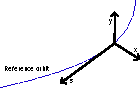
\includegraphics[width=0.5\textwidth]{images/frenet.pdf}
    \caption{Frenet-Serret coordinate system, commonly used in accelerator physics. The system moves
    along the reference orbit.}
    \label{fig:coordinate_systems:frenet_serret}
\end{figure}

This coordinate system is widely used to simply describe a either an element's or a particle's
position in the accelerator. Without any explicit mention, those are coordinates used in this
thesis. It is frequent to use the variable $z$ to refer to either $x$ or $y$ in equations.
In order to describe the motion of particles through a lattice, different coordinate systems can be
used. To better describe the motion of particles through a lattice, various coordinate systems can
be employed. First, the formalism for a linear lattice will be introduced, followed by an
explanation of how motion in a machine with non-linear elements can be characterized.

Linear optics refers to the regime where the forces acting on particles, such as those from dipoles
and quadrupoles, are directly proportional to the particle's displacement from the reference
trajectory, resulting in simple, predictable motion described by linear equations and transfer
matrices. Non-linear optics, on the other hand, involves higher-order magnetic elements like
sextupoles and octupoles, where the forces are non-linear with respect to displacement. This leads
to more complex particle motion, which can result in phase-space distortions and chaotic
trajectories.


% ============================================
%               Linear Lattice 
% ============================================
\subsection{\review{Linear Lattice}}

% ========================
% Courant-Snyder Parameters
\subsubsection{\review{Courant-Snyder Parameters}}
\label{section:courant_snyder}

A circular accelerator is composed of many multipoles of different orders. A very basic
design only requires dipoles and quadrupoles in order to operate. Dipoles are used to bend the
particles in order to form the ring, whereas quadrupoles are used to focus the beam to a focal
point, similar to light optics.
Those elements can be arranged in a particular order, to form a FoDo cell. Such cells present an
alternating placement of focusing an defocusing quadrupoles with dipoles in between, as shown in
\cref{fig:coordinate_systems:fodo}, and are usually repeated many times along the ring.

\begin{figure}[htb]
    \centering
    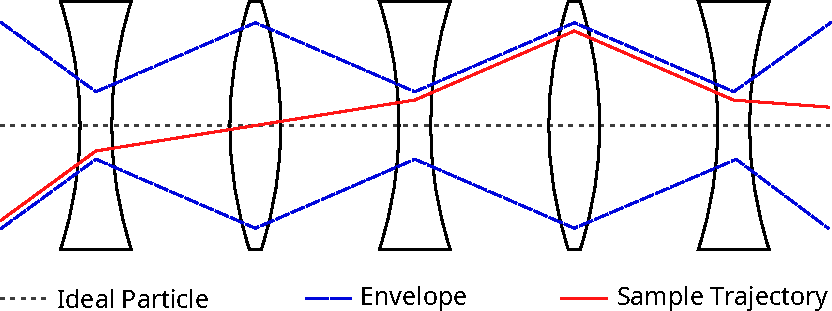
\includegraphics[width=0.8\textwidth]{images/fodo_drawing.pdf}
    \caption{Line composed of FoDo cells, a basic cell present in most accelerators, composed of a
    Focusing and a Defocusing quadrupole. The envelope is a factor of the $\beta$-function and the
    action $J$.}
    \label{fig:coordinate_systems:fodo}
\end{figure}

A lattice composed of only dipoles and quadrupoles, is referred to as a \textit{linear} lattice.  In
a synchrotron, a circular particle accelerator, particles undergo transverse and longitudinal 
oscillations. Taking into account those oscillations, the phase-space ellipse of a particle at a 
position $s$ in the ring can be described with a new system: the Courant-Snyder parameters, also
know as Twiss parameters or the \textit{optics functions}~\cite{courant_theory_1958}, as shown in
\cref{fig:coordinate_systems:twiss}.

\begin{figure}[htb]
    \centering
    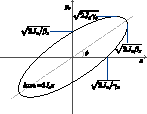
\includegraphics[width=0.6\textwidth]{images/phase_space.pdf}
    \caption{Phase-space ellipse of a linear machine, parametrized by the Courant-Snyder
    parameters $\alpha$, $\beta$ and $\gamma$.}
    \label{fig:coordinate_systems:twiss}
\end{figure}

$J$, the action, is invariant of linear motion at a given energy and describes the amplitude of 
oscillations. It is related to the other quantities by:

\begin{equation}
    J_z = \frac{1}{2} (\gamma_z \cdot z^2 + 2 \alpha_z p_z \cdot z + \beta_z p_z^2).
    \label{eq:coordinate_systems:action}
\end{equation}

The action can be related to the area in phase space, called the single particle emittance:
$\epsilon = 2J$.  As the $\beta$ parameter varies along the ring, it is referred to as the
$\beta$-function and is related to the amplitude of the oscillations. Thus, the smaller is the
$\beta$-function, the smaller is also the envelope of the beam.
The number of oscillations per turn is called the \textit{tune}, and is closely related to the
$\beta$-function:

\begin{equation}
    Q_{x,y} = \frac{1}{2 \pi} \oint \frac{1}{\beta_{x,y}(s)} \diff s.
    \label{eq:coordinate_systems:tune}
\end{equation}


It is common to express the position of a particle using \textit{action-angle} variables, allowing
to switch between the Courant-Snyder parameters and the Frenet-Serret system:

\begin{equation}
    \begin{aligned}
    z   &= \sqrt{2J_z \beta_z} \cos{\phi_z} \\
    p_z &= - \sqrt{\frac{2J_z}{\beta_z}} \left( sin{\phi_z} + \alpha_z \cos{\phi_z}\right).
    \end{aligned}
    \label{eq:coordinate_systems:action_angle}
\end{equation}


\subsubsection{\review{Normalized Coordinates}}

In order to simplify the description of the linear motion in a ring, a transformation can be applied
to the previously seen coordinates. Figure \cref{fig:coordinate_systems:normalized_coordinates}
shows a phase-space described in both coordinates. The new coordinates, $\hat{z}$, and $\hat{p}_z$,
are then expressed as factors of the $\alpha$ and $\beta$ functions:

\begin{equation}
    \begin{pmatrix}
        \hat{z}    \\
        \hat{p}_z 
    \end{pmatrix}
    =
    \begin{pmatrix}
        \frac{1}{\sqrt{\beta_z}}         &   0 \\
        \frac{\alpha_z}{\sqrt{\beta_z}}  &   \sqrt{\beta_z}
    \end{pmatrix}
    \begin{pmatrix}
        z \\
        p_z 
    \end{pmatrix}.
\end{equation}

This allows to describe the motion as a simple rotation, the new coordinates being only dependent on
the invariant $J_z$ and the phase $\phi_z$:

\begin{equation}
    \begin{aligned}
        \hat{z}   &= \sqrt{2J_z} \cos \left(\phi_z \right), \\
        \hat{p}_z &= \sqrt{2J_z} \cos \left(\phi_z \right).
    \end{aligned}
\end{equation}     

\begin{figure}[H]
    \centering
    \begin{subfigure}[b]{0.4\textwidth}
        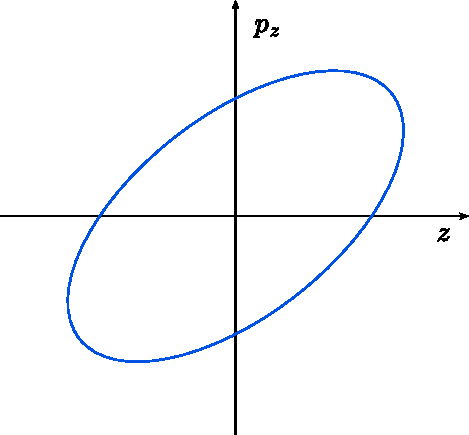
\includegraphics[width=\linewidth]{images/phase_space_regular_coordinates.pdf}
        %\caption{Caption for Image 1}
        %\label{fig:sub1}
    \end{subfigure}
    \begin{subfigure}[b]{0.4\textwidth}
        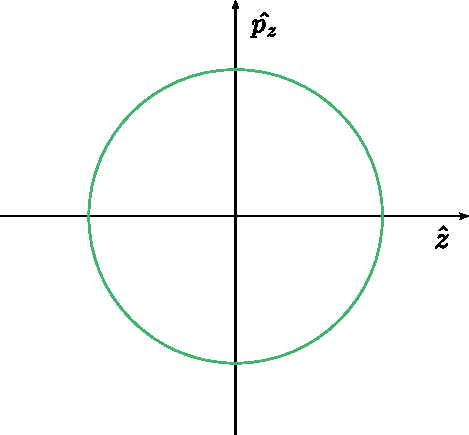
\includegraphics[width=\linewidth]{images/phase_space_normalized_coordinates.pdf}
        %\caption{Caption for Image 2}
        %\label{fig:sub2}
    \end{subfigure}
    \caption{Phase space described in both regular and normalized coordinates}
    \label{fig:coordinate_systems:normalized_coordinates}
\end{figure}


% ========================
% Linear Transfer Map
\subsubsection{\review{Linear Transfer Maps}}
\label{section:coordinate_systems:linear_maps}

The final position of a particle after passing through an accelerator element can be described using
\textit{transfer maps}. In the case of linear optics, these maps take the form of matrices.
Importantly, these maps should be symplectic, meaning they preserve the area of phase space,
ensuring that the particle's motion is accurately represented. Symplecticity guarantees that key
properties of the beam, such as its emittance, remain consistent, which is crucial for maintaining
the stability and integrity of particle trajectories in the accelerator.
For a matrix $\mathcal{M}$ and positions $z$ at the initial location and $s$, the general formula
reads~\cite{lee_accelerator_2004}:

\begin{equation}
    \begin{pmatrix}
        z \\
        z'
    \end{pmatrix}_s
    = M \cdot 
    \begin{pmatrix}
        z \\
        z'
    \end{pmatrix}_0
\end{equation}

This formalism assumes that the magnetic field is constant along the element in the longitudinal
direction. Basic elements such as drifts, dipoles, quadrupoles can then be described be a simple
$2 \times 2$ matrix:

\begin{equation}
    M_{drift} = \begin{pmatrix}
                    1 & L \\
                    0 & 1 
                \end{pmatrix},
\end{equation}
\begin{equation}
    M_{dipole} = \begin{pmatrix}
                    \cos\left(L/\rho\right) & \rho \sin\left(L/\rho\right) \\
                    -1/\rho \sin\left(L/\rho\right) & \cos\left(L/\rho\right)
                 \end{pmatrix}, \\
\end{equation}
\begin{equation}
    M_{focusing\;quad.} = \begin{pmatrix}
                             \cos\left(\sqrt{k_2}L\right) & 1/\sqrt{k_2} \sin\left(\sqrt{k_2}L\right) \\
                             -\sqrt{k_2}\sin\left(\sqrt{k_2}L\right) & \cos\left(\sqrt{k_2}L\right)
                          \end{pmatrix},\\
\end{equation}
\begin{equation}
    M_{defocusing\;quad.} = \begin{pmatrix}
                        cosh\left(\sqrt{|k_2|}L \right) & 1/\sqrt{|k_2|} sinh\left(\sqrt{|k_2|} L\right) \\
                        \sqrt{|k_2|} sinh\left(\sqrt{|k_2|} L\right) & cosh\left(\sqrt{|k_2|} L \right)
                            \end{pmatrix},\\
\end{equation}

where L is the length of the element, $\rho$ the radius of curvature of the orbit and $k_2$ the
normalized strength of quadrupoles. In the case of quadrupoles, a focusing matrix should be used in
the horizontal plane for focusing quadrupoles, where defocusing matrices should be used in the
vertical plane. The opposite goes for defocusing quadrupoles.

Transfer matrices can be combined together to describe a larger group of elements, as the FoDo cell
seen previously. Its transfer matrix can then be expressed as:

\begin{equation}
    M_{FoDo} = M_{focusing\;quad} \cdot M_{drift} \cdot M_{defocusing\;quad} \cdot M_{drift}.
\end{equation}

For a closed machine, a full revolution can be described by a so-called \textit{one-turn map}, being
the transfer matrix of the whole machine, denoted $\mathcal{M}$. Such a map can potentially contain
thousands of elements.


% ============================================
%             Non-Linear Lattice 
% ============================================
\subsection{\review{Non-Linear Lattice}}

So far, Courant-Snyder parameters were a good way to describe the distribution of positions and
velocities of particles in the transverse plane. One caveat of using this formalism is that it is 
restrained to linear optics and does not address non-linear elements, like octupoles. These elements
generate forces that are not directly proportional to a particle's displacement from the reference
trajectory.
Effects such as resonances or those arising from an arrangement of several multipoles together can
be described by the concepts introduced in this section.
An overview of the needed mathematical tools is first given, before introducing maps.

% ========================
% Lie Algebra
\subsubsection{\review{Lie Algebra}}

One way to describe non-linear effects is to introduce Lie Algebra~\cite{dragt_overview_2013}, a
powerful algebra able to describe transformations, symmetries and their associated conserved
quantities. 
The Lie algebra is a vector space, denoted $\mathfrak{g}$, equipped with a binary operation called
the \textit{Lie bracket} and denoted $[x, y]$ for two vectors $x$ and $y$. Any vector space equipped
with a Lie bracket (or commutator) satisfying the following conditions is called a Lie
algebra:

\begin{itemize}
    \item Bilinearity:
    \begin{equation}
        \begin{aligned}
        \relax[ax+by, z] &= a[x,z] + b[y,z], \\
        [z, ax+by] &= a[z,x] + b[z,y], \quad \forall x,y,z \in \mathfrak{g}~\text{and}~a,b~\text{scalars}
        \label{eq:coordinates:bilinearity}
        \end{aligned}
    \end{equation}

    \item Alternativity:
    \begin{equation}
        [x,x] = 0, \quad \forall x \in \mathfrak{g}
    \end{equation}

    \item Anticommutativity:
    \begin{equation}
        [x,y] = -[y,x], \quad \forall x,y \in \mathfrak{g}
    \end{equation}

    \item The Jacobi identity:
    \begin{equation}
        [x,[y,z]] + [y, [z,x]] + [z, [x,y]] = 0, \quad \forall x,y,z \in \mathfrak{g}
        \label{eq:coordinates:jacobi_identity}
    \end{equation}
\end{itemize}

The \textit{Lie bracket}, plays a central role in the Lie algebra. It describes how dynamical
variables evolve under infinitesimal symplectic transformations.


% ========================
% Poisson Brackets
\subsubsection{\review{Poisson Brackets}}

In accelerator physics, following the Hamiltonian formalism and classical mechanics, the commutator
is represented by the \textit{Poisson brackets}, which satisfy the necessary conditions for
describing particle motion~\cite{dragt_overview_2013,roy_analysis_1992}. Poisson brackets are used
to express continuous symmetries, conserved quantities, and the time evolution of dynamical
variables within the system. 

Let's consider position and momentum coordinates $q_i \cdots q_n$ and $p_i \cdots p_n$  of a
2n-dimensional phase space. Usually, those would be $x, y, p_x \text{ and } p_y$ for transverse
coordinates. The Poisson brackets of two functions $f$ and $g$ is then defined by:

\begin{equation}
    [f,g] = \sum^n_{i=1} \frac{\partial f}{\partial q_i} \frac{\partial g}{\partial p_i}
                       - \frac{\partial f}{\partial p_i} \frac{\partial g}{\partial q_i}.
    \label{eq:coordinate_systems:poisson_bracket}
\end{equation}


The evolution of coordinates and momenta in time is described by Hamilton's equations of motion, which can
be naturally expressed with Poisson brackets:

\begin{equation}
    \begin{aligned}
        \frac{\partial H}{\partial p_i}   &= \frac{\diff q_i}{\diff t}  &&= [q_i, H] \\
       -\frac{\partial H}{\partial q_i}   &= \frac{\diff p_i}{\diff t}  &&= [p_i, H].
    \end{aligned}
\end{equation}


% ========================
% Lie Operator
\subsubsection{\review{Lie Operator}}

Given a function $f$, a differential operator called \textit{Lie operator} is defined, and is closely
related to the previously seen Poisson bracket:

\begin{equation}
:f: = \sum^n_{i=1} \frac{\partial f}{\partial q_i} \frac{\partial}{\partial p_i}
                    - \frac{\partial f}{\partial p_i} \frac{\partial}{\partial q_i}.
\end{equation}

The action of this operator on a function $g$ is equivalent to the Poisson brackets, as in:

\begin{equation}
    :f:g = [f,g].
\end{equation}

A particular power series of this Lie operator can now be defined, called \textit{Lie
transformation}:

\begin{equation}
    \begin{aligned}
        e^{:f:}g &= \sum_{l=0}^\infty \frac{1}{l!} :f:^l g \\
                 &= g + [f,g] + \frac{1}{2!}[f, [f, g]] + \cdots .
    \end{aligned}
    \label{eq:coordinate_systems:expansion_exponential}
\end{equation}



% ========================
% Non-Linear Transfer Map
\subsubsection{\review{Non-Linear Transfer Maps}}

As introduced in \cref{section:coordinate_systems:linear_maps}, the dynamics of a particle beam in a
circular accelerator can be described by \textit{transfer maps}. A symplectic \textit{One Turn Map}
$\mathcal{M}$ that includes $N$ non-linear elements is defined~\cite{dragt_overview_2013} as:

\begin{equation}
    \mathcal{M} = e^{:h_N:} \cdot e^{:h_{N-1}:} \cdots e^{:h_1:} \cdot \mathcal{R}
\end{equation}

where $\mathcal{R}$ is a matrix describing the linear motion over one turn and the $h_i$ terms
representing the Hamiltonian of each non-linear elements of the machine.
Via the Baker-Campbell-Hausdorff (BCH) theorem~\cite{forest_beam_1998,casas_efficient_2009},
previous Lie transformations can be combined and simplified via
\cref{eq:coordinates:basic_exponent_bch} and \cref{eq:coordinates:bch}. Further orders can be found
and computed via~\cite{casas_efficient_2009}.

\begin{equation}
    e^{:h_1:} \cdot e^{:h_2:} = e^{:h:}
    \label{eq:coordinates:basic_exponent_bch}
\end{equation}
with 
\begin{equation}
    \begin{alignedat}{3}
      h =& h_1 + h_2  && \Rightarrow \text{1\textsuperscript{st} order}\\
             & + \frac{1}{2} [h_1, h_2]  && \Rightarrow \text{2 \textsuperscript{nd} order}\\
             & + \frac{1}{12} [h_1, [h_1, h_2]] - \frac{1}{12} [h_2, [h_1, h_2]] \quad && \Rightarrow \text{3\textsuperscript{rd} order}\\
             & + \cdots.
    \end{alignedat}
    \label{eq:coordinates:bch}
\end{equation}


The one turn map is thus expressed as a single Lie transformation:

\begin{equation}
    \mathcal{M} = e^{:h:} \cdot \mathcal{R}.
   \label{eq:coordinate_systems:non_linear_map}
\end{equation}

In most cases, where the non-linear perturbations are small, the above series converges quickly
and only the first order of \cref{eq:coordinates:bch} is
used~\cite{carlier_nonlinear_2020-1}. The resulting expression is then more elegant, being a simple
sum of the Hamiltonians of the $N$ non-linear elements:

\begin{equation}
   \mathcal{M} = e^{:h_1 + h_2 + \cdots + h_N:} \cdot \mathcal{R}.
\end{equation}

It is though to be noted that in this thesis experimental measurements show the evidence of higher
order contributions. In order to fully understand the combined effect of multipoles, the BCH
expansion needs to be expended further than the first two terms.

When transporting coordinates from one point to another, the length of the elements must be taken
into account:

\begin{equation}
    \begin{aligned}
        e^{:LH:} x_0 &= x_1,\\
        e^{:LH:} p_0 &= p_1.
    \end{aligned}
\end{equation}


% ========================
% Normal Form
\subsubsection{\review{Normal Form}}

As non-linearities are introduced in the machine, the phase-space becomes distorted, resulting in
$J_z$ no longer being an invariant of motion. The previously seen normalization does not work
anymore and the phase-space is no longer a simple circle. A new normalization is then introduced,
called the \textit{normal form}, with complex coordinates $\zeta$, depending on new action and
angle coordinates $I_z$ and $\psi_z$:

\begin{equation}
    \zeta_{z,\pm} = \sqrt{2I_z} e^{\mp i \psi_z}.
    \label{eq:coordinate_systems:normal_form_coordinates}
\end{equation}

An exaggerated vision of such a phase-space in Courant-Snyder, normalized, and normal form
coordinates can be seen in \cref{fig:coordinate_systems:distorted_phase_space}.

\begin{figure}[H]
    \centering
    \begin{subfigure}[b]{0.292\textwidth}
        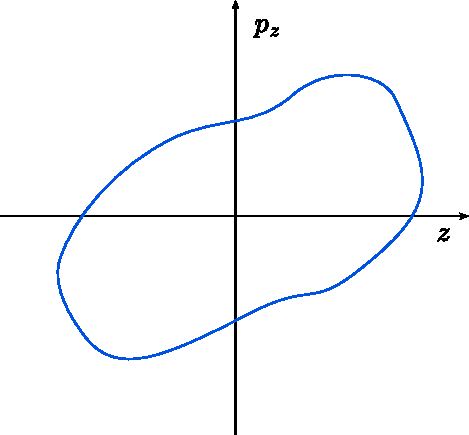
\includegraphics[width=\linewidth]{images/phase_space_regular_coordinates_wonky.pdf}
        %\caption{Caption for Image 1}
        %\label{fig:sub1}
    \end{subfigure}
    \begin{subfigure}[b]{0.292\textwidth}
        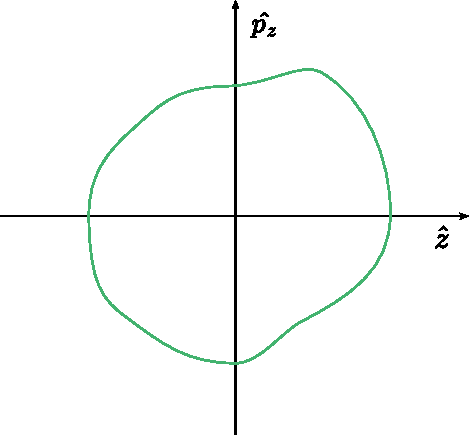
\includegraphics[width=\linewidth]{images/phase_space_normalized_coordinates_wonky.pdf}
    \end{subfigure}
    \begin{subfigure}[b]{0.316\textwidth}
        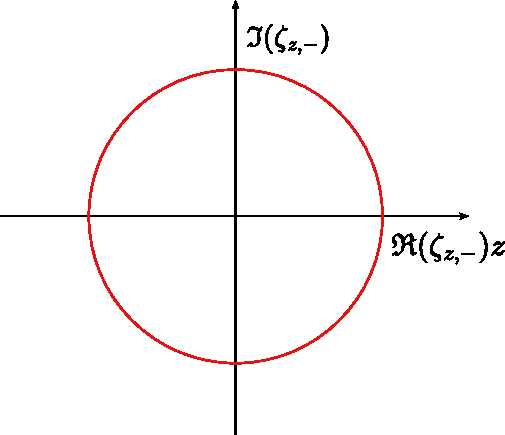
\includegraphics[width=\linewidth]{images/phase_space_normal_form_coordinates.pdf}
    \end{subfigure}
    \caption{Exaggerated phase space distorted by non-linearities described in regular (left),
    normalized (middle) and normal form (right) coordinates.}
    \label{fig:coordinate_systems:distorted_phase_space}
\end{figure}

The map defined previously in \cref{eq:coordinate_systems:non_linear_map} can be rewritten in order
to retrieve an invariant of motion $I_z$ by introducing a generating function $F$:

\begin{equation}
    \tilde{\mathcal{M}} = e^{:-F:} \mathcal{M} e^{:F:}
    \label{eq:coordinate_systems:non_linear_map_normal_form}
\end{equation}



Such a generating function includes all the non-linearities, simplifying the calculations.
Going back and forth from normalized to normal forms coordinates is then straightforward, as
depicted in \cref{fig:coordinate_systems:non_linear_map_normal_form}. The hamiltonian $H$ is now
only dependent on the action $I_z$.


\begin{figure}[H]
    \centering
    \begin{tikzpicture}[>=stealth]
        % Defining the coordinates
        \coordinate (A) at (0, 0);
        \coordinate (B) at (0, 2);
        \coordinate (C) at (3, 0);
        \coordinate (D) at (3, 2);
        
        % Drawing lines with arrows
        \draw[shorten <=0.2cm, shorten >=0.2cm, ->] (B) -- node[left, text centered] {$e^{:-F:}$} (A);
        \draw[shorten <=0.2cm, shorten >=0.2cm, ->] (C) -- node[right, text centered] {$e^{:F:}$} (D);
        \draw[shorten <=0.4cm, shorten >=0.5cm, ->] (A) -- node[below, text centered] {$e^{:H:} \cdot \mathcal{R}$} (C);
        \draw[shorten <=0.9cm, shorten >=1.1cm, ->] (B) -- node[above, text centered] {$\hat{\mathcal{M}}$} (D);
        
        % Adding labels
        \node at (B) []{$(\hat{z} \pm i\hat{p}_z)_N$};
        \node at (D) []{$(\hat{z} \pm i\hat{p}_z)_{N+1}$};
        \node at (C) [] {$\zeta_{N+1}$};
        \node at (A) [] {$\zeta_{N}$};
    \end{tikzpicture}
    \caption{A one turn map from turn N to N+1 solved using a generating function $F$, 
    transforming to normal form coordinates $\zeta$, applying the linear rotation $R$ and
    transforming back to normalized coordinates.}
    \label{fig:coordinate_systems:non_linear_map_normal_form}
\end{figure}

The function $F$ is defined as

\begin{equation}
    F = \sum_{jklm} f_{jklm}\zeta_{x,+}^j \zeta_{x,-}^k \zeta_{y,+}^l \zeta_{y,-}^m,
\end{equation}

where $f_{jklm}$ are the so-called Resonance Driving Terms (RDTs).  The summation $jklm$ is done
over all the combinations of $j$, $k$, $l$ and $m$ with $j+k+l+m = n$ for a multipole of order $n$,
as shown in \cref{eq:coordinates_systems:sum_jklm}:

\begin{equation}
    \sum_{jklm} = \sum_{j=0}^n \sum_{k=0}^n \sum_{l=0}^n \sum_{m=0}^n \quad;\quad j+k+l+m=n.
    \label{eq:coordinates_systems:sum_jklm}
\end{equation}

The expression of the resonance driving terms is given by the global hamiltonian term $h_jklm$ by

\begin{equation}
    f_{jklm} = \frac{h_{jklm}}{1 - e^{i2\pi \left[ (j-k)Q_x + (l-m) Q_y \right]}},
    \label{eq:coordinate_systems:fjklm}
\end{equation}

where this coefficient is a summation over the hamiltonian terms of elements $w$ in the lattice,

\begin{equation}
    h_{jklm} = \sum_w h_{w,jklm} e^{i [(j-k)\Delta \phi_x + (l-m) \Delta \phi_y]}.
\end{equation}

The expression of $h_{w,jklm}$ is itself derived from the general hamiltonian 
of \cref{eq:hamiltonian_magnet} by applying a multinomial expansion on the
coordinates~\cite{franchi_studies_2006} as shows \cref{eq:coordinate_systems:hwjklm}.
Derivations and more information on resonance driving terms can be found in \cref{appendix:rdts}.

\begin{equation}
    h_{w,jklm} = -\Re \left[\frac{K_{w,n} + iJ_{w,n}}{j!k!l!m! 2^{j+k+l+m}}
    i^{l+m} \beta_{w,x}^{\frac{j+k}{2}} \beta_{w,y}^{\frac{l+m}{2}} \right]
    \label{eq:coordinate_systems:hwjklm}
\end{equation}

Transforming from the normal form coordinates back to the original normalized coordinates can be
done using the right side of \cref{fig:coordinate_systems:non_linear_map_normal_form}. Which is
written, to second order, as:

\begin{equation}
    \begin{aligned}
        h_z^{ \pm} &= e^{: F:} \cdot \zeta_z^{ \pm} \\
                   &\simeq \zeta_z^{ \pm}+\left[F, \zeta_z^{ \pm}\right] 
                        + \frac{1}{2!} \left[ F, \left[ F, \zeta_z^\pm \right]\right].
    \end{aligned}
\end{equation}

Using this equation to the first order and \cref{eq:coordinate_systems:normal_form_coordinates}, the
normalized coordinates can be expressed after $N$ turns in
\cref{eq:coordinate_systems:linear_position_normal_form}.

\small
\begin{equation}
    \begin{aligned}
    (x-ip_x)&(N)= \sqrt{2 I_x} e^{i\left(2 \pi Q_x N+\psi_{x_0}\right)}- \\
    & 2 i \sum_{j k l m} j f_{j k l m}\left(2 I_x\right)^{\frac{j+k-1}{2}}\left(2 I_y\right)^{\frac{l+m}{2}} e^{i\left[(1-j+k)\left(2 \pi Q_x N+\psi_{x_0}\right)+(m-l)\left(2 \pi Q_y N-\psi_{y_0}\right)\right]} \\
    (y-ip_y)&(N)= \sqrt{2 I_y} e^{i\left(2 \pi Q_y N+\psi_{y_0}\right)}- \\
    & 2 i \sum_{j k l m} l f_{j k l m}\left(2 I_x\right)^{\frac{j+k}{2}}\left(2 I_y\right)^{\frac{l+m-1}{2}} e^{i\left[(k-j)\left(2 \pi Q_x N+\psi_{x_0}\right)+(1-l+m)\left(2 \pi Q_y N-\psi_{y_0}\right)\right]} .
    \end{aligned}
    \label{eq:coordinate_systems:linear_position_normal_form}
\end{equation}
\normalsize

This equation highlights the contribution of the non-linear elements to the motion of the particles.
Spectral lines arising from these contributions are discussed in
\cref{section:background:frequency_spectrum}.
It is though to be observed that some $f_{jklm}$ terms will not contribute to the motion in a given
plane due to the dependence on $j$ or $l$.



% ============================================
%           Examples of Maps
% ============================================
\section{\review{Examples of Maps}}
\label{subsection:coordinate_systems:example_of_maps}

It is important to remember that two expansions are used when creating non linear transfer maps.
When referring to the order of a map, it is the order of the BCH formula, used to combine
Hamiltonians, that is referred to.
The Lie transformation to transport the coordinates themselves is usually only taken to the first
order.

%----------------------------------------
%         Transfer of 1 Sextupole
%----------------------------------------
\subsection{\review{Non-Linear Transfer of a Single Sextupole}}

Here, we are interested on the effect of a single sextupole on the regular frenet-serret coordinates
$x$, $y$, $p_x$ and $p_y$.
Let's consider a sextupole with strength $K_3$ and a normal field,

\begin{equation}
    H_3 = \frac{1}{6} K_3 (x^3 - 3xy^2).
\end{equation}

A transfer map, from longitudinal coordinate $s_0$ to $s_1$, consisting of only this element is the
following:

\begin{equation}
    \begin{pmatrix}
        x \\
        p_x \\
        y \\
        p_y \\
    \end{pmatrix}_{s_1}
    =
    e^{L:H_3:}
    \begin{pmatrix}
        x \\
        p_x \\
        y \\
        p_y \\
    \end{pmatrix}_{s_0},
    \label{eq:coordinate_systems:single_sextupole_lie_transfer}
\end{equation}

where L is the length of the multipole. 
Using \cref{eq:coordinate_systems:expansion_exponential} to expand the Lie transformation to the
first order, it can be rewritten as

\begin{equation}
    \begin{alignedat}{3}
        &e^{L:H_3:} x   &&= x   &&+ [L \cdot H_3, x], \\
        &e^{L:H_3:} p_x &&= p_x &&+ [L \cdot H_3, p_x], \\
        &e^{L:H_3:} y   &&= y   &&+ [L \cdot H_3, y], \\
        &e^{L:H_3:} p_y &&= p_y &&+ [L \cdot H_3, p_y].
        %\numberthis
        \label{eq:coordinate_systems:lie_exponential_first_order_sextupole}
    \end{alignedat}
\end{equation}

Applying the poisson bracket of \cref{eq:coordinate_systems:poisson_bracket} on $x$ or $y$ yields
$0$, as neither the Hamiltonian nor $x$ and $y$ are dependent on $p_x$ and $p_y$.

\begin{equation}
  \begin{aligned}
    [L \cdot H_3, x] &= 
       \overbrace{\frac{\partial (L \cdot H_3)}{\partial x} \frac{\partial x}{\partial p_x}}^{0}
       - \overbrace{\frac{\partial (L \cdot H_3)}{\partial p_x} \frac{\partial x}{\partial x}}^{0}
       + \underbrace{\frac{\partial (L \cdot H_3)}{\partial y} \frac{\partial x}{\partial p_y}}_0
       - \underbrace{\frac{\partial (L \cdot H_3)}{\partial p_y} \frac{\partial x}{\partial y}}_0 \\
                    &= 0.
  \end{aligned}
  \label{eq:coordinate_systems:sextupole_transfer_x_poisson}
\end{equation}


The poisson bracket applied on $p_x$ or $p_y$ though evaluates to a non-zero value, as the momentum
is present in $p_{x, y}$ while $x, y$ are present in the Hamiltonian:

\begin{equation}
  \begin{aligned}
    [L \cdot H_3, p_x] &=
       \frac{\partial (L \cdot H_3)}{\partial x} \frac{\partial p_x}{\partial p_x}
     - \overbrace{\frac{\partial (L \cdot H_3)}{\partial p_x} \frac{\partial p_x}{\partial x}}^{0}
     + \underbrace{\frac{\partial (L \cdot H_3)}{\partial y} \frac{\partial p_x}{\partial p_y}}_0
     - \underbrace{\frac{\partial (L \cdot H_3)}{\partial p_y} \frac{\partial p_x}{\partial y}}_0 \\
                        & = \frac{1}{2} K_3 L (x^2 - y^2)
  \end{aligned}
  \label{eq:coordinate_systems:sextupole_transfer_px_poisson}
\end{equation}

The same method is used for $p_y$.
The final form of the transfer map \cref{eq:coordinate_systems:single_sextupole_lie_transfer} is
then the following:

\begin{equation}
    \begin{pmatrix}
        x \\
        p_x \\
        y \\
        p_y \\
    \end{pmatrix}_{s_1}
    =
    \begin{pmatrix}
        1 &  &  &  \\
         & 1 + \left(\frac{1}{2 p_x}K_3L(x^2-y^2)\right) &  & \\
         & & 1 & \\
         & &  & 1 - \left(\frac{1}{p_y}K_3Lxy\right)\\ 
    \end{pmatrix}
    \begin{pmatrix}
        x \\
        p_x \\
        y \\
        p_y \\
    \end{pmatrix}_{s_0}.
\end{equation}


It is not necessary to go higher than the first order, as the second order of the expansion of the 
Lie transformation is 0 ; $p_x$ is indeed not present in the result of the first poisson bracket:

\begin{equation}
    \begin{aligned}
    \frac{1}{2!} [L \cdot H_3, [L \cdot H_3, p_x]]
    &= \frac{1}{2!}\left[L \frac{1}{6} K_3 (x^3 - 3xy^2), \left[L \frac{1}{6} K_3 (x^3 - 3xy^2), p_x\right]\right] \\
    &= \frac{1}{2!}\left[L \frac{1}{6} K_3 (x^3 - 3xy^2), \frac{1}{2} K_3 L (x^2 - y^2)\right] \\
    &= \frac{1}{2!} \cdot 0 \\
    &= 0
    \end{aligned}
\end{equation}



%----------------------------------------
%         Transfer of 2 Sextupoles
%----------------------------------------
\subsection{\review{Non-Linear Transfer of Two Sextupoles}}

We saw previously that a single sextupole only acts as a sextupole when it is alone in the transfer
map, which is expected. Let's now consider two sextupoles which hamiltonians are denoted $H_{1}$ and
$H_{2}$.

Creating a map consisting of only two sextupoles does not make much sense, as it finally results in
one sextupole as their coordinates are the same. Instead, a drift is added between the two elements.
The Hamiltonian of a drift of length $L_D$ is given by~\cite{herr_mathematical_2018},

\begin{equation}
    D = -\frac{L_D}{2} (p_x^2 + p_y^2).
\end{equation}

The application of the lie transformation on the canonical coordinates is then very simple, as no
higher orders arise ($[D, [D, x]] = 0$):

\begin{equation}
    \begin{aligned}
        e^{:D:} x   &= x + L_D p_x, \\
        e^{:D:} p_x &= p_x.
    \end{aligned}
\end{equation}

The transfer map of such a line is then the following,

\begin{equation}
    \mathcal{M} = e^{:Z:} = e^{:H_{2}:} \cdot e^{D:H_{1}:},
\end{equation}

describing the evolution of coordinates from a longitudinal position $s_0$ to $s_1$,

\begin{equation}
    \begin{aligned}
        \begin{pmatrix}
            x \\
            p_x \\
            y \\
            p_y \\
        \end{pmatrix}_{s_1}
        =
        \mathcal{M} \cdot
        \begin{pmatrix}
            x \\
            p_x \\
            y \\
            p_y \\
        \end{pmatrix}_{s_0}
    \end{aligned}
    \label{eq:coordinate_systems:transformation_coords_sextupole}
\end{equation}

In order to combine those elements, the BCH formula from \cref{eq:coordinates:bch} is used,
presented here to the third order for two elements,

\small
\begin{equation}
    \begin{aligned}
      Z = \underbrace{H_{2} + H_{1}}_{\text{First order}}
        + \underbrace{\frac{\left[H_{2},H_{1}\right]}{2}}_{\text{Second order}}
        + \underbrace{\frac{\left[H_{2},\left[H_{2},H_{1}\right]\right]}{12} - \frac{\left[H_{1},\left[H_{2},H_{1}\right]\right]}{12}}_{\text{Third order}}
    \end{aligned}
    \label{eq:coordinate_systems:bch_third_order_two_vars}
\end{equation}
\normalsize


\paragraph{First Order}

To the first order, the resulting effective hamiltonian is only the summation of two sextupoles.

\paragraph{Second Order}

The drift added to change the coordinates of $H_1$ allows the poisson bracket to evaluate to a
non-zero value. Octupolar-like terms indeed appear in the effective hamiltonian. From this, it can
be inferred that two sextupoles will interact together and introduce effects like amplitude
detuning, second order chromaticity and RDTs.
Details of the derivation can be found in~\cref{appendix:transfer_maps}.


\paragraph{Third Order}

To the third order, even higher orders such as decapolar-like effects appear. Such effects
include the third order chromaticity, chromatic amplitude detuning and RDTs.

\paragraph{Remark}

It is to be noted that while sextupoles do introduce higher-order terms, these are often designed to
be small in comparison to those brought by the actual higher-order multipoles, making them thus
often negligible. Such is the case in the LHC.
\section{Beam Optics}

\todo{blabla}

% ============================================
%               Dispersion
% ============================================
\subsection{Dispersion}

Treating a beam as a single particle having the design momentum $p_0$ leads to a machine with no
apparent ill effect related to that momentum.
However, when considering a particle beam where each particle follows a distribution in
momentum, a few effects arise from this deviation, called the \textit{momentum offset},
$\delta$. It is defined as a relative difference to the design momentum:

\begin{equation}
    \delta = \frac{p - p_0}{p_0}.
    \label{eq:coordinate_systems:momentum_offset}
\end{equation}

Those effects are referred to as \textit{chromatic aberrations}. The first and most important to
consider is the \textit{dispersion}. Dispersion results from a particle with a momentum offset
being deflected differently by the dipoles compared to a particle at the design momentum.
Figure~\ref{fig:coordinate_systems:dispersion} shows an example of deflection. 

\begin{figure}[H]
    \centering
    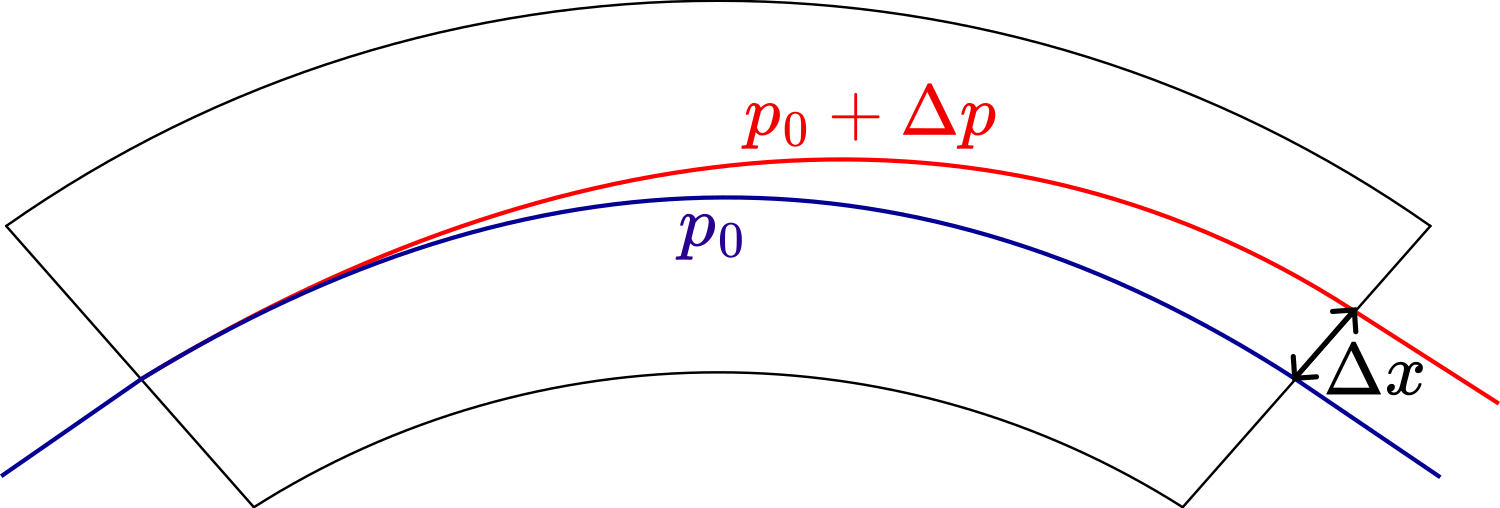
\includegraphics[width=0.6\textwidth]{images/dipole.png}
    \caption{Particles with a momentum offset will be deflected differently by dipoles. This offset
            in position can be described by the dispersion function.}
    \label{fig:coordinate_systems:dispersion}
\end{figure}

The particle is still subject to the other properties of the lattice, but with a different orbit,
described by Eq.~\eqref{fig:coordinate_systems:dispersion}.

\begin{equation}
    \begin{aligned}
    D_x(s) = \frac{\Delta x(s)}{\delta} \\
    D_y(s) = \frac{\Delta y(s)}{\delta} \\
    \end{aligned}
    \label{eq:coordinate_systems:dispersion}
\end{equation}



% ============================================
%               Beta Beating
% ============================================
\subsection{\todo{$\beta$-beating}}


% ============================================
%                  Coupling
% ============================================
\subsection{\todo{Coupling}}


% ============================================
%         Momentum Compaction Factor
% ============================================
\subsection{\todo{Momentum Compaction Factor}}


\section{Detuning Effects}


% ============================================
%                Chromaticity
% ============================================
\subsection{Chromaticity}

Chromaticity is the tune change $\Delta Q$ relative to the momentum offset $\delta$. Chromaticity
can be described by a Taylor expansion, given by

\begin{equation} 
    Q (\delta) = Q_0 + Q' \delta + \frac{1}{2!} Q'' \delta^2 + \frac{1}{3!} Q''' \delta^3 + \mathcal{O}(\delta^4).
    \label{eq:background_chromaticity}
\end{equation}

Or, more generally, rewritten as a sum to include all orders up to $n$:

\begin{equation}
    Q (\delta) = Q_0 + \sum_{i=1}^n \frac{1}{i!} Q^{(i)} \delta^i.
    \label{eq:background_chromaticity_sum}
\end{equation}


The first order of the chromaticity expansion, $Q'$, is generally simply refered to as 
\textit{chromaticity}, sometimes as \textit{linear chromaticity}.
The other terms are thus refered to as \textit{non-linear chromaticity}.

The chromaticity change induced by a single element of order $n$ and length $L$ can be derived from
the Hamiltonian of Eq.\todo{ref}, averaging over the phase variables and differentiating relative to
the actions $J_{x,y}$ and the momentum offset $\delta$:

\begin{equation}
    \Delta Q^{(n)}_{x,y} = \frac{\partial^n Q_{x,y}}{\partial^n \delta} = 
      \frac{1}{2\pi} \int_L \left< \frac{\partial^{(n+1)} H}{\partial J_{x,y}\partial^n \delta}\right> \diff s.
    \label{eq:background_chroma_order_hamiltonian}
\end{equation}


% =========
\subsubsection{Natural Chromaticity from Quadrupoles}

In a purely linear lattice, the linear chromaticity, $Q'$, is a result of the momentum dependence 
of the quadrupoles' focusing. It is in this case called the \textit{natural chromaticity} and can be
derived from the normal hamiltonian \todo{equations hamiltonian and chromaticity} and expressing the
normalized magnet strength $K$ with a dependence on $\delta$ via $P$ as $P_0(1+\delta)$:

\begin{equation}
    K_n = \frac{q}{P_0} \frac{1}{1 + \delta} (n - 1)! B_n
    \label{eq:k_dpp}
\end{equation}

The normal field of a quadrupole is then given by

\begin{equation}
    \mathcal{N}_2(x,y) = \frac{1}{2} \frac{q}{P_0} \frac{1}{1+\delta} B_2 (x^2 - y^2)
\end{equation}

By operating a variable change to the angle coordinates 
(\(x \rightarrow \sqrt{2 J_x \beta_x} \cos \phi_x\) and
\(y \rightarrow \sqrt{2 J_y \beta_y} \cos \phi_y\)), the following equation linking the $\beta$-function
and $\delta$ to the normal field is obtained:
\begin{equation}\mathcal{N}_2 (x,y) = \frac{1}{2} \frac{q}{P_0} \frac{1}{1+\delta} B_2 
        \left[
            \left(\sqrt{2 J_x \beta_x} \cos \phi_x \right)^2 
            - \left(\sqrt{2 J_y \beta_y} \cos \phi_y\right)^2
        \right].
    \label{eq:hamiltonian_quadrupole_angle}
\end{equation}

Following Eq.\ref{eq:background_chroma_order_hamiltonian}, the natural chromaticity $Q'$ induced by
quadrupoles is given by:
\begin{equation}
    \begin{aligned}
        \Delta Q'_x &= \frac{1}{2\pi} \int_L \frac{\partial^2 \left< \mathcal{N}_2 \right> }{\partial J_x \partial \delta} \diff s
        \quad;\quad
        \Delta Q'_y &= \frac{1}{2\pi} \int_L \frac{\partial^2 \left< \mathcal{N}_2 \right>}{\partial J_y \partial \delta} \diff s
        \\
        & = - \frac{1}{4 \pi} \frac{q}{P_0} B_2 L \beta_x
        & = \frac{1}{4 \pi} \frac{q}{P_0} B_2 L \beta_y
    \end{aligned}
\end{equation}


% =========
\subsubsection{Linear Chromaticity from Sextupoles}




% ============================================
%             Amplitude Detuning
% ============================================
\subsection{Amplitude Detuning}



% ============================================
%        Chromatic Amplitude Detuning
% ============================================
\subsection{Chromatic Amplitude Detuning}

\todo{make it clear I derived it}
\section{\review{Resonances}}


%----------------------------------------
%             Tune Diagram
%----------------------------------------
\subsection{\review{Tune Diagram}}

The resonances discussed in this thesis are related to the optics of the accelerator.
Such resonances create unstable motion and can lead to loosing particles.
Those perturbations arise from particles oscillating at frequencies excited by certain multipoles.

\begin{figure}[!htb]
    \centering
    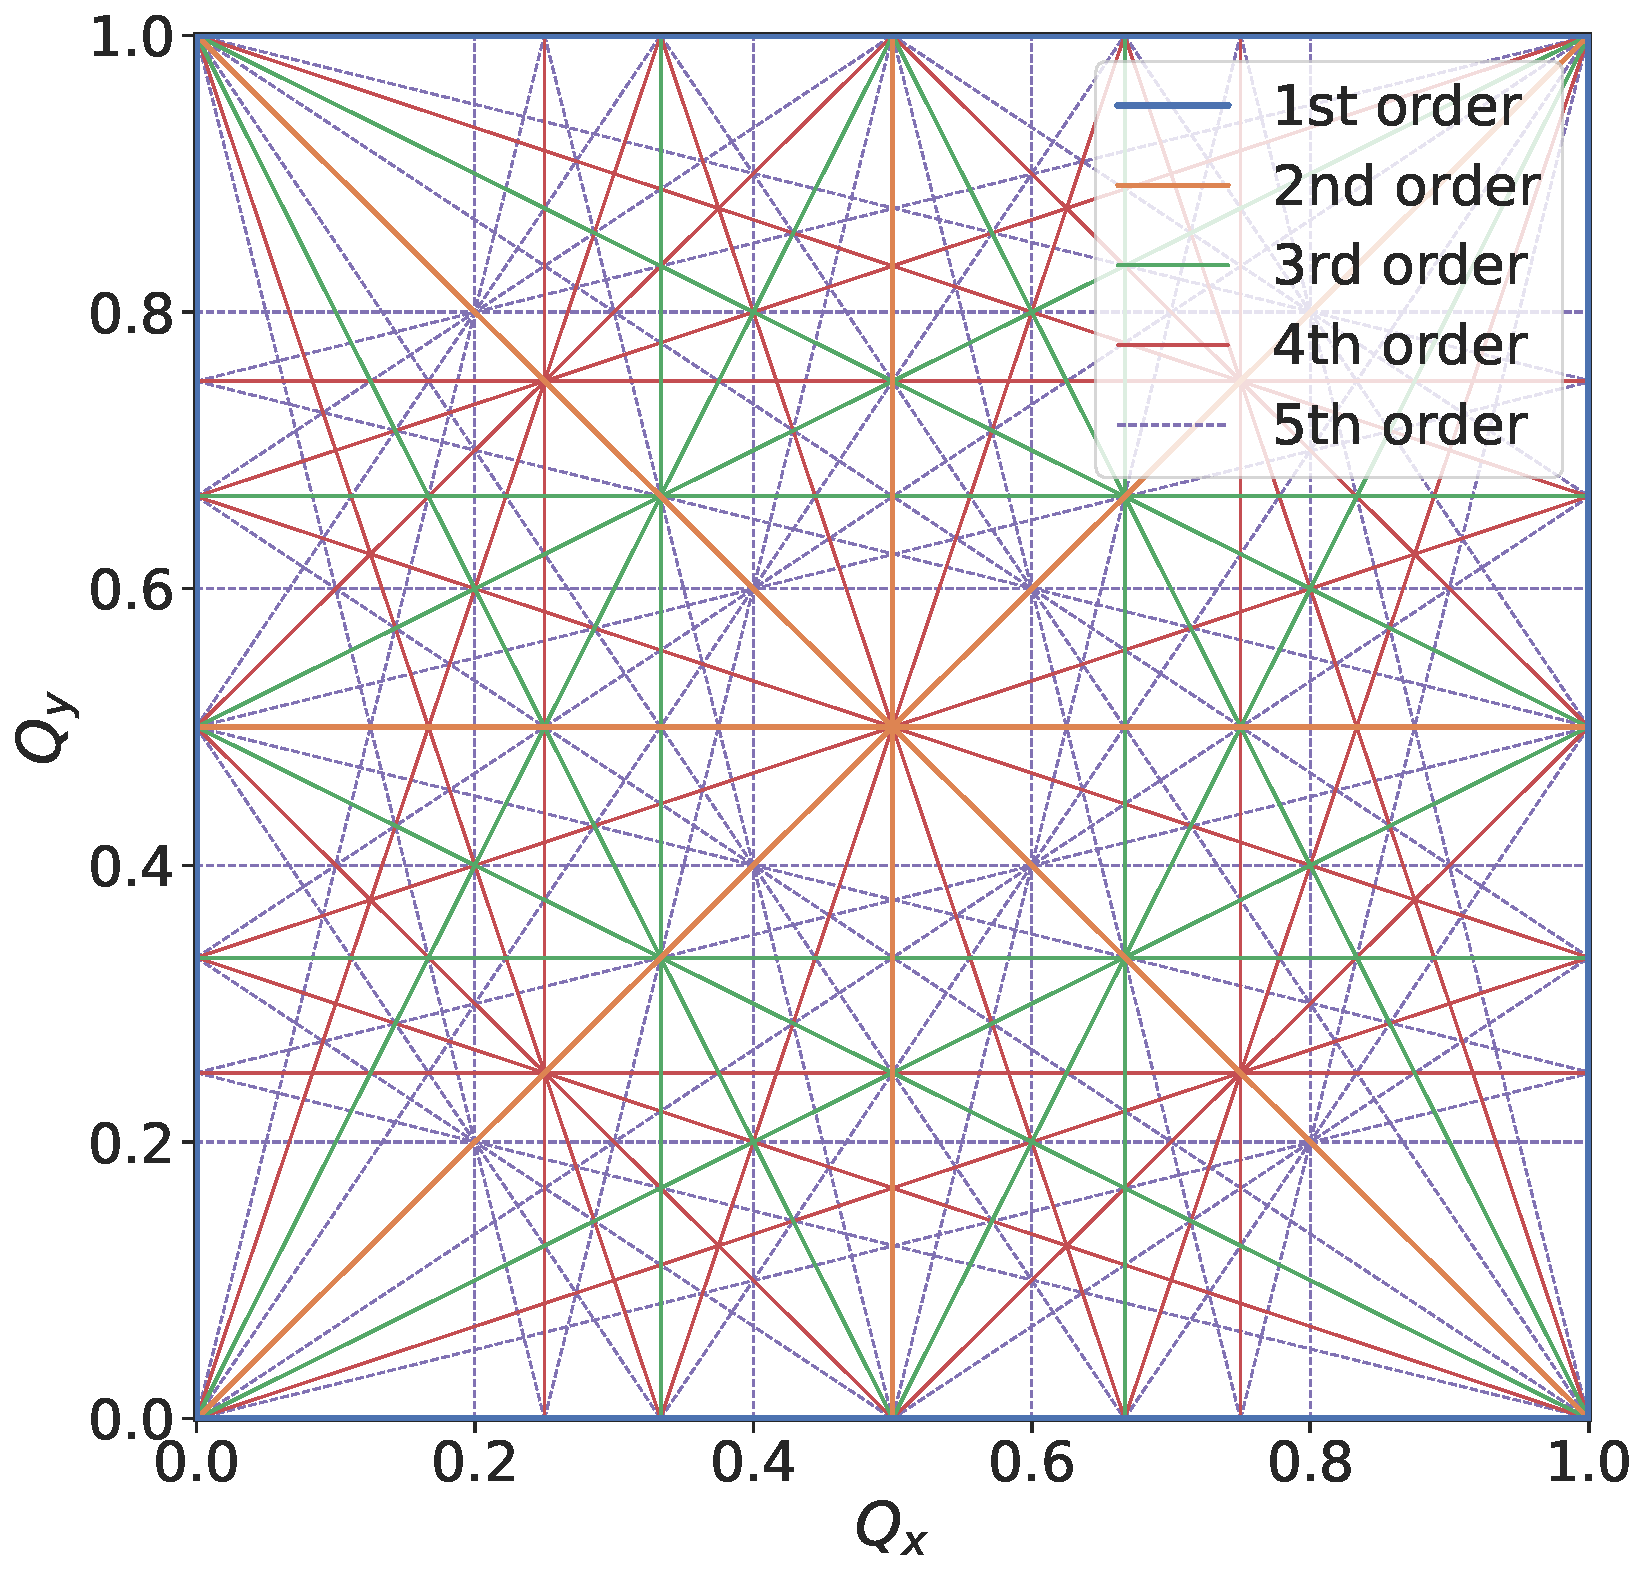
\includegraphics[width=0.82\textwidth]{images/resonance_diagram_n5.pdf}
    \caption{Tune diagram with resonances lines excited by multipoles up to decapole ($n \leq 5$).
             The working point of the machine is chosen in an area where few lines are present.}
    \label{fig:resonances:diagram_n5}
\end{figure}

\cref{fig:resonances:diagram_n5} shows a tune diagram where the fractional part of tunes $Q_x$ and
$Q_y$ can be related to resonance lines excited by multipoles up to decapoles ($n=5$).
It becomes apparent that the diagram fills quickly when considering further orders.
%, as shows \cref{fig:resonances:diagram_n7}. 
Thankfully, the higher the multipole order, the weaker the resonances are. This makes choosing a
working point possible, even if some particles are hitting resonance lines.

%\begin{figure}[H]
%    \centering
%    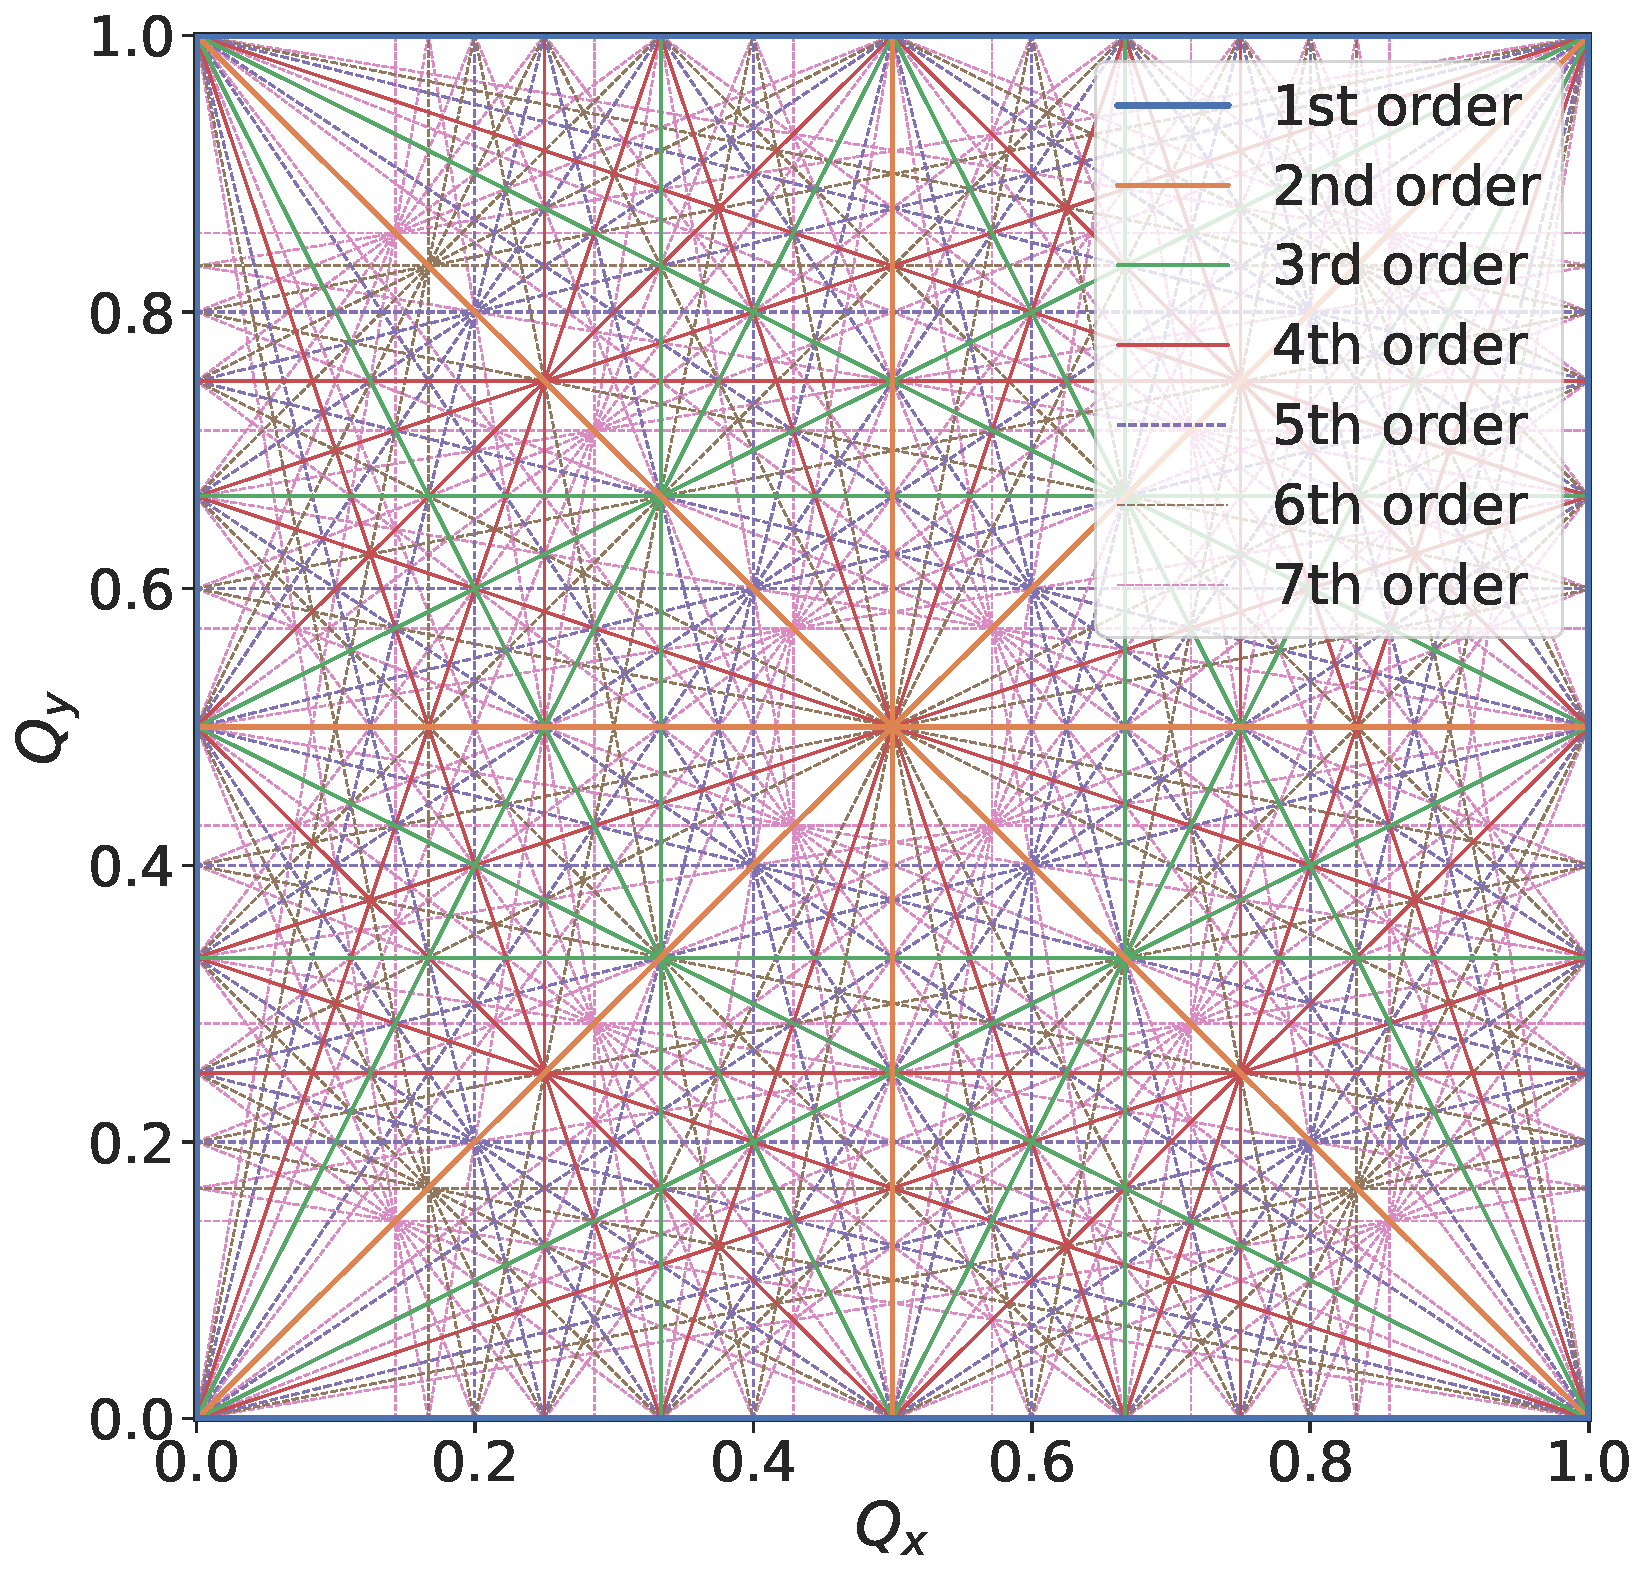
\includegraphics[width=0.82\textwidth]{images/resonance_diagram_n7.pdf}
%    \caption{Tune diagram with resonances lines excited by multipoles up to decatetrapole 
%             ($n \leq 7$). When considering higher orders, it becomes apparent that the beam will
%             inevitably hit several resonances.}
%    \label{fig:resonances:diagram_n7}
%\end{figure}


When considering the resonance driving terms $f_{jklm}$ from \cref{eq:coordinate_systems:fjklm}, it
can be noted that the term diverges for particular tune values. This leads to a disproportionate
increase in particles position in phase-space, eventually leading to loosing them.
Resonant conditions due to the tunes can thus be described by the following condition:

\begin{equation}
    (j-k)Q_x + (l-m)Q_y = p \quad,\quad j,k,l,m,p \in \mathcal{Z}.
\end{equation}
    


%----------------------------------------
%          Frequency Spectrum
%----------------------------------------
\subsection{\review{Frequency Spectrum}}

As seen in \cref{eq:coordinate_systems:linear_position_normal_form}, resonance driving terms have an
impact on the transverse position of a particle. This means that performing a FFT on such a signal
will reveal spectral lines in the frequency spectrum.
Each RDT $f_{jklm}$ can thus be observed in either one or both the frequency spectrums of the
horizontal and vertical planes, at multiples of $Q_x \pm Q_y$. \cref{eq:resonances:rdt_spectrum}
shows where those lines would appear:

\begin{equation}
    \begin{aligned}
    & H_{jklm} \;&&\text{at}\; (1 - j + k)Q_x + (m - l)Q_y \quad&&; \quad j \ne 0 \\
    & V_{jklm}   &&\text{at}\; (k - j)Q_x + (1 - l + m)Q_y      &&; \quad l \ne 0.
    \end{aligned}
    \label{eq:resonances:rdt_spectrum}
\end{equation}

The RDT $f_{3000}$ coming from sextupoles can for example be seen in the horizontal spectrum at
$(1-3+0)Q_x + (0-0)Q_y = -2Q_x$. For a value $Q_x = 0.27$, the line is seen at $0.46$. in a spectrum
bound in $[0, 0.5]$. No line can be seen in the vertical spectrum due to $l = 0$.
Detailed tables of such lines for RDTs up to order 6 can be found in \cref{appendix:rdts}.

The amplitude of each line will depend on the action $I_z$ and the amplitude of the
RDT~\cite{bartolini_normal_1997}:

\begin{equation}
    \begin{aligned}
    |H_{f_{jklm}}| &= 2 j (2 I_x)^\frac{j+k-1}{2} (2 I_y)^\frac{l+m}{2} |f_{jklm}| \\
    |V_{f_{jklm}}| &= 2 l (2 I_x)^\frac{j+k}{2} (2 I_y)^\frac{l+m-1}{2} |f_{jklm}|.
    \end{aligned}
    %\caption{\todo{FIXME}}
    \label{eq:resonances:amplitude_line}
\end{equation}


%----------------------------------------
%           RDT Calculation
%----------------------------------------
\subsection{\review{Resonance Driving Terms}}

By reworking the previous \cref{eq:resonances:amplitude_line}, it can be seen that RDTs are factors
of the line amplitude and the actions $I_x$ and $I_z$:

\begin{equation}
    \begin{aligned}
    |f_{jklm}| &= \frac{|H_{f_{jklm}}|}{2 j (2 I_x)^\frac{j+k-1}{2} (2 I_y)^\frac{l+m}{2}} \\
    |f_{jklm}| &= \frac{|V_{f_{jklm}}|}{2 l (2 I_x)^\frac{j+k}{2} (2 I_y)^\frac{l+m-1}{2}} .
    \label{eq:resonances:amplitude_rdt}
    \end{aligned}
\end{equation}

In practice, an approximation of $J = I$ is done. The RDT is then related to the fit of the line
amplitude versus the action.% as shown in \cref{fig:resonances:fit_rdt}.

%\begin{figure}[H]
%    \centering
%    \includegraphics[width=0.8\textwidth]{example-image-a}
%    \caption{.}
%    \label{fig:resonances:fit_rdt}
%\end{figure}

% ----------------------------------
% Optics Measurements and Correction
% ----------------------------------
\chapter{\review{Optics Measurements and Corrections}}
\label{chapter:optics_meas}
\section{\review{Beam Instrumentation}}


% ============================================
%          Beam Position Monitors
% ============================================
\subsection{\review{Beam Position Monitors}}

Beam Position Monitors (BPMs) are one of the most utilized and essential elements of beam 
diagnostics in particle accelerators. In the LHC, most of the BPMs are dual plane, and thus composed
of four electrodes, distributed as two per plane. The BPM system consists of over than 550 BPMs pear
beam, positioned along the ring, in the arcs and the IPs. The most common type, the
\textit{curved-button}, shown in \cref{fig:beam_instrumentation_bpm_button}, is typically placed
near quadrupoles~\cite{wendt_bpm_2020}.

\begin{figure}[!htb]
    \centering
    \begin{subfigure}[b]{0.45\textwidth}
        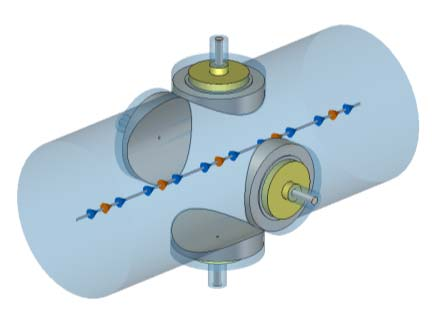
\includegraphics[width=\textwidth]{images/lhc_bpm_button.jpg}
        \caption{Button \textit{"BPM"} type BPM of the LHC~\cite{wendt_bpm_2020}.}
        \label{fig:beam_instrumentation_bpm_button}
    \end{subfigure}
    \hfill
    \begin{subfigure}[b]{0.45\textwidth}
        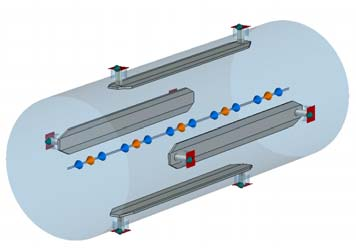
\includegraphics[width=\textwidth]{images/lhc_bpm_stripline.jpg}
        \caption{Stripline \textit{"BPMSW"} type BPM of the LHC~\cite{wendt_bpm_2020}.}
        \label{fig:beam_instrumentation_bpm_stripline}
    \end{subfigure}
\end{figure}

Other pickups such as the \textit{stripline}, shown in
\cref{fig:beam_instrumentation_bpm_stripline}, albeit more complex and expensive, offer a better
signal to noise ratio and are capable of identifying the direction of the
beam~\cite{wendt_bpm_2020}. Such features are essential for the LHC, were both beams travel through
the same aperture at the IPs.\\ 
%The BPM response is not linear with the beam position, which requires a post-processing not
%systematically implemented in accelerators beam diagnostics systems. LHC's BPMs have been simulated
%and polynomials fitted to minimize this response error~\cite{a_nosych_geometrical_2014}.


 
% ============================================
%                Collimators
% ============================================
\FloatBarrier
\subsection{\review{Collimators}}

Collimators are a crucial part of the LHC. Their purpose is to protect the machine against beam
losses and clean the outer parts of the beam~\cite{redaelli_lhc_2011}. The energy of the beams in
the LHC is high enough to not only quench the magnets, but to also damage the elements. At
injection energy, with a low intensity pilot bunch, the consequences of a loss are less severe.

%During Run 3, in 2022, a new collimator sequence was introduced, making a safe exploitation
%of the machine possible with more retracted collimators. This made measurements with higher kick
%amplitudes and larger orbit offsets, and thus momentum offsets, possible.


% ============================================
%             Beam Loss Monitors
% ============================================
\subsection{\review{Beam Loss Monitors}}

Beam Loss Monitors are detectors mounted on various elements of the accelerator, such as magnets or
collimators, to detect abnormal losses of particles. They play a crucial role in the protection of
the machine, triggering a dump when losses exceed the threshold set for their respective element. 
BLMs use ionization chambers, working on the same principle as simple Geiger counters: a tube filled
with gas, in presence of a high voltage~\cite{schmidt_machine_2014}. A picture of BLMs mounted on
the LHC is given in \cref{fig:beam_instrumentation:blm1}.

Dashboards in the control room are regularly used to monitor the losses along the ring when
performing optics measurements, as those prove to often be destructive. An example of such a
dashboard is given in \cref{fig:beam_instrumentation:blm2}.

\begin{figure}[H]
    \centering
    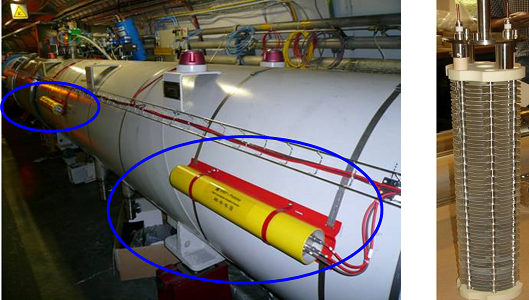
\includegraphics[width=0.6\textwidth]{images/blm.png}
    \caption{Beam Loss Monitors (BLM), in yellow, on the LHC~\cite{schmidt_machine_2014}.}
    \label{fig:beam_instrumentation:blm1}
\end{figure}

\begin{figure}[H]
    \centering
    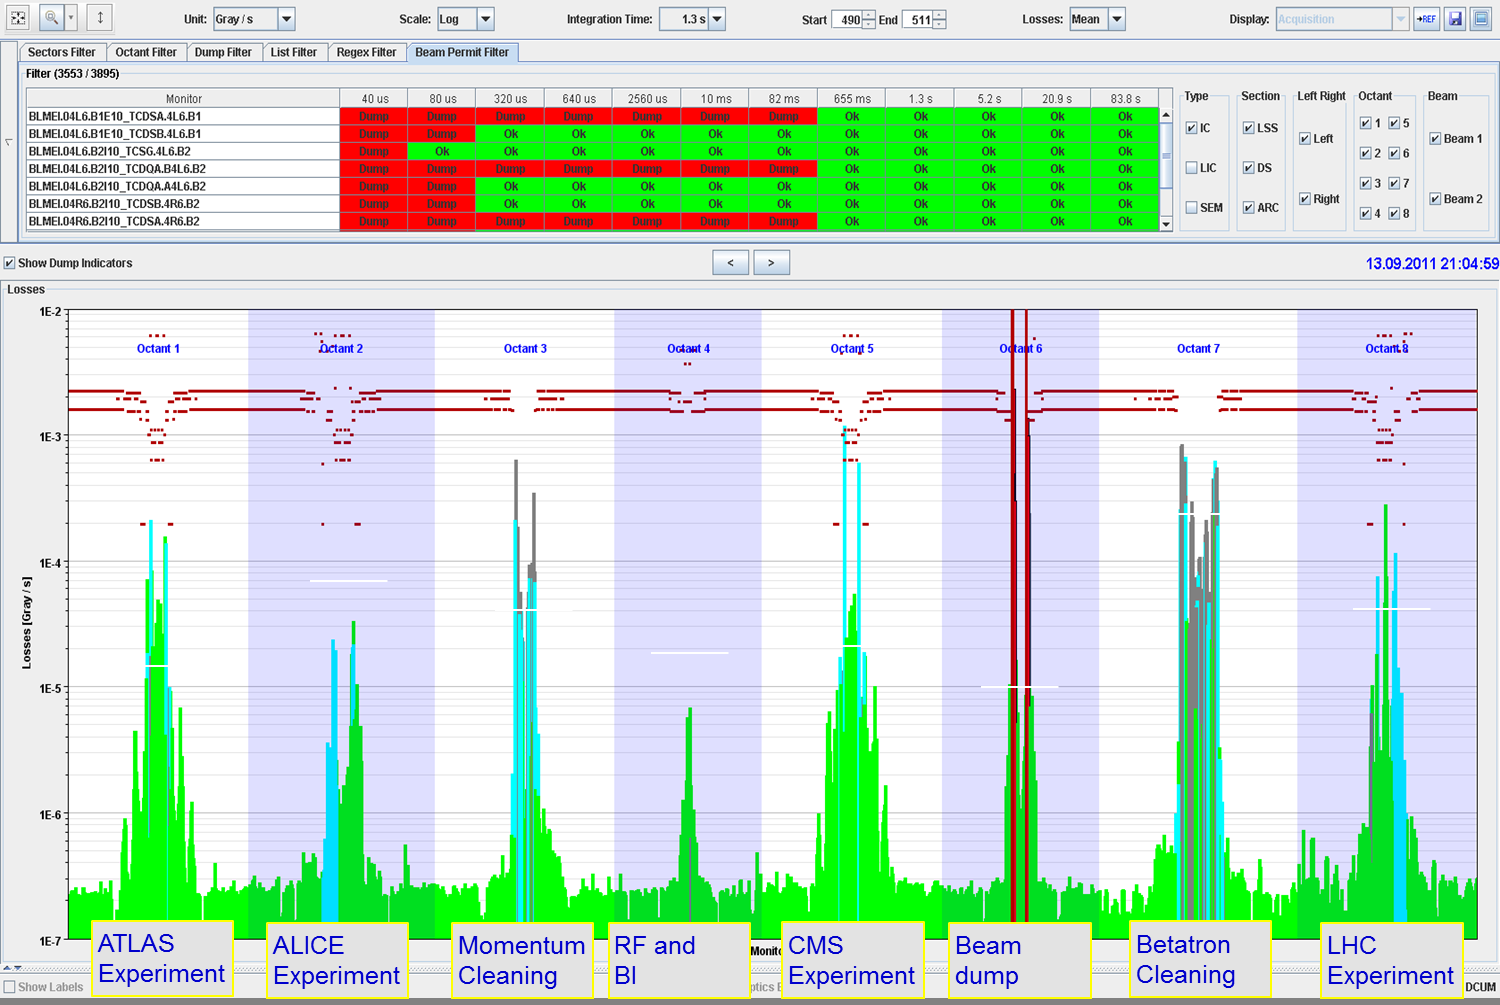
\includegraphics[width=0.6\textwidth]{images/blm2.png}
    \caption{Graphical interface used in the CERN Control Cernter (CCC) for instantaneous losses in
    the LHC~\cite{schmidt_machine_2014}. Different parts of the accelerator have varying dump
    thresholds.}
    \label{fig:beam_instrumentation:blm2}
\end{figure}


% ============================================
%                   BCT
% ============================================
\subsection{\review{Beam Current Transformer}}

The Beam Current Transformer (BCT) is a device used to measure the intensity of a particle beam by
detecting the current induced by the moving charge of the beam as it passes through the coil of the
BCT. The beam effectively acts as a primary coil and induces a current in the secondary coil of the
transformer.
The BCTs are designed to be able to measure intensities from pilots bunches of 8µA to total beams of
more than 860mA~\cite{odier_dcct_2009}. During optics measurements, beam intensity is often closely
monitored to ensure data quality, as certain observables may not be detectable at low intensities.

% ============================================
%                   BBQ
% ============================================
\subsection{\review{BBQ System}}

The Base-Band Tune (BBQ) system in the LHC is designed to measure the beam's tune via its
turn-by-turn signal. It operates by detecting and analyzing the signals of diode
peak-detectors~\cite{boccardi_first_2009,gasior_high_2005}. The system further implements processing
hardware and software, transmitting the acquired data to the control and logging systems.  The
system can operate with no explicit excitation, relying on the residual beam oscillations, or by
using tune kickers or frequency sweeps~\cite{boccardi_first_2009}.


% ============================================
%                 AC-Dipole
% ============================================
\subsection{\review{AC-Dipole}}

The AC dipole of the LHC is a crucial component for optics studies. Its primary function is to
excite the beam into large coherent oscillation, achieved by applying a sinusoidally oscillating
dipole field~\cite{miyamoto_parametrization_2008}. By ramping up and down adiabatically the
amplitude, large coherent oscillations can be produced without any decoherence or emittance growth.
\Cref{fig:ac_dipole} shows an example of a simulation made with an AC-Dipole. Exciting the beam to
large amplitudes make the study of linear optics, such as beta-beating easier, and that of non
linear optics such as resonances possible.

\begin{figure}
    \center
    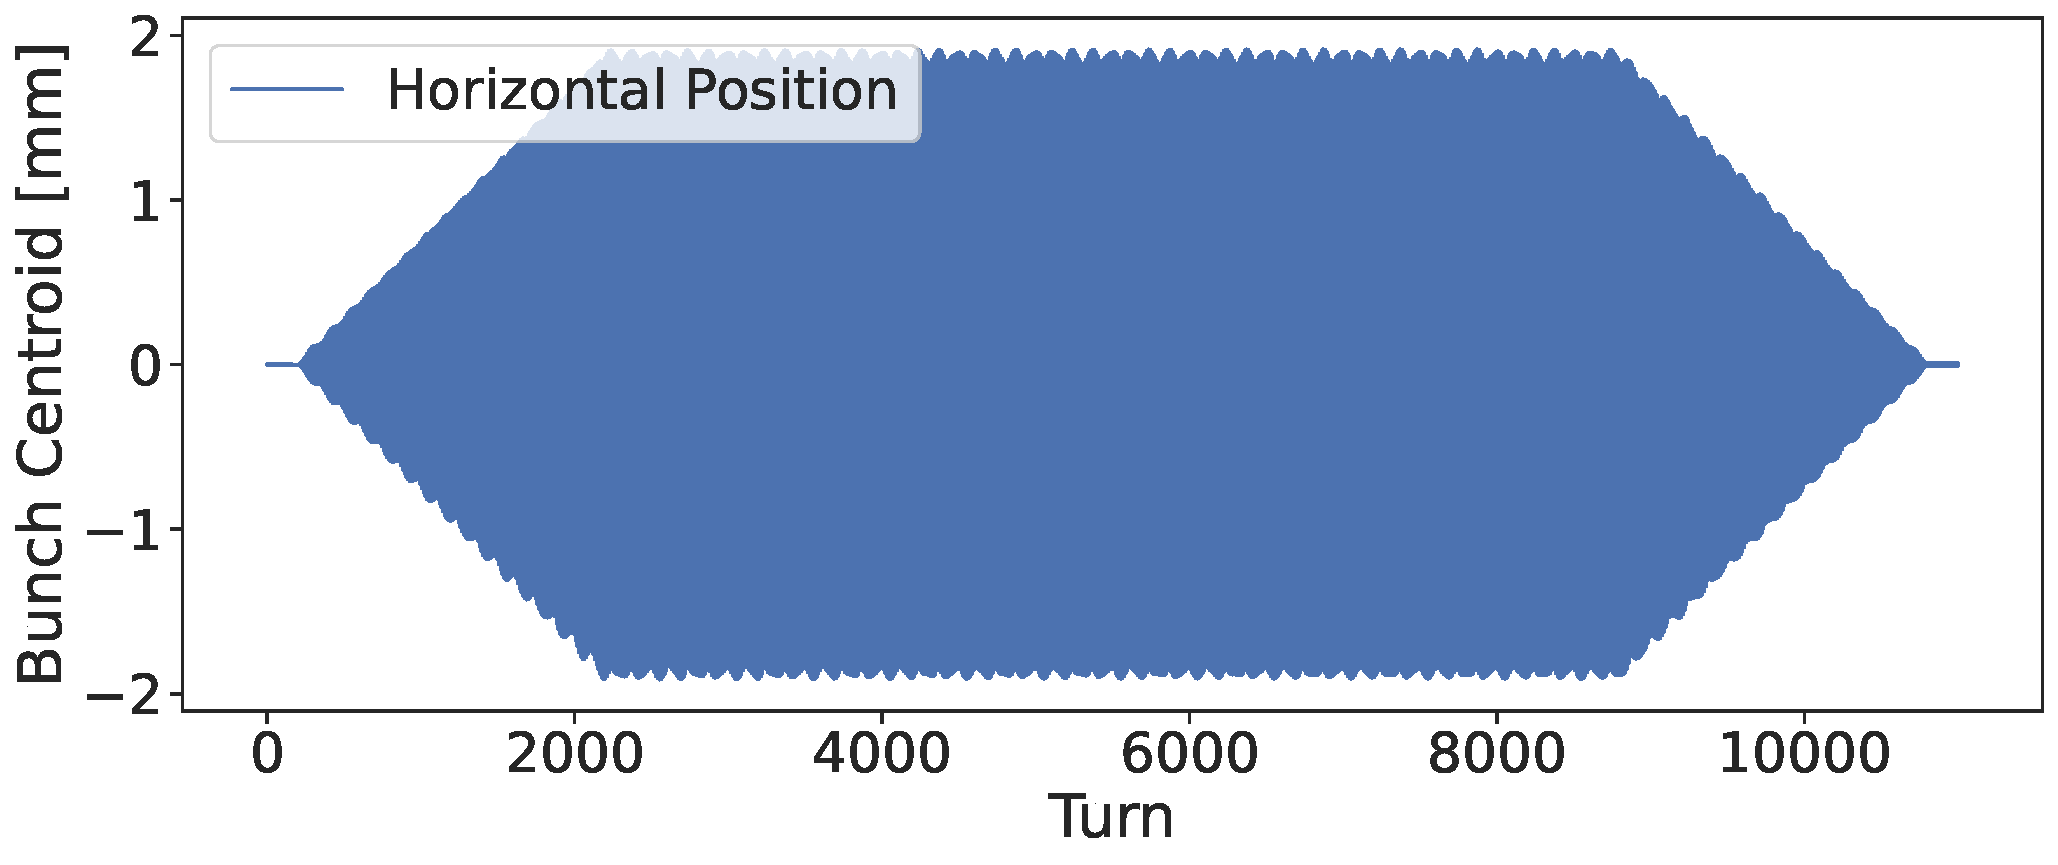
\includegraphics[width=0.85\textwidth]{./images/ac_dipole_tbt.pdf}
    \caption{Simulated turn by turn data with an AC-Dipole first ramping up then down.} 
    \label{fig:ac_dipole}
\end{figure}

The AC-Dipole is set to oscillate at a frequency $Q_d$, different from the natural tune of the
machine $Q$ and thus introduces systematic effects that needs to be compensated during the optics
analysis. The transverse position of a particle under the influence of the AC-Dipole, at turn number
$n$ and observation point $s$, is given
by~\cite{serrano_lhc_2010,tomas_normal_2002,white_direct_2013}:

\begin{equation}
z(s, n) = \frac{BL}{4\pi\rho\delta_z} \cdot \sqrt{\beta_z(s) \beta_{z,0}} \cdot \cos \left( 2 \pi Q_{d,z}n + \phi_z(s) + \phi_{z,0}\right),
\label{eq:ac_dipole}
\end{equation}

where $B$ is the amplitude of the oscillating magnetic field, $L$ the length of the AC-Dipole,
$B\rho$ the magnetic rigidity, $\delta$ the difference between $Q_d$ and $Q$, $\beta$ and $\beta_0$
the beta function at the observed point and the AC-Dipole, $\phi$ and $\phi_0$ the phase advance at
the observed point and of the AC-Dipole.
% ===============================
%        Optics Measurements
% ===============================

\subsection{Turn by Turn}





% ================================================= 
%                   Chromaticity
\subsection{Chromaticity}

% --- Procedure ---
\subsubsection{Procedure}

Chromaticity measurements are typically performed by varying the RF frequency to induce a change of momentum offset $\delta$, while measuring the tune.
The momentum offset $\delta$ being related to the RF frequency and the momentum compaction factor $\alpha_c$:

\begin{equation}
    \delta = - \frac{1}{\alpha_c} \cdot \frac{\Delta f_{RF}}{f_{RF,nominal}}
    \label{eq:dpp_rf}
\end{equation}

Frequency steps of 20Hz every 30 secondes are typically taken to compromise between number of data points, precision of the tune estimate, and duration of the measurement.
Once beam losses, registered by the Beam Loss Monitors (BLM), are deemed too high, the frequency is reverted back to its nominal value in larger steps. The same procedure is then re-applied in the negative. Figure \ref{fig:measurements:rf_scan} shows a typical RF scan performed to measure chromaticity in the LHC.

\begin{figure}[H]
    \centering
    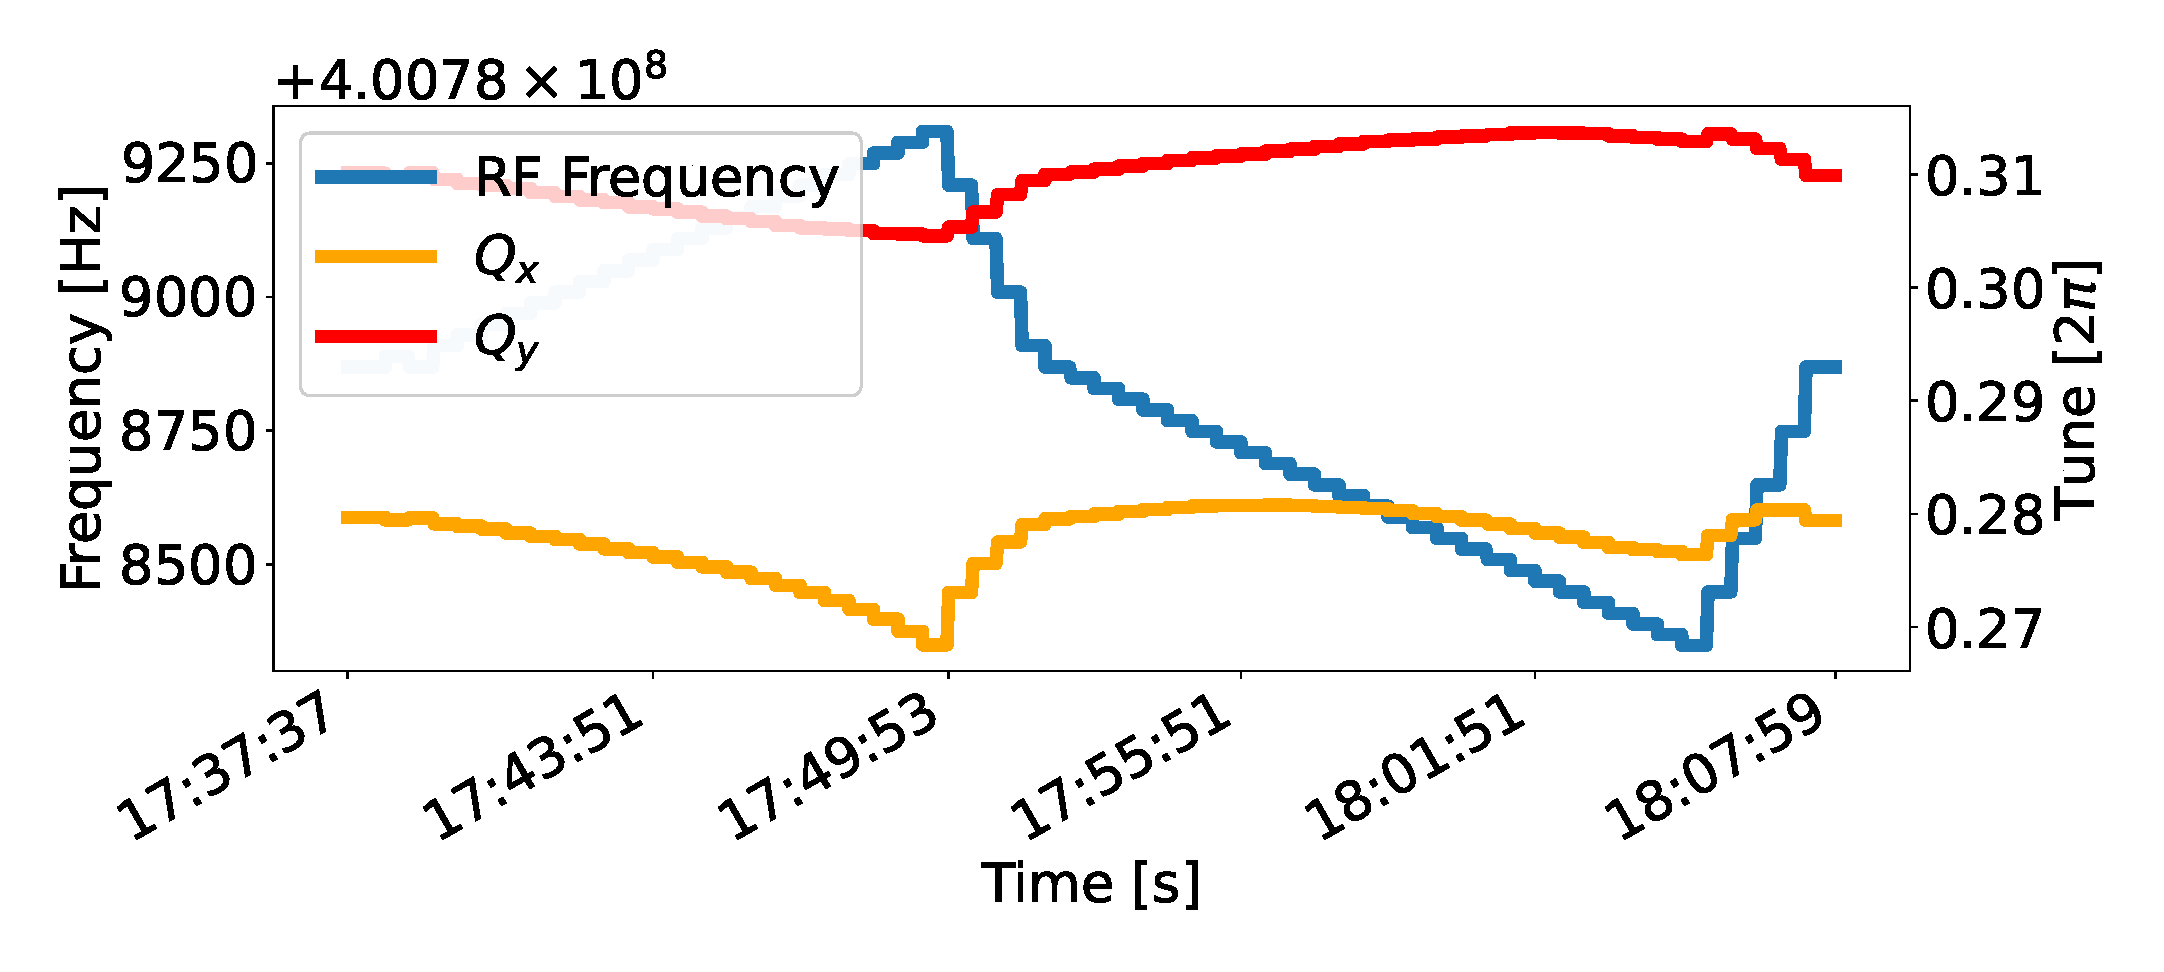
\includegraphics[width=1\textwidth]{images/rf_scan.pdf}
    \caption{Observation of the tune dependence on momentum offset, created by a shift of RF frequency}
    \label{fig:measurements:rf_scan}
\end{figure}




% --- Analysis and Fit ---
\subsubsection{Analysis}

\section{Correction Principles}


% ===============================
%        Response Matrix
% ===============================
\subsection{\review{Response Matrix}}

A response matrix is a linear equation system that describes the change of an observable for a set of individual multipole strengths. By taking the pseudo-inverse of this matrix and multiplying it to the measured observables, a set of corrector strengths if obtained that can replicate the measured value. Taking the opposite sign then gives a correction.
This technique is routinely used to correct, amongst others, \beta-beating as well as Resonance Driving Terms. In situations where measurements are taken at each BPM for a particular observable, the corresponding response matrix ends up containing over 500 values per corrector, for a single beam.

Individual MAD-X simulations are run with a single multipole powered at a time. The resulting parameter values (e.g. \beta-beating) are then compared to those obtained from a simulation without any powering, allowing to determine the specific impact of each multipole.

A response matrix is thus created following eq.\ref{eq:resp_matrix}, for a matrix of observables $O$, a reference matrix of observables without any corrector $O_R$ and a fixed multipole strength $k$. Given measured data $M$, the set of correctors needed to compensate the values can be obtained by taking the pseudo-inverse of the matrix in eq.\ref{eq:resp_matrix_inverted}.

\begin{equation}
  R = \left(O - O_R \right) \cdot \frac{1}{k}
  \label{eq:resp_matrix}
\end{equation}

\begin{equation}
  \begin{bmatrix}
    k_1 \\
    \vdots \\
    k_n \\
  \end{bmatrix}
  = -(R^{+} \cdot M)
  \label{eq:resp_matrix_inverted}
\end{equation}
 
Response matrices are very versatile and can combine several observables to be corrected by the same multipoles. One example, detailed later in this thesis, is the third order chromaticity and the resonance driving term $f_{1004}$, both contributed to by decapoles.

\subsubsection{Example}

In this example, simulations are run with MAD-X PTC to correct the third chromaticity in the LHC.
$Q'''$ is taken from \verb|ptc_normal| for each beam and axis, with \verb|MCDs|, decapole correctors, powered with a fixed strength one at a time. A scaling factor is applied to get the change of chromaticity for one unit of $K_5$.
8 correctors are used, which strengths are denoted $k_1$ through $k_8$.
Transposes are only used to make the equations easier to display.\\
The values in Tab.\ref{table:resp_matrix_example} are corrected via 
Eq.~\eqref{eq:resp_matrix_inverse_example} after having built the response matrix in Eq.~\eqref{eq:resp_matrix_example}.

\begin{table}[H]
  \center
  \begin{tabular}{c c c}
      Observable & Value \\
      \hline
      $Q'''_x$ & -666111 \\
      $Q'''_y$ &  121557 \\
  \end{tabular}
  \caption{Example chromaticity values to correct via a response matrix}
  \label{table:resp_matrix_example}
\end{table}

% ====
\vspace{0.4cm}
\begin{equation}
  R
  %
  =
  %
  \left(
    %{\text{Individual} \atop \text{simulations}}
    {\genfrac{}{}{0pt}{0}{\text{Individual}}{\text{simulations}}}
    \left\{
      \begin{bNiceMatrix}
       -155899  &  122004 \\  
       -254584  &  138368 \\
       -122715  &  106709 \\
       -218597  &  110686 \\
       -134140  &  106463 \\
       -245791  &  118951 \\
       -147035  &  116544 \\
       -219537  &  112317 \\
        \CodeAfter
        \OverBrace{1-1}{1-1}{Q'''_x}[yshift=2mm]
        \OverBrace{1-2}{1-2}{Q'''_y}[yshift=2mm]
      \end{bNiceMatrix}^T
    \right.
    -
    \left.
    \begin{bNiceMatrix}
       5135 \\
       8470 \\
      \CodeAfter
      \OverBrace{1-1}{1-1}{\scriptstyle \text{Reference}}[yshift=2mm]
    \end{bNiceMatrix}
    \right\}
    {\genfrac{}{}{0pt}{0}{Q'''_x}{Q'''_y}}
  \right)
  %
  \cdot
  %
  \underbrace{\frac{1}{-1000}}_{\text{Corrector strength}}
  \label{eq:resp_matrix_example}
\end{equation}
\vspace{0.5cm}


% Inverting the response matrix
\begin{equation}
    \begin{matrix}
      k_1 \\
      k_2 \\
      k_3 \\
      k_4 \\
      k_5 \\
      k_6 \\
      k_7 \\
      k_8 \\
    \end{matrix}
  \left\{
  \begin{pmatrix}
     -1235 \\
      1032   \\  
     -1394  \\ 
      1449   \\ 
     -1043  \\ 
      1864   \\ 
     -1187  \\ 
      1369   \\ 
  \end{pmatrix}
  \right.
  %
  =
  %
  -R^{+} 
  %
  \cdot
  %
  \left.
  \begin{pNiceMatrix}
      -666111 \\
      121557 \\
  \end{pNiceMatrix}
  \right\}
  %{\text{Measured} \atop \text{values}}
  {\genfrac{}{}{0pt}{0}{\text{Measured}}{\text{values}}}
  \label{eq:resp_matrix_inverse_example}
\end{equation}





% ===============================
%    Chromaticity Global Trim
% ===============================
\subsection{\review{Global Trims for Chromaticity}}

% ~~~~~~~~~~~~~~~~~~~~~~~~~~~~~
% The script for the linearity can be found in
% /afs/cern.ch/work/m/mlegarr2/public/jupyter/chromaticity/simulations/linearity_dq3_mcd

As per the placement of the MCO and MCD spool piece correctors in the LHC 
layout~\cite{maclean_commissioning_2016-1}, $\beta$-functions at their location are slightly
different from arc to arc. This slight imbalance leads theoretically to the possibility of
correcting the horizontal and vertical axes of the second and third order chromaticity
independently, via a response matrix approach. In practice, the required strength to do so would
exceed those of the design of the correctors.

Another way to correct the chromaticity is via a global uniform trim, where every available
corrector is powered to the same strength.  Simulations are run with \verb|ptc_normal| via MADX-PTC
to obtain the response in chromaticity for a given strength. Chromaticity being linear with
multipole strength, an affine function can be determined for each axis. Figure
\ref{fig:corrections-dq3_versus_k5} shows a simulation with several MCD strengths, highlighting this
linear relation between $Q'''$ and $K_5$, while
Equation~\eqref{eq:corrections:chromaticity_affine_function_ptc} shows an example of such functions computed
at injection energy for the 2022 optics.

\begin{figure}[H]
  \centering
  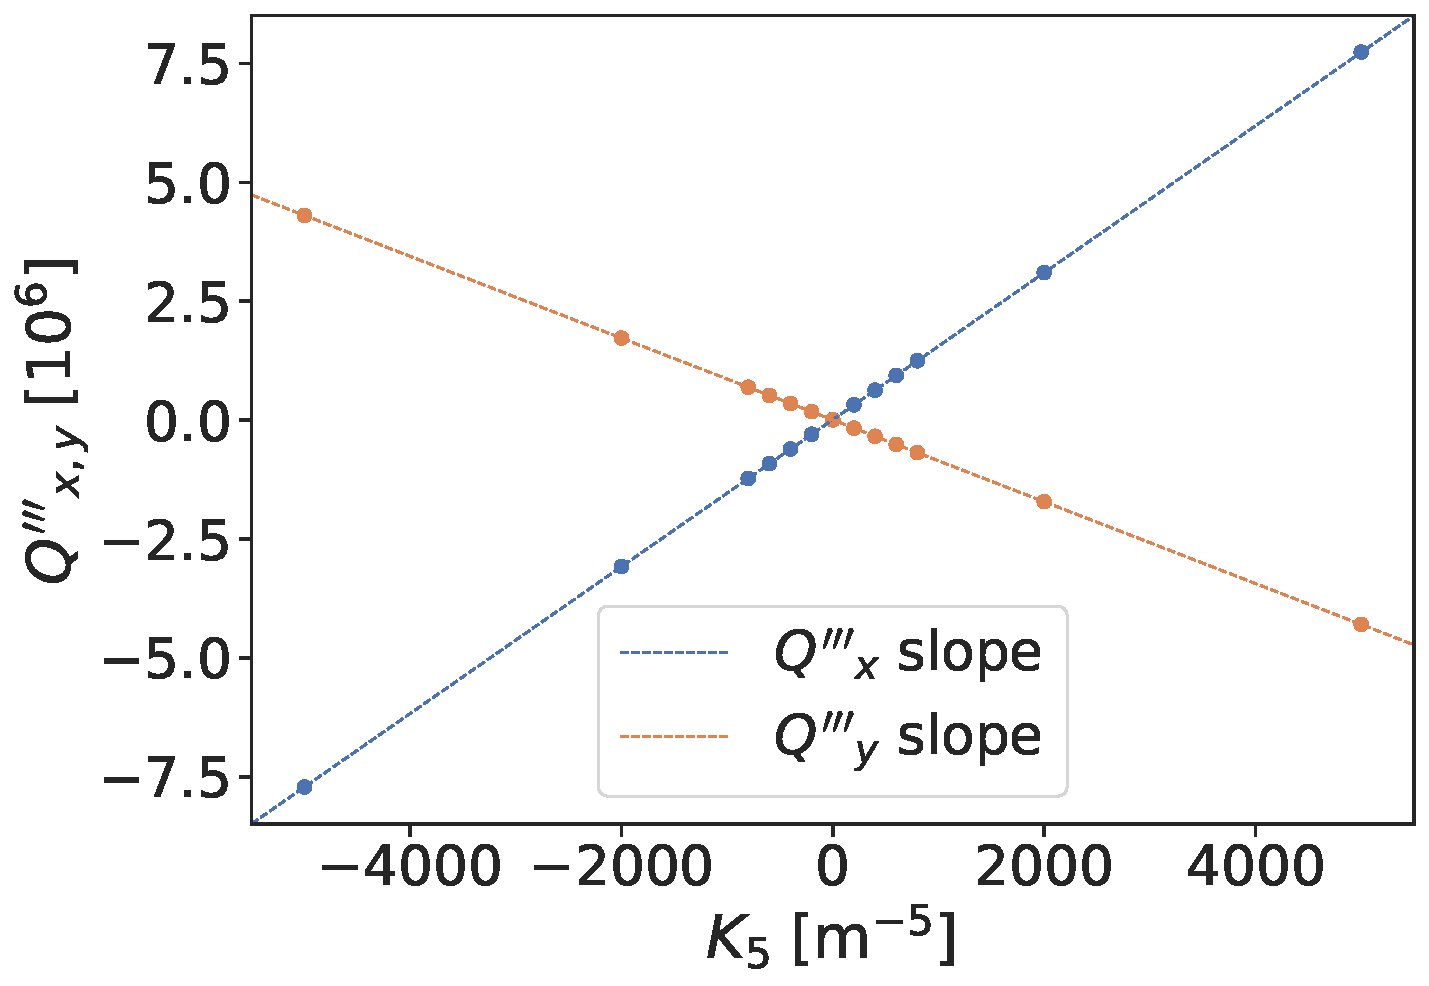
\includegraphics[width=0.6\textwidth]{images/dq3_k5.pdf}
  \caption{Linear relation between the third order chromaticity and decapole corrector strengths,
           simulated with MADX-PTC.}
  \label{fig:corrections-dq3_versus_k5}
\end{figure}

\begin{equation}
  \begin{aligned}
    &Q'''_x = 1533 \cdot \Delta K_5 + 6680 \\
    &Q'''_y = -860 \cdot \Delta K_5 + 5647
  \end{aligned}
  \label{eq:corrections:chromaticity_affine_function_ptc}
\end{equation}

Only the linear part is relevant, as the offset is generated by other multipoles and field errors.
It is thus constant for a configuration where only the relevant spool pieces are used.

Corrections involve minimizing both axes, typically where $Q'''_x$ meets $Q'''_y$:

\begin{equation}
  \Delta K_5 = -\frac{(Q'''_x - Q'''_y)}{\text{slope}_{Q'''_x} - \text{slope}_{Q'''_y}}
  \label{eq:corrections:chromaticity_global_correction}
\end{equation}

% ----------------------------------
%       Skew Octupolar Fields
% ----------------------------------
\chapter{\review{Skew Octupolar Fields}}
\label{chapter:skew_octupole_fields}
%=============================
%        Introduction
%=============================
\section{\review{Introduction}}

The skew octupolar fields in the LHC have previously been identified as significant contributors to 
limits in forced dynamic aperture, being the dynamic aperture when kicking the beam with the
AC-Dipole~\cite{carlier_nonlinear_2020}. Skew octupolar correctors are positioned around the
ATLAS and CMS detectors, in Interaction Regions 1 and 5. Those correctors are \textit{common
aperture} magnets ; both beams are affected by the created magnetic fields. Unfortunately, one of
these four correctors, located to the left of ATLAS, is not functioning. As a result, although
corrections can be calculated, they will not effectively minimize the skew octupolar RDTs of
interest, $f_{1012,y}$ and $f_{1210,x}$. 
The associated resonances and frequency lines of these RDTs are shown in
\cref{tab:skew_octupolar:resonances_rdts}.

\begin{table}[!htb]
    \centering
    \begin{tabular}{lccc}
      \toprule
      RDT         & Resonance                &  H-line                    & V-line         \\
      \midrule
      $f_{1012}$  & $\phantom{-}1Q_x - 1Q_y$ &  $\phantom{2Q_x-\ \,}1Q_y$ & $-1Q_x + 2Q_y$ \\
      $f_{1210}$  & $-1Q_x + 1Q_y$           &  $2Q_x - 1Q_y$             & $\phantom{-}1Q_x\phantom{+2Q_y\ \,}$    \\
      \bottomrule
    \end{tabular}
    \caption{Skew octupolar RDTs of interest, their associated resonances and the frequency spectrum
    lines they contribute to.}
    \label{tab:skew_octupolar:resonances_rdts}
\end{table}

First corrections of skew octupolar RDTs were performed in 2018 at top
energy~\cite{carlier_nonlinear_2020}. A different approach for the same corrections is presented in
this chapter.
Measurements were also performed at injection energy with the prospect of corrections. However, it
was observed that Landau octupoles were strongly contributing to the RDTs of interest.


%=============================
%         Top Energy
%=============================
\section{\review{Corrections at Top Energy}}

The very first skew octupolar RDT corrections in the LHC were made in 2018 during
Run~2~\cite{carlier_nonlinear_2020}. These corrections were computed by matching the RDT level of
the measurements in simulation and then inverting the strengths. This is possible and remains viable
as only three correctors are used and values can be manually adjusted.
In this section, a different approach is taken, based on response matrices. This type of correction
is explained in details in \cref{correction_principle:response_matrix}. The real and imaginary 
responses of the RDTs for each corrector at an arbitrary strength are simulated through tracking.
These responses are collected into a matrix, allowing the determination of the required strengths to
match the RDT level observed in the measurements. Inverting these values result in a correction.


%-----------------------------
%     Correctors Response
%-----------------------------
\subsection{\review{Correctors}}

To create a response matrix, simulations were conducted with the tunes and AC-Dipole deltas set to
those used for measurements. The natural tunes are $Q_x = 0.285$ and $Q_y = 0.292$ while the driven
tunes are $\Delta Q_x = -0.008$ and $\Delta Q_y = 0.01$. Each corrector is then powered
individually for each tracking simulation. For this type of simulation, field errors are not
necessary, as only the RDT shift caused by the corrector relative to the baseline is needed.
\Cref{fig:skew_octupolar:response_correctors} shows the real part of the resulting RDTs from these
simulations for Beam 1. Beam 2 shows a similar level of response for these correctors.

\begin{figure}[!htb]
    \centering
    \begin{subfigure}{0.8\textwidth}
        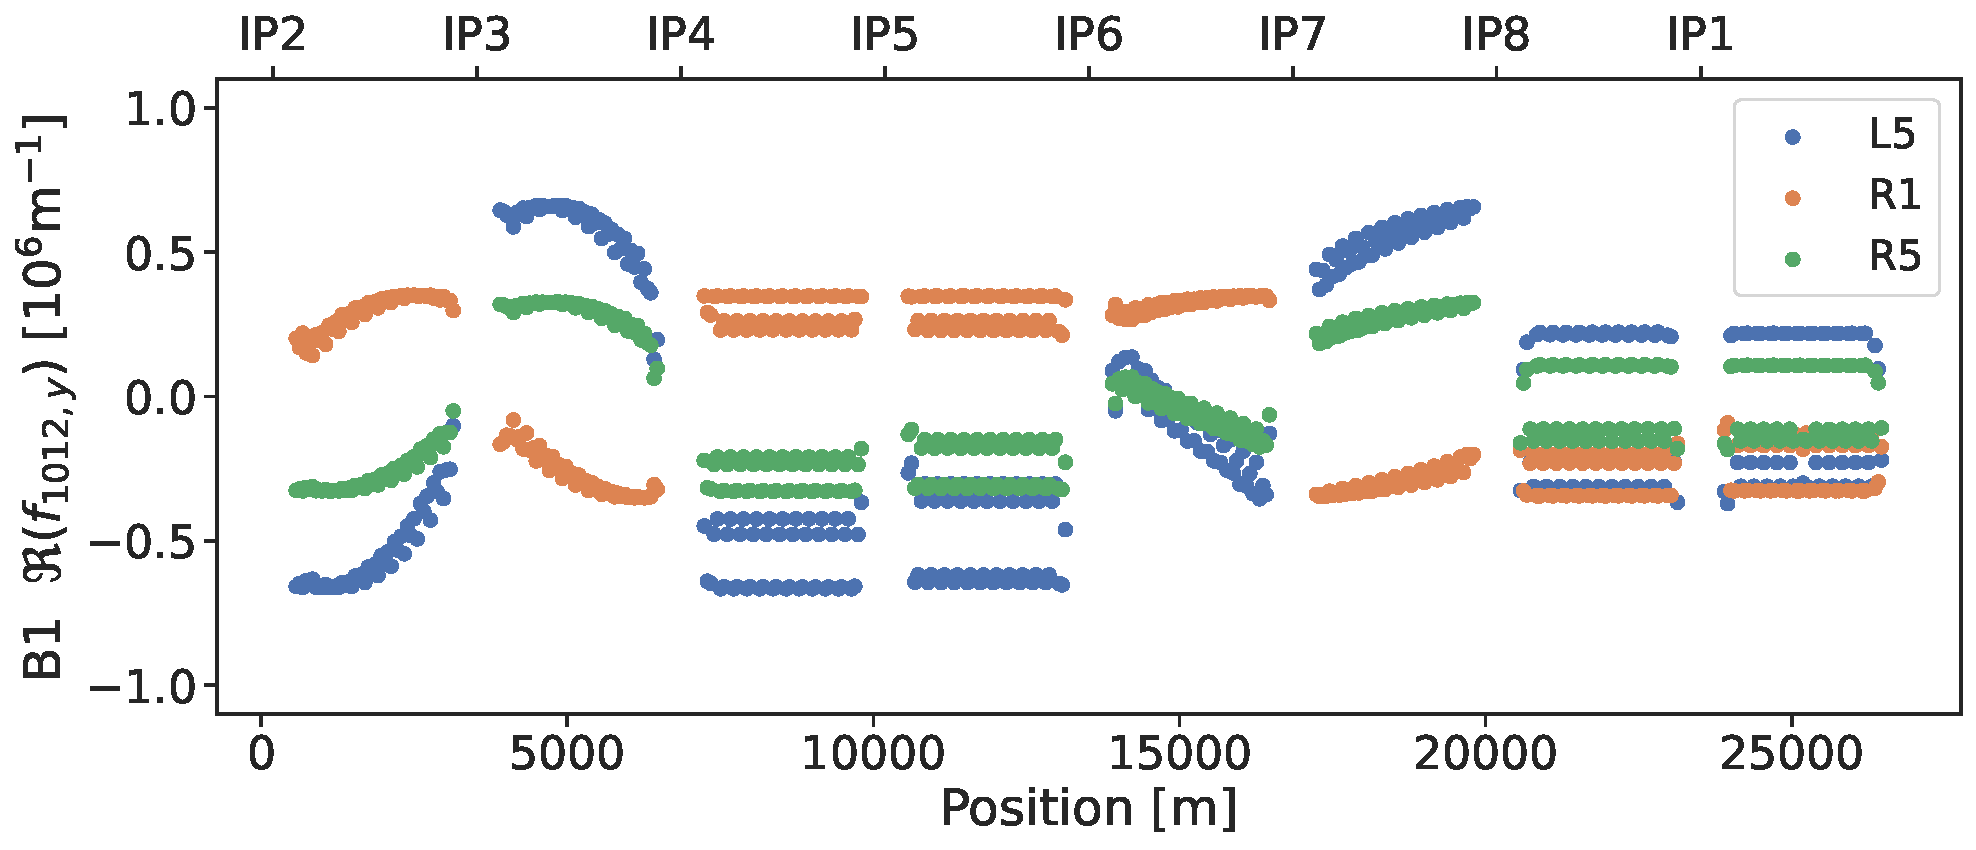
\includegraphics[width=\textwidth]{./images/f1012_b1_correctors.pdf}
        \caption{$f_{1012,y}$}
    \end{subfigure}
    \par\bigskip 
    \begin{subfigure}{0.8\textwidth}
        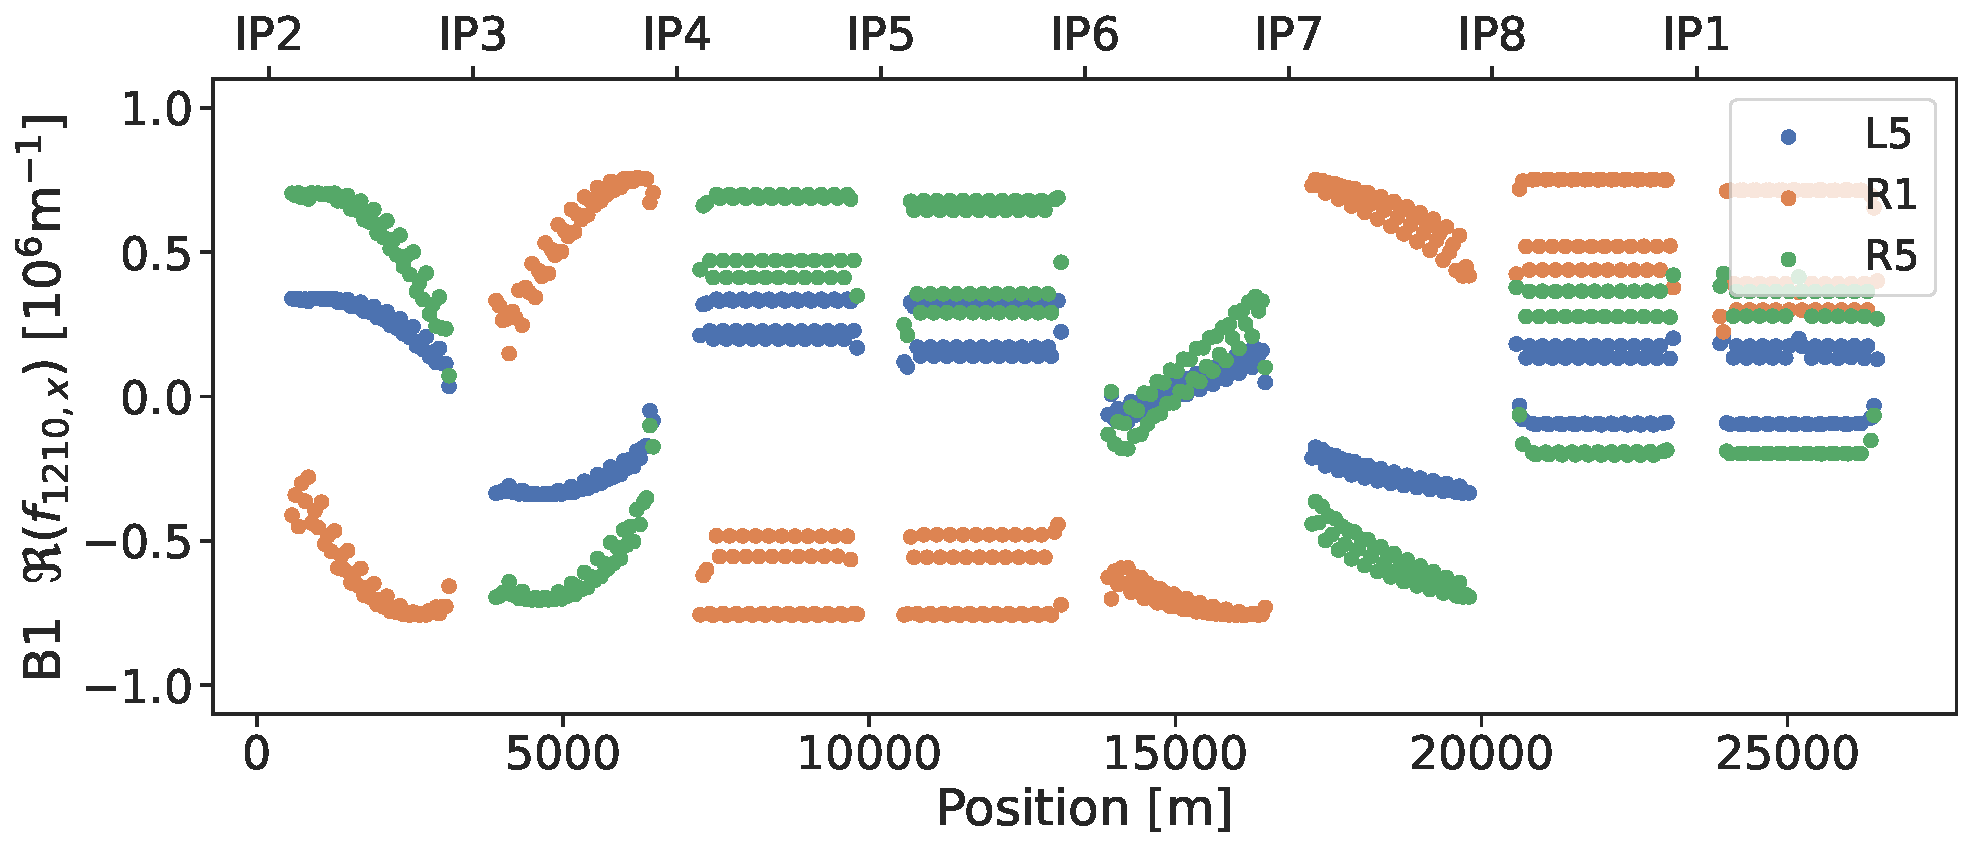
\includegraphics[width=\textwidth]{./images/f1210_b1_correctors.pdf}
        \caption{$f_{1210,x}$}
    \end{subfigure}
    \caption{Simulation of the RDT response of the skew octupolar correctors at top energy for Beam
    1. Each corrector is powered at $J_4 = 1 [\text{m}^{-4}]$.}
    \label{fig:skew_octupolar:response_correctors}
\end{figure}

It can already be seen that the L5 and R5 correctors show a similar trend along the ring, with L5
showing a stronger response for the same strength, while the R1 corrector follows the opposite
trend. A polar plot at a given BPM can illustrate that trend, and be used to get an intuition of the
effect of the correctors to manually compute corrections.
\Cref{fig:skew_octupolar:response_correctors_polar} shows the orthogonality of the correctors for
both beams and RDTs. L5 being stronger than R5 while having the same angle indicates that only one
of them is needed for corrections. 

\begin{figure}[!htb]
    \centering
    \begin{subfigure}{0.8\textwidth}
        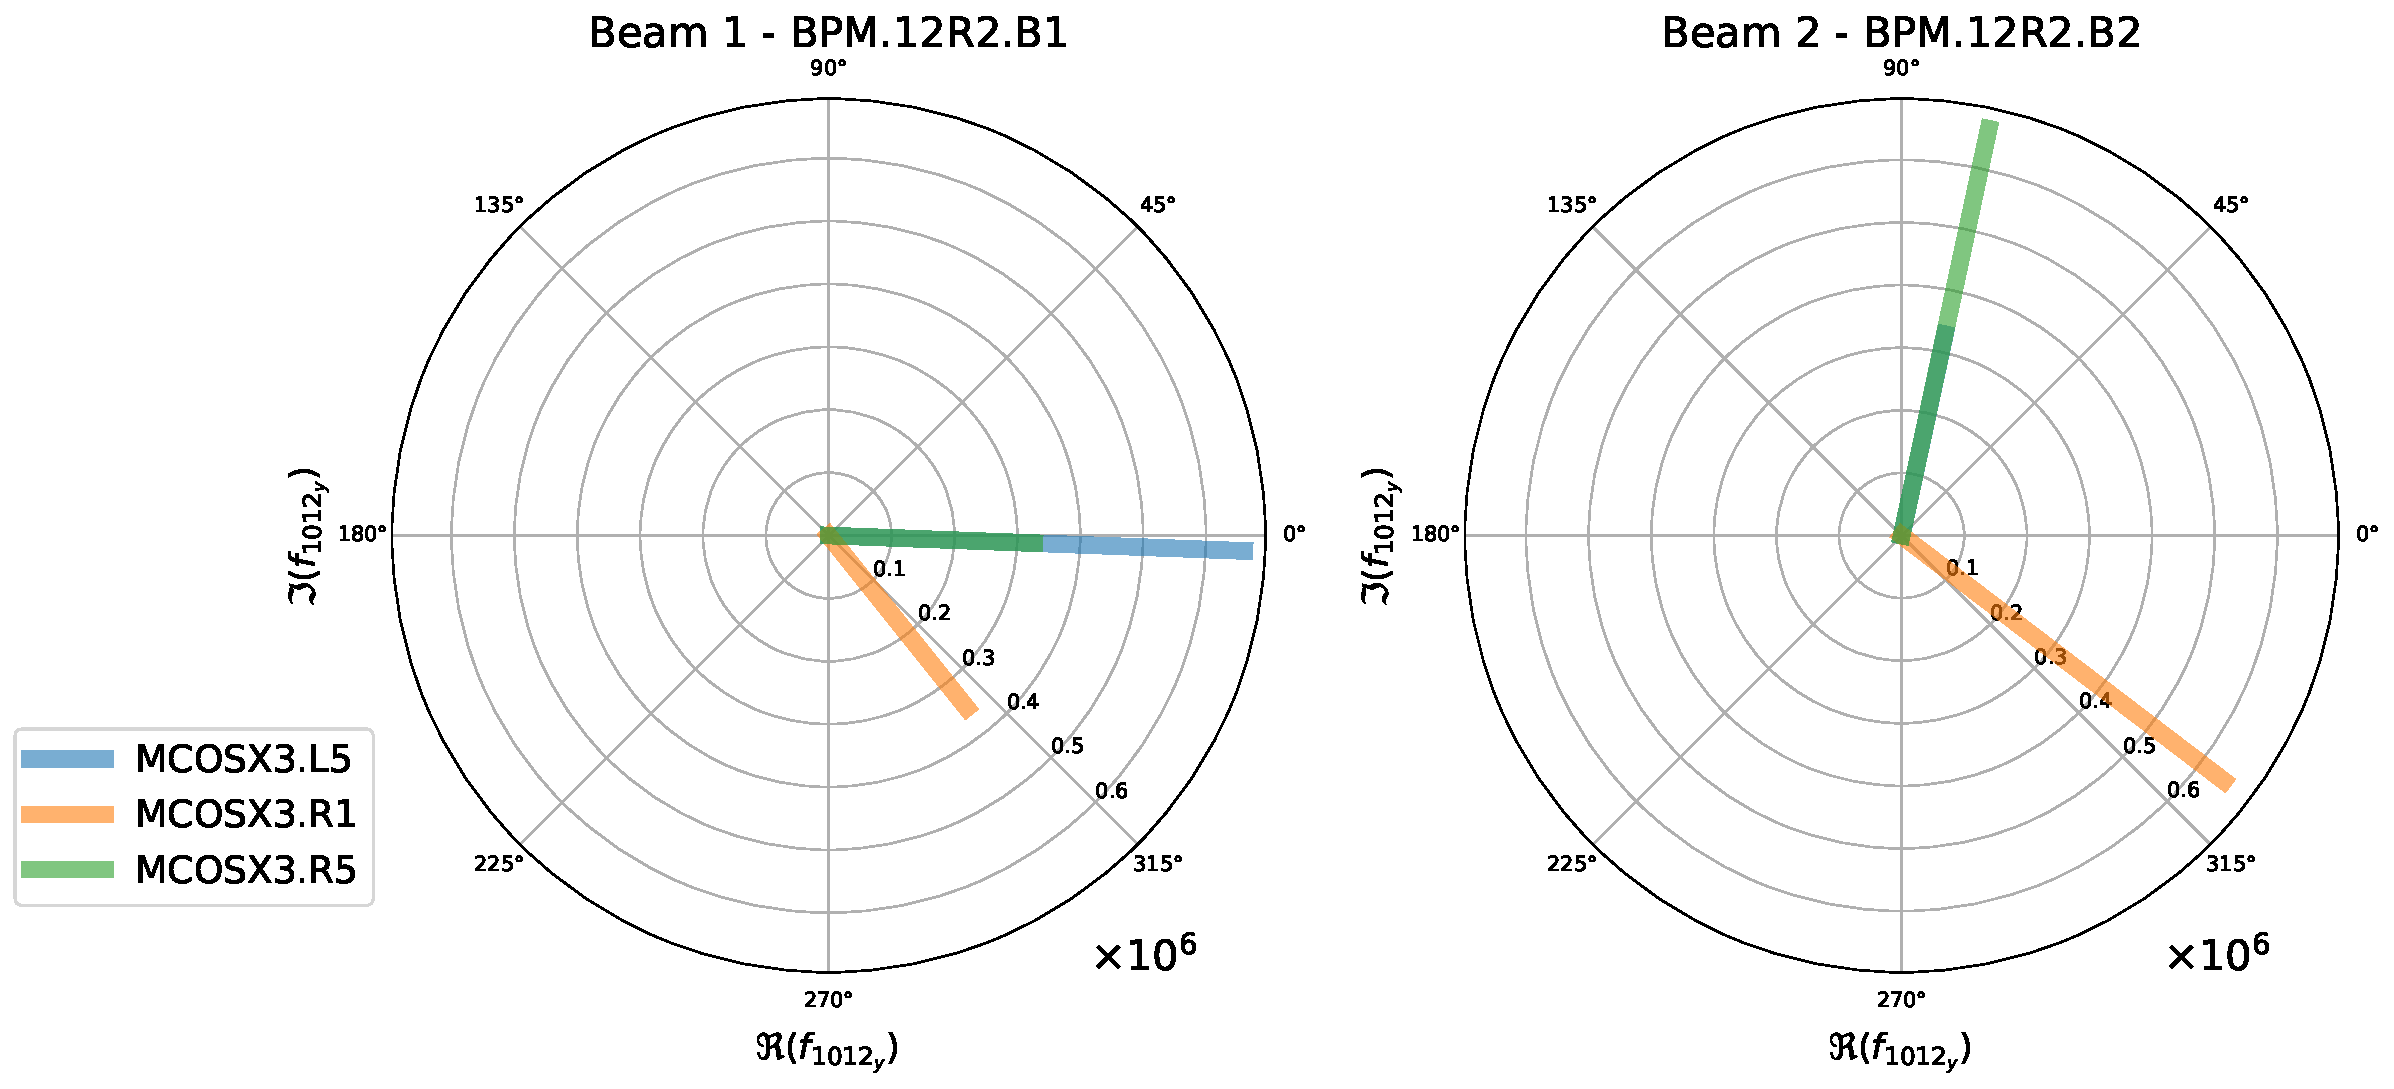
\includegraphics[width=\textwidth]{./images/orthogonal_a4_inj_f1012_y.pdf}
        \caption{$f_{1012,y}$}
    \end{subfigure}
    \par\bigskip 
    \begin{subfigure}{0.8\textwidth}
        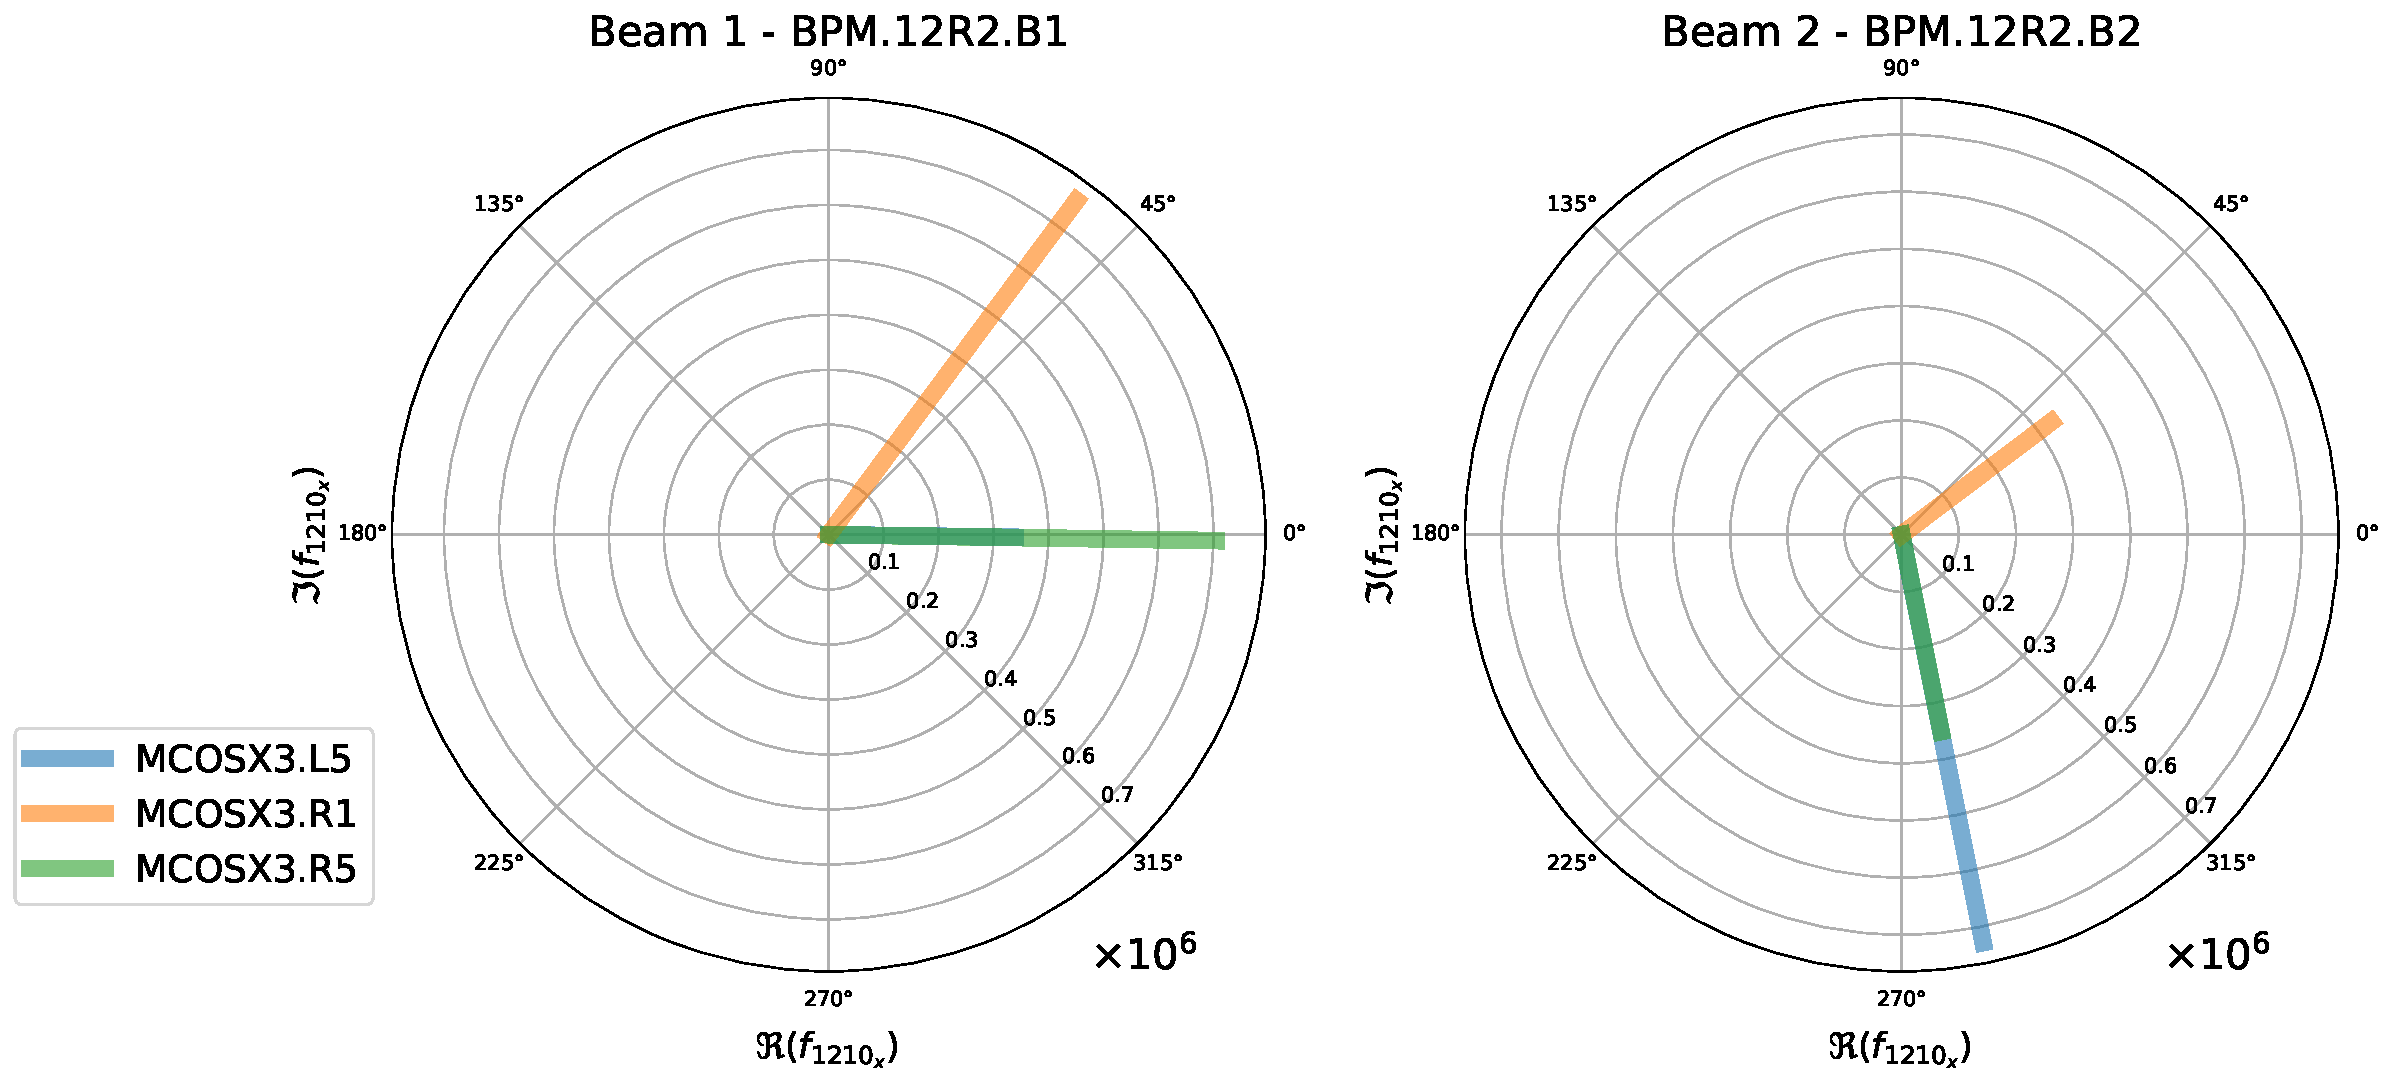
\includegraphics[width=\textwidth]{./images/orthogonal_a4_inj_f1210_x.pdf}
        \caption{$f_{1210,x}$}
    \end{subfigure}
    \caption{Simulated RDTs response of the available skew octupolar correctors at top energy.  Each
    corrector is powered at $J_4 = 1 [\text{m}^{-4}]$. The orthogonality of R1 and L5/R5 allows to
    independently control the real and imaginary parts.}
    \label{fig:skew_octupolar:response_correctors_polar}
\end{figure}



%-----------------------------
%         Correction
%-----------------------------
\subsection{\review{Measurements and Corrections}}

Initial measurements of the machine at top energy ($\beta^*=30$cm) without any skew octupolar
correctors were done during an MD slot in 2022 to determine the level of the RDTs before being able
to correct them. Those measurements were made at natural tunes of $Q_x = 0.285$ and $Q_y = 0.292$.
The driven tunes were set to $\Delta Q_x = -0.008$ and $\Delta Q_y = 0.01$. This selection of tunes
has proven to be appropriate for measuring skew octupolar RDTs. The Landau octupoles were powered
off during the measurements. 

The corrections were computed via the previously detailed response matrix and are shown in
\cref{tab:skew_octupolar:correction_strengths}. These have then been applied during 2023's
commissioning and later on kept for operation. The RDT levels of the bare machine and with these
corrections are shown in \cref{fig:skew_octupolar:corrections_vs_bare}. It can be observed that both
RDT amplitudes are reduced, with the exception of $f_{1210,x}$ for Beam 2, which stays constant.
The reduction of RDT amplitude is comparable to those obtained in 2018, where the same RDT for Beam
2 did neither improve or worsen.


\begin{table}[!htb]
    \centering
    \begin{tabular}{lr}
      \toprule
      Corrector    &    Strength $[\text{m}^{-4}]$ \\
      \midrule
      MCOSX3.L1    &                —  \\
      MCOSX3.R1    &           $-0.50$ \\
      MCOSX3.L5    &           $ 0.42$ \\
      MCOSX3.R5    &           $-0.01$ \\
      \bottomrule
    \end{tabular}
    \caption{Computed corrections for skew octupolar RDTs at top energy. The corrector L1 has been 
    broken for several years and can not be used.}
    \label{tab:skew_octupolar:correction_strengths}
\end{table}
 
\begin{figure}[!htb]
    \centering
    \begin{subfigure}{0.49\textwidth}
        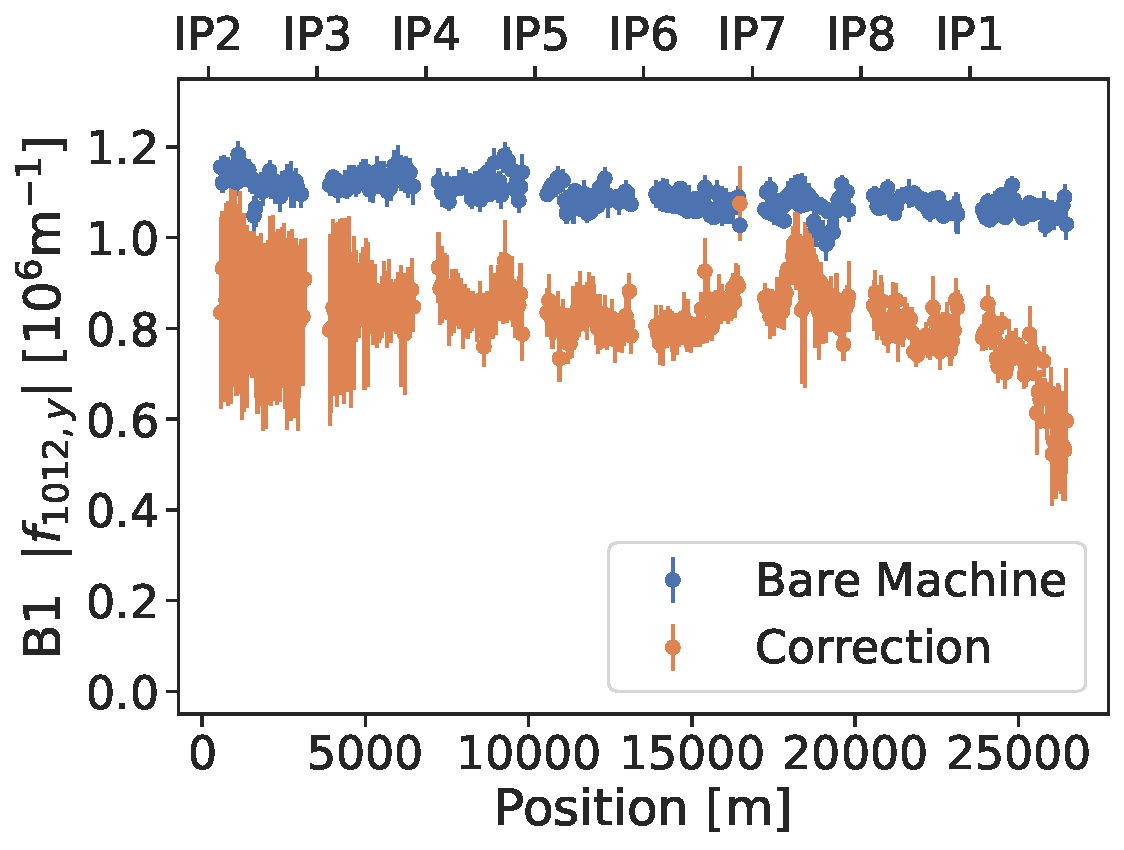
\includegraphics[width=\textwidth]{./images/f1012_b1.pdf}
        \caption{$f_{1012,y}$ Beam 1}
    \end{subfigure}
    \hfill
    \begin{subfigure}{0.49\textwidth}
        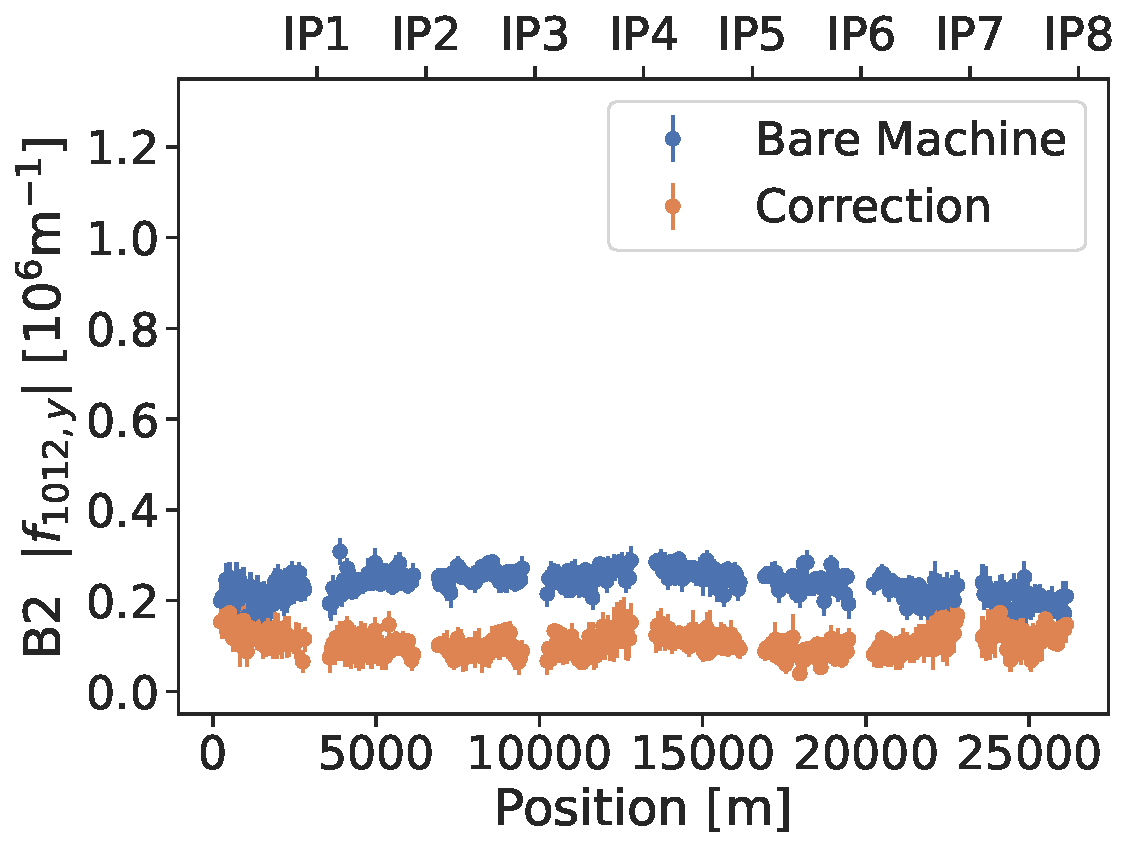
\includegraphics[width=\textwidth]{./images/f1012_b2.pdf}
        \caption{$f_{1012,y}$ Beam 2}
    \end{subfigure}
    %
    \par\bigskip 
    % 
    \begin{subfigure}{0.49\textwidth}
        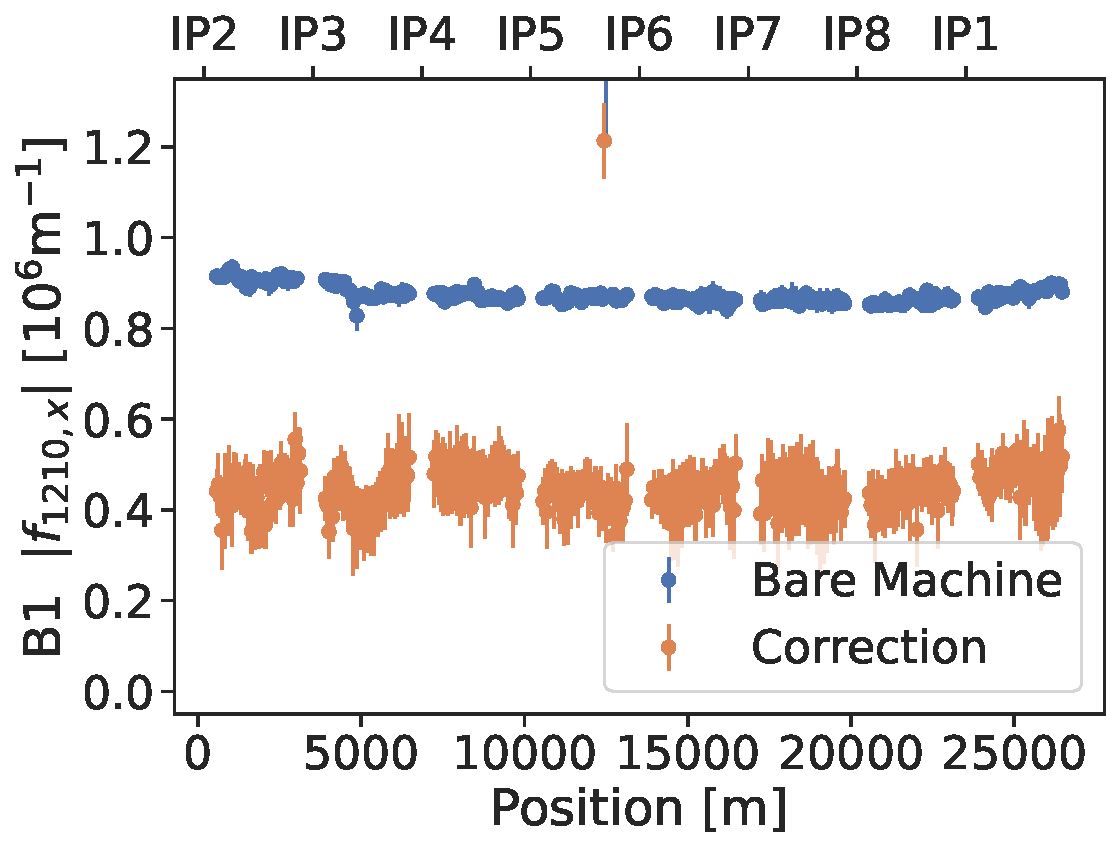
\includegraphics[width=\textwidth]{./images/f1210_b1.pdf}
        \caption{$f_{1210,x}$ Beam 1}
    \end{subfigure}
    \hfill
    \begin{subfigure}{0.49\textwidth}
        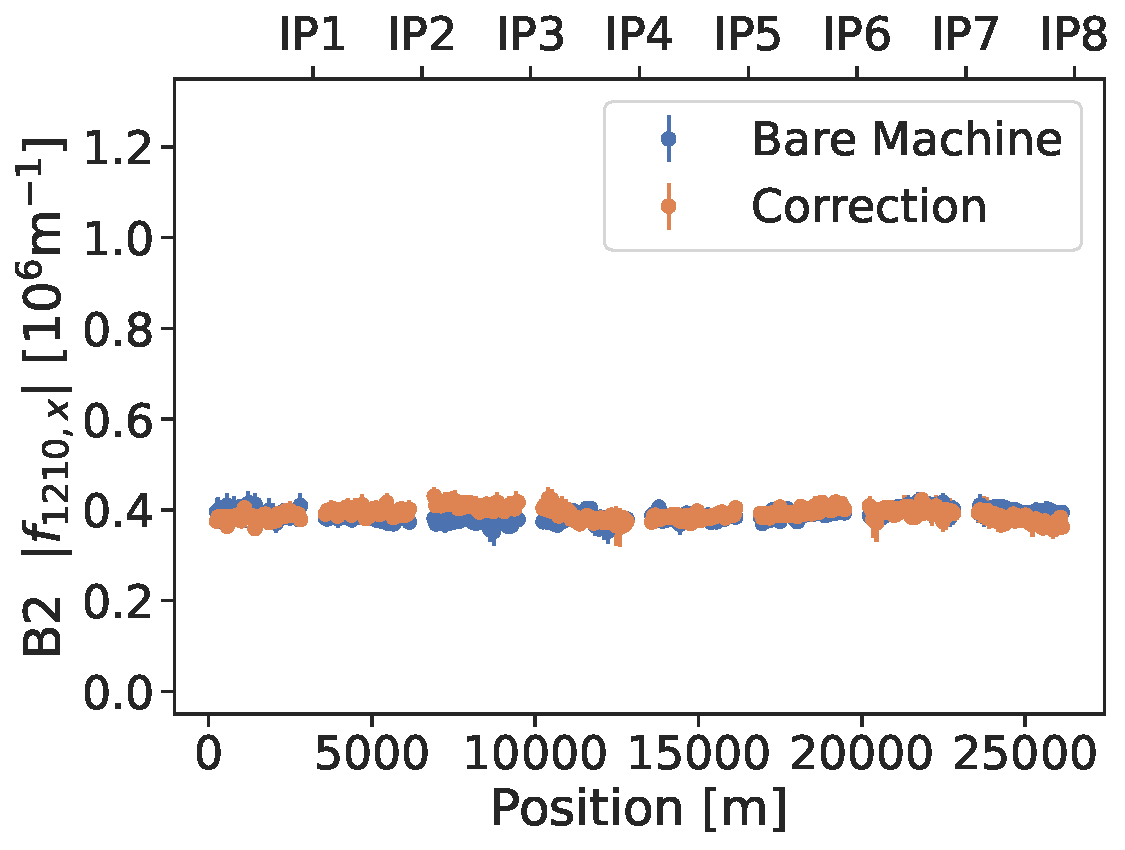
\includegraphics[width=\textwidth]{./images/f1210_b2.pdf}
        \caption{$f_{1210,x}$ Beam 2}
    \end{subfigure}
    \caption{Measured skew octupolar RDTs at top energy and $\beta^*=30\text{cm}$ before and after
    correction. A reduction if observed for all but one RDT in Beam 2.} 
    \label{fig:skew_octupolar:corrections_vs_bare}
\end{figure}






%=============================
%    Landau Contribution
%=============================
% https://indico.cern.ch/event/1351567/contributions/5708754/attachments/2773145/4832599/2023-12-15_MO_Roll_Coupling_complete.pdf
\FloatBarrier
\section{\review{Landau Octupoles Contribution}}


%-----------------------------
%        Introduction
%-----------------------------
\subsection{\review{Introduction}}

During the 2023 commissioning, measurements were taken at injection energy with different strengths
of Landau octupoles, where an unexpected shift in the skew octupolar RDTs was observed. Subsequent
measurements were conducted to better understand and characterize this contribution of normal
octupoles to skew octupolar fields. These new measurements were taken during an MD slot in September
2023 and focused on varying the strengths of the Landau octupoles to $-1K_4$, $\pm2 K_4$, $5K_4$.
All measurements were taken at injection energy at tunes of $Q_x = 0.275$, $Q_y = 0.293$ and
AC-Dipole deltas of $\Delta Q_x = -0.01$ and $\Delta Q_y = -0.011$. Although both beams were
measured, this section focuses on Beam 1 to preliminarily investigate the matter.  The following
\cref{fig:skew_octupolar:mo_different_levels_meas} illustrates the difference in amplitude of the
RDT $f_{1012}$ with these varying strengths.
\Cref{fig:skew_octupolar:mo_meas_vs_sim_+2} on the other hand shows the measured and simulated shift
of the same RDT from $0K_4$ to $+2K_4$. It is evident that simulations including normal and skew 
octupolar field errors are not enough to explain the behaviour observed in the measurements.

\begin{figure}[!htb]
    \centering
    \begin{subfigure}{0.8\textwidth}
        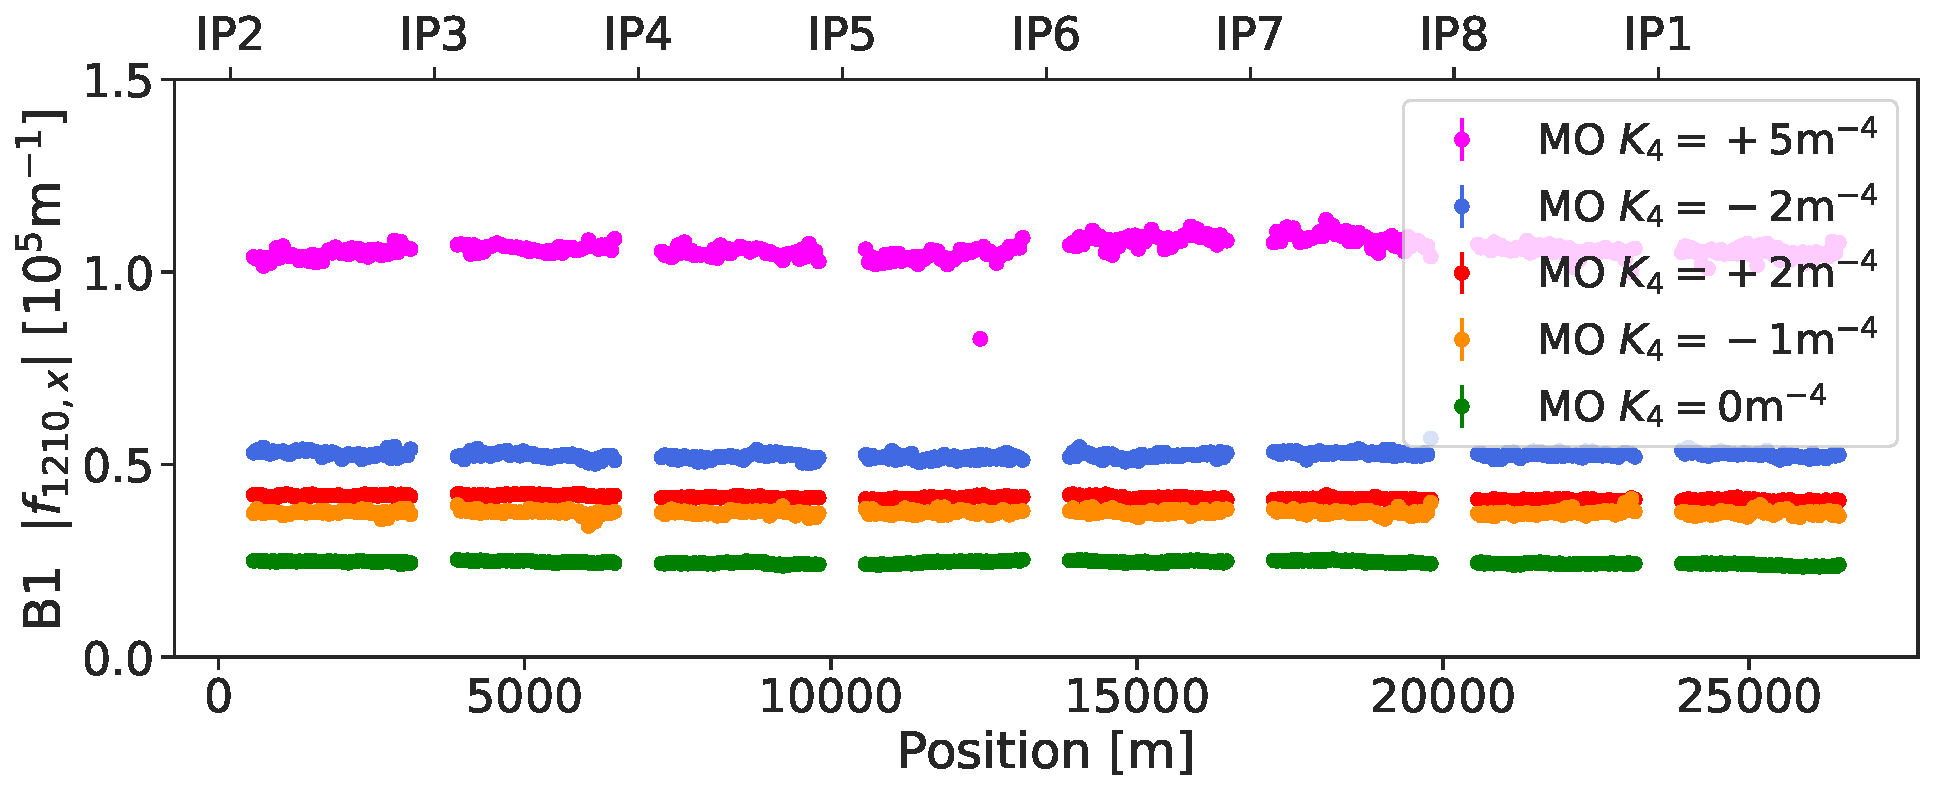
\includegraphics[width=\textwidth]{./images/skew_octupoles/f1210_AMP_all_measurements.pdf}
    \end{subfigure}
    \caption{Unexpected difference of skew octupolar RDT amplitudes with varying Landau octupoles
    strengths.}
    \label{fig:skew_octupolar:mo_different_levels_meas}
\end{figure}

\begin{figure}[!htb]
    \centering
    \begin{subfigure}{0.8\textwidth}
        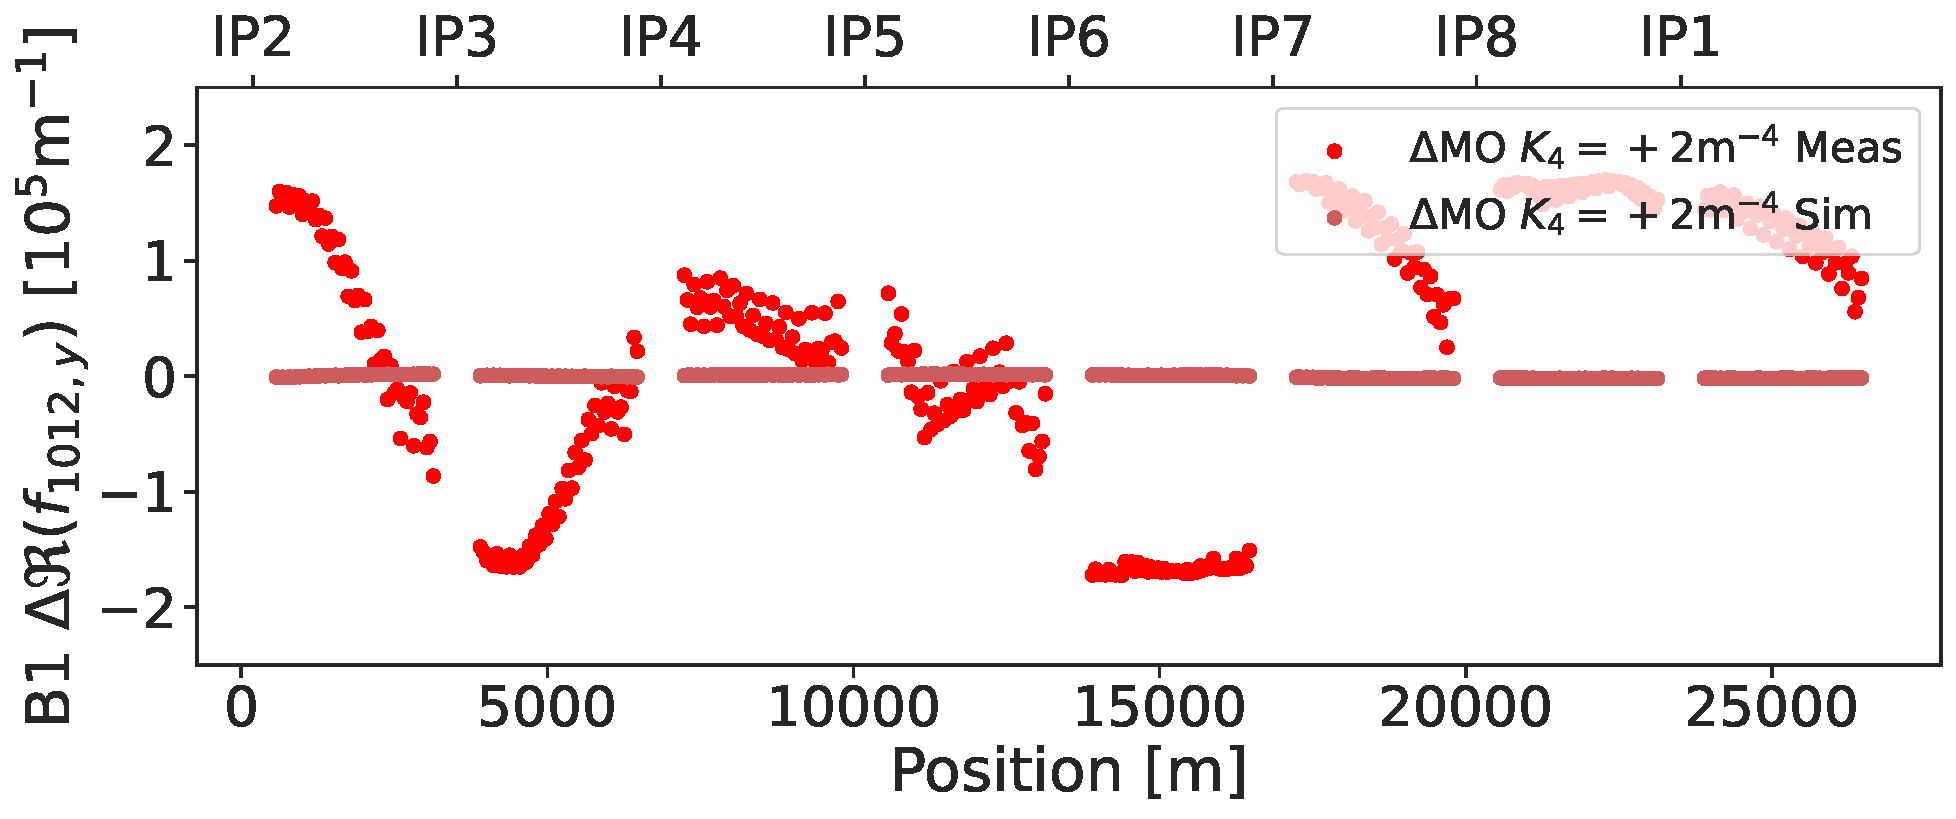
\includegraphics[width=\textwidth]{./images/skew_octupoles/f1012_meas_vs_sim_0shift.pdf}
        %\caption{$f_{1012,y}$}
    \end{subfigure}
    \caption{Measured and simulated shift of skew octupolar RDT after increase of Landau octupoles
    strength from zero. It is apparent that the shift in measurement is not replicated by the
    simulation.}
    \label{fig:skew_octupolar:mo_meas_vs_sim_+2}
\end{figure}



%-----------------------------
%        Misalignments
%-----------------------------
\subsection{\review{Misalignments}}

Magnet misalignments, more specifically roll errors, can generate skew magnetic fields instead of
the expected normal ones. To determine if this could explain the behaviour observed in measurements,
a tracking simulation was conducted with and without roll errors applied to the Landau octupoles.
The resulting RDTs reveal an imperceptible difference, unable to account for  the previously seen
shifts. The real part of the RDT $f_{1012}$ is shown in \cref{fig:skew_octupolar:sim_misalign},
with similar results seen in the other component and in $f_{1210}$.

\begin{figure}[!htb]
    \centering
    \begin{subfigure}{0.8\textwidth}
        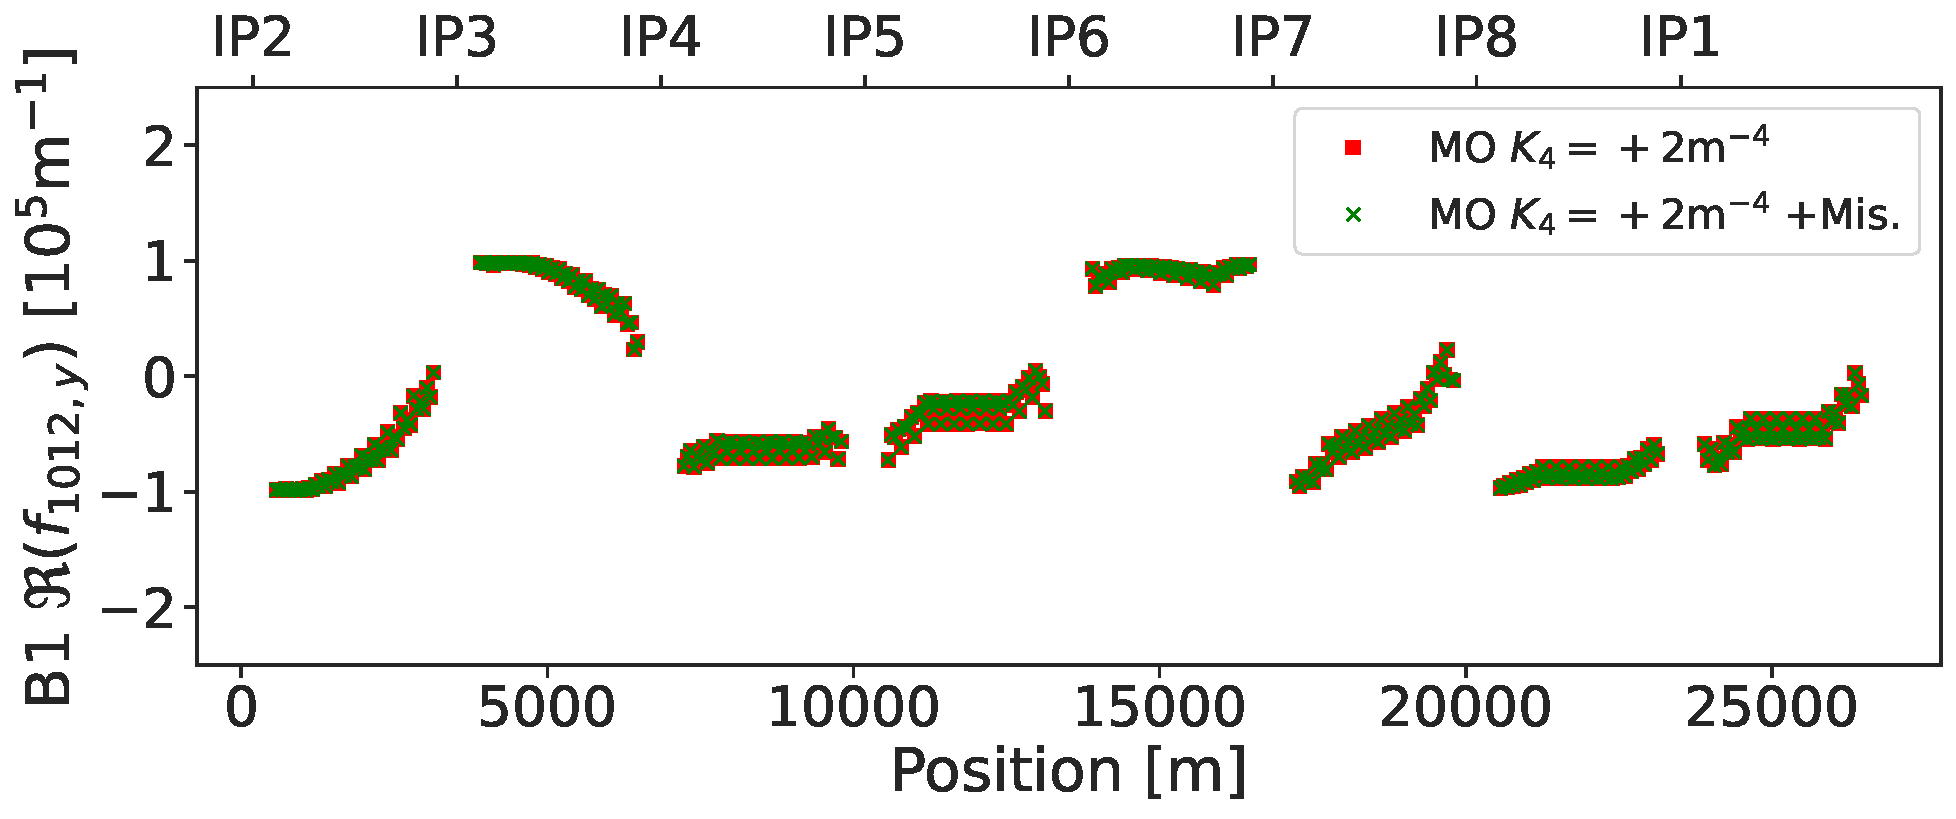
\includegraphics[width=\textwidth]{./images/skew_octupoles/f1012_misalign_REAL.pdf}
        %\caption{$f_{1012,y}$}
    \end{subfigure}
    \caption{Simulated skew octupolar RDT with normal and skew octupolar errors and Landau octupoles
    powered. One simulation includes further alignment errors on the Landau octupoles. No 
    significant difference is observed between the two.}
    \label{fig:skew_octupolar:sim_misalign}
\end{figure}



%-----------------------------
%        Coupling
%-----------------------------
\subsection{\review{Coupling}}

As misalignments could not explain the discrepancy, simulations were first run with varying values
of coupling at a fixed octupolar strength, allowing to gage the impact of coupling only.
\Cref{appendix:transfer_map:skew_quadrupole_and_octupole} details how coupling, in the form of a
skew quadrupole, combined with a normal octupole can generate skew quadrupolar-like fields.
The resulting RDT $f_{1012}$ is shown in \cref{fig:skew_octupolar:sim_coupling}, a similar trend is
observed for $f_{1210}$.
The presented $C^{-}$ values are commonly seen in operation and well below that of the
tolerances of the design of the LHC~\cite{bruning_lhc_2004}. As coupling increases, the skew
octupolar RDTs are expected to be significantly altered.

\begin{figure}[!htb]
    \centering
    \begin{subfigure}{0.8\textwidth}
        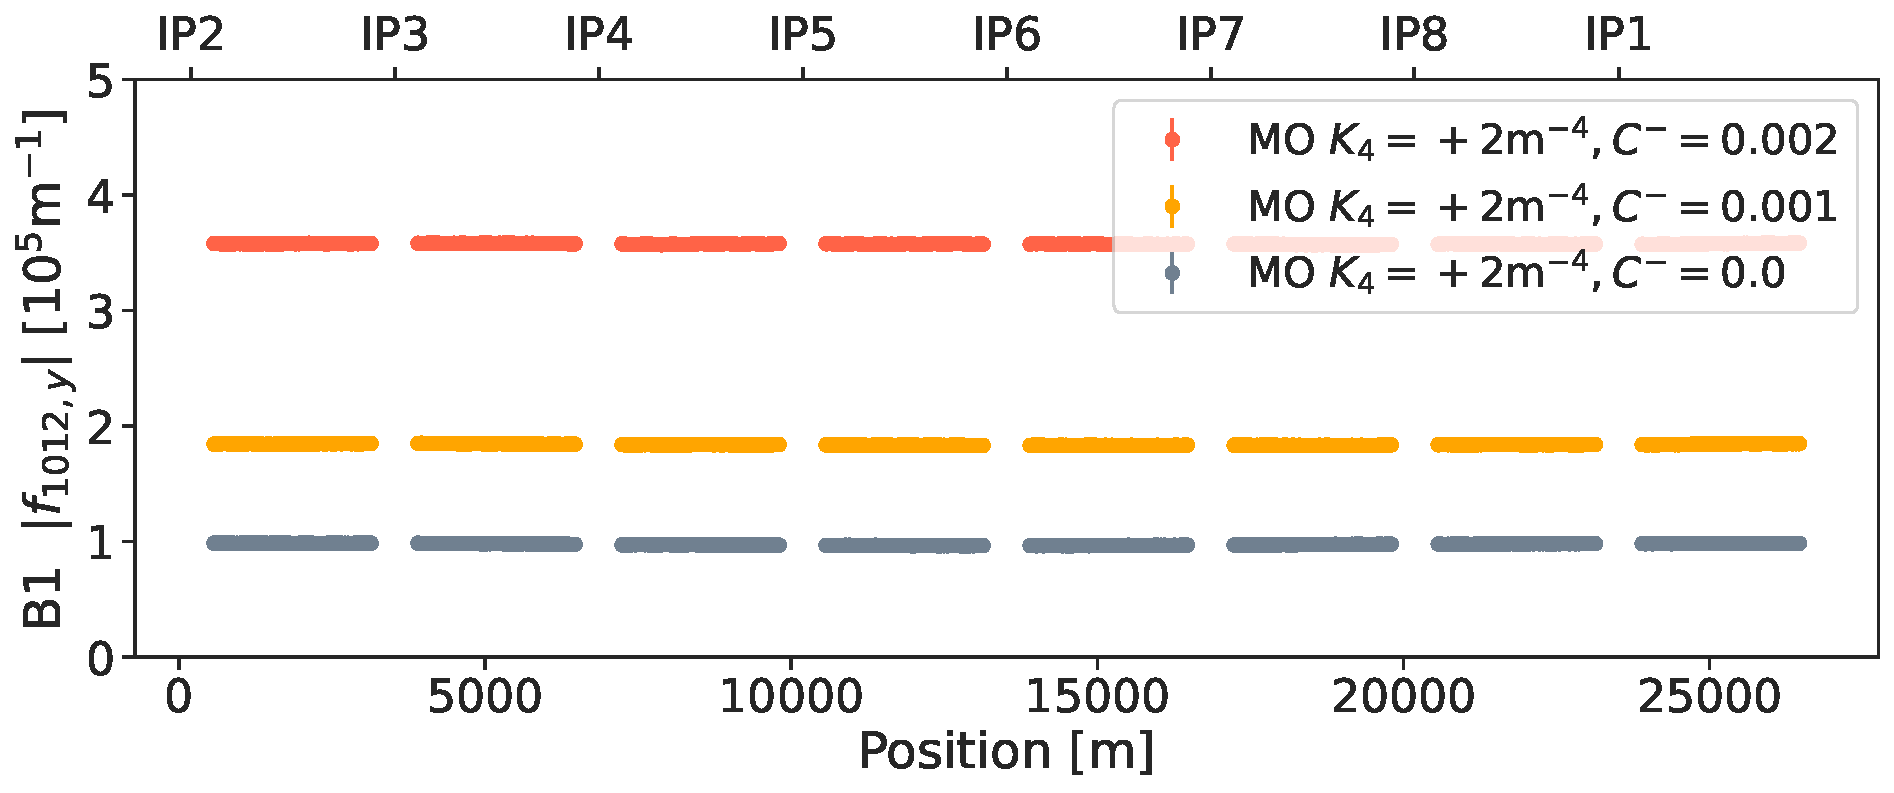
\includegraphics[width=\textwidth]{./images/skew_octupoles/f1012_coupling_sim_AMP.pdf}
    \end{subfigure}
    \caption{Simulated skew octupolar RDT with fixed Landau octupole strength but varying coupling.
    Selected coupling values are often seen in operation.}
    \label{fig:skew_octupolar:sim_coupling}
\end{figure}



%-----------------------------
%          Responses
\FloatBarrier
\subsubsection{\review{Responses with Coupling}}

\begin{table}[!htb]
    \centering
    \begin{tabular}{cccc}
    \toprule
    &&\multicolumn{2}{c}{Rel. Diff. [\%]} \\
    \cmidrule{3-4}
    $K_4$ $[\text{m}^{-4}]$ & RDT & Real & Imag. \\
    \midrule
    \multirow{2}{*}{+5}
     & $f_{1210}$ & 6 & 6  \\
     & $f_{1012}$ & 12  & 11 \\[0.5em]
    \multirow{2}{*}{+2}
     & $f_{1210}$ & 32  & 34  \\
     & $f_{1012}$ & 36  & 36  \\[0.5em]
    \multirow{2}{*}{-1}
     & $f_{1210}$ & 26 & 25 \\
     & $f_{1012}$ & 21 & 20 \\[0.5em]
    \multirow{2}{*}{-2}
     & $f_{1210}$ & 19  & 17  \\
     & $f_{1012}$ & 21 & 20 \\
    \bottomrule
    \end{tabular}
    \caption{Relative difference between measured and simulated RDT shift induced by the
    Landau octupoles in presence of coupling. Real parts are illustrated in
    \cref{fig:skew_octupolar:response_meas_sim_coupling}.}
    \label{tab:skew_octupolar:rms_ratios}
\end{table}

After having demonstrated that coupling could significantly contribute to the creation of skew
octupolar fields with normal octupoles, additional simulations were performed matching the measured
coupling for each set of measurements. The shift in real part of the RDTs $f_{1012}$ and $f_{1210}$
is shown in \cref{fig:skew_octupolar:response_meas_sim_coupling}, with a similar pattern observed
for the imaginary part. The relative RMS deviation between simulations and measurements is given
for each set of strengths and RDTs in \cref{tab:skew_octupolar:rms_ratios}.

It can be observed that simulations and measurements for positive strengths ($K_4=2$ and $K_4=5$) 
are now in good agreement. This suggests that the primary contribution to the skew octupolar RDTs
can be attributed to the Landau octupoles and coupling. The relative deviation between measurement
and simulation can be explained by the sensitivity to the coupling. A difference of $10^{-4}$ units 
is enough to be noticeable, making accurate reproduction of skew octupolar RDTs not trivial.
It is important to note that measurements of $f_{1012}$ with \textit{negative} strength show a
response opposite to what is predicted by simulations while $f_{1210}$ agrees well. This behaviour
is not yet understood and requires further investigation.

\begin{figure}[!htb]
    \centering
    \begin{subfigure}{0.47\textwidth}
        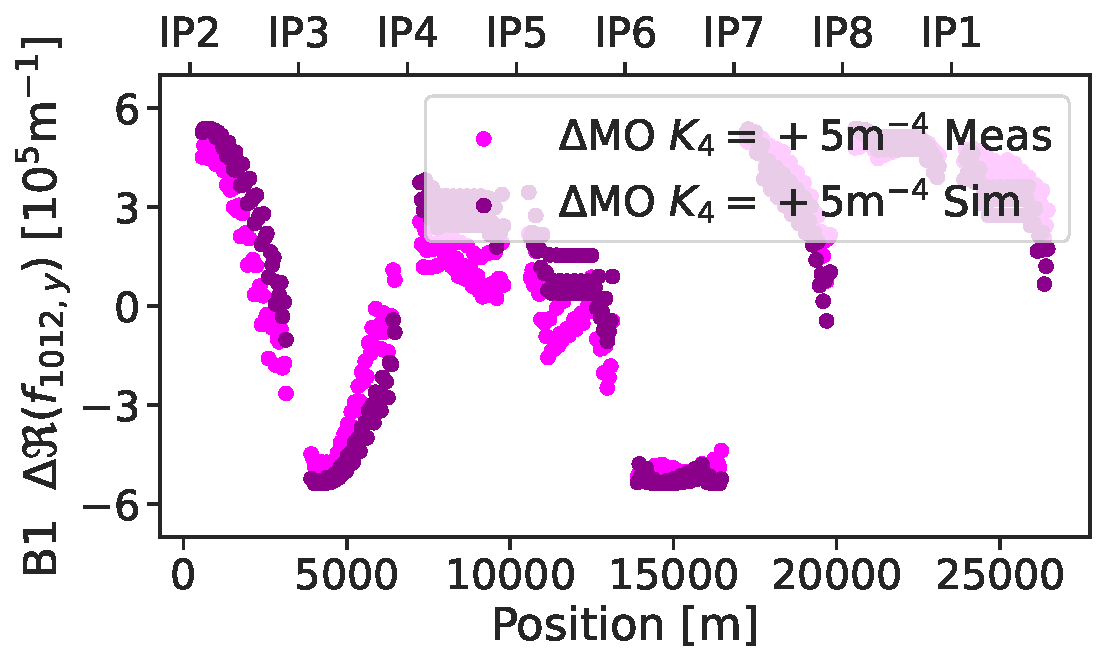
\includegraphics[width=\textwidth]{./images/skew_octupoles/responses_coupling/f1012_response_meas_sim_+5_REAL_smoll.pdf}
        %\caption{$f_{1012,y}$ for $K_4 = +5$}
    \end{subfigure}
    \hfill
    \begin{subfigure}{0.47\textwidth}
        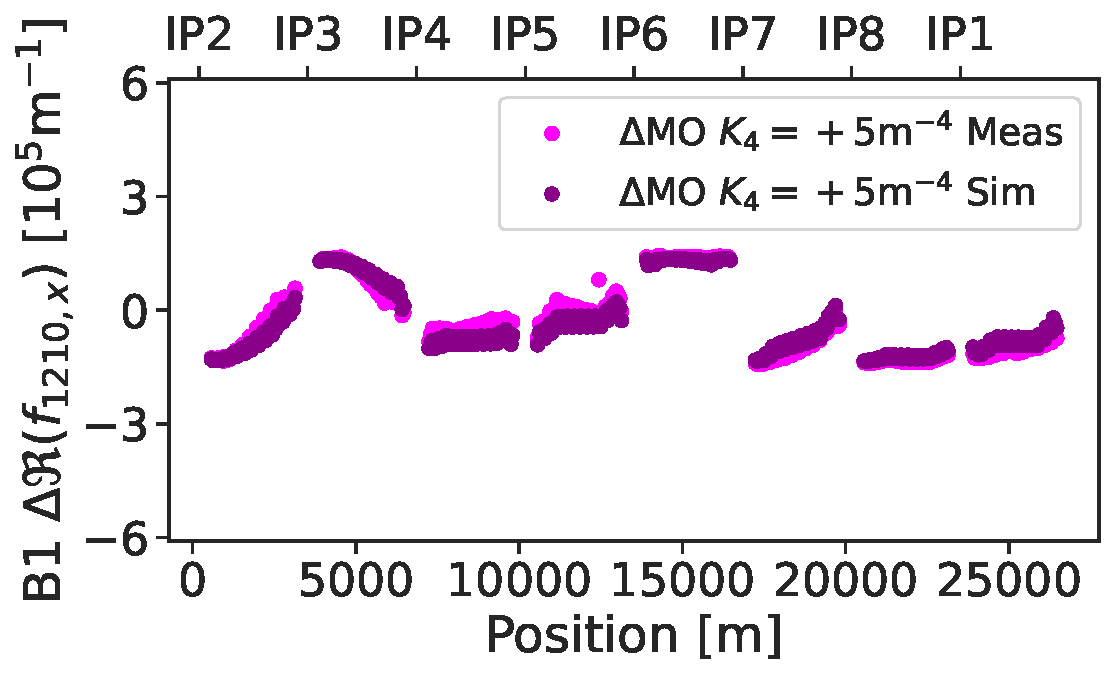
\includegraphics[width=\textwidth]{./images/skew_octupoles/responses_coupling/f1210_response_meas_sim_+5_REAL_smoll.pdf}
        %\caption{$f_{1210,x}$ for $K_4 = +5$}
    \end{subfigure}
    %
    \par\medskip 
    %
    \begin{subfigure}{0.47\textwidth}
        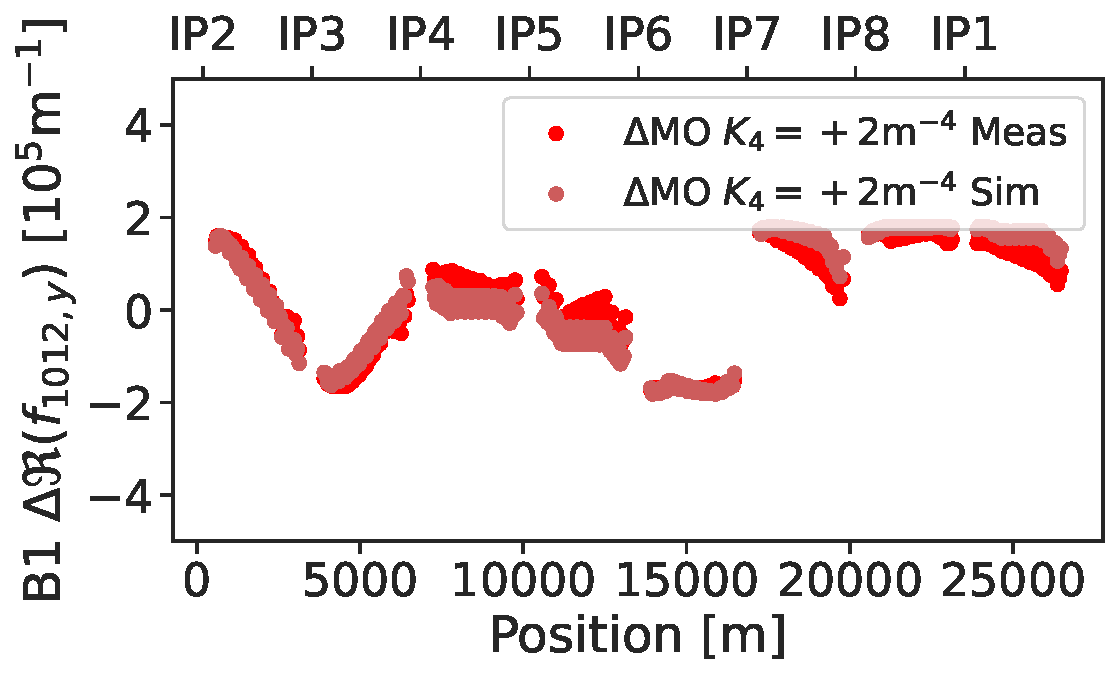
\includegraphics[width=\textwidth]{./images/skew_octupoles/responses_coupling/f1012_response_meas_sim_+2_REAL_smoll.pdf}
        %\caption{$f_{1012,y}$ for $K_4 = +2$}
    \end{subfigure}
    \hfill
    \begin{subfigure}{0.47\textwidth}
        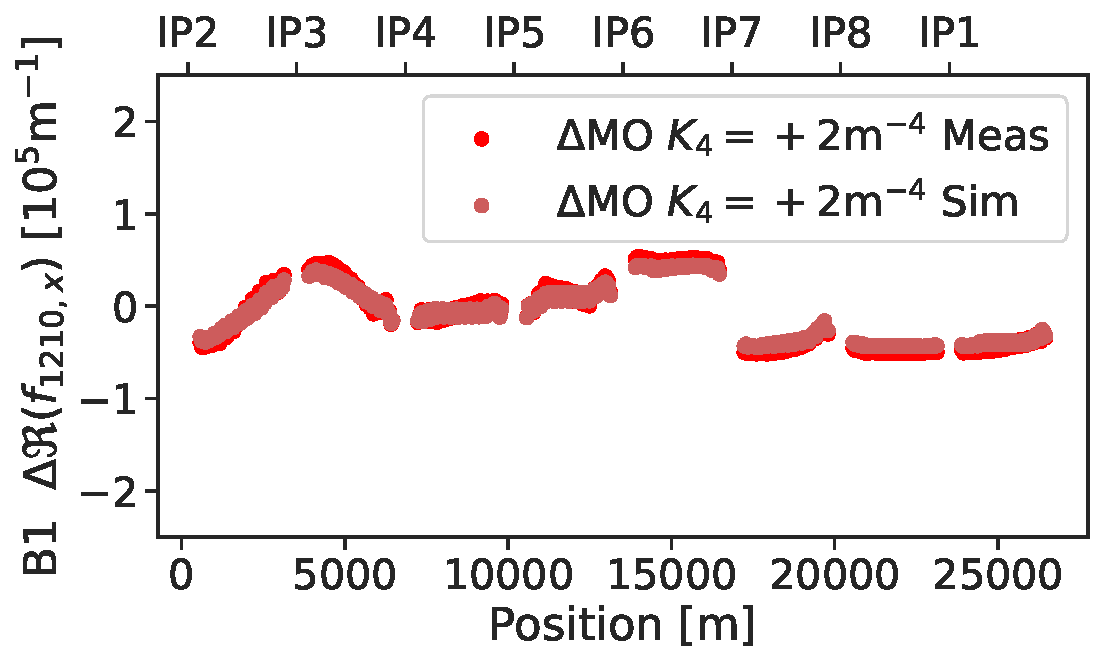
\includegraphics[width=\textwidth]{./images/skew_octupoles/responses_coupling/f1210_response_meas_sim_+2_REAL_smoll.pdf}
        %\caption{$f_{1210,x}$ for $K_4 = +2$}
    \end{subfigure}
    %
    \par\medskip 
    %
    \begin{subfigure}{0.47\textwidth}
        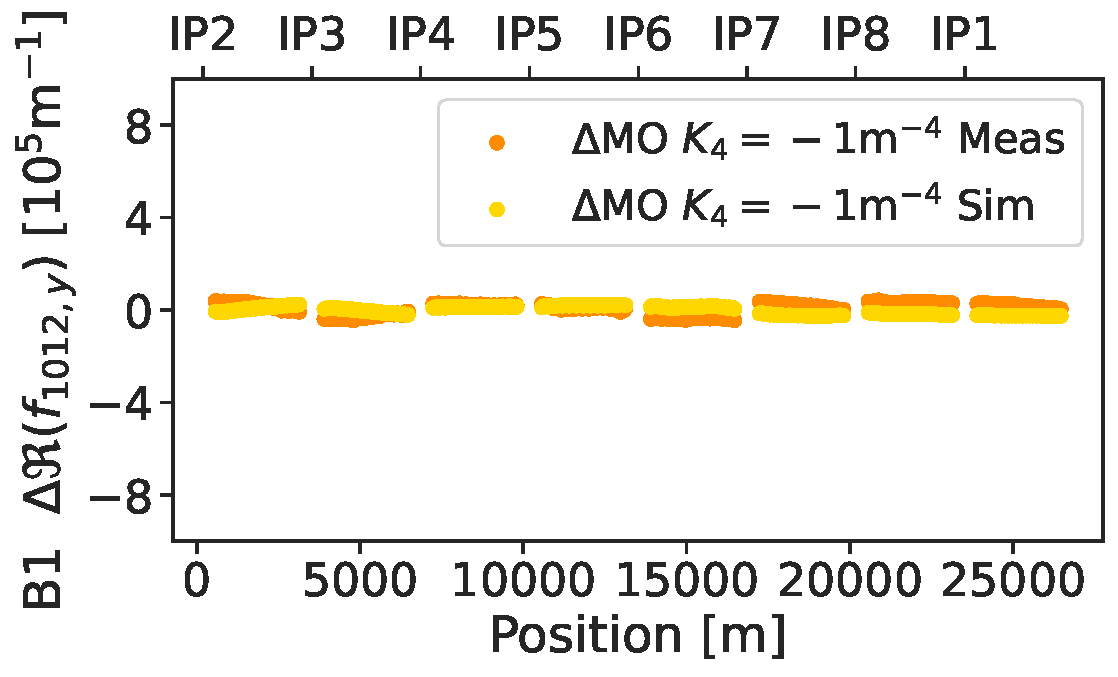
\includegraphics[width=\textwidth]{./images/skew_octupoles/responses_coupling/f1012_response_meas_sim_-1_REAL_smoll.pdf}
        %\caption{$f_{1012,y}$ for $K_4 = -1$}
    \end{subfigure}
    \hfill
    \begin{subfigure}{0.47\textwidth}
        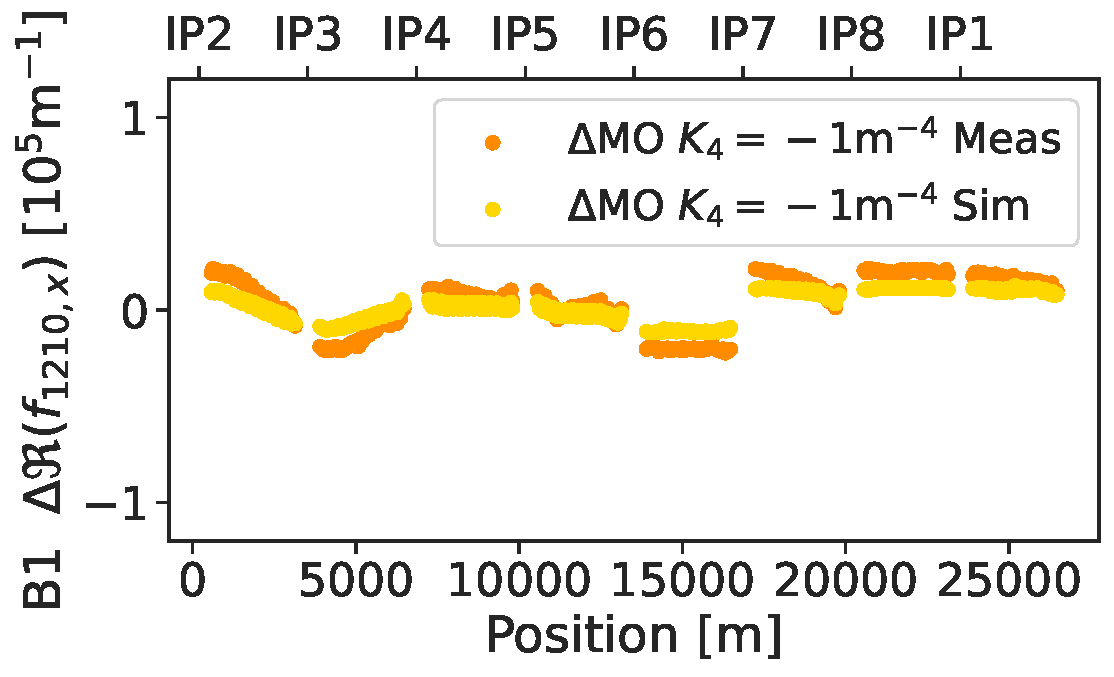
\includegraphics[width=\textwidth]{./images/skew_octupoles/responses_coupling/f1210_response_meas_sim_-1_REAL_smoll.pdf}
        %\caption{$f_{1210,x}$ for $K_4 = -1$}
    \end{subfigure}
    %
    \par\medskip
    %
    \begin{subfigure}{0.47\textwidth}
        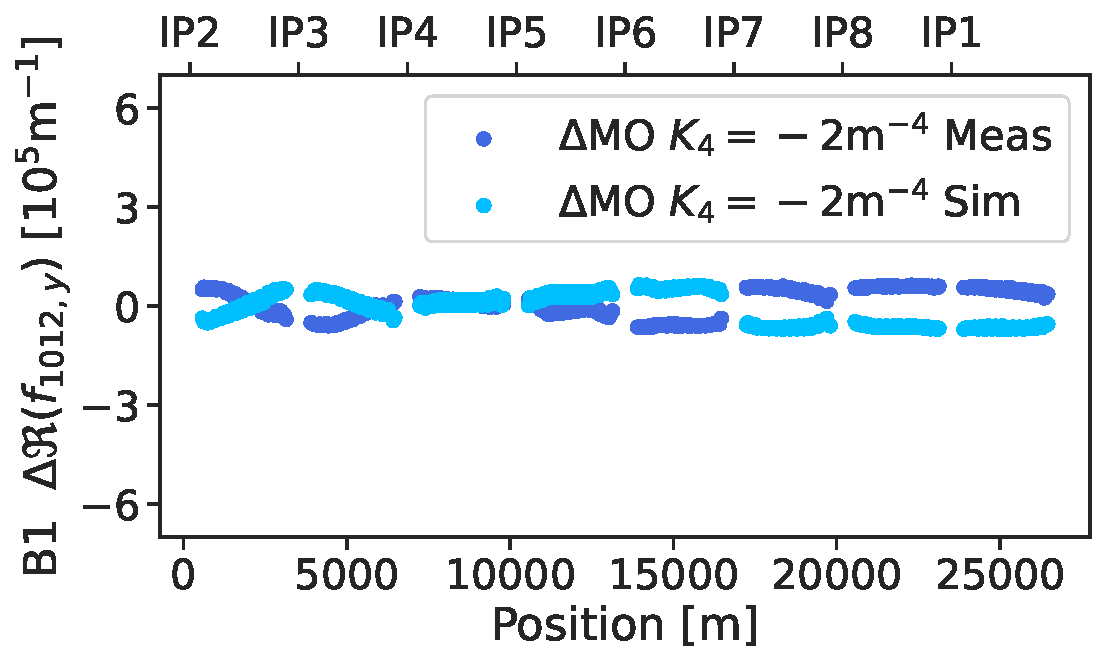
\includegraphics[width=\textwidth]{./images/skew_octupoles/responses_coupling/f1012_response_meas_sim_-2_REAL_smoll.pdf}
        %\caption{$f_{1012,y}$ for $K_4 = -2$}
    \end{subfigure}
    \hfill
    \begin{subfigure}{0.47\textwidth}
        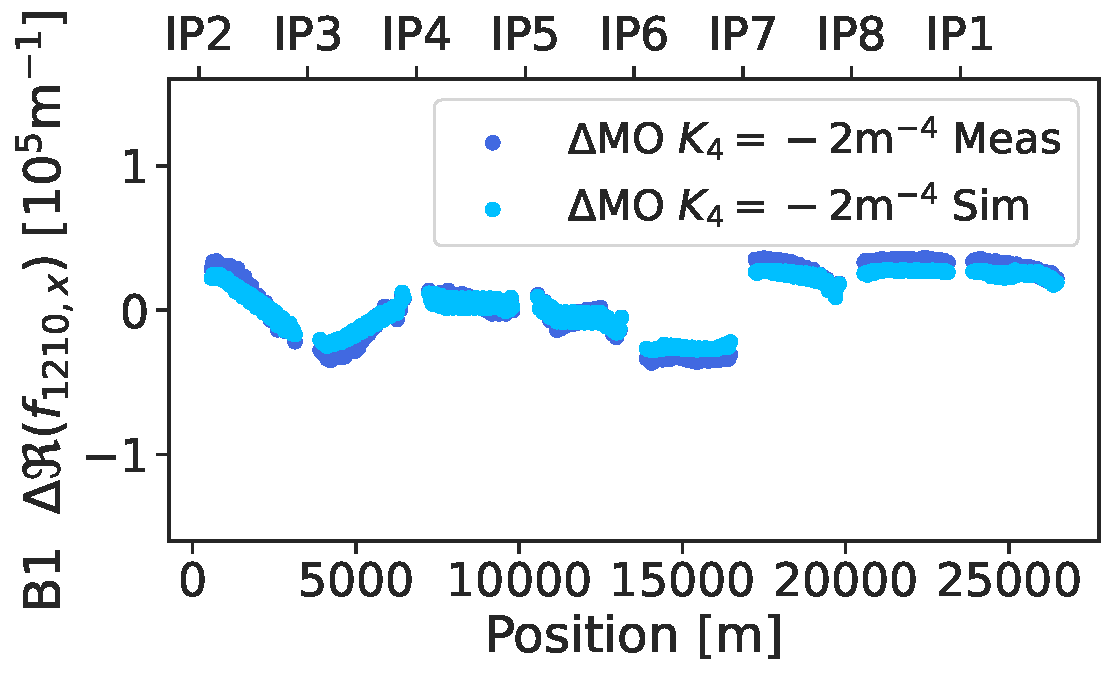
\includegraphics[width=\textwidth]{./images/skew_octupoles/responses_coupling/f1210_response_meas_sim_-2_REAL_smoll.pdf}
        %\caption{$f_{1210,x}$ for $K_4 = -2$}
    \end{subfigure}
    \caption{Measured and simulated real part shift of skew octupolar RDTs induced by Landau
    octupoles in presence of coupling at injection energy. Left column shows $f_{1012}$ while right
    shows $f_{1210}$. The vertical scale is adjusted for each plot to highlight the agreement of the 
    simulations.}
    \label{fig:skew_octupolar:response_meas_sim_coupling}
\end{figure}


% Imaginary Parts
%\begin{figure}[!htb]
%    \centering
%    \begin{subfigure}{0.47\textwidth}
%        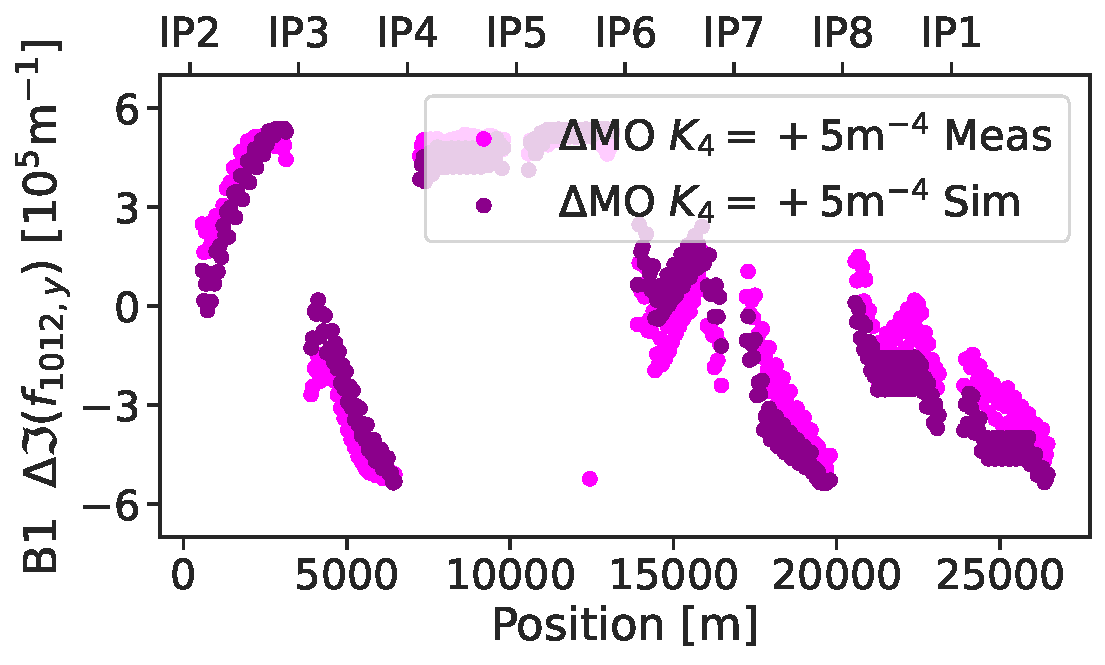
\includegraphics[width=\textwidth]{./images/skew_octupoles/responses_coupling/f1012_response_meas_sim_+5_IMAG_smoll.pdf}
%        %\caption{$f_{1012,y}$ for $K_4 = +5$}
%    \end{subfigure}
%    \hfill
%    \begin{subfigure}{0.47\textwidth}
%        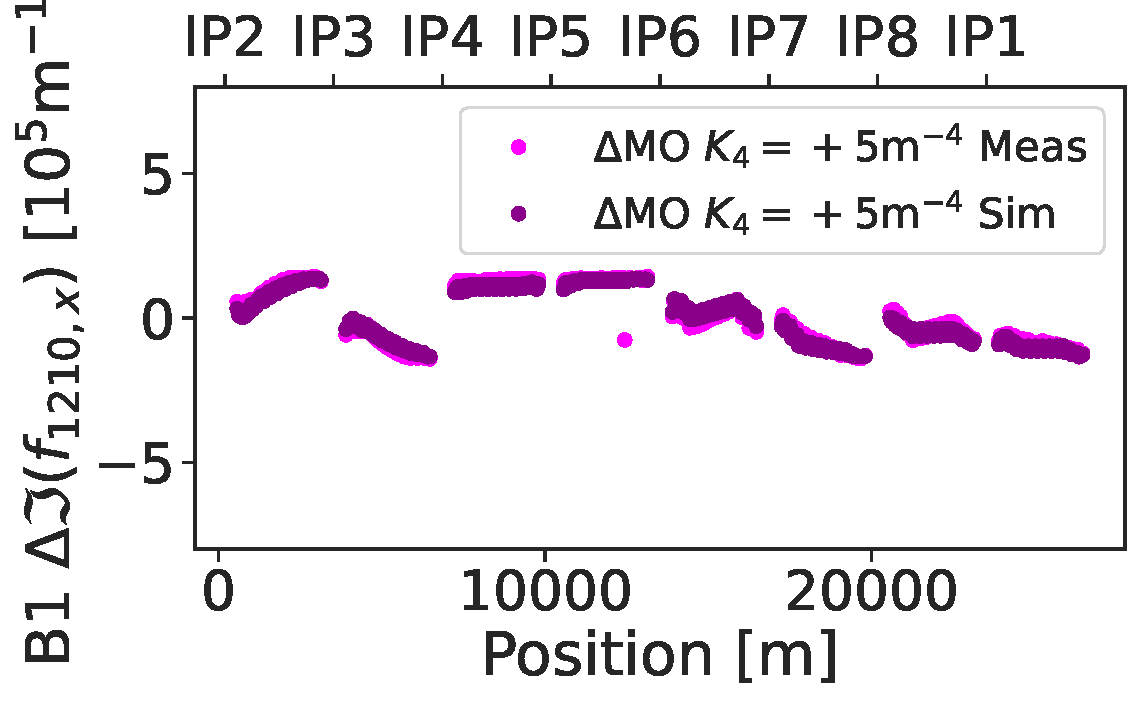
\includegraphics[width=\textwidth]{./images/skew_octupoles/responses_coupling/f1210_response_meas_sim_+5_IMAG_smoll.pdf}
%        %\caption{$f_{1210,x}$ for $K_4 = +5$}
%    \end{subfigure}
%    %
%    \par\medskip 
%    %
%    \begin{subfigure}{0.47\textwidth}
%        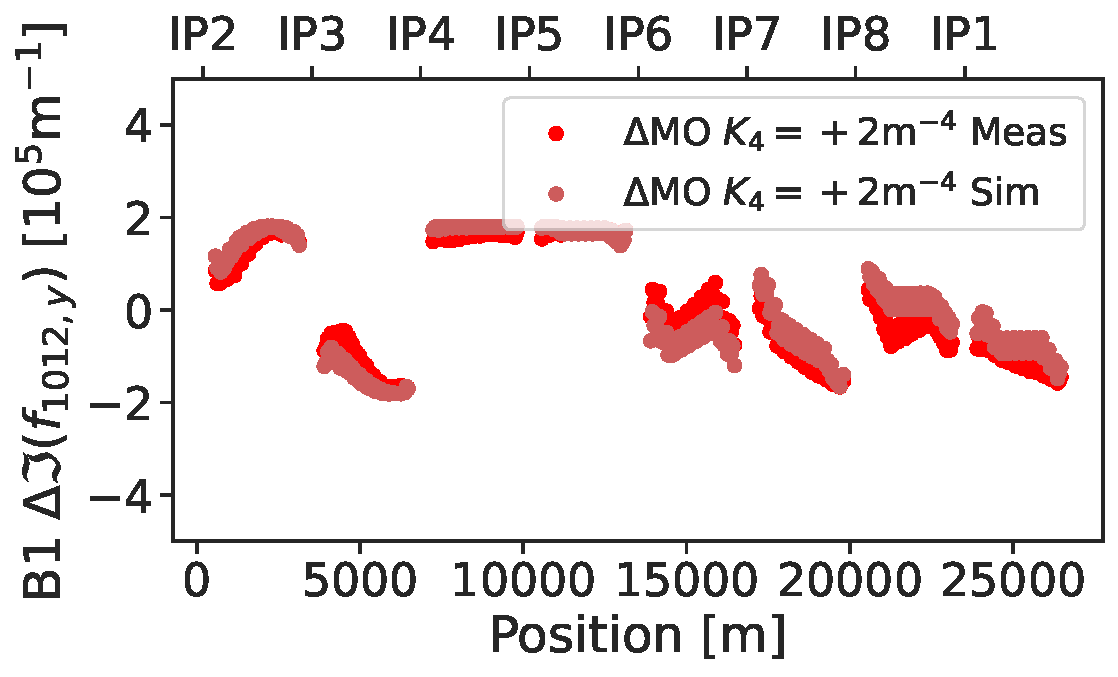
\includegraphics[width=\textwidth]{./images/skew_octupoles/responses_coupling/f1012_response_meas_sim_+2_IMAG_smoll.pdf}
%        %\caption{$f_{1012,y}$ for $K_4 = +2$}
%    \end{subfigure}
%    \hfill
%    \begin{subfigure}{0.47\textwidth}
%        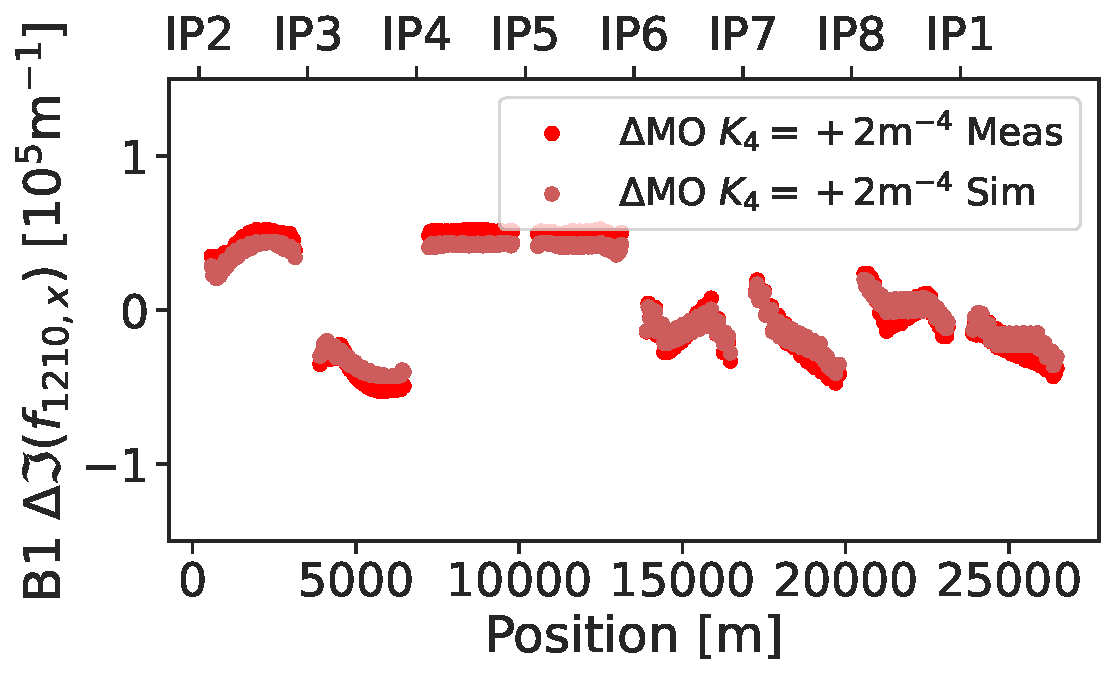
\includegraphics[width=\textwidth]{./images/skew_octupoles/responses_coupling/f1210_response_meas_sim_+2_IMAG_smoll.pdf}
%        %\caption{$f_{1210,x}$ for $K_4 = +2$}
%    \end{subfigure}
%    %
%    \par\medskip 
%    %
%    \begin{subfigure}{0.47\textwidth}
%        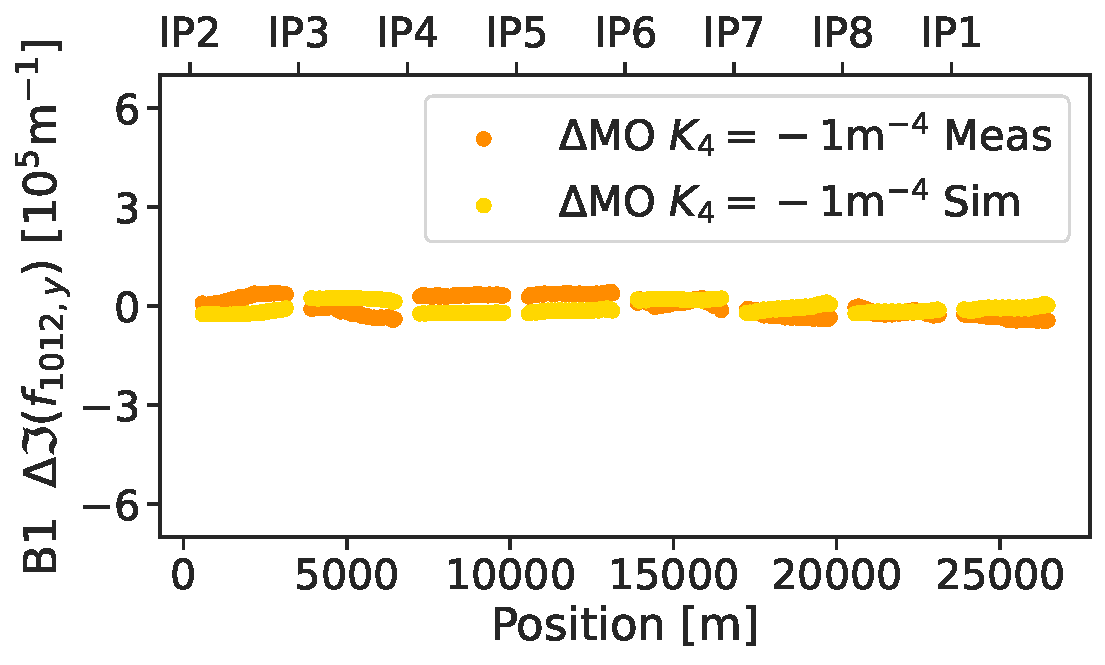
\includegraphics[width=\textwidth]{./images/skew_octupoles/responses_coupling/f1012_response_meas_sim_-1_IMAG_smoll.pdf}
%        %\caption{$f_{1012,y}$ for $K_4 = -1$}
%    \end{subfigure}
%    \hfill
%    \begin{subfigure}{0.47\textwidth}
%        \includegraphics[width=\textwidth]{./images/skew_octupoles/responses_coupling/f1210_response_meas_sim_-1_IMAG_smoll.pdf}
%        %\caption{$f_{1210,x}$ for $K_4 = -1$}
%    \end{subfigure}
%    %
%    \par\medskip
%    %
%    \begin{subfigure}{0.47\textwidth}
%        \includegraphics[width=\textwidth]{./images/skew_octupoles/responses_coupling/f1012_response_meas_sim_-2_IMAG_smoll.pdf}
%        %\caption{$f_{1012,y}$ for $K_4 = -2$}
%    \end{subfigure}
%    \hfill
%    \begin{subfigure}{0.47\textwidth}
%        \includegraphics[width=\textwidth]{./images/skew_octupoles/responses_coupling/f1210_response_meas_sim_-2_IMAG_smoll.pdf}
%        %\caption{$f_{1210,x}$ for $K_4 = -2$}
%    \end{subfigure}
%    \caption{Measured and simulated imaginary part shift of skew octupolar RDTs induced by Landau
%    octupoles in presence of coupling at injection energy. Left column shows $f_{1012}$ while right
%    shows $f_{1210}$.}
%    \label{fig:skew_octupolar:response_meas_sim_coupling_imag}
%\end{figure}


% Constant coupling
%\begin{figure}[!htb]
%    \centering
%    \begin{subfigure}{0.47\textwidth}
%        \includegraphics[width=\textwidth]{./images/skew_octupoles/responses_coupling/f1012_response_meas_sim_+5_REAL_smoll_const_coupling.pdf}
%        %\caption{$f_{1012,y}$ for $K_4 = +5$}
%    \end{subfigure}
%    \hfill
%    \begin{subfigure}{0.47\textwidth}
%        \includegraphics[width=\textwidth]{./images/skew_octupoles/responses_coupling/f1210_response_meas_sim_+5_REAL_smoll_const_coupling.pdf}
%        %\caption{$f_{1210,x}$ for $K_4 = +5$}
%    \end{subfigure}
%    %
%    \par\medskip 
%    %
%    \begin{subfigure}{0.47\textwidth}
%        \includegraphics[width=\textwidth]{./images/skew_octupoles/responses_coupling/f1012_response_meas_sim_+2_REAL_smoll_const_coupling.pdf}
%        %\caption{$f_{1012,y}$ for $K_4 = +2$}
%    \end{subfigure}
%    \hfill
%    \begin{subfigure}{0.47\textwidth}
%        \includegraphics[width=\textwidth]{./images/skew_octupoles/responses_coupling/f1210_response_meas_sim_+2_REAL_smoll_const_coupling.pdf}
%        %\caption{$f_{1210,x}$ for $K_4 = +2$}
%    \end{subfigure}
%    %
%    \par\medskip 
%    %
%    \begin{subfigure}{0.47\textwidth}
%        \includegraphics[width=\textwidth]{./images/skew_octupoles/responses_coupling/f1012_response_meas_sim_-1_REAL_smoll_const_coupling.pdf}
%        %\caption{$f_{1012,y}$ for $K_4 = -1$}
%    \end{subfigure}
%    \hfill
%    \begin{subfigure}{0.47\textwidth}
%        \includegraphics[width=\textwidth]{./images/skew_octupoles/responses_coupling/f1210_response_meas_sim_-1_REAL_smoll_const_coupling.pdf}
%        %\caption{$f_{1210,x}$ for $K_4 = -1$}
%    \end{subfigure}
%    %
%    \par\medskip
%    %
%    \begin{subfigure}{0.47\textwidth}
%        \includegraphics[width=\textwidth]{./images/skew_octupoles/responses_coupling/f1012_response_meas_sim_-2_REAL_smoll_const_coupling.pdf}
%        %\caption{$f_{1012,y}$ for $K_4 = -2$}
%    \end{subfigure}
%    \hfill
%    \begin{subfigure}{0.47\textwidth}
%        \includegraphics[width=\textwidth]{./images/skew_octupoles/responses_coupling/f1210_response_meas_sim_-2_REAL_smoll_const_coupling.pdf}
%        %\caption{$f_{1210,x}$ for $K_4 = -2$}
%    \end{subfigure}
%    \caption{Measured and simulated real part shift of skew octupolar RDTs induced by Landau
%    octupoles in presence of coupling at injection energy. Left column shows $f_{1012}$ while right
%    shows $f_{1210}$.}
%    \label{fig:skew_octupolar:response_meas_sim_coupling}
%\end{figure}
%
%
%% Imaginary Parts
%\begin{figure}[!htb]
%    \centering
%    \begin{subfigure}{0.47\textwidth}
%        \includegraphics[width=\textwidth]{./images/skew_octupoles/responses_coupling/f1012_response_meas_sim_+5_IMAG_smoll_const_coupling.pdf}
%        %\caption{$f_{1012,y}$ for $K_4 = +5$}
%    \end{subfigure}
%    \hfill
%    \begin{subfigure}{0.47\textwidth}
%        \includegraphics[width=\textwidth]{./images/skew_octupoles/responses_coupling/f1210_response_meas_sim_+5_IMAG_smoll_const_coupling.pdf}
%        %\caption{$f_{1210,x}$ for $K_4 = +5$}
%    \end{subfigure}
%    %
%    \par\medskip 
%    %
%    \begin{subfigure}{0.47\textwidth}
%        \includegraphics[width=\textwidth]{./images/skew_octupoles/responses_coupling/f1012_response_meas_sim_+2_IMAG_smoll_const_coupling.pdf}
%        %\caption{$f_{1012,y}$ for $K_4 = +2$}
%    \end{subfigure}
%    \hfill
%    \begin{subfigure}{0.47\textwidth}
%        \includegraphics[width=\textwidth]{./images/skew_octupoles/responses_coupling/f1210_response_meas_sim_+2_IMAG_smoll_const_coupling.pdf}
%        %\caption{$f_{1210,x}$ for $K_4 = +2$}
%    \end{subfigure}
%    %
%    \par\medskip 
%    %
%    \begin{subfigure}{0.47\textwidth}
%        \includegraphics[width=\textwidth]{./images/skew_octupoles/responses_coupling/f1012_response_meas_sim_-1_IMAG_smoll_const_coupling.pdf}
%        %\caption{$f_{1012,y}$ for $K_4 = -1$}
%    \end{subfigure}
%    \hfill
%    \begin{subfigure}{0.47\textwidth}
%        \includegraphics[width=\textwidth]{./images/skew_octupoles/responses_coupling/f1210_response_meas_sim_-1_IMAG_smoll_const_coupling.pdf}
%        %\caption{$f_{1210,x}$ for $K_4 = -1$}
%    \end{subfigure}
%    %
%    \par\medskip
%    %
%    \begin{subfigure}{0.47\textwidth}
%        \includegraphics[width=\textwidth]{./images/skew_octupoles/responses_coupling/f1012_response_meas_sim_-2_IMAG_smoll_const_coupling.pdf}
%        %\caption{$f_{1012,y}$ for $K_4 = -2$}
%    \end{subfigure}
%    \hfill
%    \begin{subfigure}{0.47\textwidth}
%        \includegraphics[width=\textwidth]{./images/skew_octupoles/responses_coupling/f1210_response_meas_sim_-2_IMAG_smoll_const_coupling.pdf}
%        %\caption{$f_{1210,x}$ for $K_4 = -2$}
%    \end{subfigure}
%    \caption{Measured and simulated imaginary part shift of skew octupolar RDTs induced by Landau
%    octupoles in presence of coupling at injection energy. Left column shows $f_{1012}$ while right
%    shows $f_{1210}$.}
%    \label{fig:skew_octupolar:response_meas_sim_coupling_imag}
%\end{figure}


%=============================
%        Conclusion
%=============================
\FloatBarrier
\section{\review{Summary}}


This chapter investigates the origins of skew octupolar fields in the LHC and explores methods to
mitigate their effects. Previous studies have shown that these fields significantly contribute to
limitations in dynamic aperture, particularly when the beam is kicked with the AC-Dipole. The skew
octupolar correctors, located around the ATLAS and CMS detectors, are crucial for managing these
fields.

A response matrix method was developed to correct skew octupolar RDTs at top energy using the
available corrector magnets. While effective, the absence of one corrector limits the achievable
correction strength. As a result, the RDTs $f_{1012}$ and $f_{1210}$ are either successfully
corrected or maintained at a constant level.

Additionally, this chapter addresses the unexpected influence of Landau octupoles on skew octupolar
RDTs at injection energy. Simulations reveal that misalignments of the Landau octupoles,
specifically roll errors, do not a have a significant impact. Instead, coupling was found to be a
crucial factor.  While further investigation is required to fully understand the underlying
mechanisms, initial findings suggest that accurate modeling of coupling is essential for predicting
the behavior of skew octupolar RDTs in the presence of Landau octupoles. During regular operation,
where the Landau octupoles are powered at $K_4=18$, very large skew octupolar RDTs are expected to
be generated.

The results presented provide valuable insights into the complex interplay of
magnetic fields in the LHC and highlight the importance of accurate modeling for corrections.

% ----------------------------------
%         Decapolar Fields
% ----------------------------------
\chapter{\review{Decapolar Fields}}
\label{chapter:decapoles}
%==================================
%          Introduction
%==================================
\section{\review{Introduction}}


%----------------------------------
%           Motivation
%----------------------------------
\subsection{\review{Motivation}}

Beam-based measurements have been carried in the LHC since Run 1 to better understand the decapolar
fields. Those have been carried out via chromaticity
measurements~\cite{maclean_non-linear_2011,maclean_commissioning_2016,maclean_measurement_2014}. 
The third order of the non-linear chromaticity, $Q'''$, generated for the most part by decapoles,
has shown a consistent discrepancy at injection energy between its expected value from simulations
and that observed. Figure \ref{fig:decapoles:bare_chroma_vs_simulations} highlights this
discrepancy.

\begin{figure}[!htb]
    \centering
    \includegraphics[width=0.8\textwidth]{images/dq3_corrected_simulation_fidel.pdf}
    \caption{Measured and simulated chromaticity with application of the nominal decapolar
    corrections from FiDeL. It can be seen that although the corrections should diminish $Q'''$, it
    is not well corrected in practice.}
    \label{fig:decapoles:bare_chroma_vs_simulations}
\end{figure}

The FiDeL magnetic model is used during operation to correct various multipole errors, including
octupolar and decapolar. The operational corrections being based on this magnetic model and
simulations, the residual $Q'''$ value is expected to be small, which is however not the case.
Chromaticity measurements have thus been repeated during LHC's Run 3 and corrections made routine,
aimed at correcting the observed discrepancy.

The study of non-linear chromaticity has proven valuable in quantifying decapolar fields, yet it
does not permit alone to understand the exact origins of the observed discrepancy. In an effort to
gain deeper insights, additional measurements were performed focusing on novel observables that had
not been previously explored.
\textit{Bare chromaticity} involves measuring chromaticity with
the octupolar an decapolar correctors deactivated ; this approach aims to isolate the machine
effects from those of the correctors.
\textit{Chromatic amplitude detuning}, evaluates how the tune varies with both the beam's action and
the momentum offset ; this methods has the benefit of having a different expression that of the
chromaticity.

Complementing those measurements, studies of decapolar Resonance Driving Terms have been undertaken
for the first time in the LHC. Contributing to resonances close to the working, those RDTs also have
benefited from corrections.


%----------------------------------
%       Decapolar Correctors
%----------------------------------
\subsection{\review{Decapolar Correctors}}

As seen in \cref{fig:introduction:lhc_arc_cell}, the LHC is equipped with decapoles. Those magnets
are part of the design report, aiming at correcting the field errors of the main dipoles.
Those correctors, denominated \textit{MCD}, are specific to each beam and are placed after every
second dipole, totaling 1232 in number~\cite{venturini_delsolaro_magnetic_2005}.
MCDs are nested with octupolar correctors, \textit{MCO}. The pair of those correctors of often
referred to as \textit{MCDO}. 
It is not possible to individually power each corrector. Rather, a circuit consists of a whole arc.
There are in total 16 circuits to control the correctors of both beams and 8 arcs.
\Cref{fig:decapoles:decapole_picture} shows a picture taken of decapoles on a test bench.

\begin{figure}
    \centering
    \includegraphics[width=0.4\textwidth]{./images/decapoles_real_pic.jpg}
    \caption{Decapoles on a test bench, being inspected after
    manufacturing~\cite{noauthor_ten_2001}.}
    \label{fig:decapoles:decapole_picture}
\end{figure}


The important characteristics of the magnetic fields of correctors are their main field transfer
function (or \textit{response}), the field quality and possible crosstalk, as MCOs and MCDs are
nested~\cite{venturini_delsolaro_magnetic_2005}.
In order to better understand the decapolar fields, the decapole correctors themselves need to be
studied.


% -------- Strengths at Injection
\paragraph{Strengths at Injection}

%\begin{wraptable}{r}{0.4\textwidth}
\begin{table}
    \centering
    \begin{tabular}{lr}
        \toprule
        Circuit   & $K_5 [\textrm{m}^{-5}]$ \\
        \midrule
        Beam 1    & \\
        \hspace{2mm}RCD.A12B1 & $-4582$ \\
        \hspace{2mm}RCD.A23B1 & $-5106$ \\
        \hspace{2mm}RCD.A34B1 & $-4855$ \\
        \hspace{2mm}RCD.A45B1 & $-4577$ \\
        \hspace{2mm}RCD.A56B1 & $-4125$ \\
        \hspace{2mm}RCD.A67B1 & $-5166$ \\
        \hspace{2mm}RCD.A78B1 & $-6827$ \\
        \hspace{2mm}RCD.A81B1 & $-5500$ \\
        Beam 2    & \\
        \hspace{2mm}RCD.A12B2 & $-4490$ \\
        \hspace{2mm}RCD.A23B2 & $-5155$ \\
        \hspace{2mm}RCD.A34B2 & $-4825$ \\
        \hspace{2mm}RCD.A45B2 & $-4619$ \\
        \hspace{2mm}RCD.A56B2 & $-4064$ \\
        \hspace{2mm}RCD.A67B2 & $-5066$ \\
        \hspace{2mm}RCD.A78B2 & $-6866$ \\
        \hspace{2mm}RCD.A81B2 & $-5446$ \\
        \bottomrule
    \end{tabular}
    \caption{Strength of decapolar correctors at injection energy for FiDeL corrections.}
    \label{tab:decapoles:strength_rcd_fidel}
%\end{wraptable}
\end{table}

At injection energy, the decapoles are powered to a static strength. New optics introduced
throughout the years often have for effect to vary slightly the $\beta$-function along the ring,
having thus an impact on the chromaticity, as seen in
\cref{eq:detuning_effects:chromaticity_strength}. New corrections are then computed via FiDeL to
account for it.
Although those corrections vary throughout the years, the shift is in practice fairly negligible.
\Cref{tab:decapoles:rdts:correction_f1004_k5}, a bit further in this chapter, shows the strength of
the correctors and the related circuits at injection energy for the optics deployed in 2024.


% Correction
%\paragraph{Correction}
%
%$Q'''$ is linear with the decapole strength. As such, it can be easily corrected via global trims
%presented in~\cref{subsection:correction_chromaticity}.
%A change of decapole strength $K_5 = 1000$ would for example have the following impact with the
%injection optics used in 2022:
%
%\begin{equation}
%    \begin{aligned}
%        \Delta Q'''_x =  1.5 \times 10^6 \quad;\quad
%        \Delta Q'''_y = -0.9 \times 10^6.
%    \end{aligned}
%\end{equation}






%\subsection{\todo{blabla}}
%
%Measurements were taken during 2022 Commissioning for 
%\begin{itemize}
%    \item Beam Test
%    \item Commissioning
%    \begin{itemize}
%        \item FiDeL
%        \item Q''' corr
%        \item Q'' corr
%    \end{itemize}
%    \item 60° optics
%\end{itemize}
%
%Also during MD6864, 2022-10-19, for the bare machine \\
%Also 2022-11-06, measurement at 30cm, flat top.
%

% ===============================
%        Corrector Response
% ===============================
\section{\review{Response of correctors}}

% ===============================
%         Introduction
\paragraph{Expression}

The full third term of the chromaticity function is highlighted in
\cref{eq:decapoles:chromaticity_highlight}. Details on chromaticity are given
in \cref{subsection:concepts:chromaticity}.

\begin{equation} 
    Q (\delta) = Q_0 + Q' \delta + \frac{1}{2!} Q'' \delta^2 
                     + \colorbox{yellow!50}{$\displaystyle  \frac{1}{3!}  Q''' \delta^3$}
                     + \mathcal{O}(\delta^4).
    \label{eq:decapoles:chromaticity_highlight}
\end{equation}

This third order, mainly contributed to by decapoles, is related to the $\beta$-function, the
dispersion and the strength of the multipole:

\begin{equation}
    \begin{aligned}
        \Delta Q_x''' &=  &\frac{1}{4\pi} K_{5} L \beta_x D_x^{3}\\
        \Delta Q_y''' &= -&\frac{1}{4\pi} K_{5} L \beta_x D_x^{3}.
    \end{aligned}
\end{equation}


% 2022-04-24
\paragraph{Measurements and Corrections}

In order to assess the accuracy of corrections, measurements have to be done to gauge the response
of the decapolar correctors, \textit{MCDs}.
During Run~3's commissioning, measurements and corrections of $Q''$ and $Q'''$ have been made
routine. Those corrections give the opportunity to study the response of the correctors.
\cref{figure:decapoles:chromaticity:dq3_comparison} shows the chromaticity function measured during
Run~3's commissioning in 2022 with the nominal corrections via FiDeL and beam-based corrections
computed analytically based on top of FiDeL.

\begin{figure}[H]
    \centering
    \includegraphics[width=0.8\columnwidth]{images/nominal_vs_beam_based_corrections.pdf}
    \caption{Chromaticity of the horizontal plane of Beam 1 during Run 3's commissioning, with
    nominal corrections based on the magnetic model and beam-based corrections aimed at correcting
     $Q''$ and $Q'''$.}
    \label{figure:decapoles:chromaticity:dq3_comparison}
\end{figure}

The nominal and corrected $Q'''$ values are shown in
\cref{table:decapoles:chromaticity:dq3_before_after_beam_based}. The shift in $Q'''$ is shown for
each beam and axis, showing a good agreement between the measurement and the simulation.
The slight imbalance can be attributed to higher order effects of the octupole correctors, whose
correction was implemented after that of $Q'''$.

\begin{table}[H]
    \centering
    \begin{tabular}{|l||r|r|r|c|}
    \hline
              &  \multicolumn{2}{c|}{$Q''' [10^6]$}  &  \multicolumn{2}{c|}{$\Delta Q''' [10^6]$}\\ \hline\hline
        B1    &   \multicolumn{1}{c|}{Nominal}     &   \multicolumn{1}{c|}{Beam-based}   & Measured & Simulated \\
        X     &  -3.36 ± 0.04 &  -1.02 ± 0.03  &  2.3 ± 0.1 &   2.5 \\
        Y     &   1.62 ± 0.05 &   0.12 ± 0.02  & -1.5 ± 0.1 &  -1.4 \\ \hline
        %B2    &   \multicolumn{1}{c|}{Nominal}     &   \multicolumn{1}{c|}{Beam-based}   &&\\
        B2    &               &&& \\
        X     &  -2.72 ± 0.08 &  -0.64 ± 0.03  &  2.1 ± 0.1 &  2.5\\
        Y     &   1.54 ± 0.06 &   0.14 ± 0.03  & -1.4 ± 0.1 & -1.4\\ \hline
    \end{tabular}
    \caption{Third order chromaticity obtained during Run~3 commissioning, with nominal and
    beam-based corrections aimed at correcting $Q''$ and $Q'''$.
    The change in $Q'''$, measured and expected via simulations, is also shown.} 
    \label{table:decapoles:chromaticity:dq3_before_after_beam_based}
\end{table}


This agreement between the simulations and the measurements indicates that our decapole correctors
function as intended. No noticeable cross-talk between magnets or hysteresis have been identified.



% ===============================
%        Bare Chromaticity
% ===============================
\section{\review{Bare Chromaticity}}


% 2022-10-19

Previous studies~\cite{maclean_measurement_2014} have demonstrated that octupole and decapole
correctors were contributing to an observed octupolar discrepancy in the machine via hysteresis and
feed-down. To evaluate the possible effect of decapole correctors on the third order chromaticity
$Q'''$, a measurement was taken with these elements turned off.

\begin{figure}[H]
    \begin{subfigure}{0.49\textwidth}
        \centering
        \includegraphics[width=\textwidth]{./images/bare_chromaticity/Beam1_Qx.pdf}
        \caption{$Q_x$ Beam 1}
        \label{}
    \end{subfigure}
    \hfill
    \begin{subfigure}{0.49\textwidth}
        \centering
        \includegraphics[width=\textwidth]{./images/bare_chromaticity/Beam1_Qy.pdf}
        \caption{$Q_y$ Beam 1}
        \label{}
    \end{subfigure}
    %
    \\
    %
    \begin{subfigure}{0.49\textwidth}
        \centering
        \includegraphics[width=\textwidth]{./images/bare_chromaticity/Beam2_Qy.pdf}
        \caption{$Q_x$ Beam 2}
        \label{}
    \end{subfigure}
    \hfill
    \begin{subfigure}{0.49\textwidth}
        \centering
        \includegraphics[width=\textwidth]{./images/bare_chromaticity/Beam2_Qy.pdf}
        \caption{$Q_y$ Beam 2}
        \label{}
    \end{subfigure}
    \caption{Fit of the chromaticity function for the chromaticity measurement performed with 
    octupole and decapole correctors powered off. The fit includes all orders up to third.}
    \label{fig:decapoles:bare_chromaticity}
\end{figure}

Simulations have been run with MAD-X and PTC including fields errors from $b_3$ to $b_8$. The
expected $Q'''$ values are presented in~\cref{table:decapoles:bare_chromaticity:virgin_dq3} and
compared to the measured ones along with the ratio between the two.

\begin{table}[tbh]
    \centering
    \begin{tabular}{|l||r|r|r|}
    \hline
        Plane     &  Meas. $Q''' [10^6]$        &  Sim. $Q''' [10^{6}]$          &   Ratio     \\\hline\hline
        Beam 1    &                             &                                &             \\
                X &            2.95 ± 0.04      &         6.94 ± 0.02            &  0.43 ± 0.01  \\
                Y &           -1.82 ± 0.04      &        -4.29 ± 0.01            &  0.42 ± 0.01  \\ \hline
        Beam 2    &                             &                                &             \\
                X &            3.06 ± 0.07      &        7.03 ± 0.02             &  0.44 ± 0.01 \\
                Y &           -1.72 ± 0.02      &       -4.27 ± 0.01             &  0.42 ± 0.01  \\ \hline
    \end{tabular}
    \caption{Measured and simulated third order chromaticity with octupole and decapole correctors
    turned off. The simulations include field errors from sextupoles to decahexapole ($b_3$ to
    $b_8$).}
    \label{table:decapoles:bare_chromaticity:virgin_dq3}
\end{table}

A consistent ratio is observed for every plane and axis between the measurement and the model. This
result, supplemented by the correct response of the correctors, indicates that the decapolar
correctors do no generate unwanted fields. Those correctors can thus be discarded as the potential
source of discrepancy.
% ###################################
%      Chromatic Amplitude Detuning
\section{\review{Chromatic Amplitude Detuning}}

The Chromatic Amplitude Detuning is the tune shift dependant on both the actions and the momentum
offset, whose decapole contributed terms are described via a Taylor expansion in
\cref{eq:decapoles:chromatic_ampdet:decapole_contribution}. More information and derivations can
be found in \cref{subsection:detuning_effects:chromatic_amplitude_detuning} and
\cref{appendix:chromatic_amplitude_detuning}.

\begin{equation}
  \begin{aligned}
    \Delta Q(J_x, J_y, \delta) = 
    & \frac{\partial^2Q}{\partial J_x \partial \delta}    \cdot J_x\delta 
    + \frac{\partial^2 Q}{\partial J_y \partial \delta}   \cdot J_y\delta 
    + \frac{1}{3!} \frac{\partial^3 Q}{\partial \delta^3} \cdot \delta^3.
    \end{aligned}
    \label{eq:decapoles:chromatic_ampdet:decapole_contribution}
\end{equation}


The last term is more commonly referred to as the third order chromaticity, $Q'''$.  Each of those
terms depend on the $\beta$-functions, the horizontal dispersion $D$ and the normalized decapole
field gradient $K_5$ for a single source of length $L$,

\begin{equation}\begin{aligned}
  \frac{\partial^2 Q_x}{\partial J_x \partial \delta} =& \frac{1}{16 \pi} K_5L \beta_x^2 D,         &\quad
  \frac{\partial^2 Q_x}{\partial J_y \partial \delta} =& -\frac{1}{8\pi} K_5L \beta_x \beta_y D,
\\
  \frac{\partial^3 Q_x}{\partial \delta^3}            =& \frac{1}{4\pi} K_5L \beta_x D^3,           &\quad
  \frac{\partial^2 Q_y}{\partial J_x \partial \delta} =& -\frac{1}{8\pi} K_5L \beta_x \beta_y D,
\\
  \frac{\partial^2 Q_y}{\partial J_y \partial \delta} =& \frac{1}{16 \pi} K_5L \beta_y^2 D,        &\quad 
  \frac{\partial^3 Q_y}{\partial \delta^3}            =& -\frac{1}{4\pi} K_5L \beta_y D^3.
\end{aligned}\end{equation}

The action dependant terms can be measured by exciting the beam with an AC-dipole with increasing
strengths at different momentum-offsets.

Such a measurement was taken with octupole and decapole correctors turned off to measure the bare
machine. Some data could not be collected due to machine availability issues, restricting the
measurement to low intensity kicks. 
Nevertheless, the terms $\frac{\partial^2 Q_x}{\partial J_y \partial \delta}$ and $\frac{\partial^2
Q_y}{\partial J_y \partial \delta}$ for beam 2 were measured for the first time in the LHC. The
momentum-offsets measured at were $-0.001$ and $0.001$, respectively roughly equal to a trim of 
$+140$Hz and $-140$Hz of the RF.

\cref{figure:decapoles:chromatic_amplitude_detuning:b2qxy}
and~\cref{figure:decapoles:chromatic_amplitude_detuning:b2qyy} show a fit of those terms to measured
$Q_{x,y}$ vs $J_{y}$ at two different momentum offsets. Expected shifts from MADX-PTC simulations,
that include field errors ranging from sextupoles to decahexapoles ($b_3$ to $b_8$ and $a_4$ to
$a_8$) are shown as a comparison.

% Studies and plots in 
% jupyter/chromatic_amplitude_detuning/simulations/2022-10-19_vs_PTC/Analytical_Chromatic_Detuning.ipynb

\begin{figure}[H]
  \centering
  \begin{subfigure}{0.8\textwidth}
      \centering
      \includegraphics[width=\textwidth]{images/chromatic_amplitude_detuning/B2_Qxy_decay0.00.pdf}
      \caption{Horizontal tune shift depending on the vertical action: 
      $\frac{\partial^2 Q_x}{\partial J_y \partial \delta}$.}
      \label{figure:decapoles:chromatic_amplitude_detuning:b2qxy}
  \end{subfigure}
  %
  \\[1em]
  %
  \begin{subfigure}{0.8\textwidth}
      \centering
      \includegraphics[width=\textwidth]{images/chromatic_amplitude_detuning/B2_Qyy_decay0.00.pdf}
      \caption{Vertical tune shift depending on the vertical action: 
      $\frac{\partial^2 Q_y}{\partial J_y \partial \delta}$.}
      \label{figure:decapoles:chromatic_amplitude_detuning:b2qyy}
  \end{subfigure}
  \caption{Measured and simulated tune shift due to a change of action via an AC-Dipole at two
  different momentum offsets. Each fit corresponds to a chromatic amplitude detuning term evaluated
  at a certain $\delta$.}
  \label{figure:decapoles:chromatic_amplitude_detuning:two_terms}
\end{figure}


\begin{table}[H]
  \centering
  \begin{tabular}{lrr}
  \toprule
   Type  & $\frac{\partial^2 Q_x}{\partial J_y \partial \delta}[10^{4}\mathrm{m}^{-1}]$ & $\frac{\partial^2 Q_y}{\partial J_y \partial \delta}[10^{4}\mathrm{m}^{-1}]$ \\
  \midrule
  $\delta = +0.001$ & & \\
  \hspace{2mm}Meas.  &   -1.16 ± 0.08 &   1.26 ± 0.15 \\
  \hspace{2mm}Sim.   &   -3.82 ± 0.01 &   2.47 ± 0.01 \\
  \hspace{2mm}Ratio  &    0.30 ± 0.02 &   0.51 ± 0.06 \\
  $\delta = -0.001$ & & \\
  \hspace{2mm}Meas.  &  1.47 ± 0.12  &  -1.18 ± 0.13 \\
  \hspace{2mm}Sim.   &  3.92 ± 0.01  &  -2.41 ± 0.01 \\
  \hspace{2mm}Ratio  &  0.38 ± 0.03  &   0.49 ± 0.05 \\
  \bottomrule
  \end{tabular}
  \caption{Comparison of the measured and simulated terms $\frac{\partial^2 Q_x}{\partial J_y
   \delta}$ and $\frac{\partial^2 Q_y}{\partial J_y \partial \delta}$ via PTC, at two
  discrete momentum offsets. Simulations include errors from normal sextupole to decahexapole and
  from skew octupole to decahexapole.}
  \label{table:decapoles:chromatic_ampdet}
\end{table}



A consistent difference between simulation and measurement is observed, which values and
ratios of measurement to model can be found in \cref{table:decapoles:chromatic_ampdet}.
The observed ratios of measurement to model for the chromatic amplitude detuning show slight
discrepancies compared to the bare chromaticity ones. These discrepancies could be due to the low
intensity kicks, which don't allow for a better fit. However, the similarity of the ratios suggests
an issue with the decapolar error model of the main dipoles, with measurements showing values about
half of those predicted by the magnetic model.
%==================================
%              Decay 
%==================================
\section{Integrating Decay}



\begin{figure}[H]
    \centering
    \includegraphics[width=\textwidth]{./images/decay_b5_mb.png}
    \caption{Decay of the integrated decapolar field in LHC's main dipoles at injection energy. The
    fit is shown in black~\cite{deniau_magnetic_2009}.}
    \label{fig:decapoles:decay_b5}
\end{figure}
% === RDTs
\section{\todo{Resonance Driving Terms}}

Decapoles, due to their order, contribute to many RDTs. Indeed, 50 of them can be theoretically 
observed in simulations and measurements. In practice, the contributions of individual multipoles
become indistinguishable as many resonances or lines overlap, making it impossible to isolate
certain terms. Some resonances, described in~\cref{appendix:rdts}, are unique to certain multipoles
when considering no too high orders. Those resonances, provided that they are sufficiently strong
and the beam close to them, can be measured via their RDTs.

Of interest to the LHC Operation, is the RDT $f_{1004}$, driving the resonance $1Q_x - 4Q_y$.
It can be seen in the horizontal frequency spectrum at $-4Q_y$ with an amplitude dependence on
$J_y^2$. 
Figure~\cref{fig:decapoles:rdts:tune_diagram} shows a frequency
map~\cite{yannis_papaphilippou_detecting_nodate} of a simulation including decapolar field errors,
where their impact on the beam is easily noticeable. The \todo{red} particles evolving close to the
resonance are affected by it and are subject to large tune shifts. Eventually, those particles are 
lost when their amplitude becomes too large.

\begin{figure}[!htb]
    \centering
    \includegraphics[width=0.8\textwidth]{./images/tune_diagram_f1004.pdf}
    \caption{Frequency map at injection energy, with decapolar field errors and nominal settings for
    landau octupoles. The highlighted resonance (1,-4), excited by decapoles, shows a degradation
    over 20,000 turns. The tune shift between the start and the end of the simulation is indicated
    in colour. \todo{change colormap}}
    \label{fig:decapoles:rdts:tune_diagram}
\end{figure}

Measuring turn-by-turn data without using any excitation is not a viable option as amplitudes are
not large enough. Spectral lines are indeed usually impossible to discern from the noise floor, 
making RDTs not measurable.
Measurements are hence taken with an AC-Dipole, introducing quadrupolar-like field errors in the 
linear regime~\cite{carlier_nonlinear_2020} and more complex effects in the non linear regime.
In practice, those effects are neglected. \textit{Forced} RDTs are measured with an
AC-Dipole and treated as \textit{free} as no compensation is applied.

Such forced measurements were taken for the first time in the LHC to observe the $f_{1004}$ RDT
at injection energy. The frequency line of the resonance $1Q_x - 4Q_y$ is seen at $4Q_y$ in the
horizontal spectrum, as shows \cref{fig:decapoles:rdts:spectrum_f1004}.

\begin{figure}[!htb]
    \centering
    \includegraphics[width=0.9\textwidth]{./images/f1004x_spectrum.pdf}
    \caption{Horizontal frequency spectrum of turn-by-turn data, with nominal and beam-based
    corrections for the third order chromaticity $Q'''$. The $1Q_x - 4Q_y$ resonance can be seen
    at $-4Q_y$ with different amplitudes for each correction scheme.}
    \label{fig:decapoles:rdts:spectrum_f1004}
\end{figure}

%Moreover, \cref{fig:decapoles:rdts:spectrum_f1004} shows that the amplitude of this resonance line
%decreases upon application of beam-based corrections for $Q'''$. This translates to the amplitude
%of the RDT $f_{1004}$, as seen in \cref{fig:decapoles:rdts:f1004_dq3}.
%
%\begin{figure}[!htb]
%    \centering
%    \includegraphics[width=0.9\textwidth]{./images/f1004_dq3.pdf}
%    \caption{Amplitude of the RDT $f_{1004}$ generated by normal decapoles, measured before and
%    after having applied beam-based corrections of the third order chromaticity $Q'''$.}
%    \label{fig:decapoles:rdts:f1004_dq3}
%\end{figure}

%\todo{
%    Measurements: \\
%    \begin{itemize}
%        \item 2022 Q'' and Q''' corrections 2022-04-24
%        \item 2022-10-19 Virgin machine
%        \item 2023-easter (FiDeL)
%        \item 2023-06-14 MD9549 (FiDeL and Q'''/ RDT corr)
%    \end{itemize}
%    Effect of RCO correction on RDT f1004 \\
%    Response
%}



% ---------------------------------------
%         Decapole Contribution
% ---------------------------------------
\subsection{\todo{Decapolar Contribution}}
\label{section:decapoles:decapolar_contribution_correction}

Decapolar fields are the main contributors to the RDT $f_{1004}$. As such, powering the decapolar
correctors is a good way to correct the related resonances.
Being linear with the strength of the correctors, the RDT can be corrected via a response matrix.

Measurements were taken in order to attempt such a correction and get a baseline for the amplitude
of the RDT without decapolar correctors and with the nominal FiDeL corrections applied.
Corrections were made on the base of those nominal settings and applied on top. The strength of the
decapolar correctors is shown in \cref{tab:decapoles:rdts:correction_f1004_k5} for the FiDeL
settings, the delta applied on top and the final correction values.


\begin{table}[!htb]
    \centering
    \begin{tabular}{lrrr}
    \toprule
    Circuit & FiDeL $K_5 [\textrm{m}^{-5}]$ & $\Delta K_5 [\textrm{m}^{-5}]$ & $K_5 [\textrm{m}^{-5}]$\\
    \midrule
    Beam 1 & \\
    \hspace{2mm}RCD.A12B1 &$-4582$ & $6055 $ &  $ 1473 $\\
    \hspace{2mm}RCD.A23B1 &$-5106$ & $7    $ &  $-5099 $\\
    \hspace{2mm}RCD.A34B1 &$-4855$ & $3827 $ &  $-1028 $\\
    \hspace{2mm}RCD.A45B1 &$-4577$ & $-4746$ &  $-9323 $\\
    \hspace{2mm}RCD.A56B1 &$-4125$ & $-4903$ &  $-9028 $\\
    \hspace{2mm}RCD.A67B1 &$-5166$ & $2961 $ &  $-2205 $\\
    \hspace{2mm}RCD.A78B1 &$-6827$ & $3593 $ &  $-3234 $\\
    \hspace{2mm}RCD.A81B1 &$-5500$ & $2380 $ &  $-3120 $\\
    \hspace{2mm}Total     &$-40738$& $9174 $ &  $-31564$\\
    Beam 2 & \\  % inverted the signs of the correction
    \hspace{2mm}RCD.A12B2 &$-4490$ & $3639 $ &  $-851  $\\
    \hspace{2mm}RCD.A23B2 &$-5155$ & $-1147$ &  $-6302 $\\
    \hspace{2mm}RCD.A34B2 &$-4825$ & $-1038$ &  $-5863 $\\
    \hspace{2mm}RCD.A45B2 &$-4619$ & $3986 $ &  $-633  $\\
    \hspace{2mm}RCD.A56B2 &$-4064$ & $2944 $ &  $-1120 $\\
    \hspace{2mm}RCD.A67B2 &$-5066$ & $2357 $ &  $-2709 $\\
    \hspace{2mm}RCD.A78B2 &$-6866$ & $-2952$ &  $-9818 $\\
    \hspace{2mm}RCD.A81B2 &$-5446$ & $1825 $ &  $-3621 $\\
    \hspace{2mm}Total     &$-40531$& $9614 $ &  $-30917$      \\
    \bottomrule
    \end{tabular}
    \caption{Strength of decapolar correctors with nominal FiDeL settings and after application of
    corrections aiming at reducing both the RDT $f_{1004}$ and $Q'''$. The total value as a direct
    incidence on the chromaticity}
    \label{tab:decapoles:rdts:correction_f1004_k5}
\end{table}

This RDT correction also serves as a partial $Q'''$ correction. To fully correct $Q'''$ indeed
approximately requires a strength of $+13,000 K_5$ distributed amongst the correctors. Therefore,
this new approach reduces $Q'''$ by about $70\%$ compared to the previous method. The chromatic
amplitude detuning terms are also expected to be decreased.
Result of those measurements, as well as the inverse of the correction, are shown in 
\cref{fig:decapoles:rdts:f1004_correction_B2}

\begin{figure}[!h]
    \centering
    \begin{subfigure}{1\textwidth}
        \includegraphics[width=0.9\textwidth]{./images/f1004/f1004x_corrections_B1.pdf}
        \caption{$|f_{1004}|$ for Beam 1}
        \vspace{0.5cm}
    \end{subfigure}
    \begin{subfigure}{1\textwidth}
        \includegraphics[width=0.9\textwidth]{./images/f1004/f1004x_corrections_B2.pdf}
        \caption{$|f_{1004}|$ for Beam 2}
    \end{subfigure}
    \caption{Measured $f_{1004}$ with decapolar correctors powered off, nominal settings, and
    combined RDT \& $Q'''$ correction with normal and opposite signs.}
    \label{fig:decapoles:rdts:f1004_correction_B2}
\end{figure}


Although the FiDeL scheme was not intended to correct the RDT but rather only $Q'''$, it would be 
expected for it to lower the amplitude of the RDT. It can though be seen that it degrades the
resonance compared to the machine with no decapolar correctors. On the other hand, the newly
computed RDT correction does lower the amplitude of $f_{1004}$ as expected.  Its inverse has the
opposite effect.

Simulations were run with decapolar correctors turned of and with the absolute value of the RDT
correction. The response of the RDT between those two schemes is shown in 
\cref{fig:decapoles:rdt:b1_response_corr}. The difference between their RMS value ratio is $\approx
6\%$, indicating that simulations correctly model the decapolar correctors.

\begin{figure}[!htb]
    \centering
    \includegraphics[width=0.9\textwidth]{./images/f1004/b1_response_rdt_corr.pdf}
    \caption{Comparison for measurement and simulation of the response of the imaginary part of
    $f_{1004}$ upon application on unpowered correctors of the RDT corrections.}
    \label{fig:decapoles:rdt:b1_response_corr}
\end{figure}


% ---------------------------------------
%        Higher Order Contribution
% ---------------------------------------
\subsection{\review{Higher Order Contributions}}

% Measurements in 
% /afs/cern.ch/work/m/mlegarr2/public/beta_beat_output/2024-05-21

To produce collisions at top energy, \textit{crossing angles} are introduced via the orbit
correctors located in the triplets, before the separation dipoles and the matching section of the
interaction regions (\texttt{MCBX}, \texttt{MCBY} and \texttt{MCBC})~\cite{de_maria_lhc_2008}. Those
collisions happen with a small $\beta*$, currently 30cm, requiring strong quadrupolar fields from
the triplets.

At such $\beta$, those triplets also generate strong dodecapolar field errors. Because of the
crossing-angles, feed-down appears and lower-order fields can be observed.
Such feed-down to decapolar fields was observed during the first commissioning of Run~3, in
2022~\cite{maclean_prospects_2022}.
\cref{fig:decapoles:f1004_from_feeddown} shows how the RDT $f_{1004}$, normally affected by
decapoles, varies with the application of crossing angles.

\begin{figure}[!htb]
    \centering
    \includegraphics[width=0.9\textwidth]{./images/f1004x_feed-down_b6_triplets.pdf}
    \caption{Varying amplitude of the decapolar RDT $f_{1004}$ depending on the activation or not of
    the crossing angle at the IP. Offsets in orbit create feed-down from higher orders.}
    \label{fig:decapoles:f1004_from_feeddown}
\end{figure}

Such a contribution is though not expected at injection energy, as the triplets aren't powered as
much as at top energy, $\beta*$ being set at around $10$m.

% ---------------------------------------
%        Lower Order Contribution
% ---------------------------------------
\subsection{\review{Lower Order Contributions}}

% http://localhost:8888/lab/workspaces/auto-d/tree/work_afs2/jupyter/resonance_driving_terms/measurements/2024-03-13_b3_b4_effect_on_b5/Sextupoles_and_Octupoles.ipynb

% ------- Introduction
\subsubsection{\review{First Observation}}

As described in \cref{appendix:transfer_maps}, multipoles can combine to create fields that are seen
as higher orders when considering higher orders of the BCH expansion.
For decapoles, combinations of several sextupoles and sextupoles with octupoles give rise to
decapolar-like fields, as described in
\cref{table:appendix:transfer_maps:bch_resulting_orders_combination}. The following parts of this
section will describe those combinations.

This effect was observed in 2022 during Run 3's commissioning. New corrections of the non-linear
chromaticity $Q''$ and $Q'''$ were performed, and RDT measurements taken before and after their
correction. As $Q'''$ was corrected, the expectation was that the RDT $f_{1004}$ would also lower
with the reduction of the decapolar strengths $K_5$. However, an increase of the RDT was observed,
as shows \cref{fig:decapoles:f1004_dq2_dq3}.

\begin{figure}[H]
    \centering
    \includegraphics[width=0.9\textwidth]{./images/f1004_dq2_dq3_2022.pdf}    
    \caption{Non intuitive increase of the RDT $f_{1004}$ after application of both the $Q''$ and
    $Q'''$ corrections.\todo{redo plot}}
    \label{fig:decapoles:f1004_dq2_dq3}
\end{figure}


% ------- Action dependance
\subsubsection{\review{Action Dependance and Analysis}}

Resonance lines in the frequency spectrum are often contributed to by several multipoles. Some lines
start getting a contribution with rather high multipole orders, like the RDT $f_{1004}$ considered
here. The line $4Q_y$ in the horizontal spectrum is indeed contributed to by decapoles and then only
by decatetrapoles. When the main contributing field alone is varied, it is easy to reconstruct the
RDT, as its fit is only dependant its action dependance ($\propto J_x^{*} J_y^{*}$). Several
turn-by-turn measurements at the same configuration can be taken wit varying kick amplitudes,
refining the RDT value with more data points for the fit.

Considering the contribution of lower order multipoles is a bit trickier, as the second order RDTs
change the dependance of the frequency line~\cite{franchi_first_2014}. In order to be able to
compare the RDT from several turn by turn measurements, the same kick amplitude must then be used.
Failing to do so would lead to a poor fit of the line amplitude relative to the action, resulting in
an RDT with incorrect amplitude and significant noise.

%\todo{simulation plot of varying amplitudes for Q' = 2 and noise created from it}


% ------- Sextupoles ----------
\subsubsection{\review{Sextupoles}}

At the third order of the BCH expansion, the combination of two sextupoles yields a decapolar-like
expression. This means that, during normal operation of the machine, decapolar observables will be
altered when adjusting parameters such as the linear chromaticity $Q'$. 
Derivation of such a combination can be found in \cref{appendix:transfer_map:two_sextupoles}. The
resulting Hamiltonian indeed is similar to the terms of a decapole, dropping the $p_{x,y}$ terms for
readability:

\begin{equation}
    \begin{aligned}
         (H_3)^3 &\propto \frac{1}{48} \left(x^5 - 2x^3y^2 - 3xy^4 \right)\\
                 &\sim    x^5 - 10x^3y^2 + 5xy^4.
    \end{aligned}
    \label{eq:decapoles:sextupoles_b5}
\end{equation}

To quantify the actual impact of such an equation on the LHC, a simulation was run with injection
optics while varying this same linear chromaticity $Q'$. No higher fields than sextupoles are 
have been included, including field errors. The resulting effect on the RDT $f_{1004}$
can be seen in \cref{fig:decapoles:rdts:simulated_f1004_from_sextupoles}.

\begin{figure}[H]
    \centering
    \includegraphics[width=0.7\textwidth]{./images/f1004/f1004_dq.pdf}
    \caption{Simulated change of the decapolar RDT $f_{1004}$ with varying linear
    chromaticity $Q'$ generated by sextupoles. The combination of sextupolar fields clearly shows a 
    increase in decapolar RDT.}
    \label{fig:decapoles:rdts:simulated_f1004_from_sextupoles}
\end{figure}

As the linear chromaticity increases, the overall $K_3$ strength of sextupoles actually becomes 
more negative. Considering the previous \cref{eq:decapoles:sextupoles_b5}, a higher chromaticity
is expected to increase the amplitude of the RDT $f_{1004}$, related to the last term $xy^4$.
\cref{fig:decapoles:sextupoles_k3_f1004} shows how the RDT is expected to vary, depending on the
overall sextupoles strength and the linear chromaticity. It can be noted that although the relation
between $K_3$ and $Q'$ is linear, that of $K_3$ and the RDT varies with the cubed strength. Using 
the sum of the cubed strength is possible due to the chromaticity knob being a factor applied on all
sextupoles at the same time.

\begin{figure}[!htb]
    \centering
    \includegraphics[width=0.9\textwidth]{./images/f1004/avg_f1004_k3.pdf}
    \caption{Average amplitude of the decapolar RDT $f_{1004}$ depending on the overall strength
    of the sextupoles used to control the linear chromaticity $Q'$. The right plot can be used
    to relate the RDT amplitude to a specific $Q'$ value.}
    \label{fig:decapoles:sextupoles_k3_f1004}
\end{figure}


To confirm what is observed in simulations, measurements were performed by varying $Q'$ and kicking
the beam with the AC-Dipole. Limited by losses, up to three measurements with distinct $Q'$ were
taken, as shows \cref{fig:decapoles:rdts:measured_f1004_from_sextupoles}.

\begin{figure}[!htb]
    \centering
    \includegraphics[width=0.85\textwidth]{./images/f1004/f1004x_q2_q10_q15.pdf}
    \caption{Measured change of the decapolar RDT $f_{1004}$ depending of the desired linear
    chromaticity $Q'$ generated by sextupoles. It is to be noted that the vertical axis is one
    order of magnitude higher than the previous simulations' plot.
    }
    \label{fig:decapoles:rdts:measured_f1004_from_sextupoles}
\end{figure}

Like in simulations, it is observed that an increase in $Q'$ translates to an increase in 
$|f_{1004}|$. The scale of the amplitude is though one order of magnitude higher than that of
simulations. An offset for all measurements could be explained by non-included field-errors. The
shift between them however should be similar between machine and simulations, this could be
due by the interaction of the sextupolar fields with octupoles, as detailed in the following
section. More data points with varying $Q'$ at similar kick amplitudes would be required to further
investigate.


% ------- Sextupole + Octupole ----------
\subsubsection{\review{Sextupoles and Octupoles}}


At the second order of the BCH expansion, the combination of a sextupole and an octupole yields a
decapolar-like expression.
Like sextupoles, octupoles are used in operation, thus contributing to decapolar fields. This
happens amongst other when correcting the second order chromaticity $Q''$ and most importantly with
the Landau Octupoles, which are powered to high strengths at injection energy to introduce Landau
damping~\cite{gareyte_landau_1997}.
Derivation of such a combination can be found in
\cref{appendix:transfer_map:sextupole_and_octupole}. The resulting Hamiltonian indeed is similar to
the terms of a decapole, dropping the $p_{x,y}$ terms for readability:

\begin{equation}
    \begin{aligned}
         H_3 H_4 &\propto \frac{1}{24} \left(x^5 + 2x^3y^2 + xy^4 \right)\\
                   &\sim    x^5 - 10x^3y^2 + 5xy^4.
    \end{aligned}
    \label{eq:decapoles:sextupole_octupole_b5}
\end{equation}

In order to assess the previous equation, simulations were run with several configurations.
As seen previously, a combination of two sextupoles creates a decapolar-like field, varying their 
field is thus not needed. Rather, a set of two configurations was run to check the impact of 
octupoles alone. The first configuration is ran with all sextupoles of the machine
turned off, while octupoles are powered. The second configuration turns off all sextupoles and
octupoles. \cref{fig:decapoles:rdts:sectupole_octupole_no_diff} shows the resulting RDT $f_{1004}$
from these simulations. It is there apparent that varying octupoles without sextupoles does not have 
any effect on this RDT.

\begin{figure}[!htb]
    \centering
    \includegraphics[width=0.8\textwidth]{./images/f1004/f1004_no_ms.pdf}
    \caption{Simulated decapolar RDT $f_{1004}$ with two different schemes. First scheme has
    lattice sextupoles turned off and octupoles turned on. Second scheme has all sextupoles of the
    lattice turned off and octupoles turned off as well. No difference is seen, as expected from
    the equations.}
    \label{fig:decapoles:rdts:sectupole_octupole_no_diff}
\end{figure}

The most powerful octupoles used in operation are the lattice octupoles, used for Landau damping.
\cref{fig:decapoles:rdts:simulation_mo_powered} shows a simulation ran with varying strengths of
those magnets. It can be noted here that the shift of the RDT is almost of an order of magnitude,
making octupoles a large contributor to the decapolar fields.

\begin{figure}[!htb]
    \centering
    \includegraphics[width=0.8\textwidth]{./images/f1004/f1004_mo.pdf}
    \caption{Simulated change of the decapolar RDT $f_{1004}$ depending of the strength of the
    lattice octupoles used for Landau damping.}
    \label{fig:decapoles:rdts:simulation_mo_powered}
\end{figure}

While decapoles are expected to be the main contributors to decapolar fields, other strong sources
can indeed be identified. \cref{fig:decapoles:rdts:contributions} shows the average amplitude of the
RDT $f_{1004}$ depending on the error sources introduced in the simulations. A large contribution
comes from the octupolar errors in the main dipoles, being actually larger than the decapolar errors
in those magnets.

\begin{figure}[!htb]
    \centering
    \includegraphics[width=0.8\textwidth]{./images/f1004/f1004_several_factors.pdf}
    \caption{Simulation of the amplitude of the decapolar RDT $f_{1004}$ depending on the field
             errors applied on main dipoles as well as coupling ($C^-$). While it is apparent that
             some multipolar errors drive the resonance higher, some combinations actually seem to
             cancel each other.}
    \label{fig:decapoles:rdts:contributions}
\end{figure}

\begin{wraptable}{r}{0.4\textwidth}
    \centering
    \begin{tabular}{rr}
    \toprule
    Factor & RMS $|f_{1004}|$ \\
    \midrule
       -10 & $37,308,159$         \\ 
        -4 &  $6,721,270$          \\ 
         0 &  $3,533,796$          \\ 
        -1 &  $2,333,384$          \\
    \bottomrule
    \end{tabular}
    \caption{RMS of $|f_{1004}|$ depending on the factor of the $Q''$ corrections.}
    \label{table:decapoles:corrections_dq2_f1004_rms}
\end{wraptable}

Measurements were performed to confirm and quantify the effect of octupoles coupled with sextupoles
on the decapolar fields. Previous corrections, aimed at correcting the second order chromaticity
$Q''$, via octupolar correctors \textit{MCO}, were applied with varying factors. Such corrections
apply use a uniform trim on all correctors of $\approx +2.5K_4$.
\cref{decapoles:rdts:measured_f1004_mco} shows a comparison of the resulting RDT with those
corrections at factors $-10$, $-4$, $-1$ and $0$.

\begin{figure}[!htb]
    \centering
    \includegraphics[width=0.8\textwidth]{./images/f1004/f1004x_mco_corr.pdf}
    \caption{Shift of the decapolar RDT $f_{1004}$ depending on the factor applied on octupolar
    corrections for $Q''$.}
    \label{decapoles:rdts:measured_f1004_mco}
\end{figure}


  
\cref{table:decapoles:corrections_dq2_f1004_rms} shows the RMS of the amplitude of this RDT for the 
various configurations. Similar to the shift observed when powering the landau octupoles in
simulations, the shift is of one order of magnitude between factors $-0$ and $-10$. Measurements
with landau octupoles were also attempted but losses made it impossible to obtain high enough
amplitudes to correctly measure the RDT.

Simulated and observed large shifts due tu octupoles are relevant to the operation of the LHC, as
resonances can be greatly deteriorated, especially when powering landau octupoles.
A better understanding of the interaction between Landau octupoles and octupolar correctors could
lead to improved corrections in not only octupolar but also decapolar fields in the future.
% === Impact / Lifetime
\section{\todo{Impact of Decapolar Fields}}

Decapolar fields can influence the beam lifetime in several ways. Chromatic amplitude detuning and
chromaticity will induce a tune shift, relative to either or both the action and the momentum
offset. After such detuning, particles may move closer to certain resonances in tune space, causing
their oscillations to grow, eventually leading to their loss.


% ============================================
%                 Large RDT
% ============================================
\subsection{\review{Large RDT}}

\begin{wraptable}{r}{0.4\textwidth}
    \centering
    \begin{tabular}{rr}
    \toprule
    $\Delta K_5$         & RMS $|f_{1004}|$ \\
    \midrule
    $0$                  &            $618,947$ \\
    $\pm10500$             &         $17,566,377$ \\
    $\mp10500$             &         $17,623,867$ \\
    \bottomrule
    \end{tabular}
    \caption{RMS of $|f_{1004}|$ relative to the powering scheme of decapolar correctors.}
    \label{table:decapoles:impact:rdt_amplitude}
\end{wraptable}

As seen previously in \cref{fig:decapoles:rdts:tune_diagram}, the resonance $1Q_x - 4Q_y$ passes
through the beam in tune space, deteriorating the lifetime of the nearby particles.
In order to measure the impact of this resonance on the beam, a knob was created, alternating the 
current of all decapole correctors in the machine arc by arc. Such a powering scheme has no impact
on chromaticity as the sum of the strengths $K_5$ is zero. Rather, the RDT $f_{1004}$ is impacted.
Is it to be noted that this is not a correction, but purely a way to artificially increase the RDT
in order to quantify the effect of the resonance.

Starting with nominals corrections for $Q'''$ corrections, a delta of $\pm 10500 K_5$ is applied on
each decapolar correctors. \cref{fig:decapoles:impact:alternating_knob} shows the response of the
real part of the RDT for this scheme and its inverse. The amplitude of the RDT is on a similar level
as the shift is significantly larger than the original level of the RDT.
\cref{table:decapoles:impact:rdt_amplitude} indicates the amplitude of the RDT created with each
knob value.

\begin{figure}[!htb]
    \centering
    \includegraphics[width=0.8\textwidth]{./images/f1004/f1004x_knob_alt_lifetime_real.pdf}
    \caption{Measured real part of the RDT $f_{1004}$ depending on the powering scheme of the decapolar
    correctors.}
    \label{fig:decapoles:impact:alternating_knob}
\end{figure}

In order to measure the lifetime, a long period must be allocated as the signal returned from
monitors can be jittery. \cref{fig:decapoles:impact:b5_lifetime} shows this lifetime depending on
the decapolar strength scheme applied. The current of only one circuit is shown for readability.
A current of $\approx 230$ corresponds to a knob value of $+10500$ while a current of $-45$
corresponds to $0$.

\begin{figure}[!htb]
    \centering
    \includegraphics[width=0.8\textwidth]{./images/b5_lifetime.pdf}
    \caption{Measured lifetime of Beam 2 upon application of two different powering schemes for
    decapolar correctors. One trim keeps the RDT at a low amplitude while the other greatly
    amplifies it.}
    \label{fig:decapoles:impact:b5_lifetime}
\end{figure}

It is clear from this measurement that a large RDT decreases the lifetime of the beam.
The first pair of trim sees the average lifetime decreasing of $0.31 \pm 0.03$ hours, while the
second one sees a decrease of $0.36 \pm 0.03$ hours. This observed decrease of 20 minutes accounts
for $10\%$ of the beam lifetime at injection energy.



% ============================================
%                Corrections
% ============================================
\subsection{\todo{Corrections}}

In order to understand what can be gained from correcting decapolar fields, a lifetime measurement
was taken with the corrections described in 
\cref{section:decapoles:decapolar_contribution_correction}. This scheme corrects the three decapolar 
observables, being the RDT $f_{1004}$ linked to the resonance $1Q_x - 4Q_y$, the third order
chromaticity $Q'''$ and the chromatic amplitude detuning terms.

\cref{fig:decapoles:impact:b5_lifetime_rdt_corr} shows the evolution of the lifetime, starting with
corrections applied, removed and then trimmed to their opposite. A net change in lifetime for Beam 1
can be measured after each application. Acquired signal for Beam 2 has been deemed to noisy to be 
relevant, due to the shortness of the measurement.

\begin{figure}[!htb]
    \centering
    \includegraphics[width=0.8\textwidth]{./images/b5_lifetime_rdt_corr.pdf}
    \caption{Measured lifetime of Beam 1 with the nominal corrections for $Q'''$, combined
    correction of $f_{1004}$ and $Q'''$, and its inverse.}
    \label{fig:decapoles:impact:b5_lifetime_rdt_corr}
\end{figure}

It is apparent here that the corrections have a beneficial effect on the Beam. The lifetime
improvement is of $\approx 3 \%$, while the degradation after applying the opposite is of $\approx
5\%$.

% 2023-06-14

% ---------------------------------------
%             subsection
% ---------------------------------------



\FloatBarrier

\section{\review{Summary}}
This chapter examines the role of decapolar fields in the Large Hadron Collider (LHC) at injection
energy. First is addressed the previously observed discrepancy between measurements and model
regarding the third-order chromaticity. To investigate these issues, various measurements and
simulations were conducted. By introducing novel observables, such as the bare chromaticity and, for the
first time, chromatic amplitude detuning, a clearer understanding of these discrepancies was
achieved. Simulations indicate that the decay of the decapolar component in the main dipoles is a
major factor contributing to the discrepancies.

For the first time at injection energy, measurements and corrections of the decapolar Resonance
Driving Term (RDT) $f_{1004}$ were carried out. Further simulations and measurements explored how
sextupoles and octupoles interact to create decapolar-like fields. The findings revealed that
sextupoles, both alone and in combination with Landau octupoles, generate substantial decapolar RDTs
during machine operation that could benefit from corrections.

Applying combined corrections for third-order chromaticity, chromatic amplitude detuning, and the
RDT $f_{1004}$ led to a $3\%$ improvement in beam lifetime. Additionally, a broader impact of
decapolar RDTs on beam stability was investigated. Specifically, intentionally degrading the RDT
$f_{1004}$ resulted in a decrease in beam lifetime of about $10\%$. This underscores the importance
of these corrections for stable beam operation and suggests that further advancements in correction
methods could lead to even greater improvements. 

% ----------------------------------
%           Higher Orders
% ----------------------------------
\chapter{\review{Higher-Order Fields}}
\label{chapter:high_order_fields}
%====================
% 	Introduction
%====================
\section{\review{Introduction}}

Beam-based high order field measurements have been carried out in the LHC since its first
Run~\cite{maclean_non-linear_2011, maclean_commissioning_2016-1}, via
chromaticity studies. Those measurements, made by varying the RF frequency while observing the
resulting tune change, have been performed with a momentum offset of up to $\delta = \pm 2.2 \times
10^{-3}$, which led to the observation of the third order term of the non-linear chromaticity.

During the commissioning of Run~3 in 2022, a new collimator sequence has been introduced, allowing wider
momentum offset measurements, within $\delta \in [-3.2\times 10^{-3},3.7 \times 10^{-3}]$. This
improved setup led to the observation of the fourth and fifth order terms at injection energy.
Those terms, denoted $Q^{(4)}$ and $Q^{(5)}$ respectively in
\cref{eq:very_high_orders:chromaticity_high_orders}, are produced to first order by dodecapoles and
decatetrapoles. Dodecapoles being powered off at injection and decatetrapoles being absent from the
lattice, those fields originate from the field errors of the various magnets installed in the LHC.

\begin{equation}
  \begin{aligned}
    Q(\delta) = Q_0 + Q'\delta &+ \frac{1}{2!}Q''\delta^2 + \frac{1}{3!}Q'''\delta^3
                                + \frac{1}{4!}Q^{(4)}\delta^4  + \frac{1}{5!}Q^{(5)}\delta^5
                                + \mathcal{O}(\delta^6).
  \end{aligned}
  \label{eq:very_high_orders:chromaticity_high_orders}
\end{equation}


In addition to completing the measurements of high-order fields through chromaticity scans,
turn-by-turn measurements were also conducted. High amplitude kicks indeed made it possible to
observe dodecapolar RDTs in the LHC for the first time. Such fields were never before observed
directly, but rather only via feed-down to amplitude detuning~\cite{dilly_corrections_2022}.

\section{\todo{Dodecapolar RDTs}}

\begin{figure}[!htb]
    \centering
    \includegraphics[width=\textwidth]{./images/f0060y_all_meas_real.pdf}
    \caption{Real part of the dodecapolar RDT $f_{0060}$ measured with several kick strengths. The
    RMS amplitude is of $0.35\cdot10^{9}$.}
    \label{fig:high_orders:chroma_nominal_correction_full_range}
\end{figure}



\section{\review{Chromaticity}}
\label{section:very_hgih_orders:chromaticity}

As described in \cref{subsection:optics_corrections_chromaticity}, the momentum offset $\delta$ is
related to the RF frequency and the momentum compaction factor. This relation is given as a
simplified form in \cref{eq:very_high_orders:simplified_eq_momentum_compaction}, neglecting the
Lorentz factor $\gamma$. 
The model $\alpha_c$ for the LHC injection optics is $3.48 \times 10^{-4}$ for beam 1 and $3.47
\times 10^{-4}$ for beam 2. Via this relation, a change of 140Hz of the RF frequency corresponds to
a momentum offset of about $-0.001$.

\begin{equation}
    \delta = -\frac{1}{\alpha_c} \cdot \frac{\Delta f_{RF}}{f_{RF,nominal}}.
    \label{eq:very_high_orders:simplified_eq_momentum_compaction}
\end{equation}

The RF frequency is thus varied to induce a change in momentum-offset. The tune will then vary with
this momentum-offset, as shows the chromaticity function expanded up to the fifth order,

\begin{equation}
  \begin{aligned}
    Q(\delta) = Q_0 + Q'\delta &+ \frac{1}{2!}Q''\delta^2 + \frac{1}{3!}Q'''\delta^3
                                + \frac{1}{4!}Q^{(4)}\delta^4  + \frac{1}{5!}Q^{(5)}\delta^5
                                + \mathcal{O}(\delta^6).
  \end{aligned}
  \label{eq:very_high_orders:chromaticity_high_orders}
\end{equation}

%\begin{figure}[tbh]
%    \centering
%    \includegraphics[width=\columnwidth]{images/MOPL027_f1-1.pdf}
%    \caption{Observation of the tune dependence on momentum offset, created by a shift of RF frequency.}
%    \label{fig:very_high_orders:rf_scan}
%\end{figure}

%To properly characterize higher orders of the chromaticity function and ensure quality measurements,
%several steps are required. The tune measured during chromaticity scans can exhibit jitter and
%resonance lines may appear, requiring thorough data cleaning to either reject problematic data
%points or reduce error bars. The simplified
%\cref{eq:very_high_orders:simplified_eq_momentum_compaction}, describing $\delta$, has been
%sufficient for reliably measuring up to the third order chromaticity. However, this relation also
%needs verification.




%------------------------------------------
%            First Measurement
%------------------------------------------
\FloatBarrier
\subsection{\review{First Observation}}

Before focusing on the measurement of higher-order chromaticity such as $Q^{(5)}$, it is essential
to consider the procedural improvements that enable such measurements. Improvements in dynamic
aperture, collimation and signal processing with noise reduction now allow for larger oscillation
amplitudes and enhancements in the precision of measurements across broader amplitude ranges. This
increased resolution facilitates the study of non-linear chromaticity, which has been extended to
include higher-order terms, making it possible to detect contributions from dodecapolar and
decatetrapolar fields.
These developments are particularly interesting because they suggest the possibility of directly
measuring $Q^{(5)}$, an observable previously inaccessible due to narrower momentum offset ranges.


A measurement was performed with the octupolar and decapolar correctors \textit{MCO} and
\textit{MCD} set to their nominal settings. These are aimed at correcting $Q''$ and $Q'''$, as
previously described in \cref{chapter:decapoles}. Results of this initial measurement are shown in
\cref{tab:high_orders:chroma_fidel}. Lower order chromaticities such as $Q'$ and $Q''$ are
consistent with measurements done during the previous Run~\cite{maclean_commissioning_2016}.
The fourth and fifth order chromaticities, $Q^{(4)}$ and $Q^{(5)}$, are primarily expected
to originate from dodecapolar errors in the quadrupoles and decatetrapolar errors in the main
dipoles, respectively, as given by the following expressions:

\begin{equation}
    \begin{aligned}
        &\Delta Q_x^{(4)} =  \frac{1}{4\pi} K_{6} L \beta_x D_x^{4}, 
        &&\Delta Q_x^{(5)} =  \frac{1}{4\pi} K_{7} L \beta_x D_x^{5},&&\\
        %
        &\Delta Q_y^{(4)} = -\frac{1}{4\pi} K_{6} L \beta_x D_x^{4},
        &&\Delta Q_x^{(5)} = -\frac{1}{4\pi} K_{7} L \beta_x D_x^{5}.
    \end{aligned}
    %\label{eq:detuning_effects:chromaticity_strength}
\end{equation}


\begin{table}[!htb]
    \centering
    \begin{tabular}{lrrrr}
    \toprule
         Plane & $Q^{(2)} [10^3]$ & $Q^{(3)} [10^6]$ & $Q^{(4)} [10^9]$ & $Q^{(5)} [10^{12}]$ \\
    \midrule
        Beam 1 &              &               &              & \\
        \hspace{2mm}X         & $-2.44 \pm 0.02$ & $-3.36 \pm 0.04$ & $-0.56 \pm 0.02 $ & $ 1.20 \pm 0.07$ \\
        \hspace{2mm}Y         & $ 0.97 \pm 0.02$ & $ 1.62 \pm 0.05$ &$  0.15 \pm 0.03$ & $-0.88 \pm 0.09$ \\
        Beam 2 &              &                &                & \\
        \hspace{2mm}X         & $-2.45 \pm 0.03$ & $-2.72 \pm 0.08$ & $-1.00 \pm 0.05 $ & $ 0.15 \pm 0.14$ \\
        \hspace{2mm}Y         & $ 0.79 \pm 0.03$ & $1.54 \pm 0.06 $ & $ 0.24 \pm 0.04 $ & $-0.74 \pm 0.13$ \\
    \bottomrule
    \end{tabular}
    \caption{Terms of the high order chromaticity obtained during Run~3's commissioning in 2022,
    with nominal corrections.}
    \label{tab:high_orders:chroma_fidel}
  \end{table}

Due to the RF-scan method, the momentum offset crosses zero multiple times during the measurement.
The absence of tune change at these points allows to conclude that the tune drift throughout
the measurement is negligible. This measurement was conducted after an extended period at
injection energy, where the decay of the sextupolar fields is minimal, causing no significant change
in first-order chromaticity. The fitted curve for the chromaticity function is shown in
\cref{fig:high_orders:chroma_before_correction}, where it is evident that a higher-order polynomial
provides a better fit.

\begin{figure}[!htb]
    \begin{subfigure}{0.49\textwidth}
        \centering
        \includegraphics[width=\textwidth]{./images/higher_orders/fidel_chroma/Beam1_Qx.pdf}
        \caption{$Q_x$ Beam 1}
    \end{subfigure}
    \hfill
    \begin{subfigure}{0.49\textwidth}
        \centering
        \includegraphics[width=\textwidth]{./images/higher_orders/fidel_chroma/Beam1_Qy.pdf}
        \caption{$Q_y$ Beam 1}
    \end{subfigure}
    %
    \\
    %
    \begin{subfigure}{0.49\textwidth}
        \centering
        \includegraphics[width=\textwidth]{./images/higher_orders/fidel_chroma/Beam2_Qx.pdf}
        \caption{$Q_x$ Beam 2}
    \end{subfigure}
    \hfill
    \begin{subfigure}{0.49\textwidth}
        \centering
        \includegraphics[width=\textwidth]{./images/higher_orders/fidel_chroma/Beam2_Qy.pdf}
        \caption{$Q_y$ Beam 2}
    \end{subfigure}
    \caption{Measurement of higher order chromaticity terms with nominal corrections used
    during operation. Fits are up to the third and fifth order.}
    \label{fig:high_orders:chroma_before_correction}
\end{figure}





%----------------------------------------
%             Fit Quality
%----------------------------------------
%\subsubsection{\review{Fit Quality}}
%\label{subsection:q4q5_quality}

%The values measured for $Q^{(4)}$ and $Q^{(5)}$ are similar across the measurements, with
%nominal and beam-based corrections performed with very different lower order chromaticity, and well 
%separated in time.
%This reproducibility with varying configurations gives confidence that the measured values are
%robust. It is to be noted that one exception exists for the first measurement, the horizontal plane
%of beam 2 showed a high correlation between the fourth and fifth order terms, making the fit less
%reliable.

The reduced chi-square for this measurement of 2022 for each fit order is detailed in
\cref{tab:high_orders:chisquare_quality}. A value of $1$ indicates a good fit. Values above indicate
a poor fit while values below show an over-fit of the data.
While adding terms to the chromaticity function is beneficial to the fit, it can be seen that the
reduced chi-square does not substantially improve above the fifth order, indicating that such
further orders are not warranted.
%\Cref{chroma_comparison} shows a comparison of the measured chromaticity before and after
%beam-based corrections for the horizontal axis of beam 1.

\begin{table}[!htb]
    \centering
    \begin{tabular}{lrrrr}
     \toprule
                  & \multicolumn{4}{c}{$\chi^2_\nu$} \\
      %\cmidrule{2-5}
        Plane     &   $Q^{(3)}$ &  $Q^{(4)}$ &   $Q^{(5)}$ &   $Q^{(6)}$  \\
      \midrule
        Beam 1    &   &   &   & \\
        % The commented out lines are from measurement with the regular BBQ data
        % The un-commented lines are from using the raw BBQ data
        %X         & 7.62  & 4.07 & 0.62 &\\             % regular
        %Y         & 0.72  & 0.57 & 0.15 &\\             % regular
        \hspace{2mm}X         & $17.9$  & $12.1$ & $1.8$ & $1.5$ \\         % raw bbq
        \hspace{2mm}Y         & $ 3.0$  & $2.2 $ & $0.7$ & $0.7 $\\          % raw bbq
        Beam 2    &    &    &   &\\
        %X         & 7.60  & 3.10 & 0.73 &\\             % regular
        %Y         & 0.48  & 0.46 & 0.16 &\\ \hline      % regular
        \hspace{2mm}X         & $17.3$ & $7.1$ & $1.8$ & $1.8$ \\           % raw bbq
        \hspace{2mm}Y         & $2.9 $ & $2.8$ & $1.0$ & $1.0$ \\            % raw bbq
      \bottomrule
    \end{tabular}
    \caption{Reduced $\chi^2$ values for each order of fit of the measured non-linear chromaticity, with $Q''$ and $Q'''$ beam-based corrections.}
    \label{tab:high_orders:chisquare_quality}
  \end{table}

%\begin{figure}[!ht]
%    \centering
%    \includegraphics[width=1\columnwidth]{images/comparison_b1x.png}
%    \caption{Comparison of the chromaticity function with nominal and beam-based corrections.}
%    \label[type]{chroma_comparison}
%\end{figure}


Given the novelty of measuring such high-order chromaticities, additional configurations were tested
to ensure the consistency of the results.
Potential sources contributing to high-order chromaticity,
such as the non-linearities of the momentum compaction factor, dispersion, coupling, or noise, are
discussed in the following sections.
Comparing the fitted chromaticity across different LHC
configurations allows to rule out potential issues stemming from the machine's specific state on the day of
measurement.



%----------------------------------------
%       Momentum Compaction Factor
\FloatBarrier
\subsubsection{\review{Momentum Compaction Factor}}
\label{subsubsection:momentum_compaction_factor_studies}

Rather than a constant, the momentum compaction factor can be expressed as an
expansion, as detailed in~\cref{subsection:coordinates_systems:momentum_compaction_factor}.
The first terms are given by the following,

\begin{equation}
    \alpha_c = 
    \underbrace{\alpha_{c,0}}_{1^\text{st} \text{ order}}
    + \underbrace{\alpha_{c,1} \delta}_{2^\text{nd} \text{ order}}
    + \underbrace{\alpha_{c,2} \delta^2}_{3^\text{rd} \text{ order}}.
\end{equation}

The expression for $\delta$, with $\alpha_c$ at the first and second order in the RF formula
(\cref{eq:very_high_orders:simplified_eq_momentum_compaction}) then reads,

\begin{equation}
    \begin{aligned}
        \delta &= -\frac{\Delta f_{RF}}{\alpha_{0} f_{RF}} && \Rightarrow \alpha_c \text{ at order 1} \\
        \delta &= \frac{- \alpha_{0} f_{RF} + \sqrt{f_{RF} 
            \left(- 4 \Delta f_{RF} \alpha_{1} + \alpha_{0}^{2} f_{RF}\right)}}{2 \alpha_{1} f_{RF}}
            && \Rightarrow \alpha_c \text{ at order 2} 
    \end{aligned}
\end{equation}

%It is assumed that only the first term is relevant as the induced difference in chromaticity is
%negligible as will be demonstrated later on.
The momentum compaction factor is computed using MADX at discrete $\delta$ values and then fitted,
as shown in \cref{fig:decapoles:chromaticity:momentum_compaction_factor}. Its non-linearity is
clearly evident. The effect of this non-linearity on the calculated $\delta$ via the RF frequency is
also presented. Field errors have not been found to have any significant impact on the $\alpha_c$
values. Previous studies indicated that the model $\alpha_c$ is consistent with the one observed in
the machine~\cite{keintzel_momentum_2021}.

\begin{figure}[!htb]
    \centering
    \begin{subfigure}[t]{0.48\textwidth}
        \centering
        \includegraphics[width=\textwidth]{images/higher_order_momentum_compaction_factor.pdf}
        \caption{Non-linear fit of $\alpha_c$ obtained via an evaluation at discrete $\delta$ in
        MAD-X. The green line represents a constant $\alpha_c = \alpha_{c,0}$.}
    \end{subfigure}
    \hfill
    \begin{subfigure}[t]{0.48\textwidth}
        \centering
        \includegraphics[width=\textwidth]{images/delta_vs_frf_alpha_c.pdf}
        \caption{Divergence of the momentum offset when considering higher $\alpha_c$ orders with
        large RF trims.}
    \end{subfigure}
    \caption{Non linearity of $\alpha_c$ and its effect on the computed $\delta$ via RF trims. The
    simulations are done at injection energy of 450 GeV.}
    \label{fig:decapoles:chromaticity:momentum_compaction_factor}
\end{figure}

It is observed that while clearly depending on higher orders, the momentum compaction factor only
has a small impact on the calculated $\delta$.
\Cref{fig:decapoles:chromaticity:momentum_compaction_factor_chroma_meas} shows a real-life 
measurement, comparing the fit of the chromaticity function with various $\delta$, computed up to
the third order of $\alpha_c$.

\begin{figure}[!htb]
    \centering
    \begin{subfigure}[t]{0.48\textwidth}
        \centering
        \includegraphics[width=\textwidth]{images/chroma_function_alpha_c.pdf}
        \caption{Fit of the chromaticity function at the $5^{\text{th}}$ order, considering the
        $\alpha_c$ expansion up to the third order.}
    \end{subfigure}
    \hfill
    \begin{subfigure}[t]{0.48\textwidth}
        \centering
        \includegraphics[width=\textwidth]{images/chroma_function_alpha_c_zoom.pdf}
        \caption{Zoom on one side of the fit. The difference between the second and third order
        is barely noticeable.}
    \end{subfigure}
    \caption{Fit of the chromaticity function considering several $\alpha_c$ orders.}
    \label{fig:decapoles:chromaticity:momentum_compaction_factor_chroma_meas}
\end{figure}

The fit of the chromaticity function is barely impacted when considering the higher orders of the 
momentum compaction factor. The different orders of the chromaticity are collected
in~\cref{table:decapoles:chromaticity:alpha_c_chroma}.
The higher order terms of $\alpha_c$ can thus be neglected and are not a source of higher
chromaticity orders.

\begin{table}[!htb]
    \centering
    \begin{tabular}{lrrr}
      \toprule
                  & \multicolumn{3}{c}{$\alpha_c$ order} \\
  %                \cmidrule{2-4}
      Chromaticity &  \multicolumn{1}{c}{1}  &  \multicolumn{1}{c}{2} &  \multicolumn{1}{c}{3} \\
      \midrule
      $Q^{(1)}$ & $ 2.52 \pm 0.03$ & $ 2.53 \pm 0.03$ & $ 2.53 \pm 0.03$ \\
      $Q^{(2)}$ & $-3.04 \pm 0.05$ & $-3.05 \pm 0.05$ & $-3.05 \pm 0.05$ \\
      $Q^{(3)}$ & $-4.75 \pm 0.03$ & $-4.75 \pm 0.03$ & $-4.75 \pm 0.03$ \\
      $Q^{(4)}$ & $-0.33 \pm 0.07$ & $-0.32 \pm 0.07$ & $-0.32 \pm 0.07$ \\
      $Q^{(5)}$ & $ 2.33 \pm 0.06$ & $ 2.36 \pm 0.06$ & $ 2.36 \pm 0.06$ \\
      \bottomrule
    \end{tabular}
    \caption{Chromaticity values obtained for the same measurement, depending on the order of the
    momentum compaction factor taken into account.}
    \label{table:decapoles:chromaticity:alpha_c_chroma}
\end{table}     



%----------------------------------------
%             Noisy Tune
\FloatBarrier
\subsubsection{\review{Noise and Spectral Lines}}

Noise lines from the electronics can be observed in the raw data obtained from the BBQ tune system.
Occasionally, when these are strong, their frequency peaks can be mistaken for the actual
tune and subsequently logged by the system. This leads to significant uncertainties in the
measurement, especially when these data points cannot be reliably classified as outliers. An example
of a tune measurement affected by this issue is shown in
\cref{fig:decapoles:chromaticity:noisy_tune}. However, this incorrect tune identification was not
problematic for measurements with narrower momentum offset ranges, as the induced tune shift was
smaller and therefore the tune less likely to overlap with strong noise lines.

\begin{figure}[!htb]
    \centering
    \includegraphics[width=\textwidth]{./images/noisy_tune.png}
    \caption{Shift of the tune by variation of the RF. Noise lines can appear in some cases,
    making the tune error-bar large or downright unusable.}
    \label{fig:decapoles:chromaticity:noisy_tune}
\end{figure}

A solution to this issue is to use the raw data extracted from the BBQ system. From there, a
spectrogram clearly shows the noise lines, as seen in \cref{fig:decapoles:chromaticity:spectrogram}.
Those lines have been repeatedly identified over several measurements and confirmed to be static.
The highest peak in the spectrogram can be reliably identified by removing unwanted lines,
resulting in a cleaner measurement. It is also important to note that the BBQ system requires the
tune window to be set, which, if overlooked, can lead to erroneous data. By analyzing the raw data,
it is ensured that correct data is used, preventing the measurement from inadvertently capturing
noise.

\begin{figure}[!htb]
    \centering
    \includegraphics[width=.8\textwidth]{./images/spectrogram.png}
    \caption{Tune spectrogram obtained via the BBQ system. Strong noise lines can be seen above and
    below where the tune really is, causing the wrong frequency peak to be identified as the tune.
    These lines are always observed around $Q = 0.266$ and $Q = 0.284$}
    \label{fig:decapoles:chromaticity:spectrogram}
\end{figure}




%----------------------------------------
%         Other dpp Measurements
\FloatBarrier
\subsubsection{\review{Momentum Offset from Orbit}}

The momentum offset $\delta$ can be reconstructed through several methods. One such method,
based on beams's orbit, was previously stored by the LHC's logging services but is not
anymore. Reconstructing the momentum offset can introduce uncertainties due to the
non-linearities of both the momentum compaction factor, as discussed earlier, and the dispersion.

To evaluate this, a re-analysis of previous Run~2 measurements was conducted using the RF formula,
with the goal of comparing the resulting non-linear chromaticity values.
\Cref{fig:very_high_orders:bare_chroma_2016} shows the chromaticity measurements for Beam 1 and Beam
2 in both planes, with chromaticity computed via both the orbit-based and RF-based methods. A
numerical comparison is provided in \cref{table:very_high_orders:bare_chroma_2016}.

The lack of discrepancy between the two techniques suggests that the measurements were operating
within the linear regime of the dispersion and momentum compaction factor, and no detuning effects
were present that could have been misinterpreted as a higher-order chromaticity.

\begin{table}[!htb]
    \centering
    \begin{tabular}{lrrrr}
        \toprule
              & \multicolumn{2}{c}{$\delta$ via RF}  &  \multicolumn{2}{c}{$\delta$ via orbit} \\
        Plane & \multicolumn{1}{c}{$Q'' [10^3]$}     & \multicolumn{1}{c}{$Q''' [10^6]$} & \multicolumn{1}{c}{$Q'' [10^3]$} & \multicolumn{1}{c}{$Q''' [10^6]$}\\
        \midrule
        Beam 1 &&&& \\
        \hspace{2mm}X & $-0.64 \pm 0.01$ & $ 3.00 \pm 0.04$   & $-0.62 \pm 0.01$ & $ 2.91 \pm 0.04$ \\
        \hspace{2mm}Y & $-0.17 \pm 0.01$ & $-2.12 \pm 0.04$   & $-0.14 \pm 0.01$ & $-2.09 \pm 0.04$ \\
        Beam 2 &&&& \\
        \hspace{2mm}X & $-1.18 \pm 0.02$ & $ 2.89 \pm 0.06$   & $-1.23 \pm 0.03$ & $ 3.13 \pm 0.11$ \\
        \hspace{2mm}Y & $ 0.18 \pm 0.02$ & $-1.95 \pm 0.05$   & $ 0.20 \pm 0.02$ & $-2.02 \pm 0.06$ \\
        \bottomrule
    \end{tabular}
    \caption{Comparison of the chromaticity values obtained for the same measurement via two
    different methods to acquire $\delta$.}
    \label{table:very_high_orders:bare_chroma_2016}
  \end{table}


\begin{figure}[!htb]
    \begin{subfigure}{0.49\textwidth}
        \centering
        \includegraphics[width=\textwidth]{./images/chromaticity_2016/B1_qx.pdf}
        \caption{$Q_x$ Beam 1}
    \end{subfigure}
    \hfill
    \begin{subfigure}{0.49\textwidth}
        \centering
        \includegraphics[width=\textwidth]{./images/chromaticity_2016/B1_qy.pdf}
        \caption{$Q_y$ Beam 1}
    \end{subfigure}
    %
    \\
    %
    \begin{subfigure}{0.49\textwidth}
        \centering
        \includegraphics[width=\textwidth]{./images/chromaticity_2016/B2_qx.pdf}
        \caption{$Q_x$ Beam 2}
    \end{subfigure}
    \hfill
    \begin{subfigure}{0.49\textwidth}
        \centering
        \includegraphics[width=\textwidth]{./images/chromaticity_2016/B2_qy.pdf}
        \caption{$Q_y$ Beam 2}
    \end{subfigure}
    \caption{Comparison of the non-linear chromaticity fit obtained from the computed momentum
    offset via the RF in 2022 and from the logged values in 2016.}
    \label{fig:very_high_orders:bare_chroma_2016}
\end{figure}



\FloatBarrier
%----------------------------------------
%      Other Performed Measurements
%----------------------------------------
\subsection{\review{Further Measurements}}

In order to assess the correctness of the observation of higher chromaticity orders, measurement
repeatability is needed. Two measurements were thus taken in 2022, with different configurations
pertaining to the correction of the second and third order chromaticities $Q''$ and $Q'''$. 
The first one used the nominal correction strengths for octupole and decapole corrector magnets,
derived from magnetic measurements, where the second one used beam-based corrections for the same
elements, computed from the previous measurement.
More measurements were taken during 2024's commissioning with new optics for the same reasons, to
minimize the second and third order chromaticities. Three measurements were taken: with nominal
corrections, after having corrected $Q'''$  and then $Q''$. The introduced new optics mainly changed
the powering of the triplets at the IPs and are not expected to have a considerable impact on the
chromaticity. 

\Cref{table:high_orders:dpp_ranges} shows a summary of those measurements with their respective 
achieved momentum offset ranges. While the 2024 measurements achieved greater ranges than the
previous ones, those were restricted during analysis to allow suitable comparisons.

\begin{table}[!htb]
  \centering
  \begin{tabular}{lllcc}
    \toprule
    Number & Year & Corrections      & $\delta$ min. $[\times 10^{-3}]$ & $\delta$ max. $[\times 10^{-3}]$  \\
    \midrule
    1 & 2022 & Nominal          & $-3.15$ & $3.01$  \\
    2 & 2022 & $Q''$ \& $Q'''$  & $-3.15$ & $3.72$  \\
    3 & 2024 & Nominal          & $-5.15$ & $3.15$  \\
    4 & 2024 & $Q'''$           & $-3.44$ & $4.87$  \\
    5 & 2024 & $Q''$ \& $Q'''$  & $-3.86$ & $4.44$  \\
    \bottomrule
  \end{tabular}
  \caption{Performed chromaticity measurements with their respective momentum offset ranges.}
  \label{table:high_orders:dpp_ranges}
\end{table}

In order to stay consistent, the horizontal and vertical tunes were respectively set to $Q_x = 0.28$
and $Q_y = 0.31$ for all measurements. The linear chromaticity $Q'$ is set to a small value, around
$2$, to avoid large tune shifts throughout the scan.
All measurements were performed during LHC's beam commissioning.
%, as part of the measurements and corrections performed after technical or long shutdowns.



%--------------------------------------
%       Varying Configurations
\subsubsection{\review{Varying Configurations}}

The five previously introduced measurements were performed with very different configurations for
the octupolar and decapolar correctors. \Cref{tab:high_orders:mcdo_values_corr} shows the strengths
applied on every circuit for each correction scheme, in 2022. The correction is called 
\textit{global} as all correctors are trimmed uniformly. The 2024 corrections are similar in order
of magnitude.
\Cref{fig:high_orders:comparison_2022_2024} shows the measurements and fit of some of these
measurements, to highlight their differences.

\begin{table}[H]
  \centering
  \begin{tabular}{lll}
  \toprule
    Beam  &    $K_4 [\mathrm{m}^{-4}]$      &  $K_5 [\mathrm{m}^{-5}]$  \\
  \midrule
      1   &   +3.2973    &  +1610   \\
      2   &   +2.1716    &  +1618   \\
  \bottomrule
  \end{tabular}
  \caption{Corrections applied on top of the nominal octupolar and decapolar correctors strengths in
  2022 for the $Q''$ and $Q'''$ corrections.}
  \label{tab:high_orders:mcdo_values_corr}
\end{table}

\begin{figure}[H]
  \centering
  \includegraphics[width=0.7\textwidth]{./images/chromaticity_2024_vs_2022/chroma_comparison_B1_X.pdf}
  \caption{Selection of horizontal chromaticity measurements performed with varying configurations
  of the octupolar and decapolar correctors for Beam 1 during the commissionings of 2022 and 2024.}
  \label{fig:high_orders:comparison_2022_2024}
\end{figure}

A summary of the measured chromaticity orders is given in \cref{fig:high_oders:all_values}.  
The first measurement in the horizontal plane of Beam 2 suffered from low beam intensity and worse
noise, resulting in a high correlation between $Q^{(4)}$ and $Q^{(5)}$, and is therefore not included. The
last measurement for the vertical plane experienced some tune drift, making the fit impossible and
is therefore not included for both beams.

% The average is weighted by the errors
\begin{table}
  \centering
  \small
  \begin{tabular}{lrrrrr}
    \toprule
    Axis & Meas. & $Q''$ & $Q'''$ & $Q^{(4)}$ & $Q^{(5)}$ \\
    \midrule
    Horizontal &&&&&\\
    \hspace{2mm}Beam 1 & 1 & $-2.44\pm0.02$ & $-3.37\pm0.04$ & $-0.56\pm0.02$ & $ 1.21\pm0.07$ \\
                       & 2 & $-0.61\pm0.01$ & $-1.00\pm0.03$ & $-0.62\pm0.02$ & $ 1.19\pm0.05$ \\
                       & 3 & $-2.01\pm0.05$ & $-4.49\pm0.10$ & $-0.58\pm0.07$ & $ 1.34\pm0.18$ \\
                       & 4 & $-1.46\pm0.03$ & $-0.29\pm0.06$ & $-0.43\pm0.04$ & $ 1.09\pm0.10$ \\
                       & 5 & $-0.33\pm0.01$ & $-0.31\pm0.03$ & $-0.59\pm0.01$ & $ 0.75\pm0.04$ \\
                       & \textbf{Avg.}&     &                & $-0.56\pm0.07$ & $ 1.12\pm0.20$ \\%[0.5em]
                       \hdashline\noalign{\vskip 1ex}
    \hspace{2mm}Beam 2% & 1 & $-2.45\pm0.03$ & $-2.72\pm0.08$ & $-1.00\pm0.05$ & $ 0.15\pm0.14$ \\  % bad correlation for n°1
                       & 2 & $-0.85\pm0.01$ & $-0.66\pm0.03$ & $-0.57\pm0.02$ & $ 1.09\pm0.06$ \\
                       & 3 & $-2.93\pm0.05$ & $-4.40\pm0.08$ & $-0.53\pm0.08$ & $ 1.66\pm0.16$ \\
                       & 4 & $-2.21\pm0.02$ & $-0.00\pm0.03$ & $-0.46\pm0.02$ & $ 1.18\pm0.05$ \\
                       & 5 & $-0.53\pm0.02$ & $-0.09\pm0.03$ & $-0.57\pm0.02$ & $ 0.98\pm0.05$ \\
                       & \textbf{Avg.}&     &                & $-0.53\pm0.04$ & $ 1.23\pm0.26$ \\%[0.5em]
                       \midrule
    Vertical &&&&&\\
    \hspace{2mm}Beam 1 & 1 & $ 0.97\pm0.02$ & $ 1.62\pm0.05$ & $ 0.15\pm0.03$ & $-0.88\pm0.09$ \\
                       & 2 & $-0.23\pm0.01$ & $ 0.13\pm0.02$ & $ 0.09\pm0.02$ & $-0.60\pm0.03$ \\
                       & 3 & $ 0.83\pm0.02$ & $ 1.97\pm0.03$ & $ 0.29\pm0.02$ & $-0.68\pm0.05$ \\
                       & 4 & $ 0.62\pm0.01$ & $-0.18\pm0.03$ & $ 0.00\pm0.02$ & $-0.56\pm0.05$ \\
                       %& 5 & $-0.28\pm0.02$ & $-0.25\pm0.04$ & $ 0.28\pm0.02$ & $-0.12\pm0.05$ \\
                       & \textbf{Avg.}&     &                & $ 0.13\pm0.11$ & $-0.68\pm0.12$ \\%[0.5em]
                       \hdashline\noalign{\vskip 1ex}
    \hspace{2mm}Beam 2 & 1 & $ 0.79\pm0.03$ & $ 1.54\pm0.06$ & $ 0.24\pm0.04$ & $-0.74\pm0.13$ \\
                       & 2 & $-0.29\pm0.01$ & $ 0.10\pm0.02$ & $ 0.13\pm0.02$ & $-0.58\pm0.04$ \\
                       & 3 & $ 0.89\pm0.02$ & $ 2.05\pm0.03$ & $ 0.32\pm0.03$ & $-0.73\pm0.06$ \\
                       & 4 & $ 0.60\pm0.02$ & $-0.14\pm0.03$ & $ 0.04\pm0.02$ & $-0.66\pm0.05$ \\
                       %& 5 & $-0.62\pm0.02$ & $-0.29\pm0.04$ & $ 0.29\pm0.02$ & $-0.19\pm0.06$ \\
                       & \textbf{Avg.}&     &                & $ 0.18\pm0.11$ & $-0.68\pm0.06$ \\%[0.5em]
    \bottomrule
  \end{tabular}
  \caption{Summary of the chromaticity values obtained from the measurements presented in
  \cref{table:high_orders:dpp_ranges}.}
  \label{fig:high_oders:all_values}
\end{table}

The consistent identification of fourth and fifth order chromaticity across various configurations
of the LHC, with differing lower order chromaticity and coupling, enhances confidence in their
identification. Previous studies have typically focused on fits limited to the third order. However,
expanding the analysis to include fifth order not only increases the estimate of $Q'''$ but also
enhances the overall fit quality. Accurately measuring third order chromaticity is crucial for its
correction, underscoring the importance of considering higher order terms.


\FloatBarrier
%----------------------------------------
%            Model Estimates
%----------------------------------------
\subsection{\review{Model Estimates}}
\label{sec:nl_chroma_model}

Benchmarking the magnetic model of the LHC is important, in order to gauge its correctness and that
of the error tables in use, and address any potential discrepancies. The model of the LHC is based on
MADX and magnetic field error tables~\cite{p_hagen_wise_2006}, containing seeds for the random
errors. To compute the chromaticity, simulations are run via PTC, with a selection of these field 
errors.

Simulations incorporating various field errors have been conducted to evaluate the contributions of
individual magnet orders to fourth and fifth order chromaticity. Field errors
are applied to all magnets, with $b_2$ errors in the main dipoles resulting in a $\beta$-beating of
approximately $10\%$. Coupling is introduced using global knobs to create a $C^-$ value of $0.001$,
which is commonly observed during operation. Normal and skew field errors, ranging from sextupolar
($b_3$) to decahexapolar ($b_8$), are added either individually or in combination to determine which
has the strongest effect.


% ----------------------------------
\paragraph{\review{Fourth Order Chromaticity}}

The results from simulations strongly imply that the dodecapolar errors are the main contributors
to $Q^{(4)}$, as can be seen in \cref{fig:high_orders:beam1_q4_ptc}.
The most notable effect on this chromaticity order is the beta-beating, introducing a very large
spread via the various error seeds.
Comparing the simulation at the top with most errors added, the $b_6$ component alone accounts for
$\approx 70\%$ of it for both axes on each beam.

\begin{figure}[!htb]
    \centering
    \includegraphics[width=0.9\columnwidth]{images/q4_ptc.pdf}
    \caption{Measured and simulated fourth order chromaticity with different multipole errors. The
    $b_2$ errors, applied on dipoles and quadrupoles, generate beta-beating. Coupling is set to a
    value commonly seen in operation.}
    \label{fig:high_orders:beam1_q4_ptc}
\end{figure}



% ----------------------------------
%\FloatBarrier
\paragraph{\review{Fifth Order Chromaticity}}

It is seen that the the decatetrapolar errors are the main contributors to $Q^{(5)}$, as can be seen
in \cref{fig:high_orders:beam1_q5_ptc}. Fringe fields and skew multipoles have been found to have a
negligible impact. 
Beta-beating and coupling are seen to increase by a small amount the chromaticity, while sextupolar
errors induce a spread with the different seeds. 
Comparing the simulation at the top with most errors added, the $b_7$ component alone accounts for
$\approx 70\%$ of it for both axes on each beam.

\begin{figure}[!htb]
    \centering
    \includegraphics[width=0.9\columnwidth]{images/q5_ptc.pdf}
    \caption{Measured and simulated fifth order chromaticity with different multipole errors. The
    $b_2$ errors, applied on dipoles and quadrupoles, generate beta-beating. Coupling is set to a
    value commonly seen in operation.}
    \label{fig:high_orders:beam1_q5_ptc}
\end{figure}


% Decay
It has been noted in the previous chapter about decapoles (see \cref{section:decapoles:decay}) that
the $b_5$ component in the main dipoles was large at injection energy, and could explain most of the
discrepancy between the measurements and simulations.
Such a decay in the main dipoles also exists for the $b_7$ component~\cite{deniau2024private}, and
is shown in \cref{fig:high_orders:b7_decay}. 

\begin{figure}[!htb]
    \centering
    \includegraphics[width=0.9\columnwidth]{images/decay_b7.pdf}
    \caption{Measured decay of the integrated decatetrapolar field in LHC's main dipoles at
    injection energy. The fit is shown in black~\cite{deniau2024private} and settles around
    $+0.035$.}
    \label{fig:high_orders:b7_decay}
\end{figure}

Its value is though small and settles around $+0.0351 \pm 0.0007$. The average $b_7$ of the main
dipoles is of $0.32 \pm 0.16$. The decay thus increase that value of only about $11\%$.
Simulations done with that decay taken into account are also present in the previous
\cref{fig:high_orders:beam1_q5_ptc}.


%----------------------------------------
%       Agreement with Measurements
\FloatBarrier
\subsubsection{\review{Agreement with Measurements}}

Previous simulation results are shown in \cref{tab:high_orders:ptc_values}, taking the values from 
the simulation including the most effects at the top of the plots. For the fourth order, the beating
is not included as the large induced $Q^{(4)}$ is not yet explained.
\Cref{tab:high_orders:ptc_values_ratios} shows the ratio between the measured average and simulated
chromaticities.

\begin{table}[!htb]
  \centering
  \begin{tabular}{lrr}
  \toprule
      Plane     &  $Q^{(4)} [10^9]$  &  $Q^{(5)} [10^{12}]$ \\
  \midrule
      Beam 1    &              &               \\
      \hspace{2mm}X         & $-0.29 \pm 0.02$ & $ 0.90 \pm 0.05$  \\
      \hspace{2mm}Y         & $ 0.04 \pm 0.01$ & $-0.46 \pm 0.03$  \\
      Beam 2    &  &   \\
      \hspace{2mm}X         & $-0.31 \pm 0.02$ & $ 0.92 \pm 0.03$ \\
      \hspace{2mm}Y         & $ 0.05 \pm 0.00$ & $-0.45 \pm 0.01$ \\
  \bottomrule
  \end{tabular}
  \caption{Simulated high order chromaticity terms via PTC at injection energy, including normal and
  skew sextupolar to decahexapolar field errors. Are also included beta-beating, coupling and
  decatetrapolar decay. For the fourth order, the values do not include beta-beating as the observed
  spread is not yet fully understood.}
  \label{tab:high_orders:ptc_values}
\end{table}

%\begin{table}[!htb]
%  \centering
%  \footnotesize
%  \begin{tabular}{lcccc}
%    \toprule
%                    &  \multicolumn{2}{c}{$Q^{(4)}$ Ratio}   &  \multicolumn{2}{c}{$Q^{(5)}$ Ratio} \\
%    \cmidrule(lr){2-3}\cmidrule(lr){4-5}
%      Plane         & First Meas.  & Second Meas.& First Meas.& Second Meas. \\ 
%    \midrule
%      Beam 1        &           &             &            & \\
%      \hspace{2mm}X &  $1.91\pm0.15$ & $2.15\pm0.17$    & $1.33\pm0.10$  & $1.35\pm0.09$   \\
%      \hspace{2mm}Y &  $3.50\pm0.90$ & $0.90\pm0.50$    & $1.91\pm0.22$  & $1.21\pm0.11$   \\
%      Beam 2        &                   &               &     & \\
%      \hspace{2mm}X &                & $4.90\pm1.00$    &                & $1.17\pm0.08$   \\
%      \hspace{2mm}Y &  $1.90\pm0.12$ & $3.30\pm0.50$    & $1.65\pm0.29$  & $1.47\pm0.12$   \\
%      \bottomrule
%  \end{tabular}
%  \caption{Ratios of the simulated and measured high order chromaticity terms for both the first and
%  second performed measurements. The values are taken from tables
%  \cref{tab:high_orders:chroma_fidel}, \cref{tab:high_orders:chroma_table_after} and
%  \cref{tab:high_orders:ptc_values}. The fit with high correlation between both terms is not
%  included.}
%  \label{tab:high_orders:ptc_values_ratios}
%\end{table}

\begin{table}[!htb]
    \centering
    \begin{tabular}{lcc}
      \toprule
        Plane         & $Q^{(4)}$ Ratio&  $Q^{(5)}$ Ratio \\
      \midrule
        Beam 1        &                &                  \\
        % Via weighted mean, which is probably not right.
        %\hspace{2mm}X &  $1.98\pm0.16$ & $1.10\pm0.09$    \\
        %\hspace{2mm}Y &  $3.00\pm0.70$ & $1.34\pm0.11$    \\
        \hspace{2mm}X &  $1.91\pm0.28$ & $1.24\pm0.23$    \\
        \hspace{2mm}Y &  $3.00\pm2.60$ & $1.47\pm0.27$    \\
        Beam 2        &                &                  \\
        %\hspace{2mm}X &  $1.74\pm0.11$ & $1.20\pm0.08$    \\
        %\hspace{2mm}Y &  $2.90\pm0.50$ & $1.42\pm0.12$    \\
        \hspace{2mm}X &  $1.74\pm0.16$ & $1.34\pm0.29$    \\
        \hspace{2mm}Y &  $3.70\pm2.30$ & $1.51\pm0.14$    \\
        \bottomrule
    \end{tabular}
    \caption{Ratios of the simulated and average measured high-order chromaticity terms.  The values
    are taken from \cref{fig:high_oders:all_values} and \cref{tab:high_orders:ptc_values}.}
    \label{tab:high_orders:ptc_values_ratios}
\end{table}

The similar ratios between planes and beams for the fifth order could indicate a systematic error
not modeled.
The large differences observed for the fourth order are not yet explained but the difference between
planes could be linked to a shift induced by the decapolar corrections in the vertical plane. It
indeed seems that the fourth order follows a trend with the third order.
%\todo{check correlation between Q3 Q4}

%\section{\todo{Going Further}}

% --------------------------------
%          Chromaticity
% --------------------------------
\subsection{\review{Chromaticity}}

% --------------------------------
%          High Ranges
\subsubsection{\review{Limitations}}

So far, the momentum offset ranges of the 2024 measurements have been restricted in order to allow a 
comparison with the shorter ranges measurements made in 2022. The non-linearity of the chromaticity 
and its higher orders become very noticeable once these large ranges are reached.
\Cref{fig:high_orders:chroma_nominal_correction_full_range} shows an example of such measurement for 
Beam 2, made with the nominal corrections, highlighting the difference between two momentum offset
ranges.

\begin{figure}[!htb]
    \begin{subfigure}{0.49\textwidth}
        \centering
        \includegraphics[width=\textwidth]{./images/chromaticity_further/q5_range/Beam2_Qx_full_but_not_quite.pdf}
        \caption{$Q_x$ Beam 2 High Range}
    \end{subfigure}
    \hfill
    \begin{subfigure}{0.49\textwidth}
        \centering
        \includegraphics[width=\textwidth]{./images/chromaticity_further/q5_range/Beam2_Qx_full.pdf}
        \caption{$Q_y$ Beam 2 Full Range}
    \end{subfigure}
    %
    \caption{Third Beam 2 measurement of \cref{table:high_orders:dpp_ranges} with nominal
    corrections. A very large momentum offset range clearly highlights the non-linearity of the
    chromaticity function.}
    \label{fig:high_orders:chroma_nominal_correction_full_range}
\end{figure}

\begin{table}[!htb]
    \centering
    \begin{tabular}{lcccc}
      \toprule
      Plane & $Q^{(2)} [\times 10^{3}]$ & $Q^{(3)} [\times 10^{6}]$ & $Q^{(4)} [\times 10^{9}]$ & $Q^{(5)} [\times 10^{12}]$ \\
      \midrule
      X &&&& \\  
      \hspace{2mm}Rest. Range &$-2.93 \pm 0.05$ & $-4.40 \pm 0.08$ & $-0.53 \pm 0.08$ & $ 1.66 \pm 0.16$ \\
      \hspace{2mm}High Range  &$-2.99 \pm 0.05$ & $-4.71 \pm 0.03$ & $-0.42 \pm 0.07$ & $ 2.23 \pm 0.07$ \\
      \hspace{2mm}Full Range  &$-3.05 \pm 0.05$ & $-4.75 \pm 0.03$ & $-0.33 \pm 0.07$ & $ 2.34 \pm 0.06$ \\
      Y &&&& \\  
      \hspace{2mm}Rest. Range &$ 0.89 \pm 0.02$ & $ 2.05 \pm 0.03$ & $ 0.32 \pm 0.03$ & $-0.73 \pm 0.06$ \\
      \hspace{2mm}High Range  &$ 0.87 \pm 0.02$ & $ 2.07 \pm 0.02$ & $ 0.36 \pm 0.03$ & $-0.77 \pm 0.03$ \\
      \hspace{2mm}Full Range  &$ 0.70 \pm 0.04$ & $ 1.83 \pm 0.03$ & $ 0.64 \pm 0.06$ & $-0.32 \pm 0.05$ \\
      \bottomrule
    \end{tabular}
    \caption{Variance of the chromaticity values depending on the considered momentum offset range.
    All ranges have an upper bound of $3.2\times10^{-3}$. The lower bounds are, in order of
    appearance: $-3.5$, $-4.5$, $-5.2$.}
    \label{tab:high_orders:further:chroma_different_ranges}
  \end{table}

\Cref{tab:high_orders:further:chroma_different_ranges} shows the obtained chromaticity values for
varying ranges. From this table, it can be noted that increasing the range mainly
changes the estimate for $Q^{(5)}_x$.
Measurements over such a wide range are not yet fully understood, as other non-linear effects can
induce a detuning. For example, transverse impedances leads to a defocusing effect whose magnitude
increases with the orbit offset~\cite{antipov_single-collimator_2018,kurtulus_lhc_2022}.
Some other performed measurements with wide ranges in 2024 could not be fitted with a chromaticity
function, despite including higher orders. It is deemed that restricting the ranges is beneficial to
the fit estimates, until further investigation of these effects.



% --------------------------------
%       Even Higher Orders?
\subsubsection{\review{Higher Orders}}

The fifth measurement in \cref{table:high_orders:dpp_ranges} covered a range of $[-4.0 \cdot
10^{-3}, 4.5 \cdot 10^{-3}]$, which is among the widest ever measured. It is clear from
\cref{fig:high_orders:chroma_after_correction_full_range} that a chromaticity function including the
sixth order provides a better fit to the data. However, no additional observations were made for
this order, and considering the previously mentioned limitations, this measurement may not be
entirely robust. Further studies could address these limitations to more accurately characterize the
decahexapolar fields of the LHC at injection energy.

\begin{figure}[!htb]
    \begin{subfigure}{0.49\textwidth}
        \centering
        \includegraphics[width=\textwidth]{./images/chromaticity_further/q6/Beam1_Qx.pdf}
        \caption{$Q_x$ Beam 1}
    \end{subfigure}
    \hfill
    \begin{subfigure}{0.49\textwidth}
        \centering
        \includegraphics[width=\textwidth]{./images/chromaticity_further/q6/Beam2_Qx.pdf}
        \caption{$Q_x$ Beam 2}
    \end{subfigure}
    %
    \caption{Fifth measurement of \cref{table:high_orders:dpp_ranges} with $Q''$ and $Q'''$
    corrections. A possible sixth chromaticity order can be seen.}
    \label{fig:high_orders:chroma_after_correction_full_range}
\end{figure}




% --------------------------------
%          RDT
% --------------------------------
\subsection{\todo{Resonance Driving Terms}}

corrections? relevance? DA?   % Removed as it does play nice with the rest
%=============================
%        Conclusion
%=============================
\section{\review{Summary}}

This chapter explores the measurement and analysis of higher-order fields in the LHC at injection 
energy, with a focus on dodecapolar and decatetrapolar fields. Leveraging a newly implemented
collimation setup and a custom post-processing technique, these higher-order fields have been
successfully observed.

Chromaticity measurements were conducted with varying momentum offsets, revealing fourth and
fifth-order terms $Q^{(4)}$ and $Q^{(5)}$. The repeated measurements consistently identified these
higher-order terms, demonstrating their robustness. Measuring across such extended ranges and
including higher orders is essential for accurately characterizing the lower orders. The analysis
also shows that the primary contributors to these terms are dodecapolar and decatetrapolar fields,
which originate from fields errors of the main dipoles.

For the first time, the dodecapolar Resonance Driving Term $f_{0060}$ was measured. This
measurement, repeated for both beams at different configurations, shows a good agreement with the
model.

It is then concluded that further investigations could be conducted to address limitations in the
measurement range of the chromaticity function and to refine estimates of higher-order chromaticity
terms. Dodecapolar RDT studies could benefit from lifetime measurements accompanied by trims of
the relevant correctors situated in the Interaction Regions (IRs). Additionally, investigating the 
impact of lower-order multipoles on the RDT would be valuable.
Overall, gaining a thorough understanding of the higher-order field errors is essential for
optimizing the LHC's performance.

% ----------------------------------
%            SuperKEKB
% ----------------------------------
\chapter{\review{SuperKEKB Studies}}
\label{chapter:superkekb}
%=============================
%        Introduction
%=============================
\section{\review{Introduction}}

KEK, or the High Energy Accelerator Research Organization (Kō Enerugī Kasokuki Kenkyū Kikō), is a
Japanese institution operating the country's largest particle physics laboratory, located in
Tsukuba. KEK provides particle accelerators and essential infrastructure for a wide range of
research fields, including high-energy physics, material science, structural biology, and radiation
science. One of its most notable facilities is SuperKEKB, the world's most advanced
electron-positron collider. SuperKEKB is designed to reach an instantaneous luminosity of up to $80
\times 10^{34} \, \text{cm}^{-2}\text{s}^{-1}$ and has recently completed its commissioning phase.
It stores a 7 GeV electron beam in the High-Energy Ring (HER) and a 4 GeV positron beam in the
Low-Energy Ring (LER), which collide at a single interaction point where the Belle II experiment is
conducted. SuperKEKB currently holds the world record for instantaneous luminosity at $4.71 \times
10^{34} \, \text{cm}^{-2}\text{s}^{-1}$~\cite{zhou_luminosity_2023}, surpassing the previous record
set by the LHC. With a circumference of approximately 3 km, it is the largest lepton collider in
operation. Similar to CERN, KEK is a large complex housing multiple accelerators and facilities,
the injector chain for SuperKEKB being shown in \cref{fig:kek:layout_superkekb}.

\begin{figure}[!htb]
    \centering
    \includegraphics[width=0.8\textwidth]{./images/kek/layout_kekb.jpg}
    \caption{Schematic drawing of the accelerator complex at KEK~\cite{noauthor_operation_2024}.}
    \label{fig:kek:layout_superkekb}
\end{figure}

KEK maintains active collaborations with several organizations, including CERN, to advance research
in various areas of interest. SuperKEKB is of particular relevance to the FCC-ee, as it serves as a
prototype for testing innovative techniques in manufacturing, measurement, and analysis, whether
related to mechanical prototyping, element alignment, or beam dynamics. During a recent secondment
in Japan, optics measurement techniques employed at CERN for the LHC, specifically turn-by-turn
acquisitions, were applied and tested on the two rings of SuperKEKB.
Previous studies on these techniques have been conducted and are extended in this chapter. Instead
of providing a detailed description, the focus is on updating the methods previously used. Further
details can be found
in~\cite{keintzel_jacqueline_beam_2022,keintzel_superkekb_2021,keintzel_impact_2021,thrane_measuring_2020}.



%=============================
%    Measurement Techniques
%=============================
\section{\review{Measurement Techniques for Linear Optics}}

In SuperKEKB, the beam optics are measured using either Closed Orbit
Distortion~\cite{ohnishi_optics_1999} or turn-by-turn measurements. As fast optics measurements can
be achieved with the Turn-By-Turn method, a measurement campaign was carried out to improve the
measurement quality. This includes investigating various beam excitation techniques and settings.
The necessary pre-processing steps for optics measurements have been detailed
in~\cite{keintzel_jacqueline_beam_2022}, and are not covered here.


%------------------------------
%    Closed orbit distortion
%------------------------------
\subsection{\review{Closed Orbit Distortion}}

Optics measurements using the COD method
\cite{harrison_global_1987,chung_measurement_1993,ohnishi_optics_1999} are well established and
routinely performed at SuperKEKB. In COD measurements, the beam is excited using six corrector
magnets, and the centroid orbit is recorded by 466 BPMs for the HER and 444 BPMs for the LER,
respectively. The optics of both transverse planes are then reconstructed using
analytical formulas. Since the correctors must be powered one at a time, the COD method is
relatively time-consuming. 
Since the average particle orbit is observed, the BPM readings are dependent on precise
calibration.
%One significant advantage of COD measurements at SuperKEKB is that approximately 6.5
%times more BPMs can be used compared to the TbT data.


%------------------------------
%        Turn-by-Turn
%------------------------------
\FloatBarrier
\subsection{\review{Turn-by-Turn}}

In SuperKEKB, 68 and 70 BPMs in the HER and LER rings are capable of recording turn-by-turn orbit
data, typically capturing several thousand turns in both transverse planes. Turn-by-turn
measurements are usually performed with a single bunch, with currents ranging from 0.2 mA to 1.5 mA.
The beam can be excited using three different methods.

First, an Injection Kicker (IK) delivers a single horizontal kick, causing the beam to oscillate to
large amplitudes. This amplitude then damps due to synchrotron radiation. The damping times for the
positron and electron rings are 46 ms and 53 ms, corresponding to 4600 and 5300 turns,
respectively~\cite{keintzel_jacqueline_beam_2022}. However, the IK only provides horizontal kicks,
limiting the precision of vertical optics measurements.

In contrast, the Phase-Locked Loop (PLL) method allows continuous excitation of the beam in both
horizontal and vertical planes. The PLL tracks the natural tune of the beam and drives it at the
corresponding frequency. A key advantage of the PLL system is that it can excite both planes
simultaneously, enabling measurements of transverse coupling and other resonance-driving terms
(RDTs). The PLL is has so far been the only method used to perform vertical turn-by-turn
measurements, and has not been utilized in this thesis.
%although data acquisition must be started manually, and a minimum bunch current of 0.5 mA is
%required. This method was not used for the data discussed in this thesis.
To induce oscillations in the vertical plane, the beam can be injected with an orbit offset. This
vertical offset causes the beam to oscillate as if it had received a single kick. The oscillations
then damp, and a new beam must be injected to repeat the measurement. This method has been
successfully used for the first time at SuperKEKB to measure vertical optics using turn-by-turn
data.

Once the turn-by-turn data is recorded, the standard analysis procedures outlined in
\cref{section:opticcs_meas} are applied. Specifically, the frequency spectrum is calculated before
reconstructing the optics. The model used for this analysis is generated with the SAD (Strategic
Accelerator Design) software \cite{noauthor_sad_nodate}.
A typical turn-by-turn signal is depicted in \cref{fig:kek:tbt_signal}.


\begin{figure}[!htb]
    \centering
    \begin{subfigure}[c]{0.47\textwidth}
        \includegraphics[width=\linewidth]{images/kek/horizontal_tbt_ler.pdf}
        \caption{Horizontal plane, oscillations are created by the Injection Kicker.}
    \end{subfigure}
    \hfill
    \begin{subfigure}[c]{0.48\textwidth}
        \includegraphics[width=\linewidth]{images/kek/vertical_tbt_ler.pdf}
        \caption{Vertical plane, oscillations are created via an injection offset.}
    \end{subfigure}
    \caption{Typical horizontal and vertical recorded turn-by-turn signals.}
    \label{fig:kek:tbt_signal}
\end{figure}



%------------------------------
%            GUI
%------------------------------
\subsection{\review{OMC3 Graphical User Interface}}

A crucial step in the analysis process is identifying faulty or noisy BPMs from the turn-by-turn
data. This task is often time consuming and susceptible to human error. In the LHC, a Graphical User
Interface (GUI) is employed to inspect the turn-by-turn signals before applying an FFT, which
reveals the spectral lines associated with the tunes. This tool plays a key role in the efficient
cleaning of outliers and noisy BPMs. As part of this thesis, the GUI has been updated to support
both the HER and LER rings. Using the latest version of the GUI provides access to recent bug fixes
and improvements, enhancing both usability and functionality. An example use case is shown in
\cref{fig:kek:gui_bad_bpms}, where BPMs delivering incorrect data across multiple measurements can
be easily detected.

\begin{figure}[!htb]
    \centering
    \includegraphics[width=0.8\textwidth]{./images/kek/GUIbadbpm.png}
    \caption{The identification of malfunctioning BPMs across measurements is easily done with the GUI.}
    \label{fig:kek:gui_bad_bpms}
\end{figure}



%=============================
%     Optics Observations
%=============================
\FloatBarrier
\section{\review{Optics Observations}}

All the measurements presented in this section have been performed in February 2024, during the
commissioning phase of SuperKEKB and are presented in \cref{tab:superkekb:configurations}.

%-----------------------------
%        Turn-by-Turn
%-----------------------------
\subsection{\review{Beta-Beating}}

Several configurations of the machine were measured using turn-by-turn acquisitions, as detailed in
\cref{tab:superkekb:configurations}. The configurations with $\beta_y^* = 48.6$~mm in LER and
$\beta_y^* = 81$~mm in HER are referred to as \textit{detuned}. Multiple kicks were performed for
each configuration to increase measurement precision. Although additional measurements were taken,
insufficient kick amplitude in some cases made it challenging to extract reliable linear optics data
and are thus here not included. Specifically, vertical measurements are challenging to perform as
oscillation amplitudes are often low due to the limited achievable injection offset. The low 
vertical action often makes measurements noisy.

\begin{table}
    \centering
    \begin{tabular}{llrrrrr}
    \hline
    Ring & Day & $\beta_x^*$ [mm] & $\beta_y^*$ [mm] & $Q_x$ & $Q_y$ & Kicks\\
    \hline
    LER        & 06 & 384 &\textbf{48.6} & 44.556 & 46.635 & H \& V \\
               & 09 & 384 &\textbf{48.6} & 44.553 & 46.621 & H  \\
               \hdashline
               & 20 & 200 & \textbf{8}   & 44.527 & 46.604 & H \\
               & 22 & 200 & \textbf{8}   & 44.535 & 46.590 & H \\
               &&&&&& \\
    HER        & 06 & 400 & \textbf{81}  & 45.572 & 43.616 & H \& V\\
               \hdashline
               & 20 & 200 & \textbf{8} & 45.530 & 43.595 & H \\
               & 22 & 200 & \textbf{8} & 45.535 & 43.596 & V \\
               & 26 & 200 & \textbf{8} & 45.535 & 43.596 & V \\
    \bottomrule
    \end{tabular}
  \caption{Configurations of the HER and LER rings for measurements performed via turn-by-turn
  acquisition. The day column informs on which date the measurement was performed in February 2024.}
  \label{tab:superkekb:configurations}
\end{table}

Both the \textit{detuned} and \text{8mm squeezed} optics are reliably measured for both rings, with
the exception of the vertical plane for the squeezed optics in LER due to the absence of injection
offset.
\Cref{fig:kek:beating_ler_detuned} and \cref{fig:kek:beating_her_detuned} show the measurements
taken with \textit{detuned} optics for LER and HER. For the squeezed optics, at 8mm, a comparison to
the measurements performed via COD is done in \cref{fig:kek:beating_ler_squeezed} and
\cref{fig:kek:beating_her_squeezed}, for LER and HER respectively. The agreement between the COD
and the turn-by-turn techniques is a good indication of their robustness, the difference between the
RMS difference of two methods being below 4\% for all measurements. The agreement found during these
measurements is similar to that obtained in previous studies~\cite{keintzel_jacqueline_beam_2022}.


% ==== LER

\begin{figure}[!htb]
    \centering
    \begin{subfigure}[b]{0.48\textwidth}
        \includegraphics[width=\linewidth]{images/kek/ler_06_09_bet_x.pdf}
        \caption{Horizontal beta-beating, RMS is $\approx 4\%$.}
    \end{subfigure}
    \hfill
    \begin{subfigure}[b]{0.48\textwidth}
        \includegraphics[width=\linewidth]{images/kek/ler_06_09_bet_y.pdf}
        \caption{Vertical beta-beating, RMS is $\approx 5\%$.}
    \end{subfigure}
    \caption{LER horizontal and vertical beta-beating for \textit{detuned} optics, reliably measured
    during two different days. The vertical plane is noticeably noisier as oscillation amplitudes
    are smaller.}
    \label{fig:kek:beating_ler_detuned}
\end{figure}

\begin{figure}[!htb]
    \centering
    \includegraphics[width=0.7\linewidth]{images/kek/ler_20_22_bet_x.pdf}
    \caption{LER horizontal beta-beating for \textit{8mm squeezed} optics, reliably measured during
    two different days. The vertical plane is absent due to amplitudes being too low to reconstruct
    linear optics. A comparison to the beating measured via COD is made. RMS is $\approx 6\%$.}
    \label{fig:kek:beating_ler_squeezed}
\end{figure}


% ==== LER

\begin{figure}[!htb]
    \centering
    \begin{subfigure}[b]{0.48\textwidth}
        \includegraphics[width=\linewidth]{images/kek/her_06_bet_x.pdf}
        \caption{Horizontal beta-beating, RMS is $\approx 6\%$.}
    \end{subfigure}
    \hfill
    \begin{subfigure}[b]{0.48\textwidth}
        \includegraphics[width=\linewidth]{images/kek/her_06_bet_y.pdf}
        \caption{Vertical beta-beating, RMS is $\approx 8\%$.}
    \end{subfigure}
    \caption{HER horizontal and vertical beta-beating for \textit{detuned} optics. The vertical
    plane is noticeably noisier as oscillation amplitudes are smaller.}
    \label{fig:kek:beating_her_detuned}
\end{figure}


\begin{figure}[!htb]
    \centering
    \begin{subfigure}[b]{0.48\textwidth}
        \includegraphics[width=\linewidth]{images/kek/her_20_bet_x_unzoomed.pdf}
        \caption{Horizontal beta-beating, RMS is $\approx 7\%$.}
    \end{subfigure}
    \hfill
    \begin{subfigure}[b]{0.48\textwidth}
        \includegraphics[width=\linewidth]{images/kek/her_22_26_bet_y_unzoomed.pdf}
        \caption{Vertical beta-beating, RMS is $\approx 5\%$.}
    \end{subfigure}
    \caption{HER horizontal and vertical beta-beating for \textit{8mm squeezed} optics. The vertical
    plane is noticeably noisier as oscillation amplitudes are smaller. A comparison to the beating
    measured via COD is made.}
    \label{fig:kek:beating_her_squeezed}
\end{figure}

A summary of the performed measurements and the RMS $\beta$-beating is given in
\cref{tab:kek:summary_beating}.

\begin{table}
    \centering
    \begin{tabular}{llrr}
        \toprule
        Ring & Configuration & $\beta$-b. rms H & $\beta$-b. rms V \\
        \midrule
        LER  &  Detuned      & 4\%              & 5\%   \\
            &  Squeezed 8mm & 6\%              &       \\
        HER  &  Detuned      & 6\%              & 8\%  \\
            &  Squeezed 8mm & 7\%              & 5\%  \\
        \bottomrule
    \end{tabular}
    \caption{Summary of the measured $\beta$-beating with squeezed and detuned optics in the HER
    and LER rings.}
    \label{tab:kek:summary_beating}
\end{table}



%-----------------------------
%         LER Amp.Det.
%-----------------------------
\FloatBarrier
\subsection{\review{Amplitude Detuning}}

%-----------------------------
%         Tune Stability
\FloatBarrier
\subsubsection{\review{Tune Stability}}

To accurately measure linear and non-linear optics, reliable measurement of the tune is
essential~\cite{thrane_measuring_2020}. Ensuring tune stability across consecutive kicks is needed
to minimize measurement uncertainties and reflects the reproducibility of the machine. Using a
suitable kicker in the horizontal plane simplifies measurements, as indicated by the tune's 
stability across varying kick strengths. \Cref{fig:kek:shots} illustrates the variation in tune
from the first kick compared to subsequent kicks for both rings and planes.
While reproducibility is poor in the vertical plane of the LER, all other measurements agree within
few $10^{-3}$.

\begin{figure}[!htb]
    \centering
    \begin{subfigure}[b]{0.48\textwidth}
        \includegraphics[width=\linewidth]{images/kek/SUPERKEKBLER_shots.pdf}
        \caption{Tune stability for the LER ring.}
    \end{subfigure}
    \hfill
    \begin{subfigure}[b]{0.48\textwidth}
        \includegraphics[width=\linewidth]{images/kek/SUPERKEKBHER_shots.pdf}
        \caption{Tune stability for the HER ring.}
    \end{subfigure}
    \caption{Difference in tune between consecutive measurements, across several days.}
    \label{fig:kek:shots}
\end{figure}


%-----------------------------
%             LER
\FloatBarrier
\subsubsection{\review{Amplitude Detuning in LER}}

Measurement with higher kick amplitudes have been performed in the LER ring with \textit{detuned}
optics. These measurements stand out compared to previous ones due to their larger action range.
\Cref{fig:kek:ler_full_tune_ampdet} illustrates the various performed turn-by-turn measurements and
their corresponding action.
The tune is computed across each turn-by-turn measurement using a window of 200 turns, every 50
turns. A clear trend emerges with the tune increasing with the amplitude of the kicks. Over time,
the oscillations gradually dampen due to synchrotron radiation, and the tune reduces accordingly.

\begin{figure}[!htb]
    \centering
    \includegraphics[width=0.8\linewidth]{images/kek/LER_detuned_ampdet.pdf}
    \caption{Measured tune across the length of each turn-by-turn measurement.
             The kick action is shown in color. The tune is computed
             via a running window over 200 turns, every 50 turns.}
    \label{fig:kek:ler_full_tune_ampdet}
\end{figure}

The variation of the horizontal tune with the horizontal kick amplitude is related to the amplitude
detuning term $\frac{\partial Q_x}{\partial J_x}$. Its value can be retrieved by fitting the tune to
the action. \Cref{fig:kek:ler_ampdet} shows the various kicks along with a fit and a comparison to
the model. The measured value, $6500 \pm 500\;\text{m}^{-1}$ is one order of magnitude higher than
that simulated, of $600\;\text{m}^{-1}$. This observed discrepancy indicates possible un-modeled
octupolar-like sources. Such a discrepancy, although not as large, already has been observed with
different optics~\cite{keintzel_jacqueline_beam_2022}.

\begin{figure}[!htb]
    \centering
    \includegraphics[width=0.7\linewidth]{images/kek/amplitude_detuning.pdf}
    \caption{Amplitude dependence of the tune in the LER ring. The slope of the fitted line corresponds to
    the amplitude detuning term $\partial Q_x/\partial 2J_x$. For comparison, the tune computed 
    from the model is shown in green.}
    \label{fig:kek:ler_ampdet}
\end{figure}



%-----------------------------
%   Resonance Driving Terms
%-----------------------------
\FloatBarrier
\subsection{\review{Resonance Driving Terms}}

Resonance Driving Terms, coefficients linked to the strength of a resonance, can be measured via
their associated line amplitude in the frequency spectrum. To reliably measure RDTs, these
line amplitudes must be clearly distinguishable and above the noise level for every BPM. This can be
challenging to achieve and often requires high amplitude kicks.
For example, lines in the vertical spectrum, attributed to octupoles, were previously
observed~\cite{keintzel_jacqueline_beam_2022} at SuperKEK but could not lead to a successful RDT
measurement due to kick amplitudes.

However, new measurements were taken with a different working point in order to be closer to the 
resonances with the hope of increasing their impact on particle motion. A resonance diagram,
illustrating those resonances and the typical working point of LER is shown in
\cref{fig:kek:tune_diagram}. Although several working points were tested, no clear correlation
between them and succesful RDTs measurements could be established. The main determining factor
remained the kick amplitude. A typical frequency spectrum from a succesful measurement in HER for
the vertical plane is shown in \cref{fig:kek:rdt_spectrum_HER}. The line $-1Q_x - 1Q_y$ is seen at
each BPM. Additionaly, lines near the vertical tune are attributed to the synchrotron tune.

\begin{figure}[!htb]
    \centering
    \includegraphics[width=0.6\linewidth]{images/kek/tune_diagram.png}
    \caption{Resonance diagram highlighting the resonances close to the HER working point, in red, 
    and those often visible in the frequency spectra, in green.}
    \label{fig:kek:tune_diagram}
\end{figure}

\begin{figure}[!htb]
    \centering
    \includegraphics[width=0.8\linewidth]{images/kek/HER_2024-02-06_sextupoles_spectrum.pdf}
    \caption{Vertical frequency spectrum of HER, showing the natural tunes as well as a line
    excited by the sextupolar RDT $f_{1020}$.}
    \label{fig:kek:rdt_spectrum_HER}
\end{figure}

Successful measurements of sextupolar RDTs were indeed obtained. Specifically, the RDTs $f_{3000,x}$
in LER and $f_{1020,y}$ in HER were measured using the \textit{detuned} optics configuration. While
additional sextupolar lines were clearly visible in both the horizontal and vertical spectra, no
clear RDT measurements could be extracted as they were not seen for each BPM. The measured
amplitudes, along with comparisons to the model, are presented in \cref{fig:kek:rdt_f3000x_LER} and
\cref{fig:kek:rdt_f1020y_HER}. Notably, both measurements exhibit discrepancies with the model.  The
average amplitude of $f_{1020}$ in the vertical plane for HER is measured at $21\;\text{m}^{-1/2}$, 
compared to a modeled amplitude of $7\;\text{m}^{-1/2}$. Similarly, for $f_{3000}$, the average
values measured in the horizontal plane for LER are $2\;\text{m}^{-1/2}$ and $1.3\;\text{m}^{-1/2}$.
These discrepancies remain largely unexplored and may arise from decoherence
effects~\cite{tomas_direct_2003} that were not accounted for in the analysis software. 
Additionally, these could also arise from contributions from other multipoles through feed-down, as
observed in the LHC, or unknown sextupolar sources. The measured spikes in the LER RDT are not yet 
explained, but could come from a badly reconstructed phase space due to non-optimal phase advances 
between BPMs in that region or inverted BPM plane signal~\cite{frank2024private}.

\begin{figure}[!htb]
    \centering
    \includegraphics[width=0.8\linewidth]{images/kek/f1020y_HER.pdf}
    \caption{Sextupolar RDT $f_{1020,y}$ measured in HER with \textit{detuned} optics and compared to 
    the model.}
    \label{fig:kek:rdt_f1020y_HER}
\end{figure}

\begin{figure}[!htb]
    \centering
    \includegraphics[width=0.8\linewidth]{images/kek/f3000x_LER.pdf}
    \caption{Sextupolar RDT $f_{3000,x}$ measured in LER with \textit{detuned} optics and compared
    to the model.}
    \label{fig:kek:rdt_f3000x_LER}
\end{figure}



%-----------------------------
%        Chromaticity
%-----------------------------
\FloatBarrier
\subsection{\review{Chromaticity}}

Chromaticity measurements were performed using the method of varying the RF frequency over large
ranges while recording the tune via pickups, as described in
\cref{subsection:optics_corrections_chromaticity}. While this method has now been made standard at
the LHC, it is not used on the SuperKEKB rings, where only a few data points are collected over a
small momentum offset range.
%However, it provides the ability to measure the tune over a broader range of momentum offsets. 
%The tune was previously measured with turn-by-turn data, using the Injection %Kicker~\cite{keintzel_jacqueline_beam_2022} to produce fast kicks~\cite{keintzel_jacqueline_beam_2022} that limit losses. 
Similar to the LHC at injection energy, the Lorentz factor $\gamma^{-2}$ is small compared to the
momentum compaction factor $\alpha_c$ and can therefore be neglected.
\Cref{fig:kek:chroma_procedure} illustrates the RF frequency method.

\begin{figure}[!htb]
    \centering
    \includegraphics[width=0.8\linewidth]{images/kek/rf_qx.png}
    \caption{Horizontal tune change relative to the change in RF Frequency at SuperKEKB.}
    \label{fig:kek:chroma_procedure}
\end{figure}

Two measurements were taken with \textit{detuned} optics for the HER and LER rings and are shown in
\cref{fig:kek:chroma_HER_detuned} and \cref{fig:kek:chroma_LER_detuned}. The values of the fitted
chromaticity function are given in \cref{tab:kek:her_chroma_detuned} and
\cref{tab:kek:ler_chroma_detuned} for HER and LER respectively. In order to allow for a better
comparison the tune and the linear chromaticity are taken from the the measurements.

\begin{figure}[!htb]
    \centering
    \begin{subfigure}[b]{0.49\textwidth}
        \includegraphics[width=\linewidth]{images/kek/chromaticity/HER_09/qx_modelq0q1.pdf}
        \caption{Horizontal tune shift.}
    \end{subfigure}
    \begin{subfigure}[b]{0.49\textwidth}
        \includegraphics[width=\linewidth]{images/kek/chromaticity/HER_09/qy_modelq0q1.pdf}
        \caption{Vertical tune shift.}
    \end{subfigure}
    \caption{HER chromaticity measurements with \textit{detuned} optics.}
    \label{fig:kek:chroma_HER_detuned}
\end{figure}

\begin{figure}[!htb]
    \centering
    \begin{subfigure}[b]{0.49\textwidth}
        \includegraphics[width=\linewidth]{images/kek/chromaticity/LER_09/qx_modelq0q1.pdf}
        \caption{Horizontal tune shift.}
    \end{subfigure}
    \begin{subfigure}[b]{0.49\textwidth}
        \includegraphics[width=\linewidth]{images/kek/chromaticity/LER_09/qy_modelq0q1.pdf}
        \caption{Vertical tune shift.}
    \end{subfigure}
    \caption{LER chromaticity measurements with \textit{detuned} optics.}
    \label{fig:kek:chroma_LER_detuned}
\end{figure}

% HER Detuned
\begin{table}[!htb]
    \centering
    \begin{tabular}{cccc}
        \toprule
            & & \(Q'' \, [\times 10^3]\) & \(Q''' \, [\times 10^6]\) \\ 
        \midrule
        \multirow{2}{*}{X} & Meas. & $-0.51 \pm 0.01$ & $0.11 \pm 0.02$ \\
                        & Model & $-0.12 \pm 0.00$ & $0.09 \pm 0.00$ \\
        \midrule
        \multirow{2}{*}{Y} & Meas. & $0.00 \pm 0.0$ & \\
                        & Model & $-0.04 \pm 0.0$ & \\
        \bottomrule
    \end{tabular}
    \caption{Measured and modeled chromaticity in the HER ring with \textit{detuned} optics in both
    planes.}
    \label{tab:kek:her_chroma_detuned}
\end{table}

% LER Detuned
\begin{table}[!htb]
    \centering
    \begin{tabular}{ccrrr}
        \toprule
            & & \(Q'' \, [\times 10^3]\) & \(Q''' \, [\times 10^6]\) & $Q^{(4)} [\times 10^9]$\\ 
        \midrule
        \multirow{2}{*}{X} & Meas. & $-0.01 \pm 0.0$ & $ 0.02 \pm 0.0$ \\
                        & Model & $ 0.04 \pm 0.0$ & $-0.01 \pm 0.0$ \\
        \midrule
        \multirow{2}{*}{Y} & Meas. & $0.35 \pm 0.01$ & $0.25 \pm 0.01$ & $-0.09 \pm 0.01$\\
                        & Model & $0.10 \pm 0.00$ & $0.32 \pm 0.00$ & $-0.09 \pm 0.00$ \\
        \bottomrule
    \end{tabular}
    \caption{Measured and modeled chromaticity in the LER ring with \textit{detuned} optics in both
    planes.}
    \label{tab:kek:ler_chroma_detuned}
\end{table}

It can be noted that most of the measured third and fourth-order chromaticities agree well with the
model, whereas the second-order chromaticity appears to deviate. Discrepancies in $Q''$ were already
observed in 2022 with different optics~\cite{keintzel_jacqueline_beam_2022}. This discrepancy could
arise from octupolar sources, higher-order contributions from sextupoles or quadrupoles and
feed-down.



%=============================
%         Conclusion
%=============================
\FloatBarrier
\section{\review{Summary}}

The measurements reveal good reproducibility of linear optics, with notable improvements in the
horizontal plane when a kicker is used. This consistency has been observed over multiple days and
across different shots. Sextupolar Resonance Driving Term (RDT) measurements have been carried out
in the HER and LER rings for the first time, though some measurements were challenging to achieve, and certain
discrepancies remain unresolved. These discrepancies could be linked to the absence of correction for 
decoherence and damping or unknown sextupolar-like sources. Chromaticity measurements for both rings were generally
satisfactory, but some discrepancies in $Q''$ compared to the model were observed in both the HER and LER.

Amplitude detuning for the LER was measured with detuned optics, and the model comparison showed an
order of magnitude difference. Combined with the chromaticity results, this suggests potential
errors due to octupolar-like sources. Further investigations are needed to
clarify these discrepancies.

Overall, the measurements are consistent with those obtained using different methods at KEK. This
suggests that the techniques employed at CERN are effective and could enhance our understanding of
the machine and its modeling.



% =================================================
%                   Conclusions
% =================================================
\cleardoublepage  % Needed for the TOC to register we're 2 pages further
\phantomsection  % Ensure that hyperref links to the correct page
\DisableChapterthumb  % No thumbs for those
\addchap{\review{Conclusions}}
\label{chapter:conclusions}

The primary aim of this thesis has been to extend and refine methods for the quantitative analysis
of non-linear optics, an area of long-standing interest not only for the LHC but also for the field
of accelerator physics in general. By pushing these studies into regimes where limited or no prior
research has been conducted, this work significantly enhances the understanding of error sources in
the LHC and improves its magnetic model.

The investigation into skew octupolar fields introduced, for the first time at the LHC, a response
matrix approach for correcting Resonance Driving Terms (RDTs) using the available corrector magnets.
This method enabled faster and more efficient commissioning of the low-$\beta$ optics, with
corrections resulting in a net improvement in dynamic aperture. Further research explored the
interaction between normal Landau octupoles and skew octupolar RDTs. One key insight from this work
is that even small changes in coupling at injection can have a substantial impact, underscoring the
need for careful consideration of this parameter in future studies and operational correction
strategies. This is especially relevant for non-linear studies, which often assume a static
reference value for coupling.

By leading studies on decapolar perturbations and their interaction with various multipole
components, this thesis has refined the magnetic model for decapolar errors. This improved
understanding has allowed for more effective correction strategies, leading to both increased
machine lifetime and greater dynamic aperture, key factors for non-linear optics studies.
Furthermore, previously unaccounted-for decapolar decay in the main dipoles has now been identified
as the main contributor to the discrepancies observed in third-order chromaticity ($Q'''$)
corrections.

In addition, the thesis presents the first measurement of dodecapolar ($b_6$) RDTs, made possible by
improvements in lifetime and dynamic aperture. The introduction of innovative measurement techniques
for higher-order chromaticity terms revealed, for the first time, the contribution of both
dodecapolar and decatetrapolar fields. These findings underscore the importance of further exploring
higher-order fields to optimize the dynamic aperture, especially in preparation for future colliders
such as the FCC-ee, which will rely heavily on the precise control of high-order fields for
operational efficiency.

As a complementary study, a EAJADE secondment at SuperKEKB during its February 2024 commissioning
utilized optics measurement techniques from CERN on the HER and LER rings. Linear optics
measurements showed good agreement with the methods used at KEK.
The study extended to non-linear optics, including chromaticity and amplitude detuning, revealing
some discrepancies between measurements and model estimates, particularly with potential
unmodeled octupolar-like sources. Resonance Driving Terms were measured successfully for the
first time, although challenges remain due to factors like decoherence and damping. The
findings align with alternative KEK methods, indicating that CERN's techniques are effective for
enhancing understanding of SuperKEKB and future accelerators like the FCC-ee.

Overall, this research provides valuable insights into the complex interplay of magnetic fields
within the LHC, laying crucial groundwork for future advancements in collider performance and
stability.



% =================================================
%            Lists of Figures / Tables
% =================================================
\cleardoublepage  % Needed for the TOC to register we're 2 pages further
\phantomsection  % Ensure that hyperref links to the correct page
\addcontentsline{toc}{chapter}{List of Figures}
\listoffigures

\cleardoublepage
\phantomsection
\addcontentsline{toc}{chapter}{List of Tables}
\listoftables


% =================================================
%                    Appendices
% =================================================
\appendix  % Declare we started the appendix, that switches the numbering to letters


% ==============================================================
%                      Units and Conversions
% ==============================================================
\chapter{Units and Conversions}
\thumbforappendix


% ---------------------------------------
%          Units and Conversions
% ---------------------------------------
\section{Physical Constants}

\begin{table}[H]
    \centering
    \begin{tabular}{lcrl}
    Name                        &    Symbol     &    Value                        &     Unit      \\
    Speed of light in vacuum    &     $c$       &   $2.99792458 \times 10^8$      &      m/s      \\
    Elementary charge           &     $e$       &   $1.60217663 \times 10^9$      &       C       \\
        
    \end{tabular}
    \caption{Physical Constants}
    \label{table:appendix:physical_constants}
\end{table}


\section{Units}


\section{Conversions}


% ==============================================================
%                 Hamiltonians and Transfer Maps
% ==============================================================
\chapter{Hamiltonians and Transfer Maps}
\label{appendix:transfer_maps}
\thumbforappendix

This appendix is intended to gather and explicit the Hamiltonians of the elements used in this 
thesis. Non-linear transfer maps are also described for some of those elements from the first to
the second order.

% ---------------------------------------
%              Hamiltonians
% ---------------------------------------
\section{Hamiltonians of Elements}

The Hamiltonian of a \textit{multipole} is the
following~\cite{keintzel_jacqueline_beam_nodate,tomas_direct_2003,franchi_studies_2006}:

\begin{equation}
    H = \Re \left[ \sum_{n>1} (K_n + iJ_n) \frac{(x+iy)^n}{n!} \right].
\end{equation}

From this, normal and skew fields can be separated:

\begin{equation}
    \begin{aligned}
        N_n &= \frac{1}{n!} K_n \Re \left[ (x+iy)^n \right] \\
        S_n &= -\frac{1}{n!} J_n \Im \left[ (x+iy)^n \right],
    \end{aligned}
\end{equation}

where $K$ and $J$ are the normalized strength of the multipole and $x,y$ the transverse coordinates.

\cref{table:appendix:hamiltonians} explicits the normal and skew Hamiltonians of multipoles up to
order 8.

\begin{table}[H]
    \centering
    \begin{tabular}{l  c  p{7.8cm}}
      \hline
       Name & Order & Normal and Skew Hamiltonians\\
      \hline
      \midrule
        Drift          & - & $H = \frac{1}{2} (p_x^2 + p_y^2)$ \\
      \midrule
        Dipole         & 1 & $N_1 = K_{1} x$                                                                                            \newline $S_1 = - J_{1} y$ \\
      \midrule
        Quadrupole     & 2 & $N_2 = \frac{1}{2!} K_{2} \left(x^{2} - y^{2}\right)$                                                       \newline $S_2 = - J_{2} x y$ \\
      \midrule
        Sextupole      & 3 & $N_3 = \frac{1}{3!}K_{3} \left(x^{3} - 3 x y^{2}\right)$                                                    \newline $S_3 = - \frac{1}{3!}J_{3} \cdot \left(3 x^{2} y - y^{3}\right)$ \\
      \midrule
        Octupole       & 4 & $N_4 = \frac{1}{4!}K_{4} \left(x^{4} - 6 x^{2} y^{2} + y^{4}\right)$                                       \newline $S_4 = - \frac{1}{4!}J_{4} \cdot \left(4 x^{3} y - 4 x y^{3}\right)$ \\
      \midrule
        Decapole       & 5 & $N_5 = \frac{1}{5!}K_{5} \left(x^{5} - 10 x^{3} y^{2} + 5 x y^{4}\right)$                                 \newline $S_5 = - \frac{1}{5!}J_{5} \cdot \left(5 x^{4} y - 10 x^{2} y^{3} + y^{5}\right)$ \\
      \midrule
        Dodecapole     & 6 & $N_6 = \frac{1}{6!}K_{6} \left(x^{6} - 15 x^{4} y^{2} + 15 x^{2} y^{4} - y^{6}\right)$                    \newline $S_6 = - \frac{1}{6!}J_{6} \cdot \left(6 x^{5} y - 20 x^{3} y^{3} + 6 x y^{5}\right)$ \\
      \midrule
        Decatetrapole  & 7 & $N_7 = \frac{1}{7!}K_{7} \left(x^{7} - 21 x^{5} y^{2} + 35 x^{3} y^{4} - 7 x y^{6}\right)$               \newline $S_7 = - \frac{1}{7!}J_{7} \cdot \left(7 x^{6} y - 35 x^{4} y^{3} + 21 x^{2} y^{5} - y^{7}\right)$ \\
      \midrule
        Decahexapole   & 8 & $N_8 = \frac{1}{8!}K_{8} \left(x^{8} - 28 x^{6} y^{2} + 70 x^{4} y^{4} - 28 x^{2} y^{6} + y^{8}\right)$ \newline $S_8 = - \frac{1}{8!}J_{8} \cdot \left(8 x^{7} y - 56 x^{5} y^{3} + 56 x^{3} y^{5} - 8 x y^{7}\right)$ \\
      \midrule
      \end{tabular}
  \caption{Normal and skew Hamiltonians of multipoles up to order 8.}
  \label{table:appendix:hamiltonians}
\end{table}



% ---------------------------------------
%             Transfer Maps
% ---------------------------------------
\section{Transfer Maps}

Two sextupoles to the second order:
\footnotesize
\begin{equation}
    \begin{aligned}
      Z = &\left.
      K_{3,h1} K_{3,h2} L_{1} L_{2} L_{D} \left(
      %
      \begin{aligned}
        &\frac{L_{D}^{2} p_{x}^{2} x^{2}}{8} - \frac{L_{D}^{2} p_{x}^{2} y^{2}}{8} + \frac{L_{D}^{2} p_{x} p_{y} x y}{2} - \frac{L_{D}^{2} p_{y}^{2} x^{2}}{8} \\
        &+ \frac{L_{D}^{2} p_{y}^{2} y^{2}}{8} + \frac{L_{D} p_{x} x^{3}}{4} + \frac{L_{D} p_{x} x y^{2}}{4} + \frac{L_{D} p_{y} x^{2} y}{4} \\
        &+ \frac{L_{D} p_{y} y^{3}}{4} + \frac{x^{4}}{8} + \frac{x^{2} y^{2}}{4} + \frac{y^{4}}{8}
      \end{aligned} \right) \;\,\right\} \; \text{octupolar-like terms}\\
      %
      & \left.
      \begin{aligned}
        &+ K_{3,h1} L_{1} L_{D} \left(
        %
        \begin{aligned}
          &\frac{L_{D}^{2} p_{x}^{3}}{6} - \frac{L_{D}^{2} p_{x} p_{y}^{2}}{2} + \frac{L_{D} p_{x}^{2} x}{2} \\
          &- L_{D} p_{x} p_{y} y - \frac{L_{D} p_{y}^{2} x}{2} + \frac{p_{x} x^{2}}{2} - \frac{p_{x} y^{2}}{2} - p_{y} x y
        \end{aligned}\right)\\
        %
        &+ K_{3,h1} L_{1} \left(\frac{x^{3}}{6} - \frac{x y^{2}}{2}\right) + K_{3,H2} L_{2} \left(\frac{x^{3}}{6} - \frac{x y^{2}}{2}\right)
      \end{aligned}
      \qquad\quad\right\} \; \text{sextupolar terms}
    \end{aligned}
\end{equation}
\normalsize



Two sextupoles to the third order:
\footnotesize
\begin{equation}
  \begin{aligned}
    \\[7em]
    Z =
      %
      %
      % Decapole terms
      \\[-9.7em]
      &\left.
      \begin{aligned}
      &K_{3,h1}^{2} K_{3,h2} L_{1}^{2} L_{2} L_{D} \left(
     \begin{aligned}
       &\frac{L_{D}^{5} p_{x}^{4} x}{48} + \frac{L_{D}^{5} p_{x}^{3} p_{y} y}{12} - \frac{L_{D}^{5} p_{x}^{2} p_{y}^{2} x}{8} - \frac{L_{D}^{5} p_{x} p_{y}^{3} y}{12} \\
       &+ \frac{L_{D}^{5} p_{y}^{4} x}{48} + \frac{L_{D}^{4} p_{x}^{3} x^{2}}{12} + \frac{L_{D}^{4} p_{x}^{3} y^{2}}{12}- \frac{L_{D}^{4} p_{x} p_{y}^{2} x^{2}}{4} \\
       &- \frac{L_{D}^{4} p_{x} p_{y}^{2} y^{2}}{4} + \frac{L_{D}^{3} p_{x}^{2} x^{3}}{8} + \frac{L_{D}^{3} p_{x}^{2} x y^{2}}{8} - \frac{L_{D}^{3} p_{x} p_{y} x^{2} y}{4} \\
       &- \frac{L_{D}^{3} p_{x} p_{y} y^{3}}{4} - \frac{L_{D}^{3} p_{y}^{2} x^{3}}{8} - \frac{L_{D}^{3} p_{y}^{2} x y^{2}}{8} + \frac{L_{D}^{2} p_{x} x^{4}}{12} \\
       &- \frac{L_{D}^{2} p_{x} y^{4}}{12} - \frac{L_{D}^{2} p_{y} x^{3} y}{6} - \frac{L_{D}^{2} p_{y} x y^{3}}{6} + \frac{L_{D} x^{5}}{48} \\
       &- \frac{L_{D} x^{3} y^{2}}{24} - \frac{L_{D} x y^{4}}{16}
     \end{aligned} \right) \\
       %
       %
       % Decapole again
      &+ K_{3,h1} K_{3,h2}^{2} L_{1} L_{2}^{2} L_{D} \left(
      \begin{aligned}
        &\frac{L_{D}^{2} p_{x} x^{4}}{48} - \frac{L_{D}^{2} p_{x} x^{2} y^{2}}{8} + \frac{L_{D}^{2} p_{x} y^{4}}{48} + \frac{L_{D}^{2} p_{y} x^{3} y}{12} \\
        &- \frac{L_{D}^{2} p_{y} x y^{3}}{12} + \frac{L_{D} x^{5}}{48} - \frac{L_{D} x^{3} y^{2}}{24} - \frac{L_{D} x y^{4}}{16}
      \end{aligned}\right)
      \end{aligned}
      \; \right\} \; \text{decapolar-like} \\
      %
      %
      % Octupole terms
      \\[-1.5em]
    &+ K_{3,h1} K_{3,h2} L_{1} L_{2} L_{D} \left. \left(
    \begin{aligned}
      &\frac{L_{D}^{2} p_{x}^{2} x^{2}}{8} - \frac{L_{D}^{2} p_{x}^{2} y^{2}}{8} + \frac{L_{D}^{2} p_{x} p_{y} x y}{2} - \frac{L_{D}^{2} p_{y}^{2} x^{2}}{8} \\
      &+ \frac{L_{D}^{2} p_{y}^{2} y^{2}}{8} + \frac{L_{D} p_{x} x^{3}}{4} + \frac{L_{D} p_{x} x y^{2}}{4} + \frac{L_{D} p_{y} x^{2} y}{4}\\
      &+ \frac{L_{D} p_{y} y^{3}}{4} + \frac{x^{4}}{8} + \frac{x^{2} y^{2}}{4} + \frac{y^{4}}{8}
    \end{aligned} \right)
    \;\; \right\} \; \text{octupolar-like} \\
    %
    %
    % Sextupole
    \\[-1.5em]
    &\left.
    \begin{aligned}
      &+ K_{3,h1} L_{1} L_{D} \left(
      \begin{aligned}
        &\frac{L_{D}^{2} p_{x}^{3}}{6} - \frac{L_{D}^{2} p_{x} p_{y}^{2}}{2} + \frac{L_{D} p_{x}^{2} x}{2} - L_{D} p_{x} p_{y} y \\
        &- \frac{L_{D} p_{y}^{2} x}{2} + \frac{p_{x} x^{2}}{2} - \frac{p_{x} y^{2}}{2} - p_{y} x y
      \end{aligned}\right) \\
      &+ K_{3,h1} L_{1} \left(\frac{x^{3}}{6} - \frac{x y^{2}}{2}\right)
      + K_{3,h2} L_{2} \left(\frac{x^{3}}{6} - \frac{x y^{2}}{2}\right)
  \end{aligned}
  \;\; \right\} \; \text{sextupolar}
  \end{aligned}
  \\
\end{equation}
\normalsize

% ==============================================================
%                    Chromatic Amplitude Detuning
% ==============================================================
\chapter{Chromatic Amplitude Detuning}
\label{chromatic-amplitude-detuning}

This appendix details the derivations of chromatic amplitude detuning from sextupoles up to
dodecapoles. As chromaticity and amplitude detuning are part of it, they will therefore be detailed
here as well.

\newpage
Up to the third order, the expression of the Taylor expansion of the Chromatic Amplitude Detuning
around $\epsilon_x$, $\epsilon_y$ and $\delta$, for a tune $Q_z$, $z \in \{x, y\}$ reads:

\begin{equation}
\begin{aligned}
Q_z(\epsilon_x, \epsilon_y, \delta) = Q_{z0} &+ \left[\frac{\partial Q_z}{\partial \epsilon_x} \epsilon_x
                                                 + \frac{\partial Q_z}{\partial \epsilon_y} \epsilon_y
                                                 + \colorbox{yellow!0}{$\displaystyle \frac{\partial Q_z}{\partial \delta}$} \delta
                                                \right] \\
                                             &+ \frac{1}{2!} \biggl[\frac{\partial^2Q_z}{\partial \epsilon_x^2}\epsilon_x^2 
                                                 + \frac{\partial^2Q_z}{\partial \epsilon_y^2}\epsilon_y^2
                                                 + \colorbox{yellow!0}{$\displaystyle \frac{\partial^2 Q_z}{\partial \delta^2}$} \delta^2  \\
                                             &\;\begin{aligned}
                                             \phantom{+ \frac{1}{2!} \biggl[}
                                               &+ 2 \frac{\partial^2Q_z}{\partial \epsilon_x \partial \epsilon_y}\epsilon_x \epsilon_y
                                                  + 2 \frac{\partial^2Q_z}{\partial \epsilon_x \partial \delta}\epsilon_x \delta
                                                  + 2 \frac{\partial^2Q_z}{\partial \delta \partial \epsilon_y} \delta \epsilon_y
                                             \biggr] \\
                                             \end{aligned} \\
                                             &+ \frac{1}{3!}
                                             \biggl[
                                                  \colorbox{yellow!0}{$\displaystyle \frac{\partial^3 Q_z}{\partial \delta^3}$}\delta^{3}
                                                  + \frac{\partial^{3} Q_z}{\partial \epsilon_{x}^{3}}  \epsilon_{x}^{3} 
                                                  + \frac{\partial^{3} Q_z}{\partial \epsilon_{y}^{3}}  \epsilon_{y}^{3} \\
                                             &\;\begin{aligned}
                                             \phantom{+ \frac{1}{3!} \biggl[} 
                                               &+ 3 \frac{\partial^{3} Q_z}{\partial \epsilon_{x}\partial \delta^{2}} \delta^{2} \epsilon_{x} 
                                                + 3  \frac{\partial^{3} Q_z}{\partial \epsilon_{y}\partial \delta^{2}}  \delta^{2} \epsilon_{y}
                                                + 3 \frac{\partial^{3} Q_z}{\partial \epsilon_{x}^{2}\partial \delta}  \delta \epsilon_{x}^{2} \\
                                               &+ 3 \frac{\partial^{3} Q_z}{\partial \epsilon_{y}^{2}\partial \delta} \delta \epsilon_{y}^{2}  
                                                + 3  \frac{\partial^{3} Q_z}{\partial \epsilon_{y}\partial \epsilon_{x}^{2}} \epsilon_{x}^{2} \epsilon_{y} 
                                                + 3 \frac{\partial^{3} Q_z}{\partial \epsilon_{y}^{2}\partial \epsilon_{x}} \epsilon_{x} \epsilon_{y}^{2} \\
                                               &+ 6 \frac{\partial^{3} Q_z}{\partial \epsilon_{y}\partial  \epsilon_{x}\partial \delta} \delta \epsilon_{x} \epsilon_{y} 
                                             \biggr] + \cdots \\
                                             \end{aligned}
\end{aligned}
\end{equation}


\section{Principle}

From~\cite{dilly_derivation_2023}, the detuning caused by a magnet of length L can be described by
its hamiltonian with 

\begin{equation}
  \Delta Q_z = \frac{1}{2 \pi} \int_L \frac{\partial \langle H \rangle}{\partial J_z} \diff s.
\end{equation}

The usual variables $x$ and $y$ of \cref{eq:normal_skew_hamiltonian_magnet} can be replaced by
\textit{action-angle} variables to introduce the action:

\begin{equation}
  \begin{aligned}
    x \rightarrow \sqrt{2J_x \beta_x} \cos{\phi_x} \\
    y \rightarrow \sqrt{2J_y \beta_y} \cos{\phi_x}
  \end{aligned}
  \label{appendix:chromatic_ampdet:action_angle}
\end{equation}

A momentum dependence can be introduced for a particle with a different orbit
($\Delta z$)~\cite{wiedemann_particle_1999} via dispersion. Combined with
\cref{appendix:chromatic_ampdet:action_angle}, a dependence on all required components is achieved:

\begin{equation}
  \begin{aligned}
    x + \Delta x \rightarrow \sqrt{2J_x \beta_x} \cos{\phi_x} + D_x \delta \\
    y + \Delta y \rightarrow \sqrt{2J_y \beta_y} \cos{\phi_y} + D_y \delta
  \end{aligned}
\end{equation}


After averaging over the phase variable, all that is left is to compute the partial derivatives.

\todo{The following derivations are just copy-paster from old text}

% ======================
\section{Sextupole}

The change of tune induced by a sextupole is:

\begin{equation}Q_x = \frac{1}{4\pi} K_3 \beta_x \eta \delta L\end{equation}
\begin{equation}Q_y = - \frac{1}{4\pi} K_3 \beta_y \eta \delta L\end{equation}

We can now get the terms we're interested in:

\begin{equation}\begin{aligned}
\frac{\partial Q_x}{\partial J_x} = 0 \quad;&& \frac{\partial Q_x}{\partial J_y} = 0 \quad;&& \frac{\partial Q_x}{\partial \delta} = \frac{1}{4\pi}K_3\beta_x\eta L = Q_x'\\
\frac{\partial Q_y}{\partial J_x} = 0 \quad;&& \frac{\partial Q_y}{\partial J_y} = 0 \quad;&& \frac{\partial Q_y}{\partial \delta} = -\frac{1}{4\pi}K_3\beta_y\eta L = Q_y'\\
\end{aligned}\end{equation}

Contribution to the Chromatic Amplitude Detuning:

\begin{equation}
\begin{aligned}
Q_z(\epsilon_x, \epsilon_y, \delta) = \color{gray}Q_{z0} &+ \color{gray}\left[\frac{\partial Q_z}{\partial \epsilon_x} \epsilon_x
                                                 + \frac{\partial Q_z}{\partial \epsilon_y} \epsilon_y
                                                 + \textcolor{orange}{\frac{\partial Q_z}{\partial \delta} \delta}
                                                \right] \\
\end{aligned}
\end{equation}

\newpage

\hypertarget{octupole-2}{%
\subsection{Octupole}\label{octupole-2}}

From the hamiltonian of a normal octupole, with a displacement in \(x\)
(\cref{eq:hamiltonian_displacement_octupole}), we can change the
variable (\(x = \sqrt{2 J_x \beta_x} \cos \phi_x\) and
\(y = \sqrt{2 J_y \beta_y} \cos \phi_y\)):

\begin{equation}
\begin{aligned}
\mathcal{N}_4 = \frac{1}{24} K_4 \biggl[& \left(\sqrt{2J_x\beta_x} cos\phi_x\right)^4 \\
                                        & +4 \left(\sqrt{2 J_x \beta_x} \cos \phi_x\right)^3 \eta \delta \\
                                        & +6 \left(\sqrt{2 J_x \beta_x} \cos \phi_x\right)^2 \eta^2 \delta^2 \\
                                        & +4 \left(\sqrt{2 J_x \beta_x} \cos \phi_x\right) \eta^2 \delta \\
                                        & +\eta^4 \delta^4 \\
                                        & -6 \left(\sqrt{2 J_x \beta_x} \cos \phi_x\right)^2 \left(\sqrt{2 J_y \beta_y}\cos \phi_y\right)^2\\
                                        & -6 \left(\sqrt{2 J_y \beta_y} \cos \phi_y\right)^2 \cdot 2 \left(\sqrt{2 J_x \beta_x}\cos \phi_x\right) \eta \delta \\
                                        & -6 \left(\sqrt{2 J_y \beta_y} \cos \phi_y\right)^2 \eta^2 \delta^2 \\
                                        & + \left(\sqrt{2 J_y \beta_y} \cos \phi_y\right)^4
                                  \biggr]\\
\end{aligned}
\end{equation}

We can now average over the phase variables: \begin{equation}
\begin{aligned}
\left< \mathcal{N}_4 \right> = \frac{1}{24} K_4 \biggl[& \frac{3}{2} J_x^2\beta_x^2 \\
                                                       & +6 J_x \beta_x \eta^2 \delta^2 \\
                                                       & +\eta^4 \delta^4 \\
                                                       & -6 J_x \beta_x J_y \beta_y\\
                                                       & -6 J_y \beta_y \eta^2 \delta^2 \\
                                                       & + \frac{3}{2} J_y^2 \beta_y^2
                                                 \biggr]\\
\end{aligned}
\end{equation}

The tunes then are:

\begin{equation}\begin{aligned}
Q_x = \frac{1}{2\pi} \frac{\partial \left< \mathcal{N_4} \right>}{\partial J_x} &= \frac{1}{48\pi} K_4 \biggl[3 J_x \beta_x^2
                                                                                                             +6 \beta_x \eta^2 \delta^2
                                                                                                             -6 \beta_x J_y  \beta_y 
                                                                                                      \biggr]\\
Q_y = \frac{1}{2\pi} \frac{\partial \left< \mathcal{N_4} \right>}{\partial J_y} &= \frac{1}{48\pi} K_4 \biggl[-6 J_x \beta_x \beta_y
                                                                                                             -6 \beta_y \eta^2 \delta^2
                                                                                                             +3 J_y \beta_y^2
                                                                                                      \biggr]
\end{aligned}\end{equation}

\begin{equation}\begin{aligned}
  \frac{\partial Q_x}{\partial J_x} =& \frac{1}{16\pi} K_4 \beta_x^2 &&;\quad 
  \frac{\partial Q_x}{\partial J_y} =& -\frac{1}{8\pi} K_4 \beta_x\beta_y &&;\quad
  \frac{\partial^2 Q_x}{\partial \delta^2} =& \frac{1}{4\pi} K_4 \beta_x \eta^2  = Q_x''
\\
  \frac{\partial Q_y}{\partial J_x} =& -\frac{1}{8\pi} K_4 \beta_x \beta_y &&;\quad
  \frac{\partial Q_y}{\partial J_y} =& \frac{1}{16\pi} K_4 \beta_y^2 &&;\quad
  \frac{\partial^2 Q_y}{\partial \delta^2} =& -\frac{1}{4\pi} K_4 \beta_y \eta^2  = Q_y''
\\
\end{aligned}\end{equation}

Contribution to the Chromatic Amplitude Detuning:

\begin{equation}
\begin{aligned}
Q_z(\epsilon_x, \epsilon_y, \delta) = \color{gray}Q_{z0} &\color{gray}+
                                                \textcolor{orange}{\biggl[}
                                                   \textcolor{orange}{\frac{\partial Q_z}{\partial \epsilon_x} \epsilon_x}
                                                 + \textcolor{orange}{\frac{\partial Q_z}{\partial \epsilon_y} \epsilon_y}
                                                 + \frac{\partial Q_z}{\partial \delta} \delta
                                                \textcolor{orange}{\biggr]} \\
                                             &\color{gray}
                                             + \textcolor{orange}{\frac{1}{2!} \biggl[}
                                                   \frac{\partial^2Q_z}{\partial \epsilon_x^2}\epsilon_x^2 
                                                 + \frac{\partial^2Q_z}{\partial \epsilon_y^2}\epsilon_y^2
                                                 + \textcolor{orange}{\frac{\partial^2 Q_z}{\partial \delta^2} \delta^2}  \\
                                             &\;\begin{aligned}
                                             \phantom{+ \frac{1}{2!} \biggl[}
                                               & \color{gray}
                                               + 2 \frac{\partial^2Q_z}{\partial \epsilon_x \partial \epsilon_y}\epsilon_x \epsilon_y
                                                  + 2 \frac{\partial^2Q_z}{\partial \epsilon_x \partial \delta}\epsilon_x \delta
                                                  + 2 \frac{\partial^2Q_z}{\partial \delta \partial \epsilon_y} \delta \epsilon_y
                                             \textcolor{orange}{\biggr]} \\
                                             \end{aligned} \\
                                             &\color{gray}+ \frac{1}{3!}
                                             \biggl[
                                                  \frac{\partial^3 Q_z}{\partial \delta^3} \delta^{3}
                                                  + \frac{\partial^{3} Q_z}{\partial \epsilon_{x}^{3}}  \epsilon_{x}^{3} 
                                                  + \frac{\partial^{3} Q_z}{\partial \epsilon_{y}^{3}}  \epsilon_{y}^{3} \\
                                             &\;\begin{aligned}
                                             \phantom{+ \frac{1}{3!} \biggl[} 
                                               &\color{gray}
                                               + 3 \frac{\partial^{3} Q_z}{\partial \epsilon_{x}\partial \delta^{2}} \delta^{2} \epsilon_{x} 
                                                + 3  \frac{\partial^{3} Q_z}{\partial \epsilon_{y}\partial \delta^{2}}  \delta^{2} \epsilon_{y}
                                                + 3 \frac{\partial^{3} Q_z}{\partial \epsilon_{x}^{2}\partial \delta}  \delta \epsilon_{x}^{2} \\
                                               &\color{gray}
                                               + 3 \frac{\partial^{3} Q_z}{\partial \epsilon_{y}^{2}\partial \delta} \delta \epsilon_{y}^{2}  
                                                + 3  \frac{\partial^{3} Q_z}{\partial \epsilon_{y}\partial \epsilon_{x}^{2}} \epsilon_{x}^{2} \epsilon_{y} 
                                                + 3 \frac{\partial^{3} Q_z}{\partial \epsilon_{y}^{2}\partial \epsilon_{x}} \epsilon_{x} \epsilon_{y}^{2} \\
                                               &\color{gray}
                                               + 6 \frac{\partial^{3} Q_z}{\partial \epsilon_{y}\partial  \epsilon_{x}\partial \delta} \delta \epsilon_{x} \epsilon_{y} 
                                             \biggr]\\
                                             \end{aligned}
\end{aligned}
\end{equation}

\newpage

\hypertarget{decapole-2}{%
\subsection{Decapole}\label{decapole-2}}

The normal field of a decapole has been calculated in
\cref{eq:decapole_expanded}:

\[\begin{aligned}
\mathcal{N_5}(x, y) = \frac{1}{120} K_{5} \biggl[&
  \eta^5\delta^5 + 5\eta^4\delta^4x + 10\eta^3\delta^3x^2 + 10\eta^2\delta^2 x^3 + 5\eta\delta x^4 + x^5 \\
  & -10y^2 (\eta^3\delta^3 + 3\eta^2\delta^2x + 3\eta\delta x^2 + x^3)\\
  & +5y^4 (x + \eta\delta) \biggr]
\end{aligned}\]

Changing variables (\(x \rightarrow \sqrt{2 J_x \beta_x} \cos\phi_x\);
\(y \rightarrow \sqrt{2 J_y \beta_y} \cos\phi_y\)):

\begin{equation}\begin{aligned}
\mathcal{N_5}(x, y) = \frac{1}{120} K_{5} 
  \biggl[&
        \eta^5\delta^5 + 5\eta^4\delta^4\left(\sqrt{2 J_x \beta_x} \cos \phi_x\right) \\
        &+ 10\eta^3\delta^3\left(\sqrt{2 J_x \beta_x} \cos \phi_x\right)^2 + 10\eta^2\delta^2 \left(\sqrt{2 J_x \beta_x} \cos \phi_x\right)^3 \\
        &+ 5\eta\delta \left(\sqrt{2 J_x \beta_x} \cos \phi_x\right)^4 + \left(\sqrt{2 J_x \beta_x} \cos \phi_x\right)^5 \\
        &- 10\left(\sqrt{2 J_y \beta_y} \cos \phi_y\right)^2 \biggl[(\eta^3\delta^3 + 3\eta^2\delta^2\left(\sqrt{2 J_x \beta_x} \cos \phi_x\right) \\
        &\phantom{- 10\left(\sqrt{2 J_y \beta_y} \cos \phi_y\right)^2 \biggl[}+ 3\eta\delta \left(\sqrt{2 J_x \beta_x} \cos \phi_x\right)^2 + \left(\sqrt{2 J_x \beta_x} \cos \phi_x\right)^3\biggr]\\
        & +5\left(\sqrt{2 J_y \beta_y} \cos \phi_y\right)^4 \left(\left(\sqrt{2 J_x \beta_x} \cos \phi_x\right) + \eta\delta\right) 
  \biggr]
\end{aligned}\end{equation}

Averaging over the phase variables: \begin{equation}\begin{aligned}
\mathcal{N_5}(x, y) = \frac{1}{120} K_{5} 
  \biggl[
         & \eta^5\delta^5 
          + 10 \eta^3 \delta^3 J_x \beta_x \\
         & + \frac{15}{2} \eta \delta J_x^2 \beta_x^2
          - 10 J_y \beta_y \eta^3 \delta^3 \\
         & - 30 J_y \beta_y \eta \delta J_x \beta_x 
          + \frac{15}{2} J_y^2 \beta_y^2 \eta \delta
  \biggr]
\end{aligned}\end{equation}

The tunes then are:

\begin{equation}\begin{aligned}
Q_x = \frac{1}{2\pi} \frac{\partial \left< \mathcal{N_5} \right>}{\partial J_x} &= \frac{1}{240\pi} K_5 \biggl[10 \eta^3 \delta^3 \beta_x
                                                                                                               + 15 \eta \delta J_x \beta_x^2
                                                                                                               - 30 J_y \beta_y \beta_x \eta \delta
                                                                                                      \biggr]\\
Q_y = \frac{1}{2\pi} \frac{\partial \left< \mathcal{N_5} \right>}{\partial J_y} &= \frac{1}{240\pi} K_5 \biggl[-10 \eta^3 \delta^3 \beta_y
                                                                                                               + 15 \eta \delta J_y \beta_y^2
                                                                                                               -30 J_x \beta_y \beta_x \eta \delta
                                                                                                      \biggr]
\end{aligned}\end{equation}

We can now calculate our chromatic amplitude detuning terms:

\begin{equation}\begin{aligned}
  \frac{\partial^2 Q_x}{\partial J_x \partial \delta} =& \frac{1}{16 \pi} K_5 \beta_x^2 \eta &&;\quad 
  \frac{\partial^2 Q_x}{\partial J_y \partial \delta} =& -\frac{1}{8\pi} K_5 \beta_x \beta_y \eta&&;\quad
  \frac{\partial^3 Q_x}{\partial \delta^3} =& \frac{1}{4\pi} K_5 \beta_x \eta^3 = Q_x''' 
\\
  \frac{\partial^2 Q_y}{\partial J_x \partial \delta} =& -\frac{1}{8\pi} K_5 \beta_x \beta_y \eta&&;\quad
  \frac{\partial^2 Q_y}{\partial J_y \partial \delta} =& \frac{1}{16 \pi} K_5 \beta_y^2 \eta &&;\quad 
  \frac{\partial^3 Q_y}{\partial \delta^3} =& -\frac{1}{4\pi} K_5 \beta_y \eta^3 = Q_y'''
\\
\end{aligned}\end{equation}

Contribution to the Chromatic Amplitude Detuning:

\begin{equation}
\begin{aligned}
Q_z(\epsilon_x, \epsilon_y, \delta) = \color{gray}Q_{z0} &\color{gray}+
                                                \left[
                                                   \frac{\partial Q_z}{\partial \epsilon_x} \epsilon_x
                                                 + \frac{\partial Q_z}{\partial \epsilon_y} \epsilon_y
                                                 + \frac{\partial Q_z}{\partial \delta} \delta
                                                \right] \\
                                             &\color{gray}
                                             + \textcolor{orange}{\frac{1}{2!} \biggl[}
                                                   \frac{\partial^2Q_z}{\partial \epsilon_x^2}\epsilon_x^2 
                                                 + \frac{\partial^2Q_z}{\partial \epsilon_y^2}\epsilon_y^2
                                                 + \frac{\partial^2 Q_z}{\partial \delta^2} \delta^2  \\
                                             &\;\begin{aligned}
                                             \phantom{+ \frac{1}{2!} \biggl[}
                                               & \color{gray}
                                               + 2 \frac{\partial^2Q_z}{\partial \epsilon_x \partial \epsilon_y}\epsilon_x \epsilon_y
                                               + \textcolor{orange}{2 \frac{\partial^2Q_z}{\partial \epsilon_x \partial \delta}\epsilon_x \delta}
                                               + \textcolor{orange}{2 \frac{\partial^2Q_z}{\partial \delta \partial \epsilon_y} \delta \epsilon_y}
                                             \textcolor{orange}{\biggr]} \\
                                             \end{aligned} \\
                                             &\color{gray}+ \textcolor{orange}{\frac{1}{3!}
                                             \biggl[}
                                                  \textcolor{orange}{\frac{\partial^3 Q_z}{\partial \delta^3} \delta^{3}}
                                                  + \frac{\partial^{3} Q_z}{\partial \epsilon_{x}^{3}}  \epsilon_{x}^{3} 
                                                  + \frac{\partial^{3} Q_z}{\partial \epsilon_{y}^{3}}  \epsilon_{y}^{3} \\
                                             &\;\begin{aligned}
                                             \phantom{+ \frac{1}{3!} \biggl[} 
                                               &\color{gray}
                                               + 3 \frac{\partial^{3} Q_z}{\partial \epsilon_{x}\partial \delta^{2}} \delta^{2} \epsilon_{x} 
                                                + 3  \frac{\partial^{3} Q_z}{\partial \epsilon_{y}\partial \delta^{2}}  \delta^{2} \epsilon_{y}
                                                + 3 \frac{\partial^{3} Q_z}{\partial \epsilon_{x}^{2}\partial \delta}  \delta \epsilon_{x}^{2} \\
                                               &\color{gray}
                                               + 3 \frac{\partial^{3} Q_z}{\partial \epsilon_{y}^{2}\partial \delta} \delta \epsilon_{y}^{2}  
                                                + 3  \frac{\partial^{3} Q_z}{\partial \epsilon_{y}\partial \epsilon_{x}^{2}} \epsilon_{x}^{2} \epsilon_{y} 
                                                + 3 \frac{\partial^{3} Q_z}{\partial \epsilon_{y}^{2}\partial \epsilon_{x}} \epsilon_{x} \epsilon_{y}^{2} \\
                                               &\color{gray}
                                               + 6 \frac{\partial^{3} Q_z}{\partial \epsilon_{y}\partial  \epsilon_{x}\partial \delta} \delta \epsilon_{x} \epsilon_{y} 
                                             \textcolor{orange}{\biggr]}\\
                                             \end{aligned}
\end{aligned}
\end{equation}

\newpage

\hypertarget{dodecapole-2}{%
\subsection{Dodecapole}\label{dodecapole-2}}

The main normal field of a dodecapole is:

\begin{equation}\mathcal{N_6}(x,y) = \frac{1}{720} K_6 (x^6 - 15x^4y^2 + 15x^2y^4 -y^6)\end{equation}

With a displacement in \(x \rightarrow x + \eta \delta\):
\begin{equation}\mathcal{N_6}(x,y) = \frac{1}{720} K_6 \biggl[(x + \eta \delta)^6 - 15(x + \eta \delta)^4y^2 + 15(x + \eta \delta)^2y^4 -y^6\biggr]\end{equation}

Expanded form, after having removed odd exponents. Those exponents
would yield an average of \(0\) for the cosines:

\begin{equation}\begin{aligned}
  \mathcal{N_6}(x,y) = \frac{1}{720} K_6 
                                \biggl[
                                  &x^6 + 15x^2 \eta^4 \delta^4 + 15 x^4 \eta^2 \delta^2 + \eta^6 \delta^6 \\
                                  &-15y^2 (\eta^4 \delta^4 + 4x \eta^3 \delta^3 + 6x^2 \eta^2 \delta^2 + 4x^3 \eta \delta+ x^4) \\
                                  &+15y^4 (x^2 + \eta^2 \delta^2) \\
                                  &-y^6
                                \biggr]
\end{aligned}\end{equation}

Changing variables (\(x \rightarrow \sqrt{2 J_x \beta_x} \cos\phi_x\);
\(y \rightarrow \sqrt{2 J_y \beta_y} \cos\phi_y\)):
\begin{equation}\begin{aligned}
  \mathcal{N_6}(x,y) = \frac{1}{720} K_6 
                                \biggl[
                                  &\left(\sqrt{2 J_x \beta_x} \cos \phi_x\right)^6 \\
                                  &+ 15\left(\sqrt{2 J_x \beta_x} \cos \phi_x\right)^2 \eta^4 \delta^4 \\
                                  &+ 15 \left(\sqrt{2 J_x \beta_x} \cos \phi_x\right)^4 \eta^2 \delta^2 \\
                                  &+ \eta^6 \delta^6 \\
                                  &-15\left(\sqrt{2 J_y \beta_y} \cos \phi_y\right)^2 \bigg(\eta^4 \delta^4 \\
                                      &\;\begin{aligned}
                                      \phantom{-15\left(\sqrt{2 J_y \beta_y} \cos \phi_y\right)^2 \bigg(}
                                        &+ 6\left(\sqrt{2 J_x \beta_x} \cos \phi_x\right)^2 \eta^2 \delta^2 \\
                                        &+  \left(\sqrt{2 J_x \beta_x} \cos \phi_x\right)^4
                                      \biggr) \\
                                      \end{aligned} \\
                                  &+15\left(\sqrt{2 J_y \beta_y} \cos \phi_y\right)^4 \biggl(\left(\sqrt{2 J_x \beta_x} \cos \phi_x\right)^2 + \eta^2 \delta^2 \biggr) \\
                                  &-  \left(\sqrt{2 J_y \beta_y} \cos \phi_y\right)^6
                                \biggr]
\end{aligned}\end{equation}

Averaging over the phase variables: \begin{equation}\begin{aligned}
\left< \mathcal{N_6}(x,y) \right> = \frac{1}{720} K_6 
                                \biggl[
                                  &\frac{5}{2} J_x^3 \beta_x^3 \\
                                  &+ 15 \cdot J_x \beta_x \eta^4 \delta^4 \\
                                  &+ 15 \cdot J_x^2 \beta_x^2 \frac{3}{2} \eta^2 \delta^2 \\
                                  &+ \eta^6 \delta^6 \\
                                  &-15\left(J_y \beta_y \right) \bigg(\eta^4 \delta^4 \\
                                      &\;\begin{aligned}
                                      \phantom{-15\left(J_y \beta_y \right) \bigg(}
                                        &+ 6\left(J_x \beta_x \right) \eta^2 \delta^2 \\
                                        &+  \left(J_x^2 \beta_x^2 \frac{3}{2}\right)
                                      \biggr) \\
                                      \end{aligned} \\
                                  &+ 15\left(J_y^2 \beta_y^2 \frac{3}{2} \right) \biggl(J_x \beta_x + \eta^2 \delta^2 \biggr) \\
                                  &- \frac{5}{2} J_y^3 \beta_y^3
                                \biggr]
\end{aligned}\end{equation}

The tunes then are:

\begin{equation}\begin{aligned}
Q_x = \frac{1}{2\pi} \frac{\partial \left< \mathcal{N_6} \right>}{\partial J_x} = \frac{1}{1440\pi} K_6 \biggl[
                                 & \frac{15}{2} J_x^2 \beta_x^3\\
                                 & +15 \beta_x \eta^4 \delta^4 \\
                                 & +45 J_x \beta_x^2 \eta^2 \delta^2 \\
                                 & -90 J_y \beta_y \beta_x \eta^2 \delta^2 \\
                                 & -45 J_y \beta_y J_x \beta_x^2\\
                                 & + 15 \cdot \frac{3}{2} J_y^2 \beta_y^2 \beta_x
                                                                                                      \biggr]\\
Q_y = \frac{1}{2\pi} \frac{\partial \left< \mathcal{N_6} \right>}{\partial J_y} = \frac{1}{1440\pi} K_6 \biggl[
                                 & -15 \beta_y \eta^4 \delta^4 \\
                                 & -90 \beta_y J_x \beta_x \eta^2 \delta^2 \\
                                 & -15 \cdot \frac{3}{2}  \beta_y J_x^2 \beta_x^2 \\
                                 & +45 J_y \beta_y^2 J_x \beta_x \\
                                 & +45 J_y \beta_y^2 \eta^2 \delta^2 \\
                                 & -\frac{15}{2} J_y^2 \beta_y ^3 
                                                                                                      \biggr]
\end{aligned}\end{equation}

We can now calculate our chromatic amplitude detuning terms. Since there
are many terms, I'm going to split them here. First, \(Q_x\):

\begin{equation}\begin{aligned}
  \frac{\partial^2 Q_x}{\partial J_x^2} =&\; \frac{1}{96\pi} K_6 \beta_x^3 \\
  \frac{\partial^3 Q_x}{\partial J_x \partial \delta^2} =&\; \frac{1}{16\pi} K_6 \beta_x^2 \eta^2\\
  \cline{1-2}\\[-5\jot]
  \frac{\partial^2 Q_x}{\partial J_y^2} =&\; \frac{1}{32\pi} K_6 \beta_y^2\beta_x \\
  \frac{\partial^3 Q_x}{\partial J_y \partial \delta^2} =&\; -\frac{1}{8\pi} K_6 \beta_y \beta_x \eta^2\\
  \cline{1-2}\\[-5\jot]
  \frac{\partial^2 Q_x}{\partial J_x \partial J_y} =&\; -\frac{1}{32\pi} K_6 \beta_y \beta_x^2\\[2\jot]
\end{aligned}\end{equation}

Then \(Q_y\): \begin{equation}\begin{aligned}
  \frac{\partial^2 Q_y}{\partial J_y^2} =&\; -\frac{1}{96\pi} K_6 \beta_y^3 \\
  \frac{\partial^3 Q_y}{\partial J_y \partial \delta^2} =&\; \frac{1}{16\pi} K_6 \beta_y^2 \eta^2\\
  \cline{1-2}\\[-5\jot]
  \frac{\partial^2 Q_y}{\partial J_x^2} =&\; -\frac{1}{32\pi} K_6 \beta_y\beta_x^2 \\
  \frac{\partial^3 Q_y}{\partial J_x \partial \delta^2} =&\; -\frac{1}{8\pi} K_6 \beta_y \beta_x \eta^2\\
  \cline{1-2}\\[-5\jot]
  \frac{\partial^2 Q_y}{\partial J_y \partial J_x} =&\; \frac{1}{32\pi} K_6 \beta_y^2 \beta_x\\[2\jot]
\end{aligned}\end{equation}

Then the chromaticity: \begin{equation}\begin{aligned}
  \frac{\partial^4 Q_x}{\partial \delta^4} =&\; \frac{1}{4\pi} K_6 \beta_x \eta^4 = Q_x''''\\
  \frac{\partial^4 Q_y}{\partial \delta^4} =&\; -\frac{1}{4\pi} K_6 \beta_y \eta^4 = Q_y''''\\
\end{aligned}\end{equation}

\vspace{2cm}

Contribution to the Chromatic Amplitude Detuning:

\begin{equation}
\begin{aligned}
Q_z(\epsilon_x, \epsilon_y, \delta) = \color{gray}Q_{z0} &\color{gray}+
                                                \left[
                                                   \frac{\partial Q_z}{\partial \epsilon_x} \epsilon_x
                                                 + \frac{\partial Q_z}{\partial \epsilon_y} \epsilon_y
                                                 + \frac{\partial Q_z}{\partial \delta} \delta
                                                \right] \\
                                             &\color{gray}
                                             + \textcolor{orange}{\frac{1}{2!} \biggl[}
                                                   \textcolor{orange}{\frac{\partial^2Q_z}{\partial \epsilon_x^2}\epsilon_x^2}
                                                 + \textcolor{orange}{\frac{\partial^2Q_z}{\partial \epsilon_y^2}\epsilon_y^2}
                                                 + \frac{\partial^2 Q_z}{\partial \delta^2} \delta^2  \\
                                             &\;\begin{aligned}
                                             \phantom{+ \frac{1}{2!} \biggl[}
                                               & \color{gray}
                                               + \textcolor{orange}{2 \frac{\partial^2Q_z}{\partial \epsilon_x \partial \epsilon_y}\epsilon_x \epsilon_y}
                                               + 2 \frac{\partial^2Q_z}{\partial \epsilon_x \partial \delta}\epsilon_x \delta
                                               + 2 \frac{\partial^2Q_z}{\partial \delta \partial \epsilon_y} \delta \epsilon_y
                                             \textcolor{orange}{\biggr]} \\
                                             \end{aligned} \\
                                             &\color{gray}+ \textcolor{orange}{\frac{1}{3!}
                                             \biggl[}
                                                  \frac{\partial^3 Q_z}{\partial \delta^3} \delta^{3}
                                                  + \frac{\partial^{3} Q_z}{\partial \epsilon_{x}^{3}}  \epsilon_{x}^{3} 
                                                  + \frac{\partial^{3} Q_z}{\partial \epsilon_{y}^{3}}  \epsilon_{y}^{3} \\
                                             &\;\begin{aligned}
                                             \phantom{+ \frac{1}{3!} \biggl[} 
                                               &\color{gray}
                                                + \textcolor{orange}{3 \frac{\partial^{3} Q_z}{\partial \epsilon_{x}\partial \delta^{2}} \delta^{2} \epsilon_{x}}
                                                + \textcolor{orange}{3  \frac{\partial^{3} Q_z}{\partial \epsilon_{y}\partial \delta^{2}}  \delta^{2} \epsilon_{y}}
                                                + 3 \frac{\partial^{3} Q_z}{\partial \epsilon_{x}^{2}\partial \delta}  \delta \epsilon_{x}^{2} \\
                                               &\color{gray}
                                               + 3 \frac{\partial^{3} Q_z}{\partial \epsilon_{y}^{2}\partial \delta} \delta \epsilon_{y}^{2}  
                                                + 3  \frac{\partial^{3} Q_z}{\partial \epsilon_{y}\partial \epsilon_{x}^{2}} \epsilon_{x}^{2} \epsilon_{y} 
                                                + 3 \frac{\partial^{3} Q_z}{\partial \epsilon_{y}^{2}\partial \epsilon_{x}} \epsilon_{x} \epsilon_{y}^{2} \\
                                               &\color{gray}
                                               + 6 \frac{\partial^{3} Q_z}{\partial \epsilon_{y}\partial  \epsilon_{x}\partial \delta} \delta \epsilon_{x} \epsilon_{y} 
                                              \textcolor{orange}{\biggr]}\\
                                             \end{aligned}\\
                                         &\color{gray}
                                         + \textcolor{orange}{\frac{1}{4!} \biggl[ \frac{\partial^4 Q_z}{\partial \delta^4} \delta^4 \biggr] }
\end{aligned}
\end{equation}

\newpage

\hypertarget{ptc-check}{%
\subsection{PTC check}\label{ptc-check}}

A simulation has been done with PTC to assess that those equations are
correct. A dodecapole has been added to the lattice with a strength
\(KL = 1e^6\). Here are the results, confirming PTC works as intended.

The ANH numbers refer to the partial derivative relative to \(J_x\),
\(J_y\) and \(\delta\). So ANHX 021 would for example be
\(\dfrac{\partial^3 Q_x}{\partial J_y^2 \partial \delta}\).

\begin{center}
\begin{tabular}{lrrr}
\toprule
       Term &         Analytical &      Simulation & Rel. Diff [\%] \\
\midrule
  ANH X 200 &      4782639.96971 &      4782639.97 &           0.0 \\
  ANH X 102 &       86945.930342 &        86945.93 &          -0.0 \\
  ANH X 020 &   593469879.552116 &    593469880.01 &           0.0 \\
  ANH X 012 &    -1118366.433407 &    -1118366.433 &          -0.0 \\
  ANH X 110 &   -92277073.535598 &     -92277073.6 &           0.0 \\
  ANH X 004 &        1053.754809 &       1053.7548 &     -0.000001 \\
            &                    &                 &               \\
  ANH Y 200 &   -92277073.535598 &     -92277073.6 &           0.0 \\
  ANH Y 102 &    -1118366.433407 &    -1118366.433 &          -0.0 \\
  ANH Y 020 & -1272278817.264865 & -1272278818.913 &           0.0 \\
  ANH Y 012 &     3596325.539479 &     3596325.543 &           0.0 \\
  ANH Y 110 &   593469879.552116 &    593469880.01 &           0.0 \\
  ANH Y 004 &       -6777.108503 &      -6777.1085 &          -0.0 \\
\bottomrule
\end{tabular}
\end{center}



% ==============================================================
%                    Resonance Driving Terms
% ==============================================================
\chapter{Resonance Driving Terms}
\label{appendix:rdts}
\thumbforappendix

\todo{derivations\\
plots of phase spaces}

This appendix intends to clarify where Resonance Driving Terms can be seen in the frequency
spectrum, what resonance they contribute to and what their action dependance is.  
The number of valid RDTs indeed grows rapidly with the magnet order $n$, as shows
\cref{table:appendix:number_rdts}, and is given by the following combinations:

\begin{equation}
    C(n+3, 3) - C(n+1,1) - \left[(n+1) \;\mathrm{mod}\; 2\right] \cdot C\left(\floor*{\frac{n}{2}}+1, 1\right).
    \label{eq:number_rdts}
\end{equation}

\begin{table}[H]
  \centering
  \begin{tabular}{lccc}
  Multipole     & Order & Number of poles & Number of RDTs             \\
  \hline
  Quadrupole    & 2     & 4    & $5  $                                 \\ 
  Sextupole     & 3     & 6    & $16  $                                \\ 
  Octupole      & 4     & 8    & $27  $                                \\ 
  Decapole      & 5     & 10   & $50  $                                \\ 
  Dodecapole    & 6     & 12   & $73  $                                \\ 
  Decatetrapole & 7     & 14   & $112  $                               \\ 
  Decahexapole  & 8     & 16   & $151  $                               \\ 
  Hectopole     & 50    & 100  & $23349  $                             \\
  Kilopole      & 500   & 1000 & $2.1 \times 10^7$ \\ \hline
  \end{tabular}
  \caption{Number of valid RDTs for a given multipole order}
  \label{table:appendix:number_rdts}
\end{table}


Several different RDTs can contribute to the same line, which can be observed in the horizontal or vertical spectrum. The tables below describe which RDTs contribute to a specific combination of line and plane.
All tables have been computed up to the order 6, for decapoles.
The line columns represents ($Q_x$, $Q_y$). For example (-1, 2) is \(-1Q_x + 2Qy\).

As a reminder, for a given RDT $f_{jklm}$, we will observe:

\begin{equation}\begin{aligned}
& (j-k)Q_x + (l-m)Q_y = p \in \mathbb{N} \quad\quad& \mbox{excited resonance}\\
& H(1 - j + k, m - l) \quad\quad& \mbox{horizontal line, if } j \ne 0 \\
& V(k - j, 1 - l + m) \quad\quad& \mbox{vertical line, if } l \ne 0. \\
\end{aligned}
\label{eq:reminder_rdt}
\end{equation}

The amplitude of each line is given by:
\begin{equation}
    \begin{aligned}
    &|H_{f_{jklm}}| = 2 j (2 I_x)^\frac{j+k-1}{2} (2 I_y)^\frac{l+m}{2} |f_{jklm}| \\
    &|V_{f_{jklm}}| = 2 l (2 I_x)^\frac{j+k}{2} (2 I_y)^\frac{l+m-1}{2} |f_{jklm}|.
    \label{eq:amplitude_fjklm}
    \end{aligned}
\end{equation}

According to equations \ref{eq:reminder_rdt} and \ref{eq:amplitude_fjklm}, it can be seen that many RDTs will no generate any line and thus can not be observed.

\section{Frequency Spectrum Lines}

\subsection{Horizontal Axis}

\begin{longtable}[]{@{}ll@{}}
\toprule()
H-line & RDTs \\
\midrule()
\endhead
(-5, 0) & f6000 \\
(-4, -1) & f5010 \\
(-4, 0) & f5000 \\
(-4, 1) & f5001 \\
(-3, -2) & f4020 \\
(-3, -1) & f4010 \\
(-3, 0) & f4000, f4011, f5100 \\
(-3, 1) & f4001 \\
(-3, 2) & f4002 \\
(-2, -3) & f3030 \\
(-2, -2) & f3020 \\
(-2, -1) & f3010, f3021, f4110 \\
(-2, 0) & f3000, f3011, f4100 \\
(-2, 1) & f3001, f3012, f4101 \\
(-2, 2) & f3002 \\
(-2, 3) & f3003 \\
(-1, -4) & f2040 \\
(-1, -3) & f2030 \\
(-1, -2) & f2020, f2031, f3120 \\
(-1, -1) & f2010, f2021, f3110 \\
(-1, 0) & f2000, f2011, f3100, f2022, f3111, f4200 \\
(-1, 1) & f2001, f2012, f3101 \\
(-1, 2) & f2002, f2013, f3102 \\
(-1, 3) & f2003 \\
(-1, 4) & f2004 \\
(0, -5) & f1050 \\
(0, -4) & f1040 \\
(0, -3) & f1030, f1041, f2130 \\
(0, -2) & f1020, f1031, f2120 \\
(0, -1) & f1010, f1021, f2110, f1032, f2121, f3210 \\
(0, 0) & f1011, f2100, f1022, f2111, f3200 \\
(0, 1) & f1001, f1012, f2101, f1023, f2112, f3201 \\
(0, 2) & f1002, f1013, f2102 \\
(0, 3) & f1003, f1014, f2103 \\
(0, 4) & f1004 \\
(0, 5) & f1005 \\
(1, -4) & f1140 \\
(1, -3) & f1130 \\
(1, -2) & f1120, f1131, f2220 \\
(1, -1) & f1110, f1121, f2210 \\
(1, 1) & f1101, f1112, f2201 \\
(1, 2) & f1102, f1113, f2202 \\
(1, 3) & f1103 \\
(1, 4) & f1104 \\
(2, -3) & f1230 \\
(2, -2) & f1220 \\
(2, -1) & f1210, f1221, f2310 \\
(2, 0) & f1200, f1211, f2300 \\
(2, 1) & f1201, f1212, f2301 \\
(2, 2) & f1202 \\
(2, 3) & f1203 \\
(3, -2) & f1320 \\
(3, -1) & f1310 \\
(3, 0) & f1300, f1311, f2400 \\
(3, 1) & f1301 \\
(3, 2) & f1302 \\
(4, -1) & f1410 \\
(4, 0) & f1400 \\
(4, 1) & f1401 \\
(5, 0) & f1500 \\
\bottomrule()
\end{longtable}

\subsection{Vertical Axis}

\begin{longtable}[]{@{}ll@{}}
\toprule()
V-line & RDTs \\
\midrule()
\endhead
(-5, 0) & f5010 \\
(-4, -1) & f4020 \\
(-4, 0) & f4010 \\
(-4, 1) & f4011 \\
(-3, -2) & f3030 \\
(-3, -1) & f3020 \\
(-3, 0) & f3010, f3021, f4110 \\
(-3, 1) & f3011 \\
(-3, 2) & f3012 \\
(-2, -3) & f2040 \\
(-2, -2) & f2030 \\
(-2, -1) & f2020, f2031, f3120 \\
(-2, 0) & f2010, f2021, f3110 \\
(-2, 1) & f2011, f2022, f3111 \\
(-2, 2) & f2012 \\
(-2, 3) & f2013 \\
(-1, -4) & f1050 \\
(-1, -3) & f1040 \\
(-1, -2) & f1030, f1041, f2130 \\
(-1, -1) & f1020, f1031, f2120 \\
(-1, 0) & f1010, f1021, f2110, f1032, f2121, f3210 \\
(-1, 1) & f1011, f1022, f2111 \\
(-1, 2) & f1012, f1023, f2112 \\
(-1, 3) & f1013 \\
(-1, 4) & f1014 \\
(0, -5) & f0060 \\
(0, -4) & f0050 \\
(0, -3) & f0040, f0051, f1140 \\
(0, -2) & f0030, f0041, f1130 \\
(0, -1) & f0020, f0031, f1120, f0042, f1131, f2220 \\
(0, 0) & f0021, f1110, f0032, f1121, f2210 \\
(0, 2) & f0012, f0023, f1112 \\
(0, 3) & f0013, f0024, f1113 \\
(0, 4) & f0014 \\
(0, 5) & f0015 \\
(1, -4) & f0150 \\
(1, -3) & f0140 \\
(1, -2) & f0130, f0141, f1230 \\
(1, -1) & f0120, f0131, f1220 \\
(1, 0) & f0110, f0121, f1210, f0132, f1221, f2310 \\
(1, 1) & f0111, f0122, f1211 \\
(1, 2) & f0112, f0123, f1212 \\
(1, 3) & f0113 \\
(1, 4) & f0114 \\
(2, -3) & f0240 \\
(2, -2) & f0230 \\
(2, -1) & f0220, f0231, f1320 \\
(2, 0) & f0210, f0221, f1310 \\
(2, 1) & f0211, f0222, f1311 \\
(2, 2) & f0212 \\
(2, 3) & f0213 \\
(3, -2) & f0330 \\
(3, -1) & f0320 \\
(3, 0) & f0310, f0321, f1410 \\
(3, 1) & f0311 \\
(3, 2) & f0312 \\
(4, -1) & f0420 \\
(4, 0) & f0410 \\
(4, 1) & f0411 \\
(5, 0) & f0510 \\
\bottomrule()
\end{longtable}

\newpage

\section{Amplitude, Resonances and Lines}

This part focuses on individual Resonance Drivings Terms, expliciting what magnet they originate from, what resonance they excite, how they can be observed and what kicks are needed in order to measure them.
The amplitude columns implicitly omits the term $|f_{jklm}|$, which depends on $K$ and $J$.

Amplitude legend:

\begin{itemize}
\tightlist
\item
  \colorbox{orange!20}{$I_x$}: depends only on horizontal amplitude
\item
  \colorbox{red!20}{$I_y$}: depends only on vertical amplitude
\item
  \colorbox{blue!20}{$I_x I_y$}: depends on both horizontal and vertical
  amplitude
\end{itemize}

%\small
{\scriptsize
\begin{longtable}{llllllll}
\toprule()
n & jklm &   type & resonance &   H-line &   V-line &                                       Amplitude H &                                       Amplitude V \\
\midrule()
\endhead
2 & 0020 & normal &    (0, 2) &          &  (0, -1) &                                                   &              \colorbox{red!10}{$4  (2I_y)^ {1/2}$} \\
2 & 2000 & normal &    (2, 0) &  (-1, 0) &          &           \colorbox{orange!10}{$4 (2I_x)^ {1/2} $} &                                                   \\
2 & 0110 &   skew &   (-1, 1) &          &   (1, 0) &                                                   &           \colorbox{orange!10}{$2 (2I_x)^ {1/2} $} \\
2 & 1001 &   skew &   (1, -1) &   (0, 1) &          &              \colorbox{red!10}{$2  (2I_y)^ {1/2}$} &                                                   \\
2 & 1010 &   skew &    (1, 1) &  (0, -1) &  (-1, 0) &              \colorbox{red!10}{$2  (2I_y)^ {1/2}$} &           \colorbox{orange!10}{$2 (2I_x)^ {1/2} $} \\
\midrule()
3 & 0111 & normal &   (-1, 0) &          &   (1, 1) &                                                   & \colorbox{blue!10}{$2 (2I_x)^ {1/2} (2I_y)^ {1/2}$} \\
3 & 0120 & normal &   (-1, 2) &          &  (1, -1) &                                                   & \colorbox{blue!10}{$4 (2I_x)^ {1/2} (2I_y)^ {1/2}$} \\
3 & 1002 & normal &   (1, -2) &   (0, 2) &          &                    \colorbox{red!10}{$2  (2I_y)$} &                                                   \\
3 & 1011 & normal &    (1, 0) &   (0, 0) &  (-1, 1) &                    \colorbox{red!10}{$2  (2I_y)$} & \colorbox{blue!10}{$2 (2I_x)^ {1/2} (2I_y)^ {1/2}$} \\
3 & 1020 & normal &    (1, 2) &  (0, -2) & (-1, -1) &                    \colorbox{red!10}{$2  (2I_y)$} & \colorbox{blue!10}{$4 (2I_x)^ {1/2} (2I_y)^ {1/2}$} \\
3 & 1200 & normal &   (-1, 0) &   (2, 0) &          &                 \colorbox{orange!10}{$2 (2I_x) $} &                                                   \\
3 & 2100 & normal &    (1, 0) &   (0, 0) &          &                 \colorbox{orange!10}{$4 (2I_x) $} &                                                   \\
3 & 3000 & normal &    (3, 0) &  (-2, 0) &          &                 \colorbox{orange!10}{$6 (2I_x) $} &                                                   \\
3 & 0012 &   skew &   (0, -1) &          &   (0, 2) &                                                   &                    \colorbox{red!10}{$2  (2I_y)$} \\
3 & 0021 &   skew &    (0, 1) &          &   (0, 0) &                                                   &                    \colorbox{red!10}{$4  (2I_y)$} \\
3 & 0030 &   skew &    (0, 3) &          &  (0, -2) &                                                   &                    \colorbox{red!10}{$6  (2I_y)$} \\
3 & 0210 &   skew &   (-2, 1) &          &   (2, 0) &                                                   &                 \colorbox{orange!10}{$2 (2I_x) $} \\
3 & 1101 &   skew &   (0, -1) &   (1, 1) &          & \colorbox{blue!10}{$2 (2I_x)^ {1/2} (2I_y)^ {1/2}$} &                                                   \\
3 & 1110 &   skew &    (0, 1) &  (1, -1) &   (0, 0) & \colorbox{blue!10}{$2 (2I_x)^ {1/2} (2I_y)^ {1/2}$} &                 \colorbox{orange!10}{$2 (2I_x) $} \\
3 & 2001 &   skew &   (2, -1) &  (-1, 1) &          & \colorbox{blue!10}{$4 (2I_x)^ {1/2} (2I_y)^ {1/2}$} &                                                   \\
3 & 2010 &   skew &    (2, 1) & (-1, -1) &  (-2, 0) & \colorbox{blue!10}{$4 (2I_x)^ {1/2} (2I_y)^ {1/2}$} &                 \colorbox{orange!10}{$2 (2I_x) $} \\
\midrule()
4 & 0013 & normal &   (0, -2) &          &   (0, 3) &                                                   &              \colorbox{red!10}{$2  (2I_y)^ {3/2}$} \\
4 & 0031 & normal &    (0, 2) &          &  (0, -1) &                                                   &              \colorbox{red!10}{$6  (2I_y)^ {3/2}$} \\
4 & 0040 & normal &    (0, 4) &          &  (0, -3) &                                                   &              \colorbox{red!10}{$8  (2I_y)^ {3/2}$} \\
4 & 0211 & normal &   (-2, 0) &          &   (2, 1) &                                                   &       \colorbox{blue!10}{$2 (2I_x) (2I_y)^ {1/2}$} \\
4 & 0220 & normal &   (-2, 2) &          &  (2, -1) &                                                   &       \colorbox{blue!10}{$4 (2I_x) (2I_y)^ {1/2}$} \\
4 & 1102 & normal &   (0, -2) &   (1, 2) &          &       \colorbox{blue!10}{$2 (2I_x)^ {1/2} (2I_y)$} &                                                   \\
4 & 1120 & normal &    (0, 2) &  (1, -2) &  (0, -1) &       \colorbox{blue!10}{$2 (2I_x)^ {1/2} (2I_y)$} &       \colorbox{blue!10}{$4 (2I_x) (2I_y)^ {1/2}$} \\
4 & 1300 & normal &   (-2, 0) &   (3, 0) &          &           \colorbox{orange!10}{$2 (2I_x)^ {3/2} $} &                                                   \\
4 & 2002 & normal &   (2, -2) &  (-1, 2) &          &       \colorbox{blue!10}{$4 (2I_x)^ {1/2} (2I_y)$} &                                                   \\
4 & 2011 & normal &    (2, 0) &  (-1, 0) &  (-2, 1) &       \colorbox{blue!10}{$4 (2I_x)^ {1/2} (2I_y)$} &       \colorbox{blue!10}{$2 (2I_x) (2I_y)^ {1/2}$} \\
4 & 2020 & normal &    (2, 2) & (-1, -2) & (-2, -1) &       \colorbox{blue!10}{$4 (2I_x)^ {1/2} (2I_y)$} &       \colorbox{blue!10}{$4 (2I_x) (2I_y)^ {1/2}$} \\
4 & 3100 & normal &    (2, 0) &  (-1, 0) &          &           \colorbox{orange!10}{$6 (2I_x)^ {3/2} $} &                                                   \\
4 & 4000 & normal &    (4, 0) &  (-3, 0) &          &           \colorbox{orange!10}{$8 (2I_x)^ {3/2} $} &                                                   \\
4 & 0112 &   skew &  (-1, -1) &          &   (1, 2) &                                                   &       \colorbox{blue!10}{$2 (2I_x)^ {1/2} (2I_y)$} \\
4 & 0121 &   skew &   (-1, 1) &          &   (1, 0) &                                                   &       \colorbox{blue!10}{$4 (2I_x)^ {1/2} (2I_y)$} \\
4 & 0130 &   skew &   (-1, 3) &          &  (1, -2) &                                                   &       \colorbox{blue!10}{$6 (2I_x)^ {1/2} (2I_y)$} \\
4 & 0310 &   skew &   (-3, 1) &          &   (3, 0) &                                                   &           \colorbox{orange!10}{$2 (2I_x)^ {3/2} $} \\
4 & 1003 &   skew &   (1, -3) &   (0, 3) &          &              \colorbox{red!10}{$2  (2I_y)^ {3/2}$} &                                                   \\
4 & 1012 &   skew &   (1, -1) &   (0, 1) &  (-1, 2) &              \colorbox{red!10}{$2  (2I_y)^ {3/2}$} &       \colorbox{blue!10}{$2 (2I_x)^ {1/2} (2I_y)$} \\
4 & 1021 &   skew &    (1, 1) &  (0, -1) &  (-1, 0) &              \colorbox{red!10}{$2  (2I_y)^ {3/2}$} &       \colorbox{blue!10}{$4 (2I_x)^ {1/2} (2I_y)$} \\
4 & 1030 &   skew &    (1, 3) &  (0, -3) & (-1, -2) &              \colorbox{red!10}{$2  (2I_y)^ {3/2}$} &       \colorbox{blue!10}{$6 (2I_x)^ {1/2} (2I_y)$} \\
4 & 1201 &   skew &  (-1, -1) &   (2, 1) &          &       \colorbox{blue!10}{$2 (2I_x) (2I_y)^ {1/2}$} &                                                   \\
4 & 1210 &   skew &   (-1, 1) &  (2, -1) &   (1, 0) &       \colorbox{blue!10}{$2 (2I_x) (2I_y)^ {1/2}$} &           \colorbox{orange!10}{$2 (2I_x)^ {3/2} $} \\
4 & 2101 &   skew &   (1, -1) &   (0, 1) &          &       \colorbox{blue!10}{$4 (2I_x) (2I_y)^ {1/2}$} &                                                   \\
4 & 2110 &   skew &    (1, 1) &  (0, -1) &  (-1, 0) &       \colorbox{blue!10}{$4 (2I_x) (2I_y)^ {1/2}$} &           \colorbox{orange!10}{$2 (2I_x)^ {3/2} $} \\
4 & 3001 &   skew &   (3, -1) &  (-2, 1) &          &       \colorbox{blue!10}{$6 (2I_x) (2I_y)^ {1/2}$} &                                                   \\
4 & 3010 &   skew &    (3, 1) & (-2, -1) &  (-3, 0) &       \colorbox{blue!10}{$6 (2I_x) (2I_y)^ {1/2}$} &           \colorbox{orange!10}{$2 (2I_x)^ {3/2} $} \\
\midrule()
5 & 0113 & normal &  (-1, -2) &          &   (1, 3) &                                                   & \colorbox{blue!10}{$2 (2I_x)^ {1/2} (2I_y)^ {3/2}$} \\
5 & 0122 & normal &   (-1, 0) &          &   (1, 1) &                                                   & \colorbox{blue!10}{$4 (2I_x)^ {1/2} (2I_y)^ {3/2}$} \\
5 & 0131 & normal &   (-1, 2) &          &  (1, -1) &                                                   & \colorbox{blue!10}{$6 (2I_x)^ {1/2} (2I_y)^ {3/2}$} \\
5 & 0140 & normal &   (-1, 4) &          &  (1, -3) &                                                   & \colorbox{blue!10}{$8 (2I_x)^ {1/2} (2I_y)^ {3/2}$} \\
5 & 0311 & normal &   (-3, 0) &          &   (3, 1) &                                                   & \colorbox{blue!10}{$2 (2I_x)^ {3/2} (2I_y)^ {1/2}$} \\
5 & 0320 & normal &   (-3, 2) &          &  (3, -1) &                                                   & \colorbox{blue!10}{$4 (2I_x)^ {3/2} (2I_y)^ {1/2}$} \\
5 & 1004 & normal &   (1, -4) &   (0, 4) &          &                \colorbox{red!10}{$2  (2I_y)^ {2}$} &                                                   \\
5 & 1013 & normal &   (1, -2) &   (0, 2) &  (-1, 3) &                \colorbox{red!10}{$2  (2I_y)^ {2}$} & \colorbox{blue!10}{$2 (2I_x)^ {1/2} (2I_y)^ {3/2}$} \\
5 & 1022 & normal &    (1, 0) &   (0, 0) &  (-1, 1) &                \colorbox{red!10}{$2  (2I_y)^ {2}$} & \colorbox{blue!10}{$4 (2I_x)^ {1/2} (2I_y)^ {3/2}$} \\
5 & 1031 & normal &    (1, 2) &  (0, -2) & (-1, -1) &                \colorbox{red!10}{$2  (2I_y)^ {2}$} & \colorbox{blue!10}{$6 (2I_x)^ {1/2} (2I_y)^ {3/2}$} \\
5 & 1040 & normal &    (1, 4) &  (0, -4) & (-1, -3) &                \colorbox{red!10}{$2  (2I_y)^ {2}$} & \colorbox{blue!10}{$8 (2I_x)^ {1/2} (2I_y)^ {3/2}$} \\
5 & 1202 & normal &  (-1, -2) &   (2, 2) &          &             \colorbox{blue!10}{$2 (2I_x) (2I_y)$} &                                                   \\
5 & 1211 & normal &   (-1, 0) &   (2, 0) &   (1, 1) &             \colorbox{blue!10}{$2 (2I_x) (2I_y)$} & \colorbox{blue!10}{$2 (2I_x)^ {3/2} (2I_y)^ {1/2}$} \\
5 & 1220 & normal &   (-1, 2) &  (2, -2) &  (1, -1) &             \colorbox{blue!10}{$2 (2I_x) (2I_y)$} & \colorbox{blue!10}{$4 (2I_x)^ {3/2} (2I_y)^ {1/2}$} \\
5 & 1400 & normal &   (-3, 0) &   (4, 0) &          &             \colorbox{orange!10}{$2 (2I_x)^ {2} $} &                                                   \\
5 & 2102 & normal &   (1, -2) &   (0, 2) &          &             \colorbox{blue!10}{$4 (2I_x) (2I_y)$} &                                                   \\
5 & 2111 & normal &    (1, 0) &   (0, 0) &  (-1, 1) &             \colorbox{blue!10}{$4 (2I_x) (2I_y)$} & \colorbox{blue!10}{$2 (2I_x)^ {3/2} (2I_y)^ {1/2}$} \\
5 & 2120 & normal &    (1, 2) &  (0, -2) & (-1, -1) &             \colorbox{blue!10}{$4 (2I_x) (2I_y)$} & \colorbox{blue!10}{$4 (2I_x)^ {3/2} (2I_y)^ {1/2}$} \\
5 & 2300 & normal &   (-1, 0) &   (2, 0) &          &             \colorbox{orange!10}{$4 (2I_x)^ {2} $} &                                                   \\
5 & 3002 & normal &   (3, -2) &  (-2, 2) &          &             \colorbox{blue!10}{$6 (2I_x) (2I_y)$} &                                                   \\
5 & 3011 & normal &    (3, 0) &  (-2, 0) &  (-3, 1) &             \colorbox{blue!10}{$6 (2I_x) (2I_y)$} & \colorbox{blue!10}{$2 (2I_x)^ {3/2} (2I_y)^ {1/2}$} \\
5 & 3020 & normal &    (3, 2) & (-2, -2) & (-3, -1) &             \colorbox{blue!10}{$6 (2I_x) (2I_y)$} & \colorbox{blue!10}{$4 (2I_x)^ {3/2} (2I_y)^ {1/2}$} \\
5 & 3200 & normal &    (1, 0) &   (0, 0) &          &             \colorbox{orange!10}{$6 (2I_x)^ {2} $} &                                                   \\
5 & 4100 & normal &    (3, 0) &  (-2, 0) &          &             \colorbox{orange!10}{$8 (2I_x)^ {2} $} &                                                   \\
5 & 5000 & normal &    (5, 0) &  (-4, 0) &          &            \colorbox{orange!10}{$10 (2I_x)^ {2} $} &                                                   \\
5 & 0014 &   skew &   (0, -3) &          &   (0, 4) &                                                   &                \colorbox{red!10}{$2  (2I_y)^ {2}$} \\
5 & 0023 &   skew &   (0, -1) &          &   (0, 2) &                                                   &                \colorbox{red!10}{$4  (2I_y)^ {2}$} \\
5 & 0032 &   skew &    (0, 1) &          &   (0, 0) &                                                   &                \colorbox{red!10}{$6  (2I_y)^ {2}$} \\
5 & 0041 &   skew &    (0, 3) &          &  (0, -2) &                                                   &                \colorbox{red!10}{$8  (2I_y)^ {2}$} \\
5 & 0050 &   skew &    (0, 5) &          &  (0, -4) &                                                   &               \colorbox{red!10}{$10  (2I_y)^ {2}$} \\
5 & 0212 &   skew &  (-2, -1) &          &   (2, 2) &                                                   &             \colorbox{blue!10}{$2 (2I_x) (2I_y)$} \\
5 & 0221 &   skew &   (-2, 1) &          &   (2, 0) &                                                   &             \colorbox{blue!10}{$4 (2I_x) (2I_y)$} \\
5 & 0230 &   skew &   (-2, 3) &          &  (2, -2) &                                                   &             \colorbox{blue!10}{$6 (2I_x) (2I_y)$} \\
5 & 0410 &   skew &   (-4, 1) &          &   (4, 0) &                                                   &             \colorbox{orange!10}{$2 (2I_x)^ {2} $} \\
5 & 1103 &   skew &   (0, -3) &   (1, 3) &          & \colorbox{blue!10}{$2 (2I_x)^ {1/2} (2I_y)^ {3/2}$} &                                                   \\
5 & 1112 &   skew &   (0, -1) &   (1, 1) &   (0, 2) & \colorbox{blue!10}{$2 (2I_x)^ {1/2} (2I_y)^ {3/2}$} &             \colorbox{blue!10}{$2 (2I_x) (2I_y)$} \\
5 & 1121 &   skew &    (0, 1) &  (1, -1) &   (0, 0) & \colorbox{blue!10}{$2 (2I_x)^ {1/2} (2I_y)^ {3/2}$} &             \colorbox{blue!10}{$4 (2I_x) (2I_y)$} \\
5 & 1130 &   skew &    (0, 3) &  (1, -3) &  (0, -2) & \colorbox{blue!10}{$2 (2I_x)^ {1/2} (2I_y)^ {3/2}$} &             \colorbox{blue!10}{$6 (2I_x) (2I_y)$} \\
5 & 1301 &   skew &  (-2, -1) &   (3, 1) &          & \colorbox{blue!10}{$2 (2I_x)^ {3/2} (2I_y)^ {1/2}$} &                                                   \\
5 & 1310 &   skew &   (-2, 1) &  (3, -1) &   (2, 0) & \colorbox{blue!10}{$2 (2I_x)^ {3/2} (2I_y)^ {1/2}$} &             \colorbox{orange!10}{$2 (2I_x)^ {2} $} \\
5 & 2003 &   skew &   (2, -3) &  (-1, 3) &          & \colorbox{blue!10}{$4 (2I_x)^ {1/2} (2I_y)^ {3/2}$} &                                                   \\
5 & 2012 &   skew &   (2, -1) &  (-1, 1) &  (-2, 2) & \colorbox{blue!10}{$4 (2I_x)^ {1/2} (2I_y)^ {3/2}$} &             \colorbox{blue!10}{$2 (2I_x) (2I_y)$} \\
5 & 2021 &   skew &    (2, 1) & (-1, -1) &  (-2, 0) & \colorbox{blue!10}{$4 (2I_x)^ {1/2} (2I_y)^ {3/2}$} &             \colorbox{blue!10}{$4 (2I_x) (2I_y)$} \\
5 & 2030 &   skew &    (2, 3) & (-1, -3) & (-2, -2) & \colorbox{blue!10}{$4 (2I_x)^ {1/2} (2I_y)^ {3/2}$} &             \colorbox{blue!10}{$6 (2I_x) (2I_y)$} \\
5 & 2201 &   skew &   (0, -1) &   (1, 1) &          & \colorbox{blue!10}{$4 (2I_x)^ {3/2} (2I_y)^ {1/2}$} &                                                   \\
5 & 2210 &   skew &    (0, 1) &  (1, -1) &   (0, 0) & \colorbox{blue!10}{$4 (2I_x)^ {3/2} (2I_y)^ {1/2}$} &             \colorbox{orange!10}{$2 (2I_x)^ {2} $} \\
5 & 3101 &   skew &   (2, -1) &  (-1, 1) &          & \colorbox{blue!10}{$6 (2I_x)^ {3/2} (2I_y)^ {1/2}$} &                                                   \\
5 & 3110 &   skew &    (2, 1) & (-1, -1) &  (-2, 0) & \colorbox{blue!10}{$6 (2I_x)^ {3/2} (2I_y)^ {1/2}$} &             \colorbox{orange!10}{$2 (2I_x)^ {2} $} \\
5 & 4001 &   skew &   (4, -1) &  (-3, 1) &          & \colorbox{blue!10}{$8 (2I_x)^ {3/2} (2I_y)^ {1/2}$} &                                                   \\
5 & 4010 &   skew &    (4, 1) & (-3, -1) &  (-4, 0) & \colorbox{blue!10}{$8 (2I_x)^ {3/2} (2I_y)^ {1/2}$} &             \colorbox{orange!10}{$2 (2I_x)^ {2} $} \\
\midrule()
6 & 0015 & normal &   (0, -4) &          &   (0, 5) &                                                   &              \colorbox{red!10}{$2  (2I_y)^ {5/2}$} \\
6 & 0024 & normal &   (0, -2) &          &   (0, 3) &                                                   &              \colorbox{red!10}{$4  (2I_y)^ {5/2}$} \\
6 & 0042 & normal &    (0, 2) &          &  (0, -1) &                                                   &              \colorbox{red!10}{$8  (2I_y)^ {5/2}$} \\
6 & 0051 & normal &    (0, 4) &          &  (0, -3) &                                                   &             \colorbox{red!10}{$10  (2I_y)^ {5/2}$} \\
6 & 0060 & normal &    (0, 6) &          &  (0, -5) &                                                   &             \colorbox{red!10}{$12  (2I_y)^ {5/2}$} \\
6 & 0213 & normal &  (-2, -2) &          &   (2, 3) &                                                   &       \colorbox{blue!10}{$2 (2I_x) (2I_y)^ {3/2}$} \\
6 & 0222 & normal &   (-2, 0) &          &   (2, 1) &                                                   &       \colorbox{blue!10}{$4 (2I_x) (2I_y)^ {3/2}$} \\
6 & 0231 & normal &   (-2, 2) &          &  (2, -1) &                                                   &       \colorbox{blue!10}{$6 (2I_x) (2I_y)^ {3/2}$} \\
6 & 0240 & normal &   (-2, 4) &          &  (2, -3) &                                                   &       \colorbox{blue!10}{$8 (2I_x) (2I_y)^ {3/2}$} \\
6 & 0411 & normal &   (-4, 0) &          &   (4, 1) &                                                   &   \colorbox{blue!10}{$2 (2I_x)^ {2} (2I_y)^ {1/2}$} \\
6 & 0420 & normal &   (-4, 2) &          &  (4, -1) &                                                   &   \colorbox{blue!10}{$4 (2I_x)^ {2} (2I_y)^ {1/2}$} \\
6 & 1104 & normal &   (0, -4) &   (1, 4) &          &   \colorbox{blue!10}{$2 (2I_x)^ {1/2} (2I_y)^ {2}$} &                                                   \\
6 & 1113 & normal &   (0, -2) &   (1, 2) &   (0, 3) &   \colorbox{blue!10}{$2 (2I_x)^ {1/2} (2I_y)^ {2}$} &       \colorbox{blue!10}{$2 (2I_x) (2I_y)^ {3/2}$} \\
6 & 1131 & normal &    (0, 2) &  (1, -2) &  (0, -1) &   \colorbox{blue!10}{$2 (2I_x)^ {1/2} (2I_y)^ {2}$} &       \colorbox{blue!10}{$6 (2I_x) (2I_y)^ {3/2}$} \\
6 & 1140 & normal &    (0, 4) &  (1, -4) &  (0, -3) &   \colorbox{blue!10}{$2 (2I_x)^ {1/2} (2I_y)^ {2}$} &       \colorbox{blue!10}{$8 (2I_x) (2I_y)^ {3/2}$} \\
6 & 1302 & normal &  (-2, -2) &   (3, 2) &          &       \colorbox{blue!10}{$2 (2I_x)^ {3/2} (2I_y)$} &                                                   \\
6 & 1311 & normal &   (-2, 0) &   (3, 0) &   (2, 1) &       \colorbox{blue!10}{$2 (2I_x)^ {3/2} (2I_y)$} &   \colorbox{blue!10}{$2 (2I_x)^ {2} (2I_y)^ {1/2}$} \\
6 & 1320 & normal &   (-2, 2) &  (3, -2) &  (2, -1) &       \colorbox{blue!10}{$2 (2I_x)^ {3/2} (2I_y)$} &   \colorbox{blue!10}{$4 (2I_x)^ {2} (2I_y)^ {1/2}$} \\
6 & 1500 & normal &   (-4, 0) &   (5, 0) &          &           \colorbox{orange!10}{$2 (2I_x)^ {5/2} $} &                                                   \\
6 & 2004 & normal &   (2, -4) &  (-1, 4) &          &   \colorbox{blue!10}{$4 (2I_x)^ {1/2} (2I_y)^ {2}$} &                                                   \\
6 & 2013 & normal &   (2, -2) &  (-1, 2) &  (-2, 3) &   \colorbox{blue!10}{$4 (2I_x)^ {1/2} (2I_y)^ {2}$} &       \colorbox{blue!10}{$2 (2I_x) (2I_y)^ {3/2}$} \\
6 & 2022 & normal &    (2, 0) &  (-1, 0) &  (-2, 1) &   \colorbox{blue!10}{$4 (2I_x)^ {1/2} (2I_y)^ {2}$} &       \colorbox{blue!10}{$4 (2I_x) (2I_y)^ {3/2}$} \\
6 & 2031 & normal &    (2, 2) & (-1, -2) & (-2, -1) &   \colorbox{blue!10}{$4 (2I_x)^ {1/2} (2I_y)^ {2}$} &       \colorbox{blue!10}{$6 (2I_x) (2I_y)^ {3/2}$} \\
6 & 2040 & normal &    (2, 4) & (-1, -4) & (-2, -3) &   \colorbox{blue!10}{$4 (2I_x)^ {1/2} (2I_y)^ {2}$} &       \colorbox{blue!10}{$8 (2I_x) (2I_y)^ {3/2}$} \\
6 & 2202 & normal &   (0, -2) &   (1, 2) &          &       \colorbox{blue!10}{$4 (2I_x)^ {3/2} (2I_y)$} &                                                   \\
6 & 2220 & normal &    (0, 2) &  (1, -2) &  (0, -1) &       \colorbox{blue!10}{$4 (2I_x)^ {3/2} (2I_y)$} &   \colorbox{blue!10}{$4 (2I_x)^ {2} (2I_y)^ {1/2}$} \\
6 & 2400 & normal &   (-2, 0) &   (3, 0) &          &           \colorbox{orange!10}{$4 (2I_x)^ {5/2} $} &                                                   \\
6 & 3102 & normal &   (2, -2) &  (-1, 2) &          &       \colorbox{blue!10}{$6 (2I_x)^ {3/2} (2I_y)$} &                                                   \\
6 & 3111 & normal &    (2, 0) &  (-1, 0) &  (-2, 1) &       \colorbox{blue!10}{$6 (2I_x)^ {3/2} (2I_y)$} &   \colorbox{blue!10}{$2 (2I_x)^ {2} (2I_y)^ {1/2}$} \\
6 & 3120 & normal &    (2, 2) & (-1, -2) & (-2, -1) &       \colorbox{blue!10}{$6 (2I_x)^ {3/2} (2I_y)$} &   \colorbox{blue!10}{$4 (2I_x)^ {2} (2I_y)^ {1/2}$} \\
6 & 4002 & normal &   (4, -2) &  (-3, 2) &          &       \colorbox{blue!10}{$8 (2I_x)^ {3/2} (2I_y)$} &                                                   \\
6 & 4011 & normal &    (4, 0) &  (-3, 0) &  (-4, 1) &       \colorbox{blue!10}{$8 (2I_x)^ {3/2} (2I_y)$} &   \colorbox{blue!10}{$2 (2I_x)^ {2} (2I_y)^ {1/2}$} \\
6 & 4020 & normal &    (4, 2) & (-3, -2) & (-4, -1) &       \colorbox{blue!10}{$8 (2I_x)^ {3/2} (2I_y)$} &   \colorbox{blue!10}{$4 (2I_x)^ {2} (2I_y)^ {1/2}$} \\
6 & 4200 & normal &    (2, 0) &  (-1, 0) &          &           \colorbox{orange!10}{$8 (2I_x)^ {5/2} $} &                                                   \\
6 & 5100 & normal &    (4, 0) &  (-3, 0) &          &          \colorbox{orange!10}{$10 (2I_x)^ {5/2} $} &                                                   \\
6 & 6000 & normal &    (6, 0) &  (-5, 0) &          &          \colorbox{orange!10}{$12 (2I_x)^ {5/2} $} &                                                   \\
6 & 0114 &   skew &  (-1, -3) &          &   (1, 4) &                                                   &   \colorbox{blue!10}{$2 (2I_x)^ {1/2} (2I_y)^ {2}$} \\
6 & 0123 &   skew &  (-1, -1) &          &   (1, 2) &                                                   &   \colorbox{blue!10}{$4 (2I_x)^ {1/2} (2I_y)^ {2}$} \\
6 & 0132 &   skew &   (-1, 1) &          &   (1, 0) &                                                   &   \colorbox{blue!10}{$6 (2I_x)^ {1/2} (2I_y)^ {2}$} \\
6 & 0141 &   skew &   (-1, 3) &          &  (1, -2) &                                                   &   \colorbox{blue!10}{$8 (2I_x)^ {1/2} (2I_y)^ {2}$} \\
6 & 0150 &   skew &   (-1, 5) &          &  (1, -4) &                                                   &  \colorbox{blue!10}{$10 (2I_x)^ {1/2} (2I_y)^ {2}$} \\
6 & 0312 &   skew &  (-3, -1) &          &   (3, 2) &                                                   &       \colorbox{blue!10}{$2 (2I_x)^ {3/2} (2I_y)$} \\
6 & 0321 &   skew &   (-3, 1) &          &   (3, 0) &                                                   &       \colorbox{blue!10}{$4 (2I_x)^ {3/2} (2I_y)$} \\
6 & 0330 &   skew &   (-3, 3) &          &  (3, -2) &                                                   &       \colorbox{blue!10}{$6 (2I_x)^ {3/2} (2I_y)$} \\
6 & 0510 &   skew &   (-5, 1) &          &   (5, 0) &                                                   &           \colorbox{orange!10}{$2 (2I_x)^ {5/2} $} \\
6 & 1005 &   skew &   (1, -5) &   (0, 5) &          &              \colorbox{red!10}{$2  (2I_y)^ {5/2}$} &                                                   \\
6 & 1014 &   skew &   (1, -3) &   (0, 3) &  (-1, 4) &              \colorbox{red!10}{$2  (2I_y)^ {5/2}$} &   \colorbox{blue!10}{$2 (2I_x)^ {1/2} (2I_y)^ {2}$} \\
6 & 1023 &   skew &   (1, -1) &   (0, 1) &  (-1, 2) &              \colorbox{red!10}{$2  (2I_y)^ {5/2}$} &   \colorbox{blue!10}{$4 (2I_x)^ {1/2} (2I_y)^ {2}$} \\
6 & 1032 &   skew &    (1, 1) &  (0, -1) &  (-1, 0) &              \colorbox{red!10}{$2  (2I_y)^ {5/2}$} &   \colorbox{blue!10}{$6 (2I_x)^ {1/2} (2I_y)^ {2}$} \\
6 & 1041 &   skew &    (1, 3) &  (0, -3) & (-1, -2) &              \colorbox{red!10}{$2  (2I_y)^ {5/2}$} &   \colorbox{blue!10}{$8 (2I_x)^ {1/2} (2I_y)^ {2}$} \\
6 & 1050 &   skew &    (1, 5) &  (0, -5) & (-1, -4) &              \colorbox{red!10}{$2  (2I_y)^ {5/2}$} &  \colorbox{blue!10}{$10 (2I_x)^ {1/2} (2I_y)^ {2}$} \\
6 & 1203 &   skew &  (-1, -3) &   (2, 3) &          &       \colorbox{blue!10}{$2 (2I_x) (2I_y)^ {3/2}$} &                                                   \\
6 & 1212 &   skew &  (-1, -1) &   (2, 1) &   (1, 2) &       \colorbox{blue!10}{$2 (2I_x) (2I_y)^ {3/2}$} &       \colorbox{blue!10}{$2 (2I_x)^ {3/2} (2I_y)$} \\
6 & 1221 &   skew &   (-1, 1) &  (2, -1) &   (1, 0) &       \colorbox{blue!10}{$2 (2I_x) (2I_y)^ {3/2}$} &       \colorbox{blue!10}{$4 (2I_x)^ {3/2} (2I_y)$} \\
6 & 1230 &   skew &   (-1, 3) &  (2, -3) &  (1, -2) &       \colorbox{blue!10}{$2 (2I_x) (2I_y)^ {3/2}$} &       \colorbox{blue!10}{$6 (2I_x)^ {3/2} (2I_y)$} \\
6 & 1401 &   skew &  (-3, -1) &   (4, 1) &          &   \colorbox{blue!10}{$2 (2I_x)^ {2} (2I_y)^ {1/2}$} &                                                   \\
6 & 1410 &   skew &   (-3, 1) &  (4, -1) &   (3, 0) &   \colorbox{blue!10}{$2 (2I_x)^ {2} (2I_y)^ {1/2}$} &           \colorbox{orange!10}{$2 (2I_x)^ {5/2} $} \\
6 & 2103 &   skew &   (1, -3) &   (0, 3) &          &       \colorbox{blue!10}{$4 (2I_x) (2I_y)^ {3/2}$} &                                                   \\
6 & 2112 &   skew &   (1, -1) &   (0, 1) &  (-1, 2) &       \colorbox{blue!10}{$4 (2I_x) (2I_y)^ {3/2}$} &       \colorbox{blue!10}{$2 (2I_x)^ {3/2} (2I_y)$} \\
6 & 2121 &   skew &    (1, 1) &  (0, -1) &  (-1, 0) &       \colorbox{blue!10}{$4 (2I_x) (2I_y)^ {3/2}$} &       \colorbox{blue!10}{$4 (2I_x)^ {3/2} (2I_y)$} \\
6 & 2130 &   skew &    (1, 3) &  (0, -3) & (-1, -2) &       \colorbox{blue!10}{$4 (2I_x) (2I_y)^ {3/2}$} &       \colorbox{blue!10}{$6 (2I_x)^ {3/2} (2I_y)$} \\
6 & 2301 &   skew &  (-1, -1) &   (2, 1) &          &   \colorbox{blue!10}{$4 (2I_x)^ {2} (2I_y)^ {1/2}$} &                                                   \\
6 & 2310 &   skew &   (-1, 1) &  (2, -1) &   (1, 0) &   \colorbox{blue!10}{$4 (2I_x)^ {2} (2I_y)^ {1/2}$} &           \colorbox{orange!10}{$2 (2I_x)^ {5/2} $} \\
6 & 3003 &   skew &   (3, -3) &  (-2, 3) &          &       \colorbox{blue!10}{$6 (2I_x) (2I_y)^ {3/2}$} &                                                   \\
6 & 3012 &   skew &   (3, -1) &  (-2, 1) &  (-3, 2) &       \colorbox{blue!10}{$6 (2I_x) (2I_y)^ {3/2}$} &       \colorbox{blue!10}{$2 (2I_x)^ {3/2} (2I_y)$} \\
6 & 3021 &   skew &    (3, 1) & (-2, -1) &  (-3, 0) &       \colorbox{blue!10}{$6 (2I_x) (2I_y)^ {3/2}$} &       \colorbox{blue!10}{$4 (2I_x)^ {3/2} (2I_y)$} \\
6 & 3030 &   skew &    (3, 3) & (-2, -3) & (-3, -2) &       \colorbox{blue!10}{$6 (2I_x) (2I_y)^ {3/2}$} &       \colorbox{blue!10}{$6 (2I_x)^ {3/2} (2I_y)$} \\
6 & 3201 &   skew &   (1, -1) &   (0, 1) &          &   \colorbox{blue!10}{$6 (2I_x)^ {2} (2I_y)^ {1/2}$} &                                                   \\
6 & 3210 &   skew &    (1, 1) &  (0, -1) &  (-1, 0) &   \colorbox{blue!10}{$6 (2I_x)^ {2} (2I_y)^ {1/2}$} &           \colorbox{orange!10}{$2 (2I_x)^ {5/2} $} \\
6 & 4101 &   skew &   (3, -1) &  (-2, 1) &          &   \colorbox{blue!10}{$8 (2I_x)^ {2} (2I_y)^ {1/2}$} &                                                   \\
6 & 4110 &   skew &    (3, 1) & (-2, -1) &  (-3, 0) &   \colorbox{blue!10}{$8 (2I_x)^ {2} (2I_y)^ {1/2}$} &           \colorbox{orange!10}{$2 (2I_x)^ {5/2} $} \\
6 & 5001 &   skew &   (5, -1) &  (-4, 1) &          &  \colorbox{blue!10}{$10 (2I_x)^ {2} (2I_y)^ {1/2}$} &                                                   \\
6 & 5010 &   skew &    (5, 1) & (-4, -1) &  (-5, 0) &  \colorbox{blue!10}{$10 (2I_x)^ {2} (2I_y)^ {1/2}$} &           \colorbox{orange!10}{$2 (2I_x)^ {5/2} $} \\
\bottomrule
\end{longtable}
}
\DisableChapterthumb  % These were enabled again in the appendix, but we don't need them anymore
\stopthumb

\bibliographystyle{plain}
\bibliography{library.bib}
%\chapter*{List of Publications}
%\addcontentsline{toc}{chapter}{List of Publications}
\addchap{List of Publications}

\newlist{publist}{enumerate}{1}
\setlist[publist,1]{topsep=2pt, label=(\arabic*), rightmargin=1cm}


% ============================================
%               Journal Author
% ============================================
\section*{Journal Publications}




% ============================================
%              Journal Co-Author
% ============================================
\section*{Journal Publications (co-author)}




% ============================================
%                Proceedings
% ============================================
\section*{Conference Proceedings}




% ============================================
%            Proceedings Co-Author
% ============================================
\section*{Conference Proceedings (co-author)}


\begin{publist}
 \item \fullcite{persson_optics_2021-1}
%  \item \bibentry{}
\end{publist}




% ============================================
%                   Notes
% ============================================
\section*{Notes}
\addchap{Curriculum vitæ}

\end{document}
